\documentclass[a4]{article}
\usepackage{graphicx}
\usepackage{hyperref}
\usepackage[utf8]{inputenc}
\usepackage{realboxes}
\usepackage[labelfont=bf]{caption}

\usepackage{titleps,kantlipsum}
\newpagestyle{mypage}{%
  \headrule
  \sethead{{\thesection\quad \sectiontitle}}{}{\thesubsection\quad \subsectiontitle}
  \footrule
  \setfoot{\thepage}{}{\thesubsubsection\quad \subsubsectiontitle}
}
\settitlemarks{section,subsection,subsubsection}
\pagestyle{mypage}

\title{Deep Learning Methods \\ Project 1}
\author{Jakub Kała \& Krzysztof Spaliński}
\date{March 2020}

\renewcommand{\contentsname}{Table of contents}

\setcounter{tocdepth}{2}

\begin{document}
\maketitle


The goal of the first project for Deep Learning Methods class is to create a low level implementation of multi layer perceptron in programming language of choice (in our case it is Python with NumPy package).

\begin{center}
	\href{https://github.com/jakubkala/deep-learning-methods}{https://github.com/jakubkala/deep-learning-methods}
\end{center}

\tableofcontents
\vspace{2em}


 

\newpage
\section{Documentation}

Our main idea was to create a set of classes for a user with basic knowledge of neural network architectures. There are two main classes made for users to interact with: 
\begin{itemize}
\itemsep0em 
	\item \texttt{NeuralNetworkWrapper} -- allows user to create a neural network. It includes some tools for the user, including learning in batches, split for training and validation set, drawing a loss function, etc.
	\item \texttt{LearningProcessVisualisation} -- allows user to visualise the learning process on a 2D dataset.
\end{itemize}
There is also \texttt{Optimizer} class with optimizers to use for neural network training.  

Basic components of neural network, like loss functions and activation functions were tested with unit tests. 

\subsection{\texttt{NeuralNetworkWrapper} class}
This class allows user to create a multi layer perceptron. Upon initialisation, user has to specify number of neurones in each layer (including input layer), activation function for each layer, loss function, learning rate, optimizer and whether the there should be bias in linear transformation part. Instances of \texttt{NeuralNetworkCore} class have two methods: train and predict. 


\subsubsection{\texttt{NeuralNetworkWrapper} initialization}
\begin{itemize}
\itemsep0em 
	\item \texttt{input\_dim} [\texttt{int}]: a dimension of input observations. 
	\item \texttt{neuron\_numbers} [\texttt{list} of ints]: numbers of neurons in each layer, length of the list specifies a number of layers in the network.
	\item \texttt{activation\_functions} [\texttt{list} of strings]: names of activation function for each layer. Available names are: \texttt{sigmoid}, \texttt{relu}, \texttt{leaky\_relu}, \texttt{tanh} and \texttt{softmax}.
	\item \texttt{loss\_function} [\texttt{str}]: name of the loss function that is optimized during the training. Available names are: \texttt{logistic\_loss}, \texttt{max\_likelihood\_loss}, \texttt{mean\_squared\_error} and \texttt{mean\_squared\_log\_error}.
	\item \texttt{learning\_rate} [\texttt{float}]: learning rate used to update the weights during backpropagation. 
	\item \texttt{optimizer} [\texttt{Optimizer}, optional]: optimizer used for updating weights. Default is stochastic gradient descent. More information on the subject can be found it \texttt{Optimizer} class documentation. 
	\item \texttt{batch\_size} [\texttt{int}, optional]: batch size for training. By default set to 128.
	\item \texttt{bias} [\texttt{boolean}, optional]: if \texttt{False} then bias is set to zero and is not updated in the process of backpropagation. By default set to \texttt{True}.
\end{itemize}

\newpage 

\subsubsection{\texttt{train} method}
Input:
\begin{itemize}
	\item \texttt{X\_train} [\texttt{numpy.ndarray}]: 2 dimensional array containing training observations (in rows). 
	\item \texttt{y\_train} [\texttt{numpy.ndarray}]: 2 or 1 dimensional array containing training labels. If labels are real numbers, then it should be a vector ($1 \times n$ matrix), if labels are in higher dimensions then they should be in rows ($m \times n$ matrix, where $m$ is dimension of a label). 
	\item \texttt{epochs} [\texttt{int}]: numbers of epochs of neural network. One epoch means going forward and backwards in the network with whole training dataset.
	\item \texttt{validation\_split} [\texttt{int}, optional]: fraction of the original training set that is taken to make validation set. By default set to $0.1$.  
	\item \texttt{verbosity} [\texttt{boolean}, optional]: If set to \texttt{True}, learning progress will be printed on the go. By default set to \texttt{True}.
	\item \texttt{cache\_weights\_on\_epoch} [\texttt{boolean}, optional]: weight cache is used to create visualisation of learning state. By default set to \texttt{False}. 
\end{itemize}
Output:
\begin{itemize}
	\item \texttt{loss\_on\_iteration} [\texttt{list} of floats]: value of loss function on training dataset after each iteration. 
\end{itemize}

\subsubsection{\texttt{predict} method}
Input:
\begin{itemize}
	\item \texttt{X} [\texttt{numpy.ndarray}]: a dataset to predict on (observations in rows). 
\end{itemize}
Output:
\begin{itemize}
	\item \texttt{y\_hat} [\texttt{numpy.ndarray}]: array of predictions for input dataset.  
\end{itemize}


\subsubsection{\texttt{plot\_loss} method}
Input:
\begin{itemize}
	\item \texttt{None} 
\end{itemize}
Output:
\begin{itemize}
	\item Plot of the loss function (y-axis) to the number of epochs (x-axis) is displayed. Includes loss on validation loss (if present). 
\end{itemize}


\subsection{\texttt{LearningProcessVisualisation} class}
This class allows the user to create animation of learning process of 2D datasets (classification) and 1D datasets (regression). 

\subsubsection{\texttt{LearningProcessVisualisation} initialization}
\begin{itemize}
    \item \texttt{neuron\_numbers} [\texttt{list} of ints]: numbers of neurons in each layer, length of the list specifies a number of layers in the network.
    \item \texttt{activation\_functions} [\texttt{list} of strings]: names of activation function for each layer. Available names are: \texttt{sigmoid}, \texttt{relu}, \texttt{leaky\_relu}, \texttt{tanh} and \texttt{softmax}.
    \item \texttt{learning\_rate} [\texttt{float}]: learning rate used to update the weights during backpropagation.
\end{itemize}

\subsubsection{\texttt{animate\_1D} method}
\begin{itemize}
    \item \texttt{X\_train} [\texttt{numpy.ndarray}]: Training set for neural network.
    \item \texttt{y\_train} [\texttt{numpy.ndarray}]: Labels for training set.
    \item \texttt{X\_test} [\texttt{numpy.ndarray}]: Test set, to visualise correct data.
    \item \texttt{y\_test} [\texttt{numpy.ndarray}]: Labels for test set.
    \item \texttt{iterations} [int]: number of iterations of neural network (online training).
    \item \texttt{animation\_step} [int]: number of iterations before each new frame of gif. 
    \item \texttt{save\_path} [str]: save path for gif output (default \texttt{'./animation/'})
\end{itemize}


\subsubsection{\texttt{animate\_2D} method}
\begin{itemize}
    \item \texttt{X\_train} [\texttt{numpy.ndarray}]: Training set for neural network.
    \item \texttt{y\_train} [\texttt{numpy.ndarray}]: Labels for training set.
    \item \texttt{X\_test} [\texttt{numpy.ndarray}]: Test set, to visualise correct data.
    \item \texttt{y\_test} [\texttt{numpy.ndarray}]: Labels for test set.
    \item \texttt{iterations} [int]: number of iterations of neural network (online training).
    \item \texttt{animation\_step} [int]: number of iterations before each new frame of gif. 
    \item \texttt{save\_path} [str]: save path for gif output (default \texttt{'./animation/'})
\end{itemize}
Example output is shown in Github repository in \texttt{animation} folder.

\newpage
\subsection{\texttt{Optimizer} class}
Optimizer object is responsible for back propagation.

To be used with \texttt{optimizer} parameter in \texttt{NeuralNetworkWrapper} class. Should be set to \texttt{optimizers.Optimizer()} if we want to use normal gradient descent algorithm without momentum. To use with momentum it should be set to \texttt{optimizers.GDwithMomentum(momentum\_ratio)}, where \texttt{momentum\_ratio} is proportion of old weights update matrix in new weights update matrix, so if we set \texttt{momentum\_ratio} to 0, then we have ``standard'' gradient descent. 

\subsection{\texttt{make\_network\_state\_gif} function}

This function allows the user to create an animation from cached network state (parameter of \texttt{NeuralNetworkWrapper} instance, \texttt{cache\_weights\_on\_epoch}).

\begin{itemize}
	\item \texttt{cached\_network\_states}: parameter taken from \texttt{NeuralNetworkWrapper} instance.
	\item \texttt{imgs\_dir} [\texttt{str}]: path to location in which we want to save the animation.
	\item \texttt{file\_name} [\texttt{str}]: name of saved file.
\end{itemize}
Example output is shown in Github repository in \texttt{animation} folder.

\newpage
\section{Testing on classification datasets}

In all experiments we are using a ``default'' neural network with parameters:
\begin{itemize}
    \item \texttt{neuron\_numbers}: depending on architecture
    \item \texttt{activation\_functions}: 'relu' in all layers,
    \item \texttt{loss\_function}: 'logistic\_loss',
    \item \texttt{batch\_size}: 64,
    \item \texttt{num\_epochs}: 10,
    \item \texttt{output\_activation}: 'sigmoid'
    \item \texttt{learning\_rate}: 0.01.
\end{itemize}
In each experiments we are testing influence of changing one of the parameter on accuracy of the test set. Each experiment is repeated 30 times, and mean accuracy is displayed on the graph along with standard deviation. 

Parameters tested in experiments are presented in table below. 

\bgroup
\def\arraystretch{1.5}
\begin{table}[!h]
    \centering
    \begin{tabular}{ll}
        Parameter              & Tested values \\ \hline
        Learning rate $\alpha$ &    0.1, 0.01, 0.001, 0.0001           \\
        Activation function    &    relu, leaky\_relu, sigmoid, tanh           \\
        Momentum $\beta$       &    0, 0.5, 0.9           \\
        Batch size             &    4, 16, 32, 64       
    \end{tabular}
    \caption{Parameters tested in experiments.}
\end{table}
\egroup


\newpage
\subsection{Data Simple}

\subsubsection{Architecture 1}
\[[]\]
No hidden layers. 

% ----------------- LR ACTIVATION DATA  -------------------------

\begin{figure}[!ht]
    \noindent\makebox[\textwidth]{%
   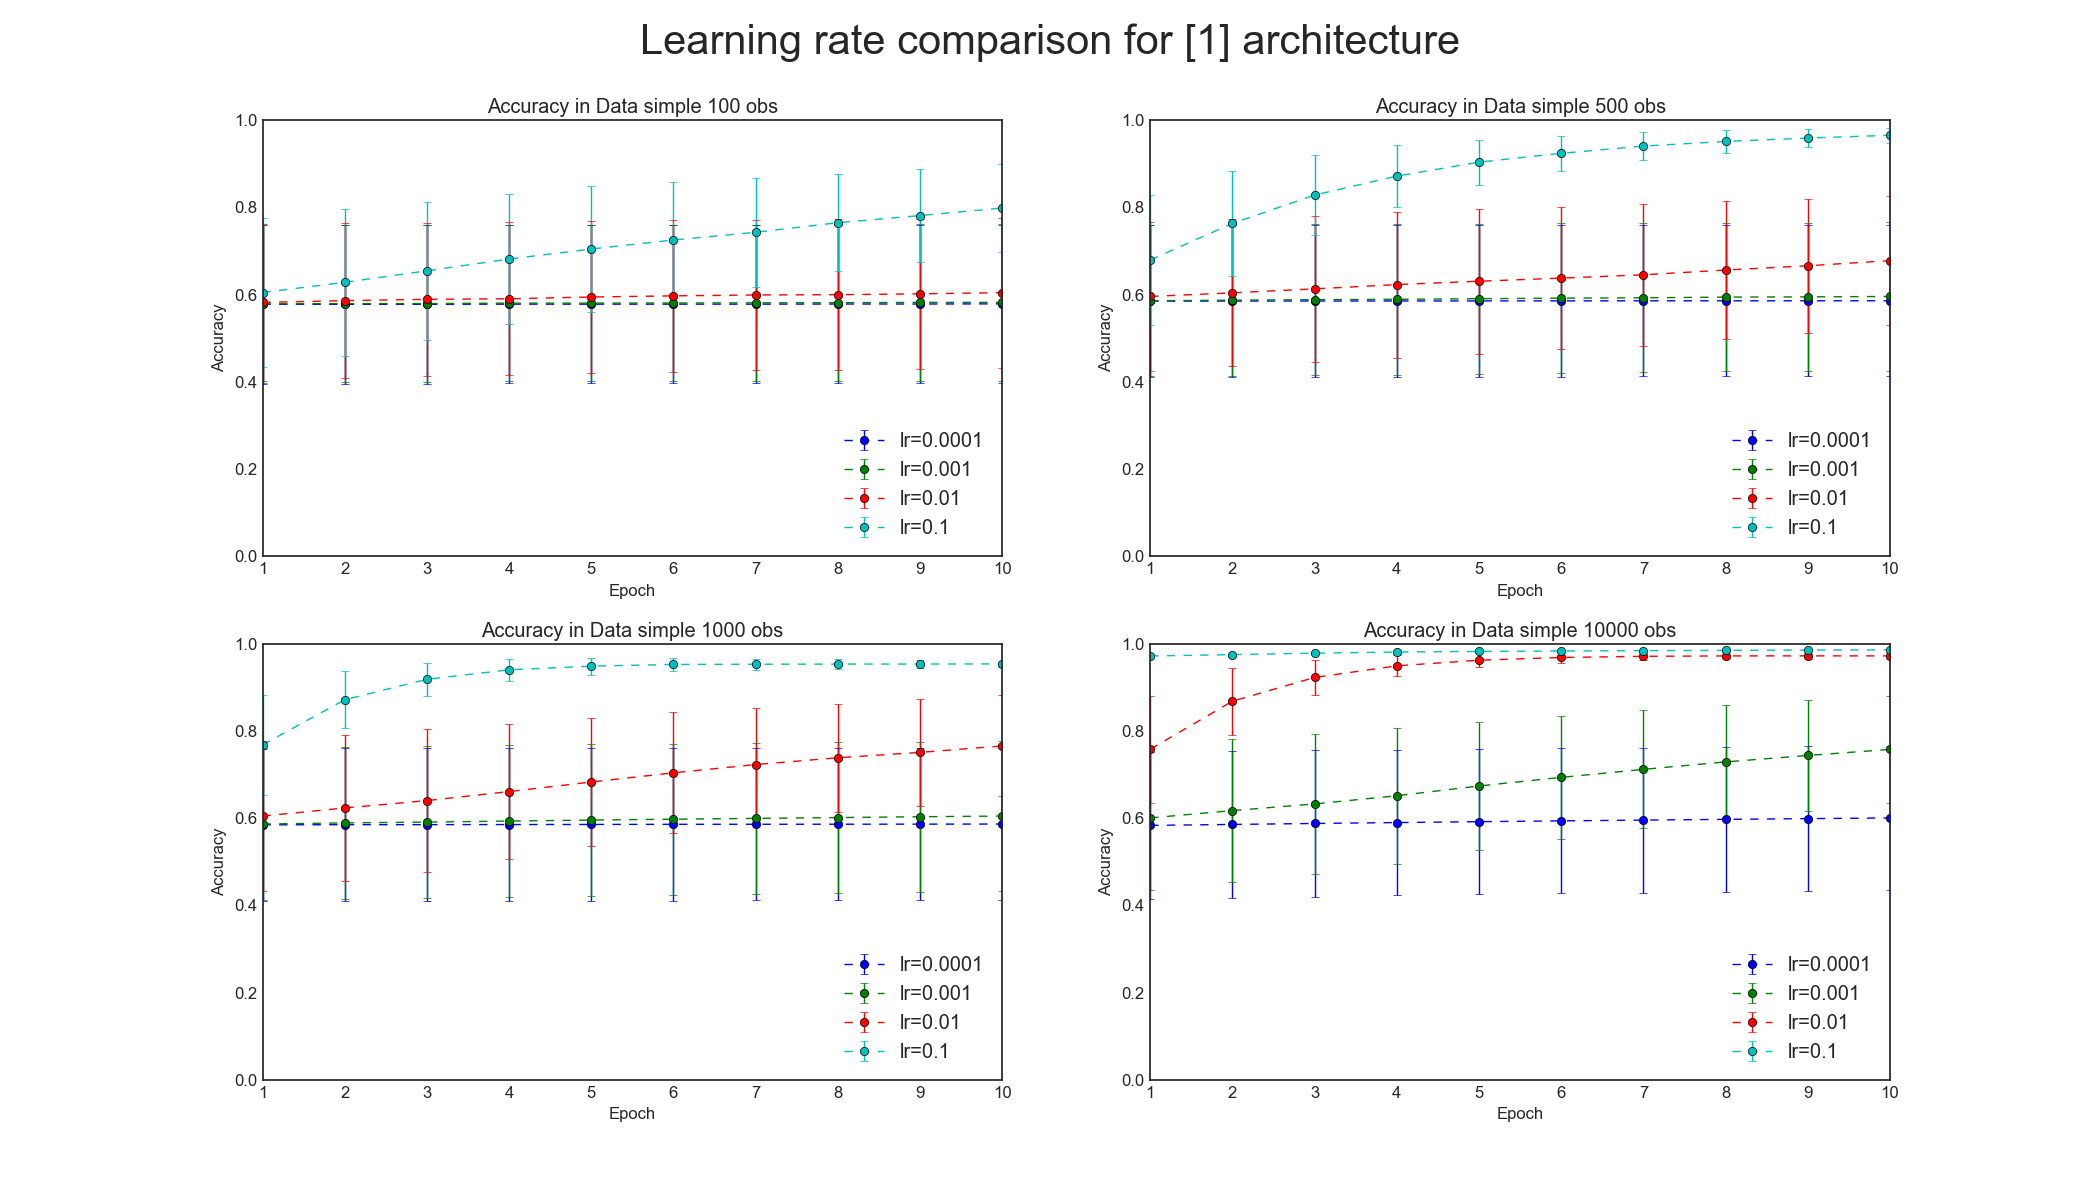
\includegraphics[width=1.4\textwidth]{results/classification/architecture-1/lr_data_simple_2020_03_24_02_34_45.png}}
   \caption{Mean accuracy achieved on the test set.}
\end{figure}

\centerline{
	\begin{tabular}{|l|llll|}
\hline
{} &     lr=0.0001 &      lr=0.001 &       lr=0.01 &        lr=0.1 \\
\hline
Data simple 100 obs   &  0.58 +- 0.18 &  0.58 +- 0.18 &  0.60 +- 0.17 &  0.80 +- 0.10 \\
Data simple 500 obs   &  0.59 +- 0.17 &  0.60 +- 0.17 &  0.68 +- 0.15 &  0.97 +- 0.02 \\
Data simple 1000 obs  &  0.59 +- 0.17 &  0.60 +- 0.17 &  0.77 +- 0.12 &  0.95 +- 0.01 \\
Data simple 10000 obs &  0.60 +- 0.17 &  0.76 +- 0.12 &  0.97 +- 0.01 &  0.99 +- 0.00 \\
\hline
\end{tabular}
}
\vspace{1em}
\begin{center}
	\textbf{Table: }The best accuracy achieved on the test set.
\end{center}


\newpage
% ----------------- AF ACTIVATION DATA  -------------------------
\begin{figure}[!ht]
    \noindent\makebox[\textwidth]{%
   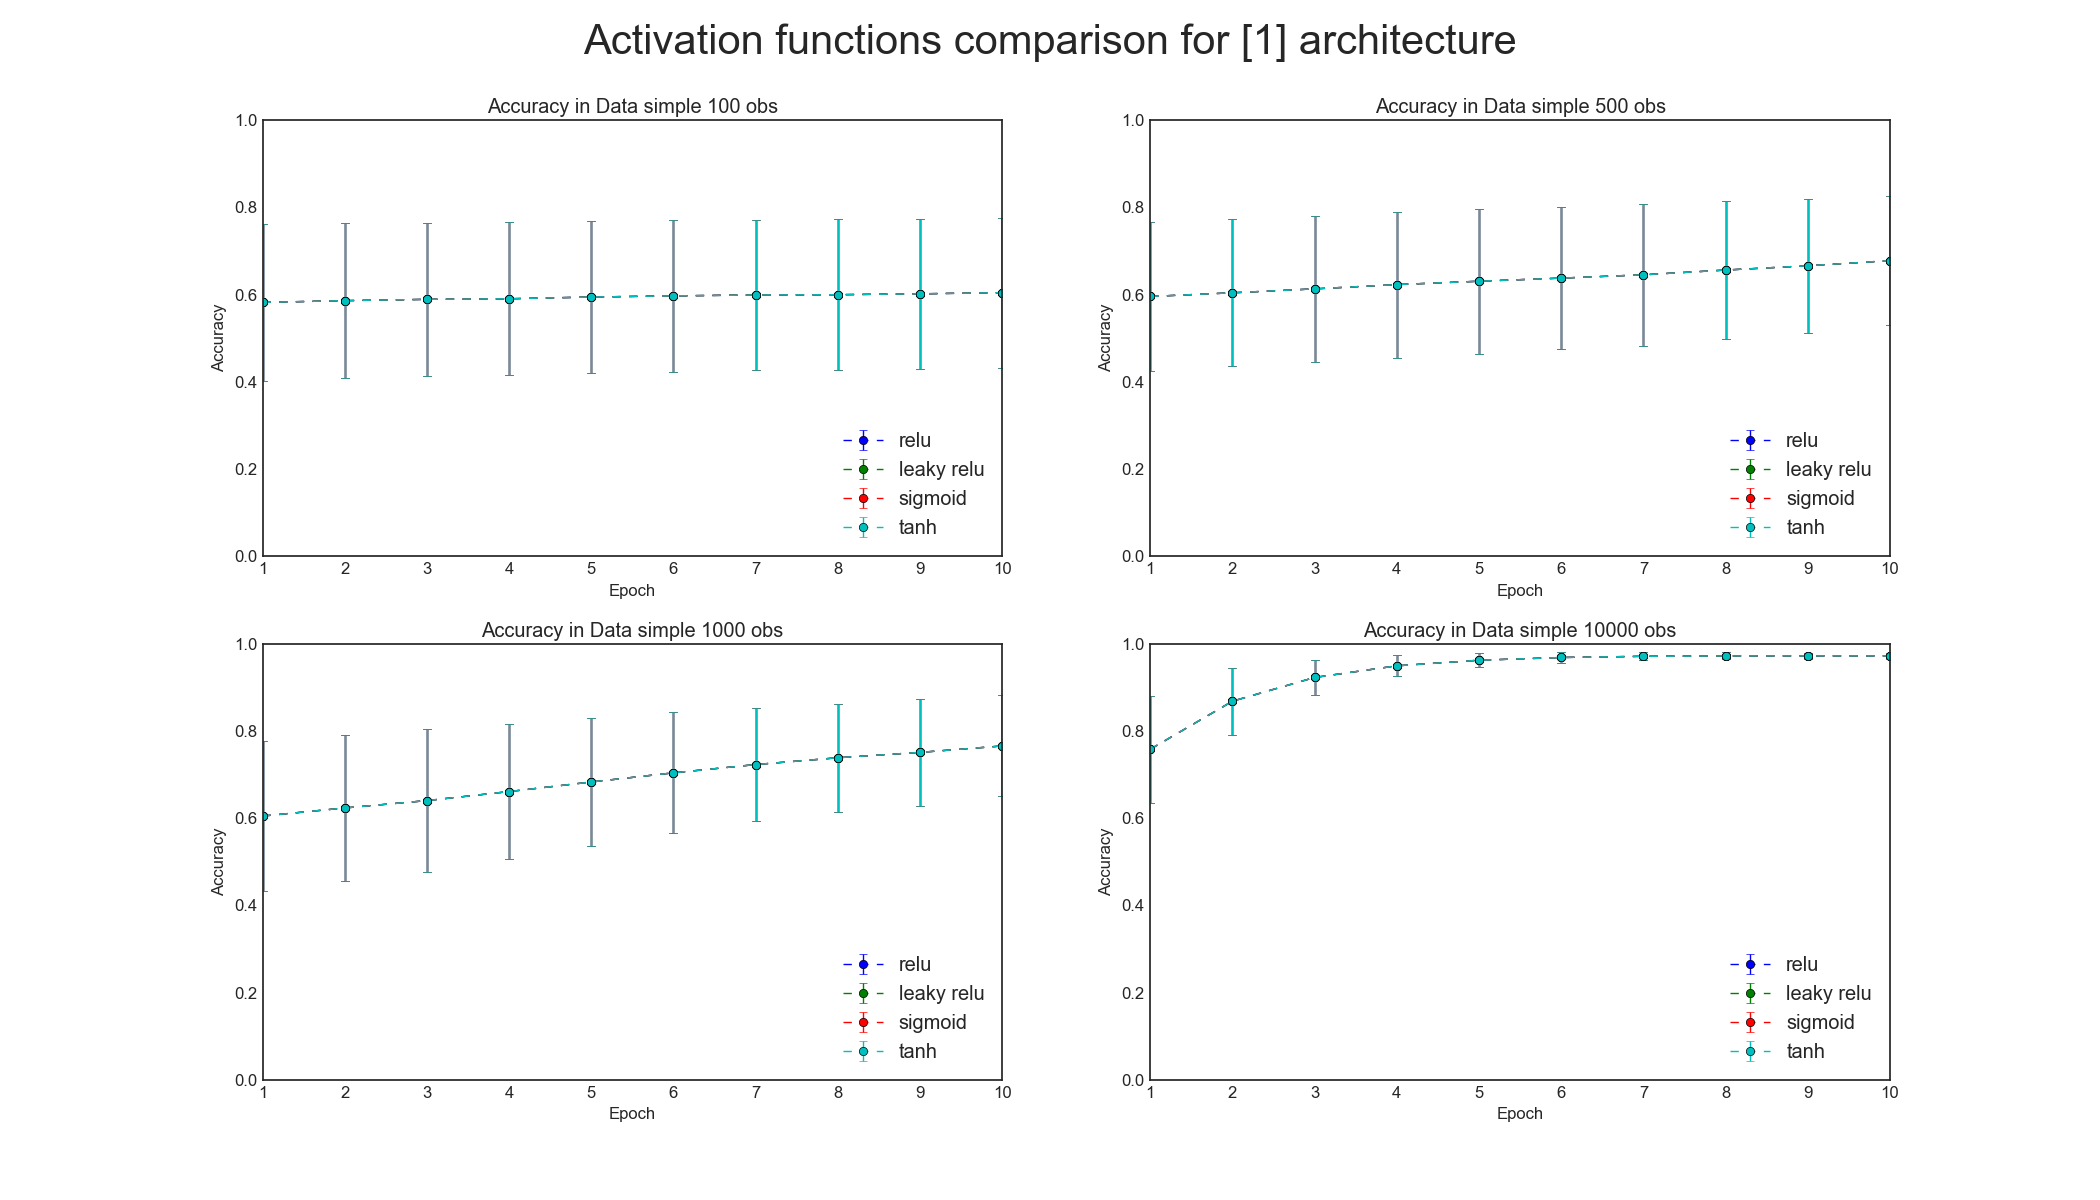
\includegraphics[width=1.4\textwidth]{results/classification/architecture-1/activation_function_data_simple_2020_03_24_02_34_46.png}}
   \caption{Mean accuracy achieved on the test set.}
\end{figure}


\centerline{
	\begin{tabular}{|l|llll|}
\hline
{} &          relu &    leaky relu &       sigmoid &          tanh \\
\hline
Data simple 100 obs   &  0.60 +- 0.17 &  0.60 +- 0.17 &  0.60 +- 0.17 &  0.60 +- 0.17 \\
Data simple 500 obs   &  0.68 +- 0.15 &  0.68 +- 0.15 &  0.68 +- 0.15 &  0.68 +- 0.15 \\
Data simple 1000 obs  &  0.77 +- 0.12 &  0.77 +- 0.12 &  0.77 +- 0.12 &  0.77 +- 0.12 \\
Data simple 10000 obs &  0.97 +- 0.01 &  0.97 +- 0.01 &  0.97 +- 0.01 &  0.97 +- 0.01 \\
\hline
\end{tabular}
}


\newpage
% ----------------- INERTIA ACTIVATION DATA  -------------------------
\begin{figure}[!ht]
    \noindent\makebox[\textwidth]{%
   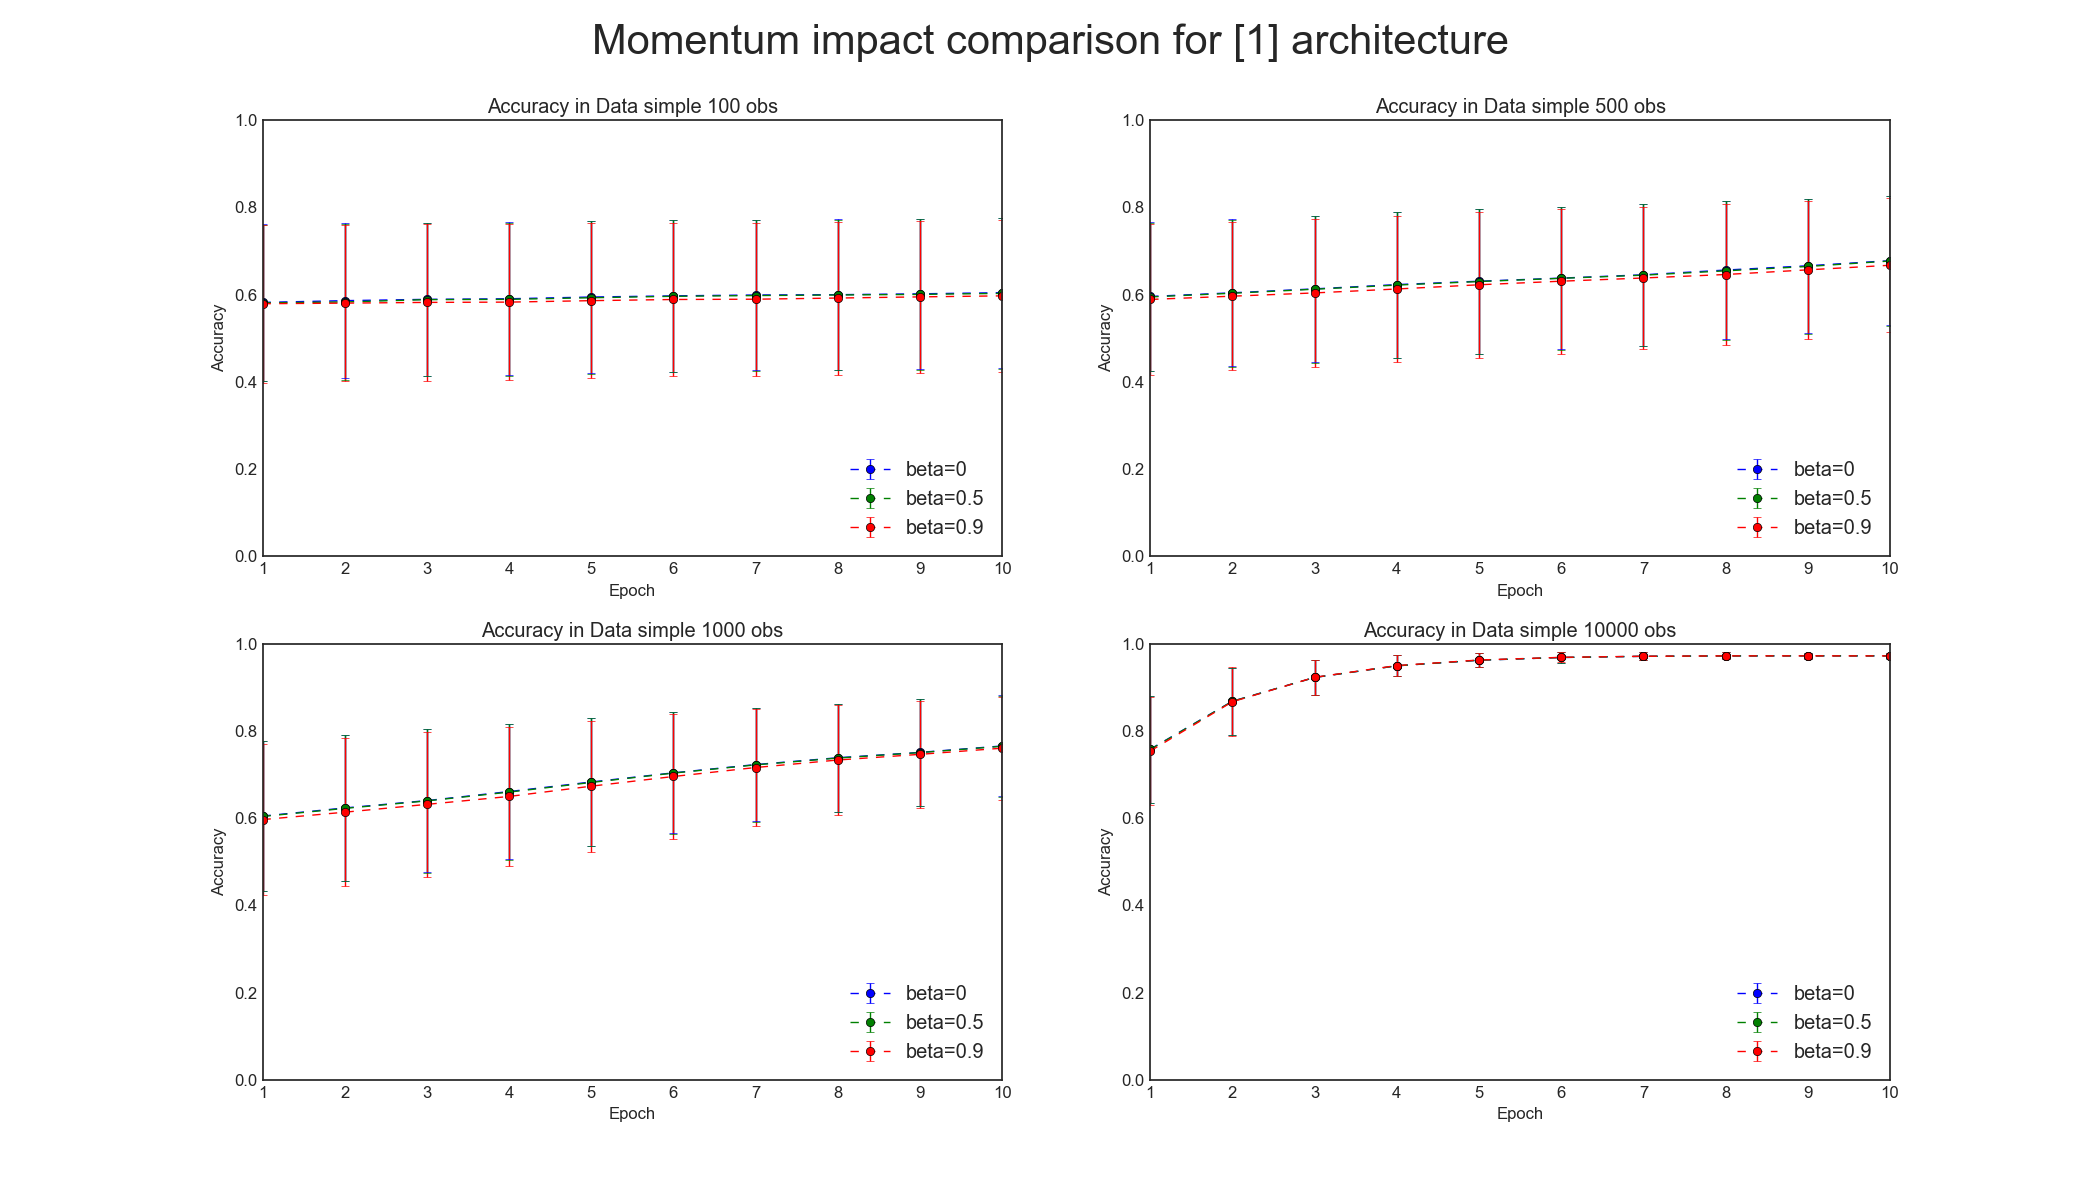
\includegraphics[width=1.4\textwidth]{results/classification/architecture-1/inertia_data_simple_2020_03_24_02_34_46.png}}
   \caption{Mean accuracy achieved on the test set.}
\end{figure}


\centerline{
\begin{tabular}{|l|lll|}
\hline
{} &        beta=0 &      beta=0.5 &      beta=0.9 \\
\hline
Data simple 100 obs   &  0.60 +- 0.17 &  0.60 +- 0.17 &  0.60 +- 0.17 \\
Data simple 500 obs   &  0.68 +- 0.15 &  0.68 +- 0.15 &  0.67 +- 0.15 \\
Data simple 1000 obs  &  0.77 +- 0.12 &  0.76 +- 0.12 &  0.76 +- 0.12 \\
Data simple 10000 obs &  0.97 +- 0.01 &  0.97 +- 0.01 &  0.97 +- 0.01 \\
\hline
\end{tabular}
}

\newpage
% ----------------- BS ACTIVATION DATA  -------------------------
\begin{figure}[!ht]
    \noindent\makebox[\textwidth]{%
   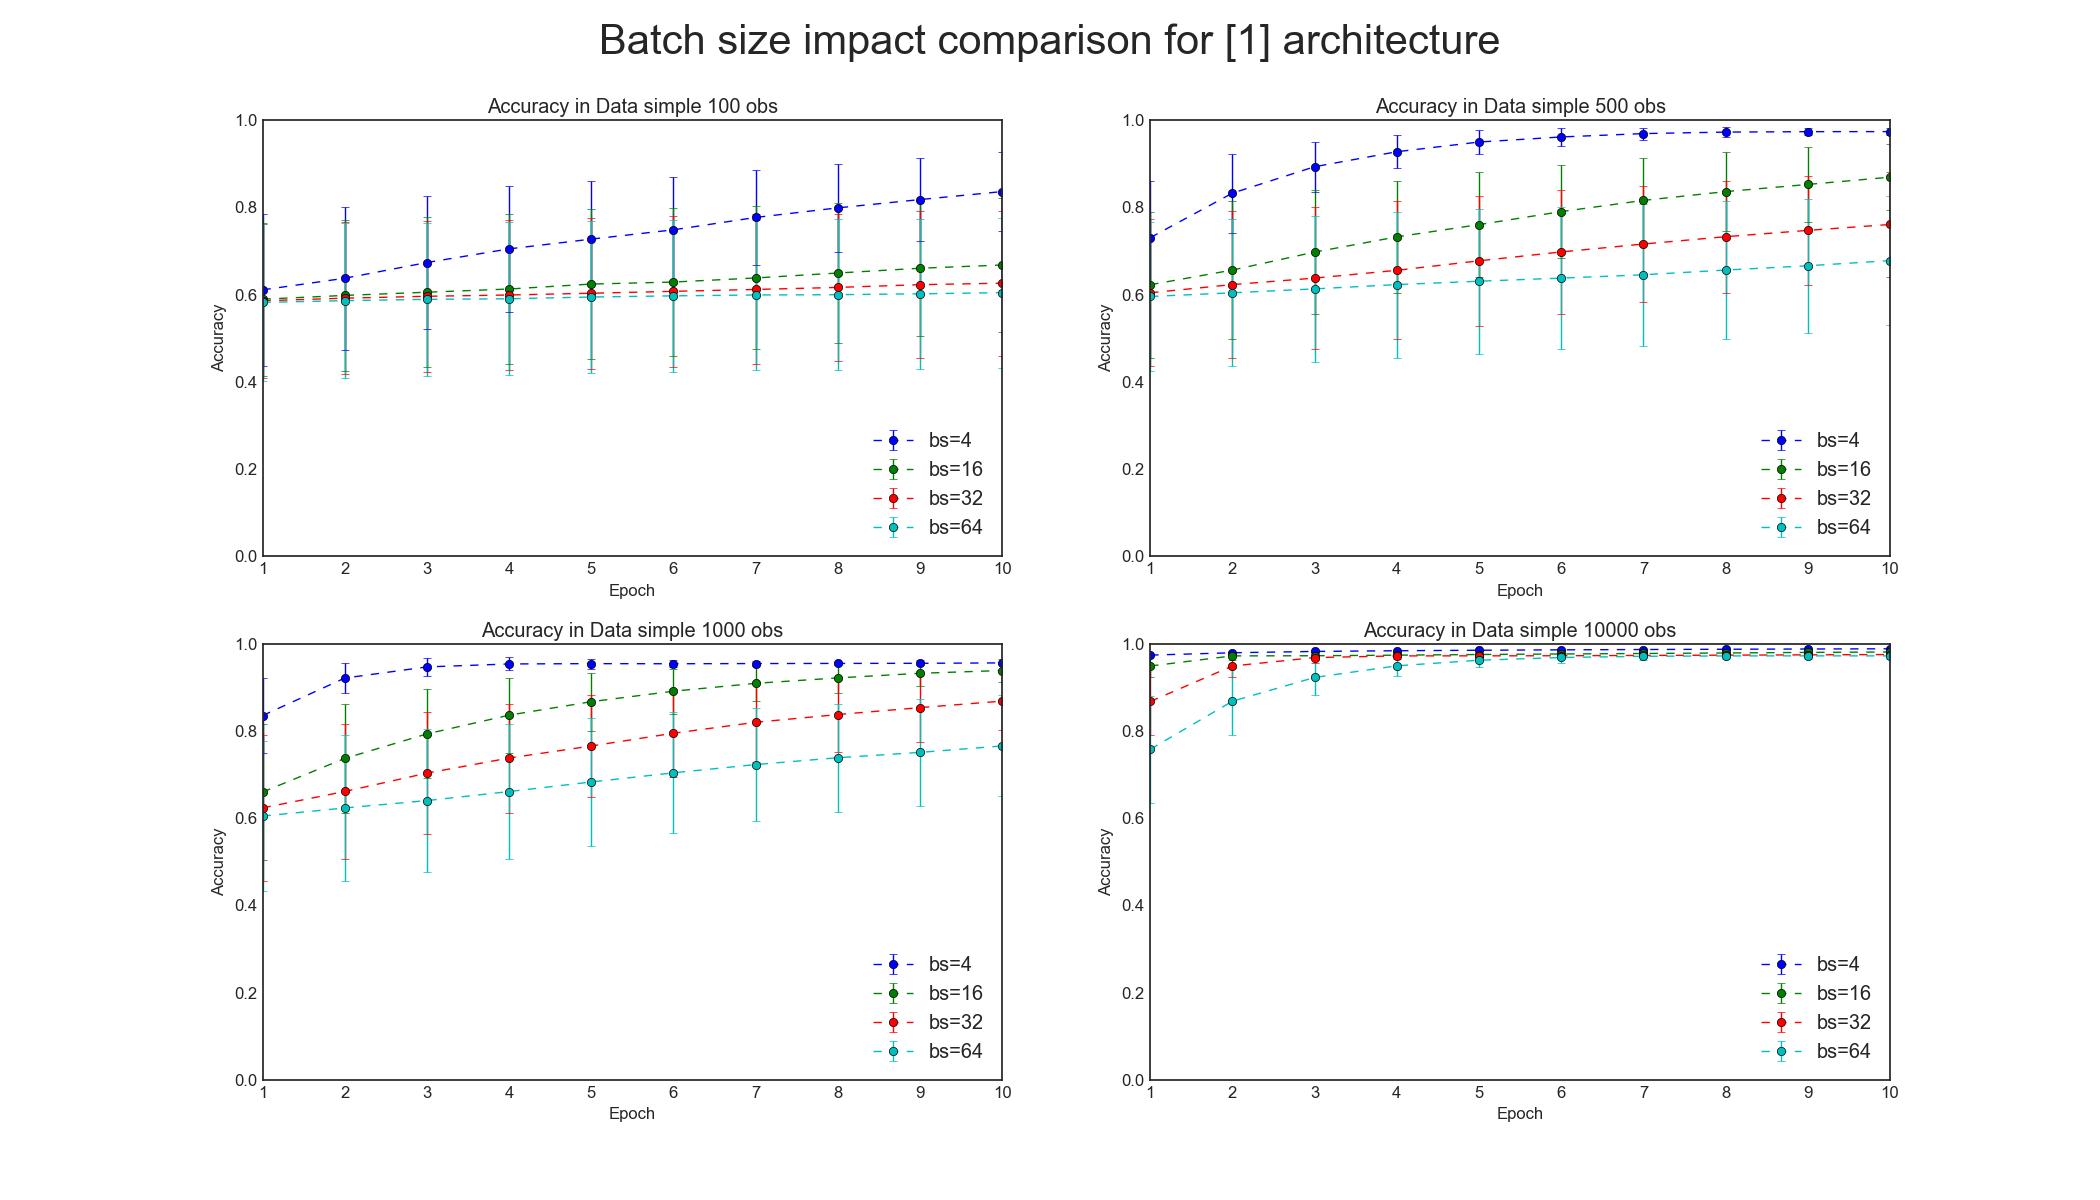
\includegraphics[width=1.4\textwidth]{results/classification/architecture-1/batch_size_data_simple_2020_03_24_02_34_46.png}}
   \caption{Mean accuracy achieved on the test set.}
\end{figure}

\centerline{
\begin{tabular}{|l|llll|}
\hline
{} &          bs=4 &         bs=16 &         bs=32 &         bs=64 \\
\hline
Data simple 100 obs   &  0.84 +- 0.09 &  0.67 +- 0.15 &  0.63 +- 0.17 &  0.60 +- 0.17 \\
Data simple 500 obs   &  0.97 +- 0.01 &  0.87 +- 0.08 &  0.76 +- 0.12 &  0.68 +- 0.15 \\
Data simple 1000 obs  &  0.96 +- 0.00 &  0.94 +- 0.03 &  0.87 +- 0.07 &  0.77 +- 0.12 \\
Data simple 10000 obs &  0.99 +- 0.00 &  0.98 +- 0.00 &  0.98 +- 0.00 &  0.97 +- 0.01 \\
\hline
\end{tabular}
}



\newpage
\subsubsection{Architecture 2}
\[[5]\]
One hidden layer with 5 neurons.

% ----------------- LR ACTIVATION DATA  -------------------------

\begin{figure}[!ht]
    \noindent\makebox[\textwidth]{%
   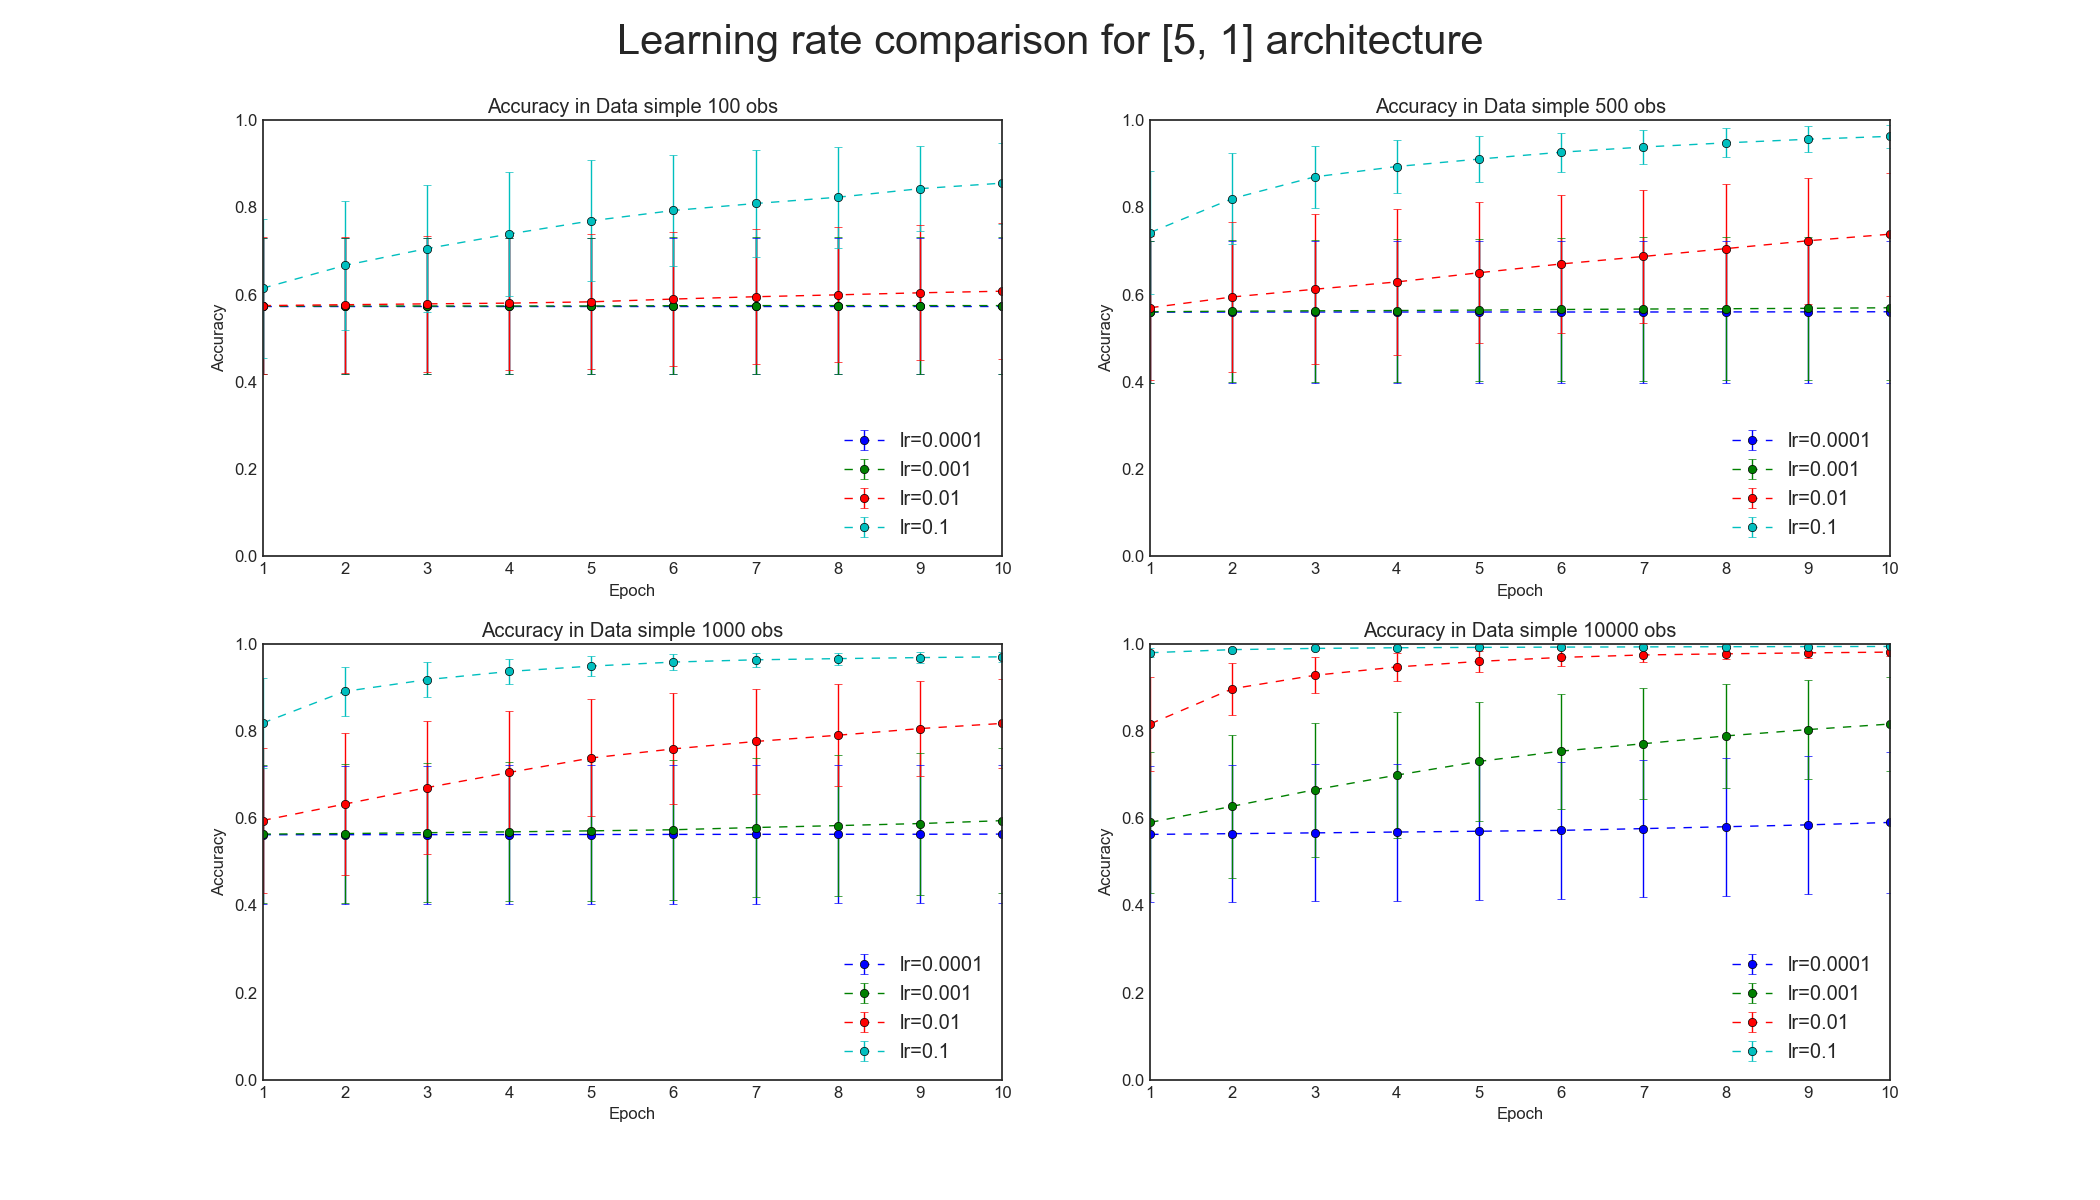
\includegraphics[width=1.4\textwidth]{results/classification/architecture-2/lr_data_simple_2020_03_24_02_41_43.png}}
   \caption{Mean accuracy achieved on the test set.}
\end{figure}

\centerline{\begin{tabular}{lllll}
\hline
{} &     lr=0.0001 &      lr=0.001 &       lr=0.01 &        lr=0.1 \\
\hline
Data simple 100 obs   &  0.57 +- 0.16 &  0.57 +- 0.16 &  0.61 +- 0.16 &  0.86 +- 0.09 \\
Data simple 500 obs   &  0.56 +- 0.16 &  0.57 +- 0.17 &  0.74 +- 0.14 &  0.96 +- 0.03 \\
Data simple 1000 obs  &  0.56 +- 0.16 &  0.59 +- 0.17 &  0.82 +- 0.10 &  0.97 +- 0.01 \\
Data simple 10000 obs &  0.59 +- 0.16 &  0.82 +- 0.11 &  0.98 +- 0.01 &  0.99 +- 0.00 \\
\hline
\end{tabular}}

\newpage
% ----------------- AF ACTIVATION DATA  -------------------------
\begin{figure}[!ht]
    \noindent\makebox[\textwidth]{%
   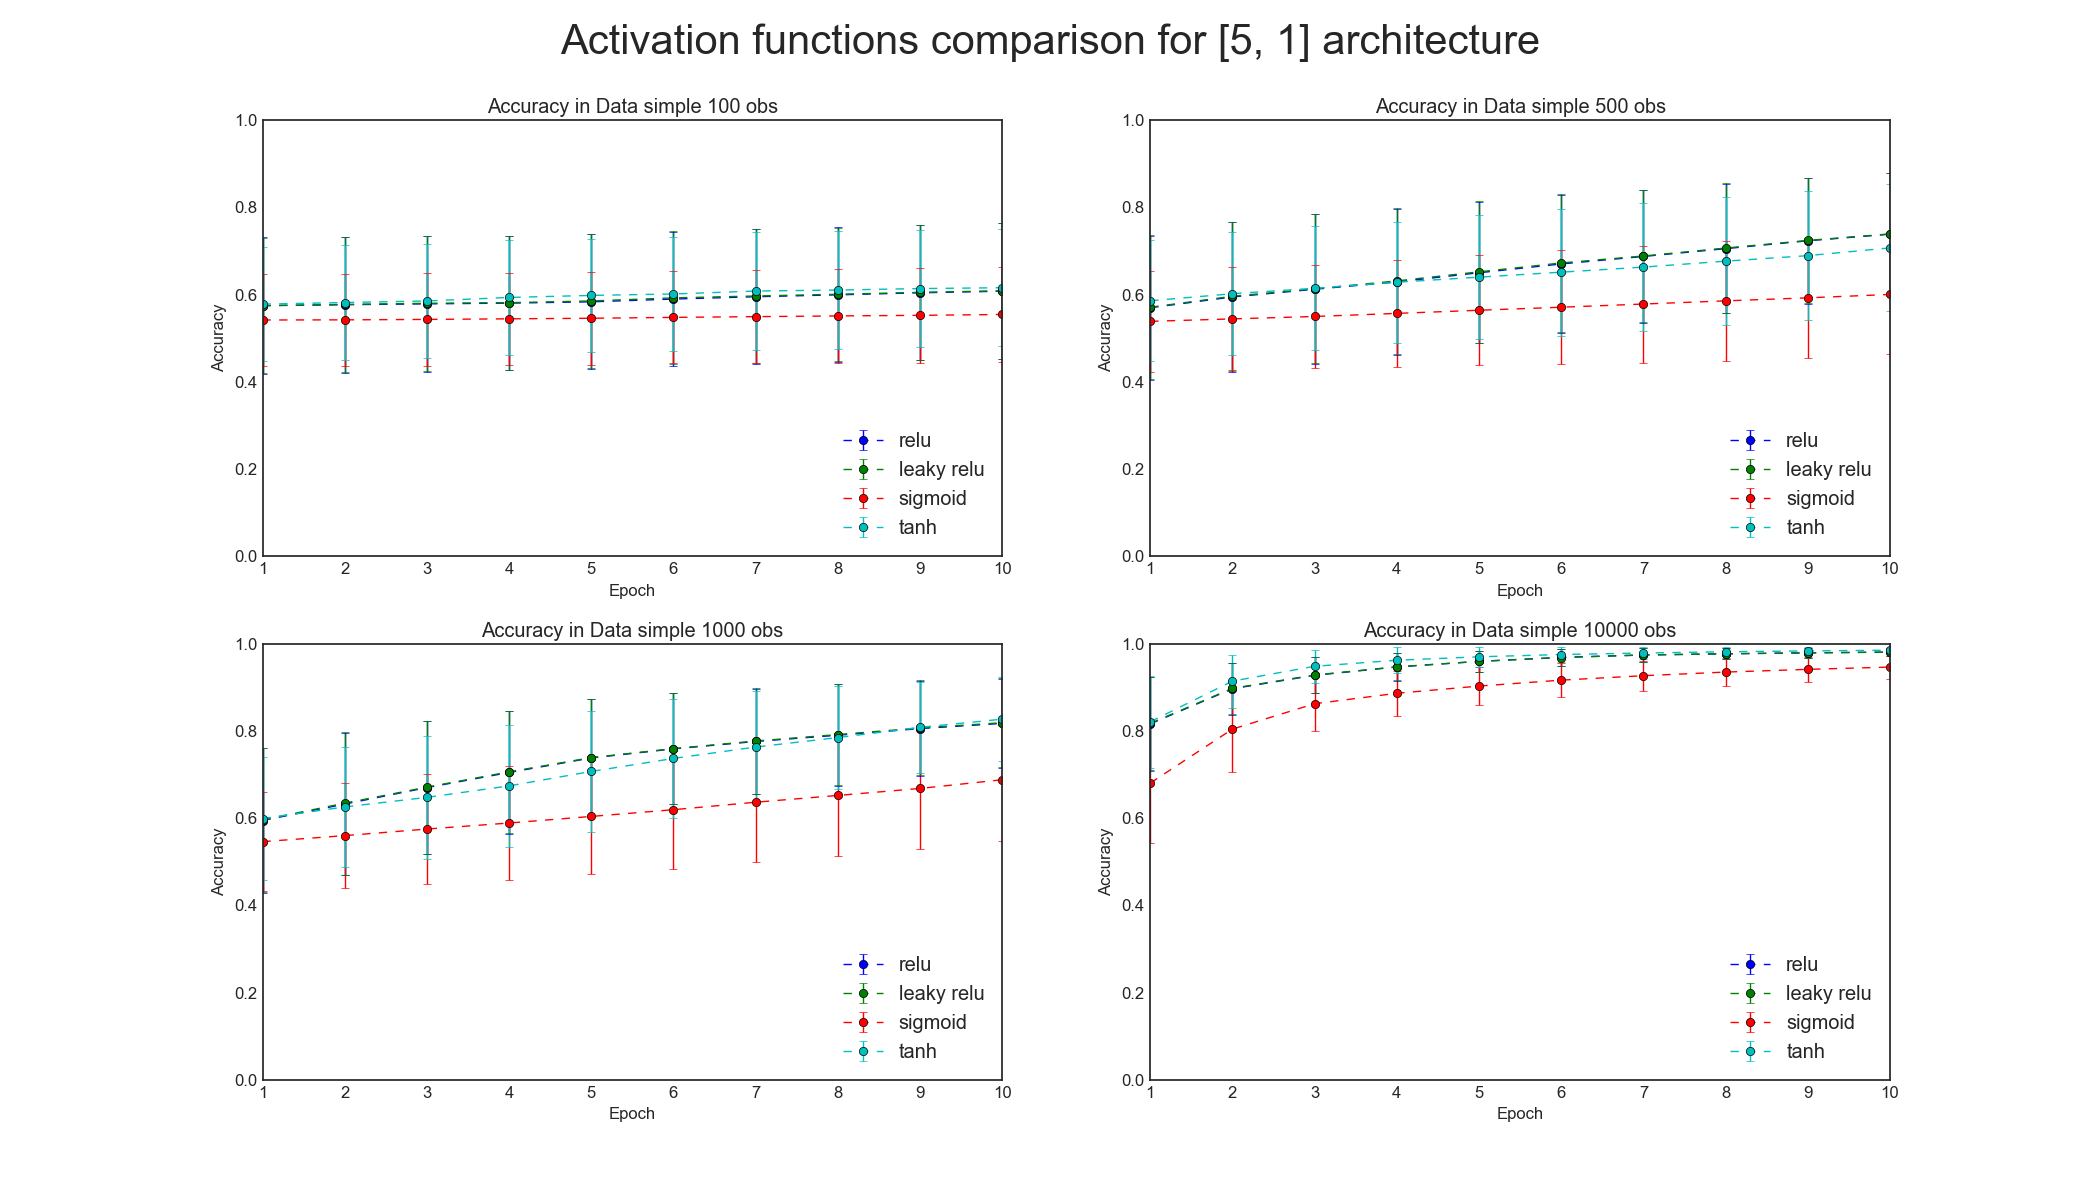
\includegraphics[width=1.4\textwidth]{results/classification/architecture-2/activation_function_data_simple_2020_03_24_02_41_44.png}}
   \caption{Mean accuracy achieved on the test set.}
\end{figure}


\centerline{
\begin{tabular}{lllll}
\hline
{} &          relu &    leaky relu &       sigmoid &          tanh \\
\hline
Data simple 100 obs   &  0.61 +- 0.16 &  0.61 +- 0.16 &  0.55 +- 0.11 &  0.62 +- 0.13 \\
Data simple 500 obs   &  0.74 +- 0.14 &  0.74 +- 0.14 &  0.60 +- 0.14 &  0.71 +- 0.15 \\
Data simple 1000 obs  &  0.82 +- 0.10 &  0.82 +- 0.10 &  0.69 +- 0.14 &  0.83 +- 0.10 \\
Data simple 10000 obs &  0.98 +- 0.01 &  0.98 +- 0.01 &  0.95 +- 0.03 &  0.98 +- 0.01 \\
\hline
\end{tabular}
}

\newpage
% ----------------- INERTIA ACTIVATION DATA  -------------------------
\begin{figure}[!ht]
    \noindent\makebox[\textwidth]{%
   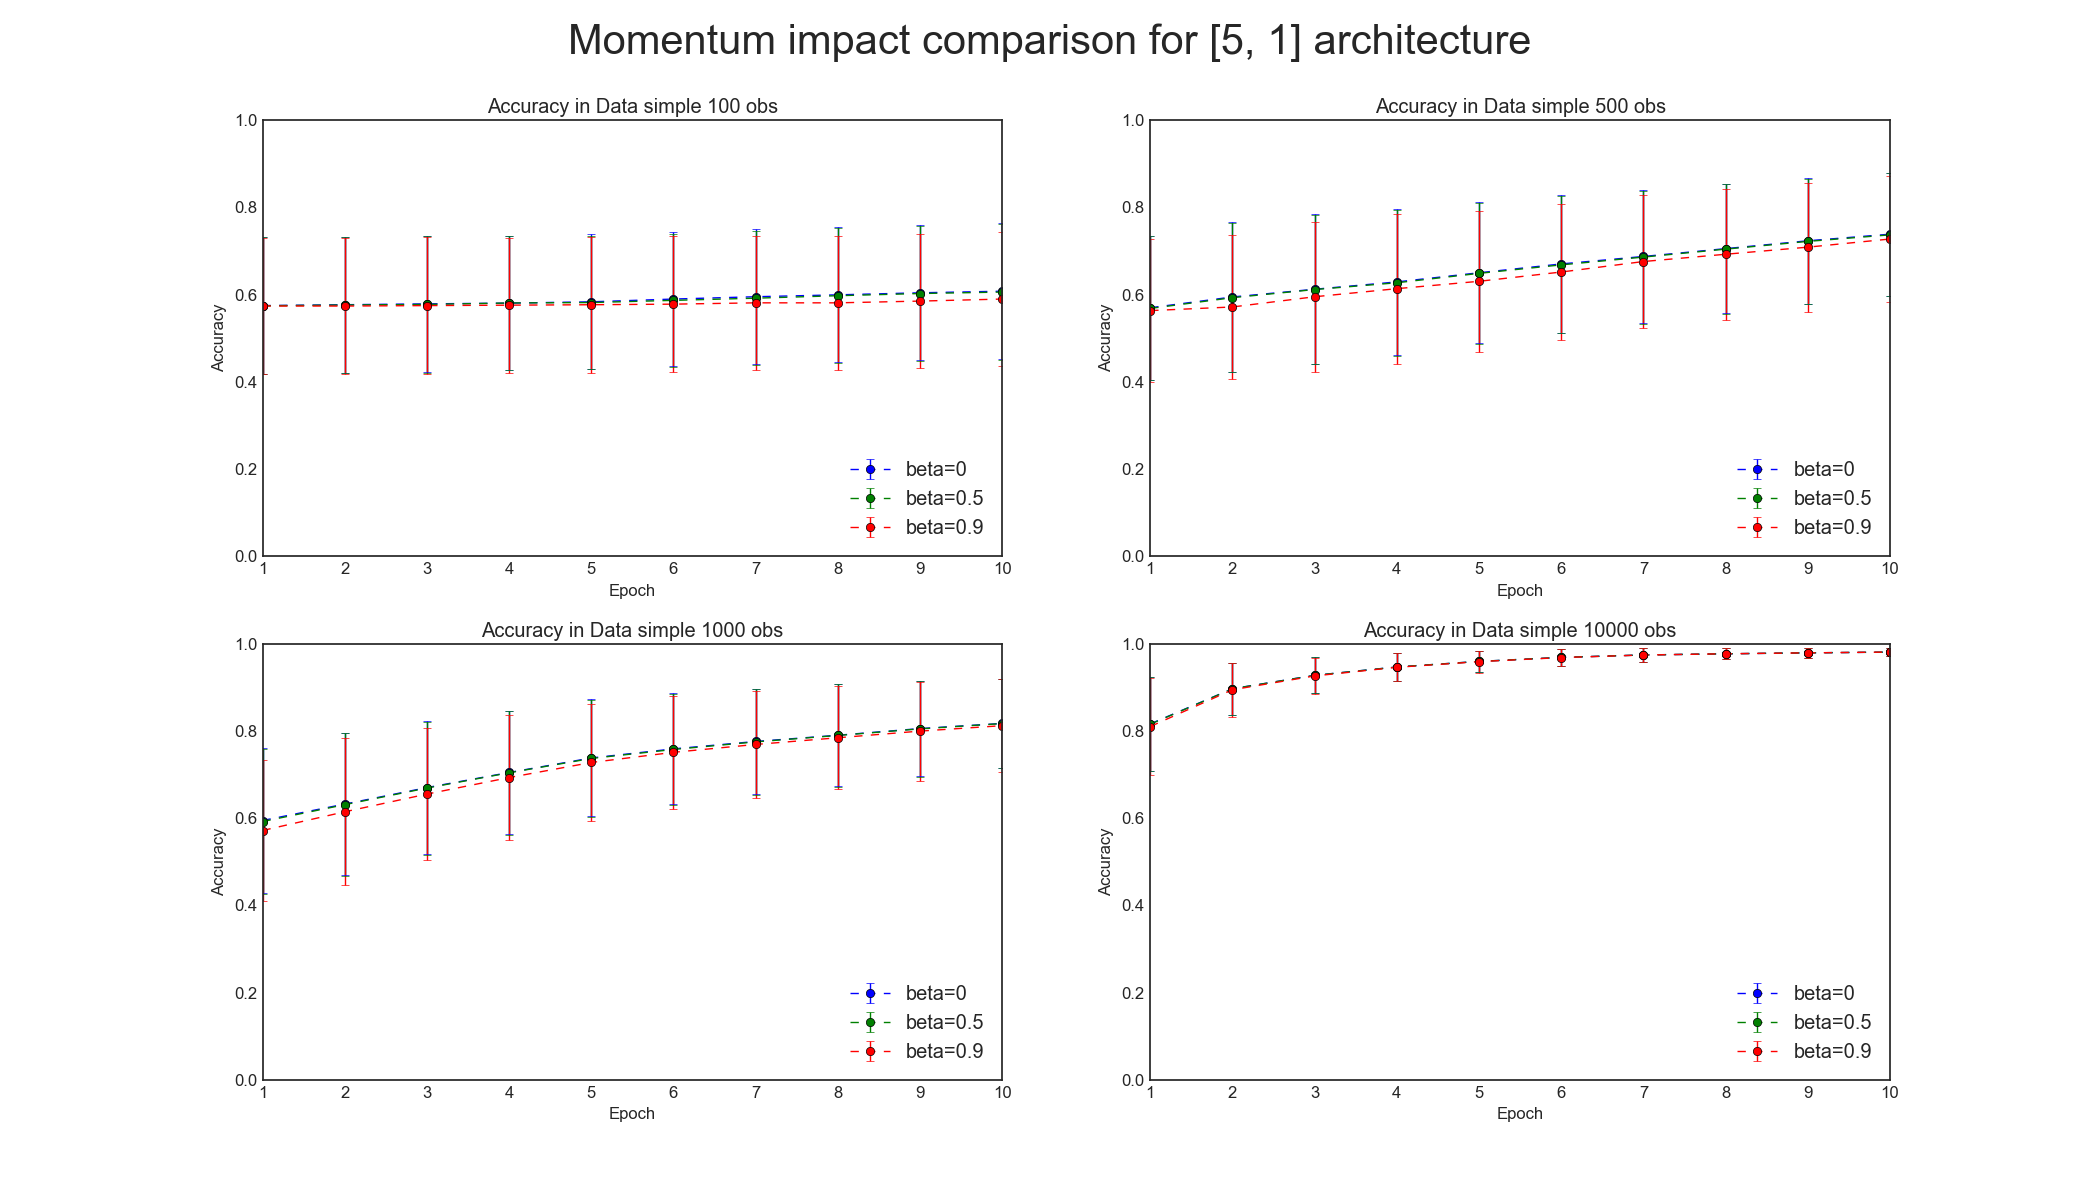
\includegraphics[width=1.4\textwidth]{results/classification/architecture-2/inertia_data_simple_2020_03_24_02_41_44.png}}
   \caption{Mean accuracy achieved on the test set.}
\end{figure}


\centerline{
\begin{tabular}{llll}
\hline
{} &        beta=0 &      beta=0.5 &      beta=0.9 \\
\hline
Data simple 100 obs   &  0.61 +- 0.16 &  0.61 +- 0.16 &  0.59 +- 0.15 \\
Data simple 500 obs   &  0.74 +- 0.14 &  0.74 +- 0.14 &  0.73 +- 0.14 \\
Data simple 1000 obs  &  0.82 +- 0.10 &  0.82 +- 0.10 &  0.81 +- 0.11 \\
Data simple 10000 obs &  0.98 +- 0.01 &  0.98 +- 0.01 &  0.98 +- 0.01 \\
\hline
\end{tabular}
}

\newpage
% ----------------- BS ACTIVATION DATA  -------------------------
\begin{figure}[!ht]
    \noindent\makebox[\textwidth]{%
   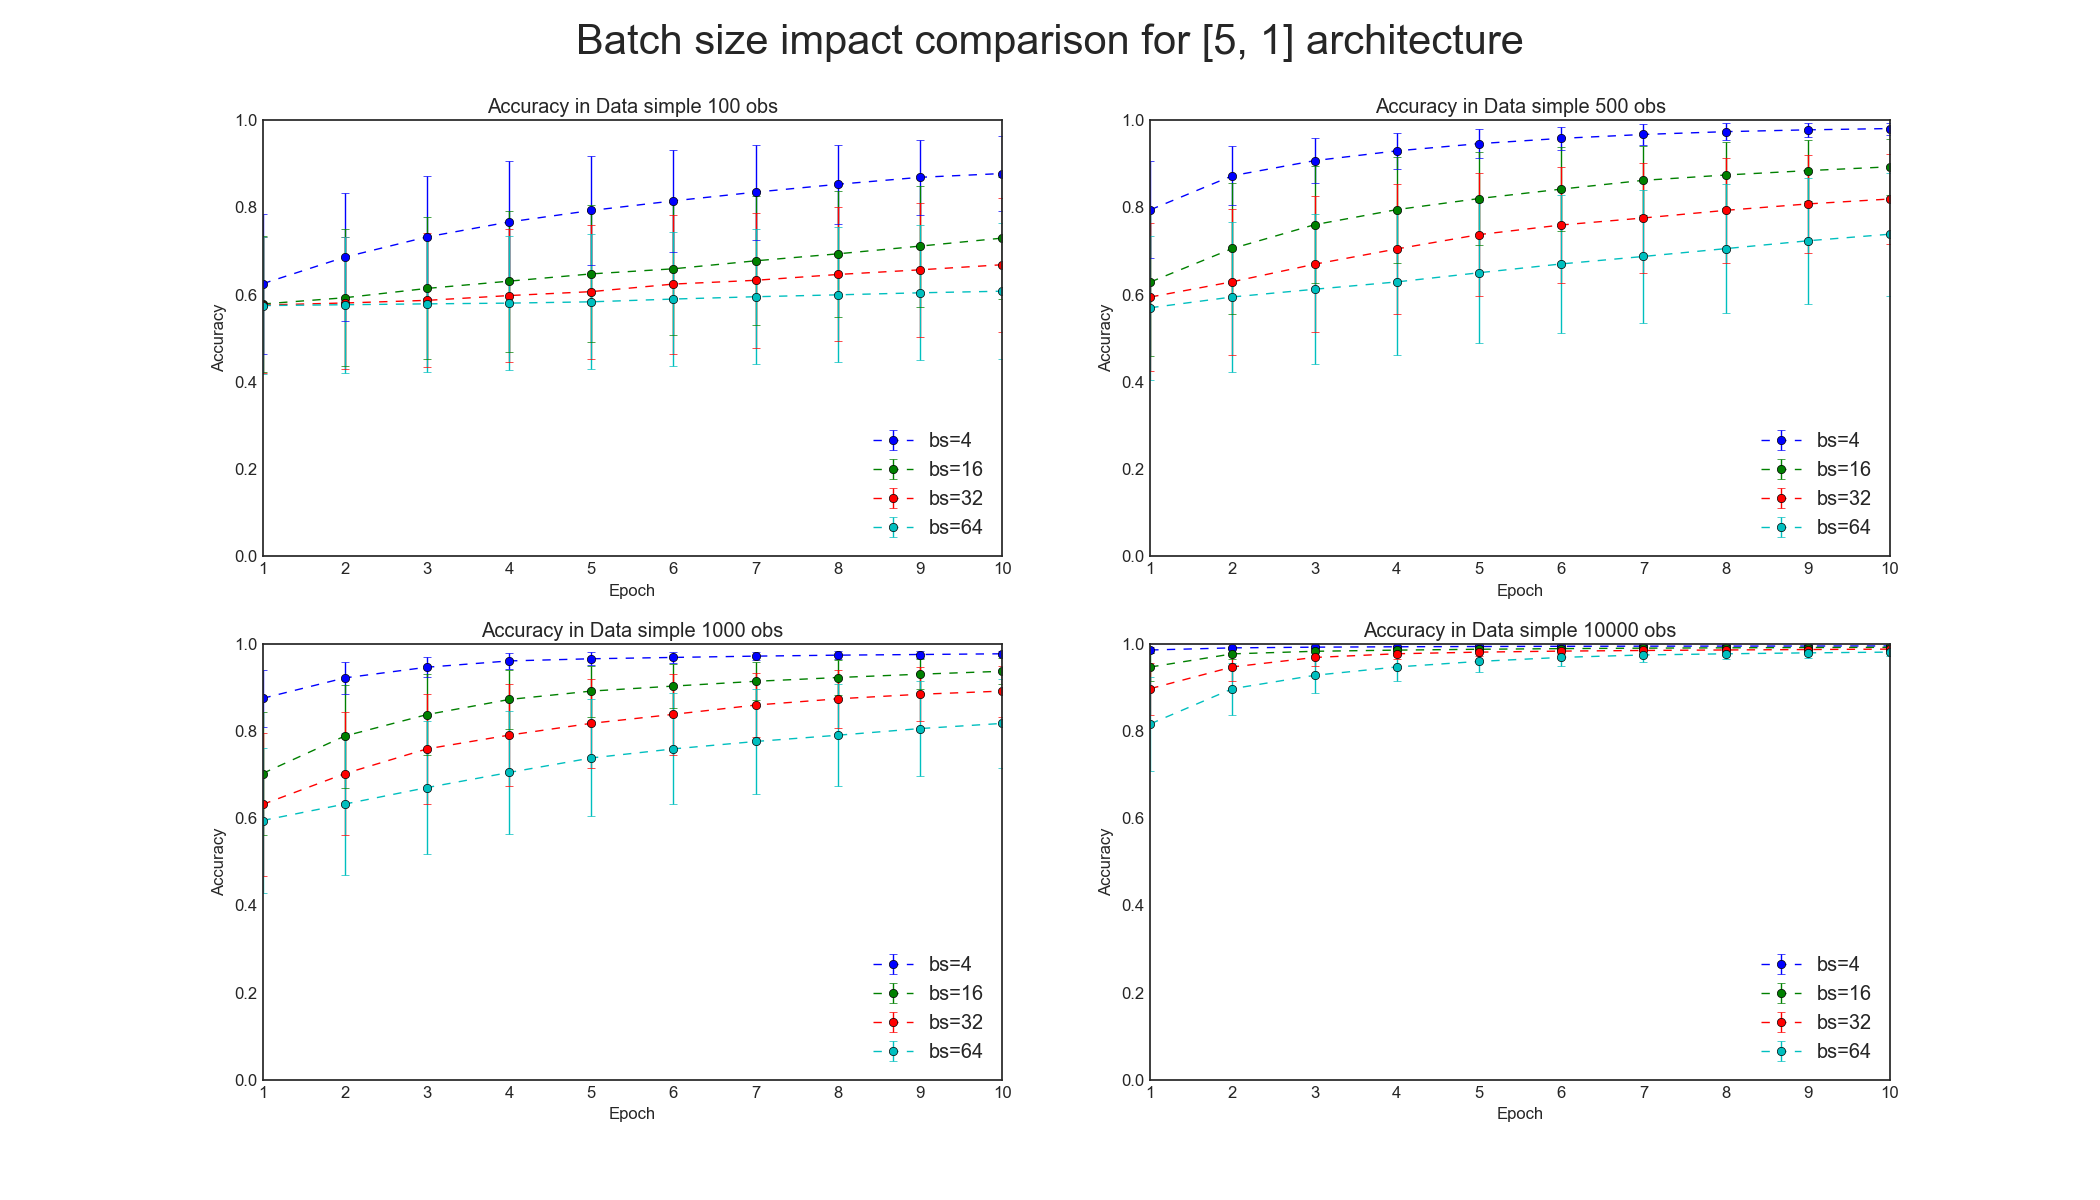
\includegraphics[width=1.4\textwidth]{results/classification/architecture-2/batch_size_data_simple_2020_03_24_02_41_45.png}}
   \caption{Mean accuracy achieved on the test set.}
\end{figure}

\centerline{
\begin{tabular}{lllll}
\hline
{} &          bs=4 &         bs=16 &         bs=32 &         bs=64 \\
\hline
Data simple 100 obs   &  0.88 +- 0.09 &  0.73 +- 0.14 &  0.67 +- 0.15 &  0.61 +- 0.16 \\
Data simple 500 obs   &  0.98 +- 0.01 &  0.89 +- 0.06 &  0.82 +- 0.10 &  0.74 +- 0.14 \\
Data simple 1000 obs  &  0.98 +- 0.01 &  0.94 +- 0.03 &  0.89 +- 0.06 &  0.82 +- 0.10 \\
Data simple 10000 obs &  0.99 +- 0.00 &  0.99 +- 0.00 &  0.99 +- 0.00 &  0.98 +- 0.01 \\
\hline
\end{tabular}
}

\newpage
\subsubsection{Architecture 3}
\[[5, 5]\]
Two hidden layers, 5 neurons in each of them.

% ----------------- LR ACTIVATION DATA  -------------------------

\begin{figure}[!ht]
    \noindent\makebox[\textwidth]{%
   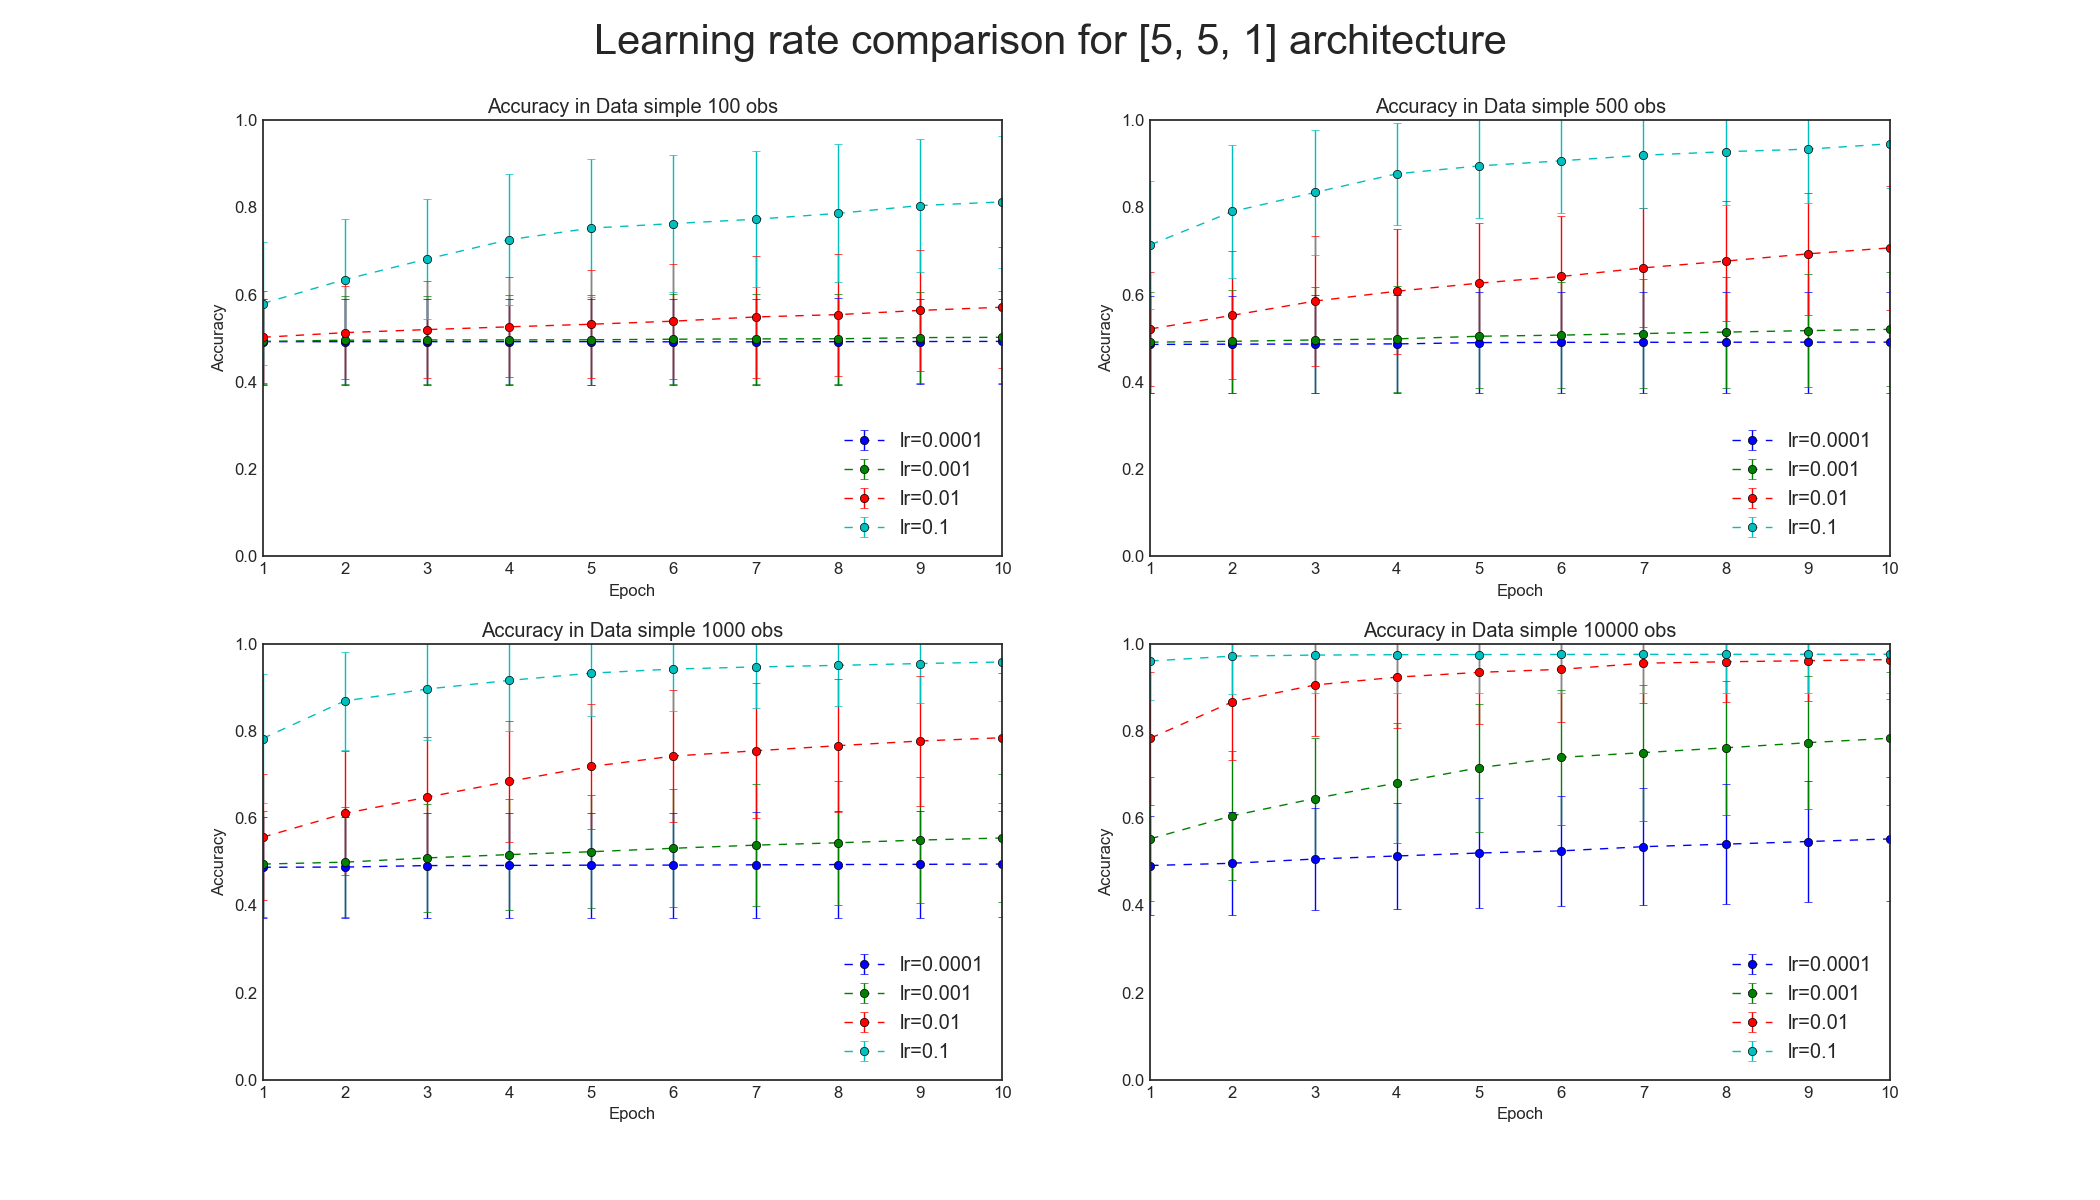
\includegraphics[width=1.4\textwidth]{results/classification/architecture-3/lr_data_simple_2020_03_24_02_49_46.png}}
   \caption{Mean accuracy achieved on the test set.}
\end{figure}

\centerline{
\begin{tabular}{lllll}
\hline
{} &     lr=0.0001 &      lr=0.001 &       lr=0.01 &        lr=0.1 \\
\hline
Data simple 100 obs   &  0.49 +- 0.10 &  0.50 +- 0.11 &  0.57 +- 0.14 &  0.81 +- 0.15 \\
Data simple 500 obs   &  0.49 +- 0.12 &  0.52 +- 0.13 &  0.71 +- 0.14 &  0.95 +- 0.10 \\
Data simple 1000 obs  &  0.49 +- 0.12 &  0.55 +- 0.15 &  0.78 +- 0.15 &  0.96 +- 0.09 \\
Data simple 10000 obs &  0.55 +- 0.14 &  0.78 +- 0.15 &  0.96 +- 0.09 &  0.98 +- 0.09 \\
\hline
\end{tabular}
}

\newpage
% ----------------- AF ACTIVATION DATA  -------------------------
\begin{figure}[!ht]
    \noindent\makebox[\textwidth]{%
   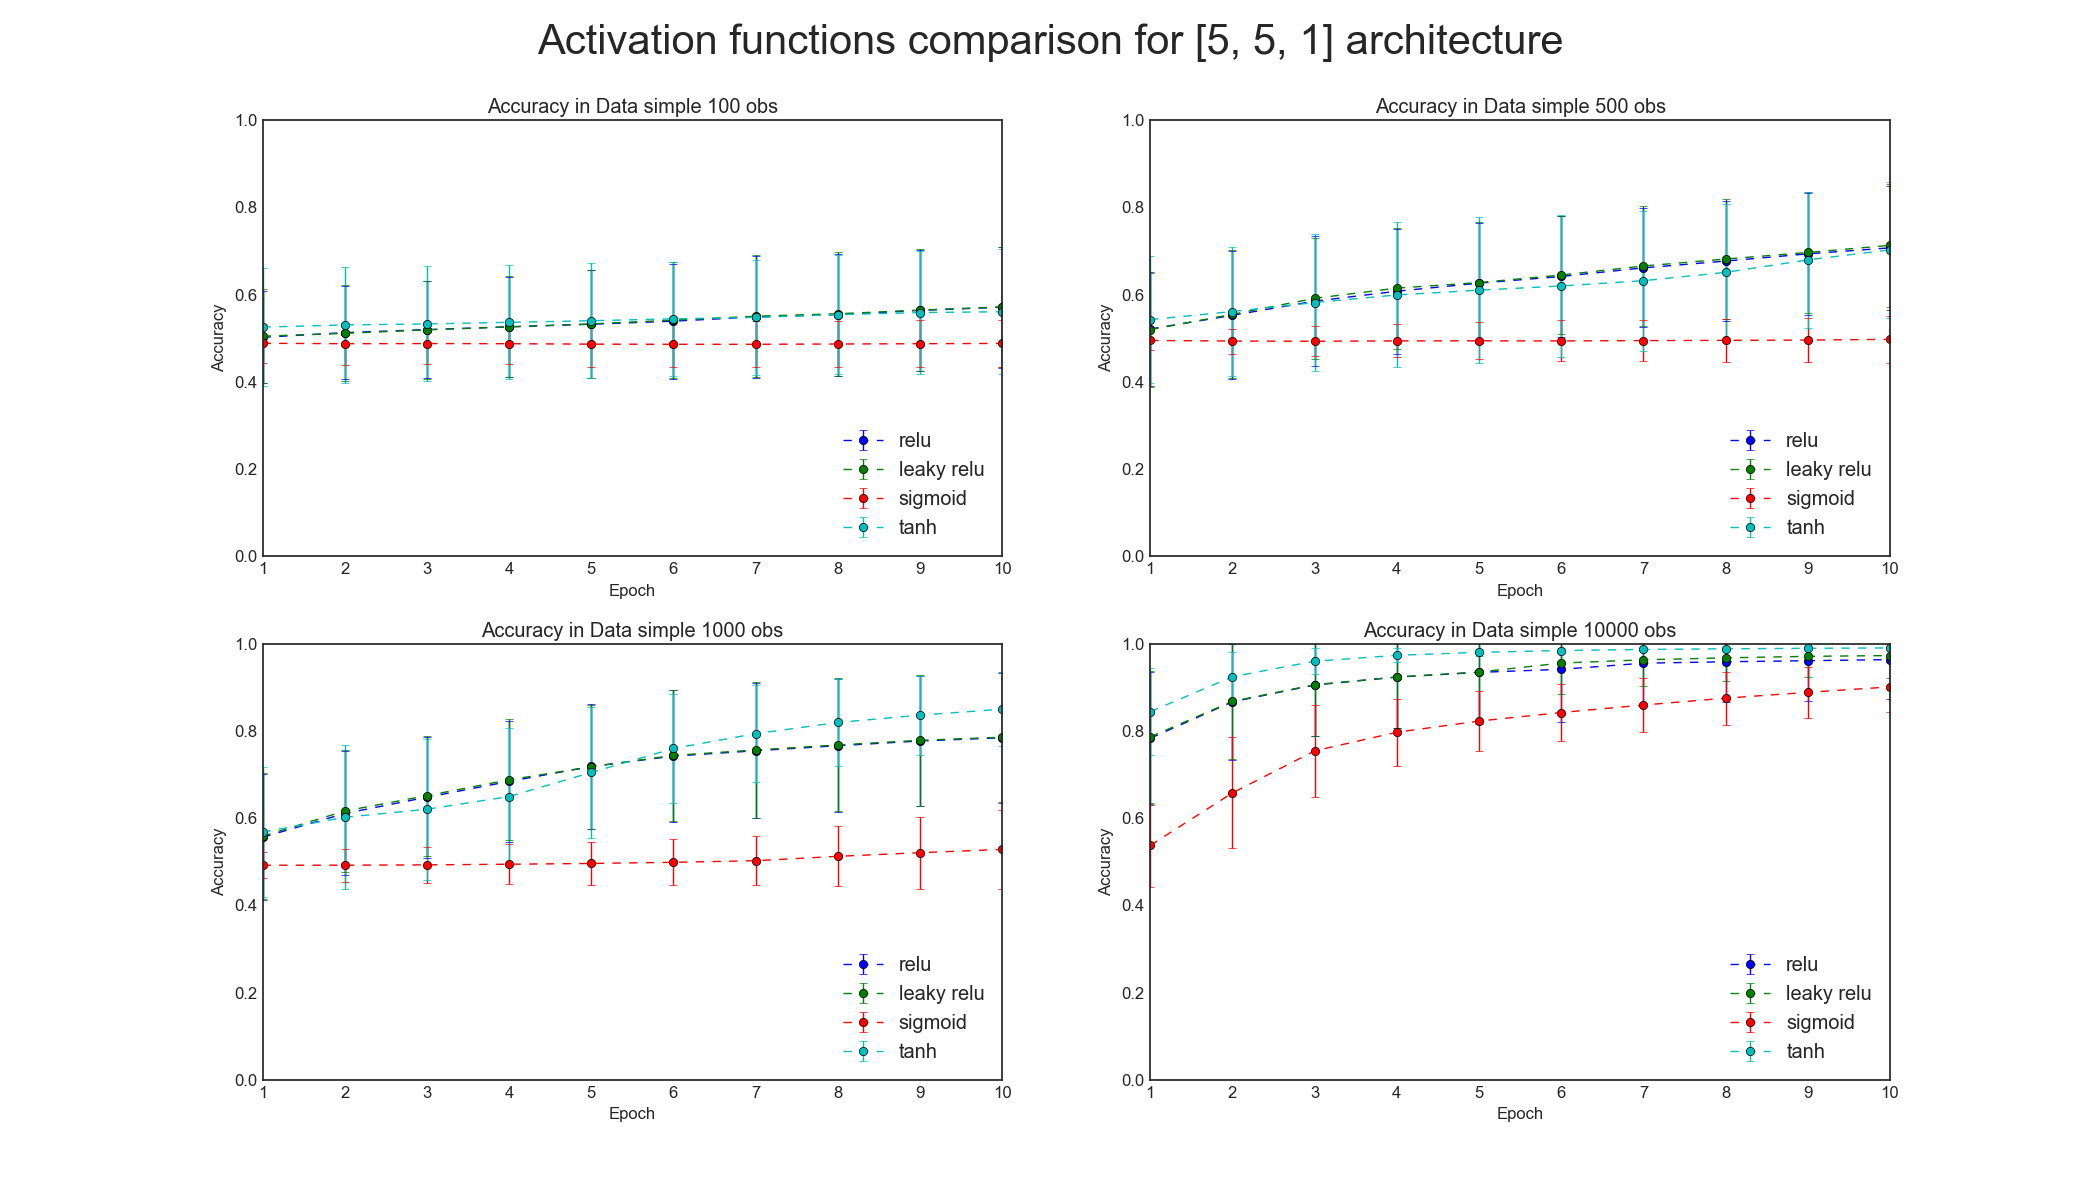
\includegraphics[width=1.4\textwidth]{results/classification/architecture-3/activation_function_data_simple_2020_03_24_02_49_47.png}}
   \caption{Mean accuracy achieved on the test set.}
\end{figure}


\centerline{
\begin{tabular}{lllll}
\hline
{} &          relu &    leaky relu &       sigmoid &          tanh \\
\hline
Data simple 100 obs   &  0.57 +- 0.14 &  0.57 +- 0.14 &  0.49 +- 0.04 &  0.56 +- 0.14 \\
Data simple 500 obs   &  0.71 +- 0.14 &  0.71 +- 0.14 &  0.50 +- 0.05 &  0.70 +- 0.16 \\
Data simple 1000 obs  &  0.78 +- 0.15 &  0.79 +- 0.15 &  0.53 +- 0.09 &  0.85 +- 0.09 \\
Data simple 10000 obs &  0.96 +- 0.09 &  0.97 +- 0.05 &  0.90 +- 0.06 &  0.99 +- 0.00 \\
\hline
\end{tabular}
}

\newpage
% ----------------- INERTIA ACTIVATION DATA  -------------------------
\begin{figure}[!ht]
    \noindent\makebox[\textwidth]{%
   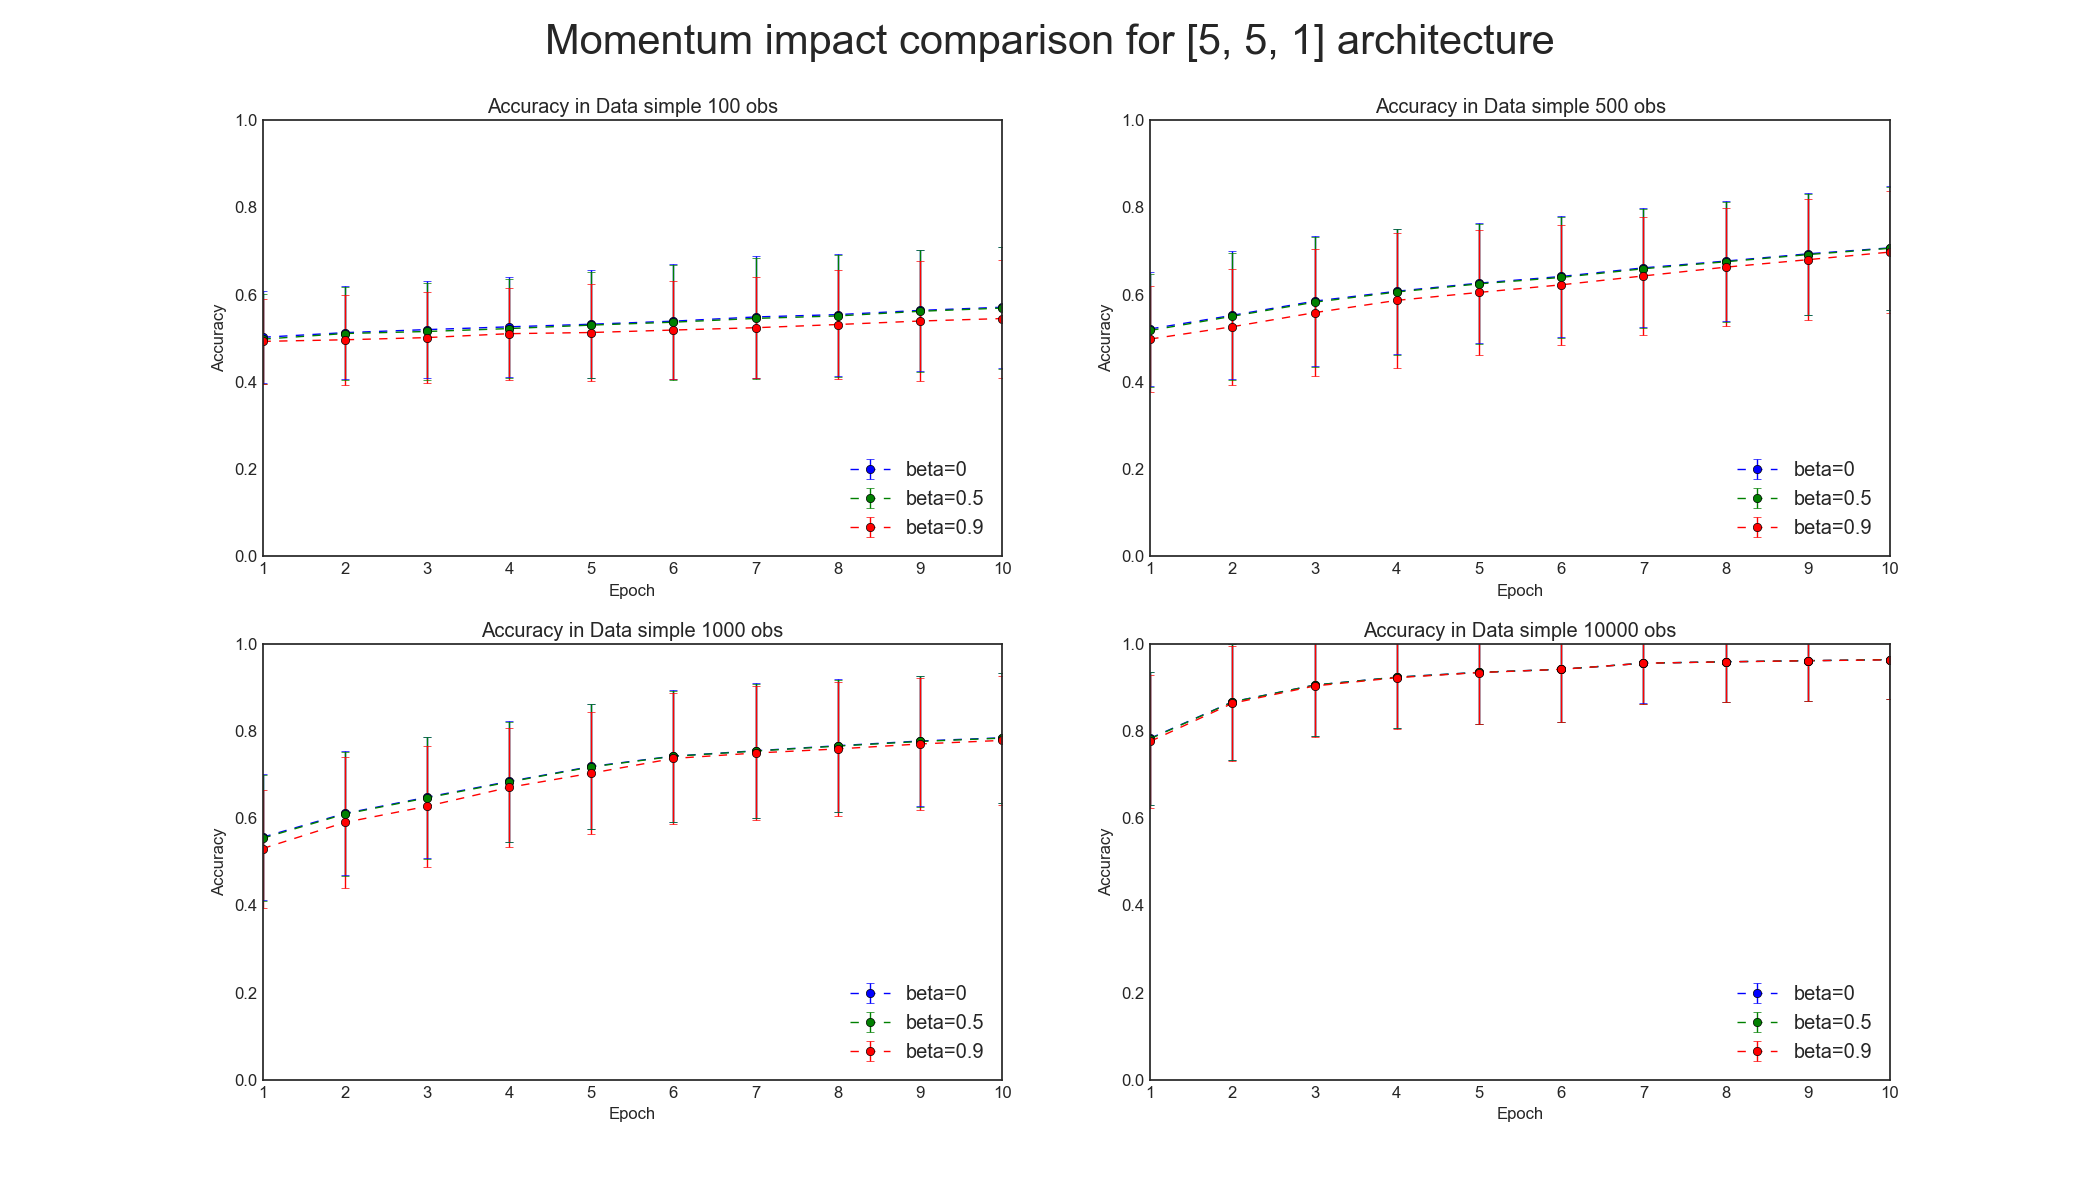
\includegraphics[width=1.4\textwidth]{results/classification/architecture-3/inertia_data_simple_2020_03_24_02_49_47.png}}
   \caption{Mean accuracy achieved on the test set.}
\end{figure}


\centerline{
\begin{tabular}{llll}
\hline
{} &        beta=0 &      beta=0.5 &      beta=0.9 \\
\hline
Data simple 100 obs   &  0.57 +- 0.14 &  0.57 +- 0.14 &  0.55 +- 0.14 \\
Data simple 500 obs   &  0.71 +- 0.14 &  0.71 +- 0.14 &  0.70 +- 0.14 \\
Data simple 1000 obs  &  0.78 +- 0.15 &  0.78 +- 0.15 &  0.78 +- 0.15 \\
Data simple 10000 obs &  0.96 +- 0.09 &  0.96 +- 0.09 &  0.96 +- 0.09 \\
\hline
\end{tabular}
}

\newpage
% ----------------- BS ACTIVATION DATA  -------------------------
\begin{figure}[!ht]
    \noindent\makebox[\textwidth]{%
   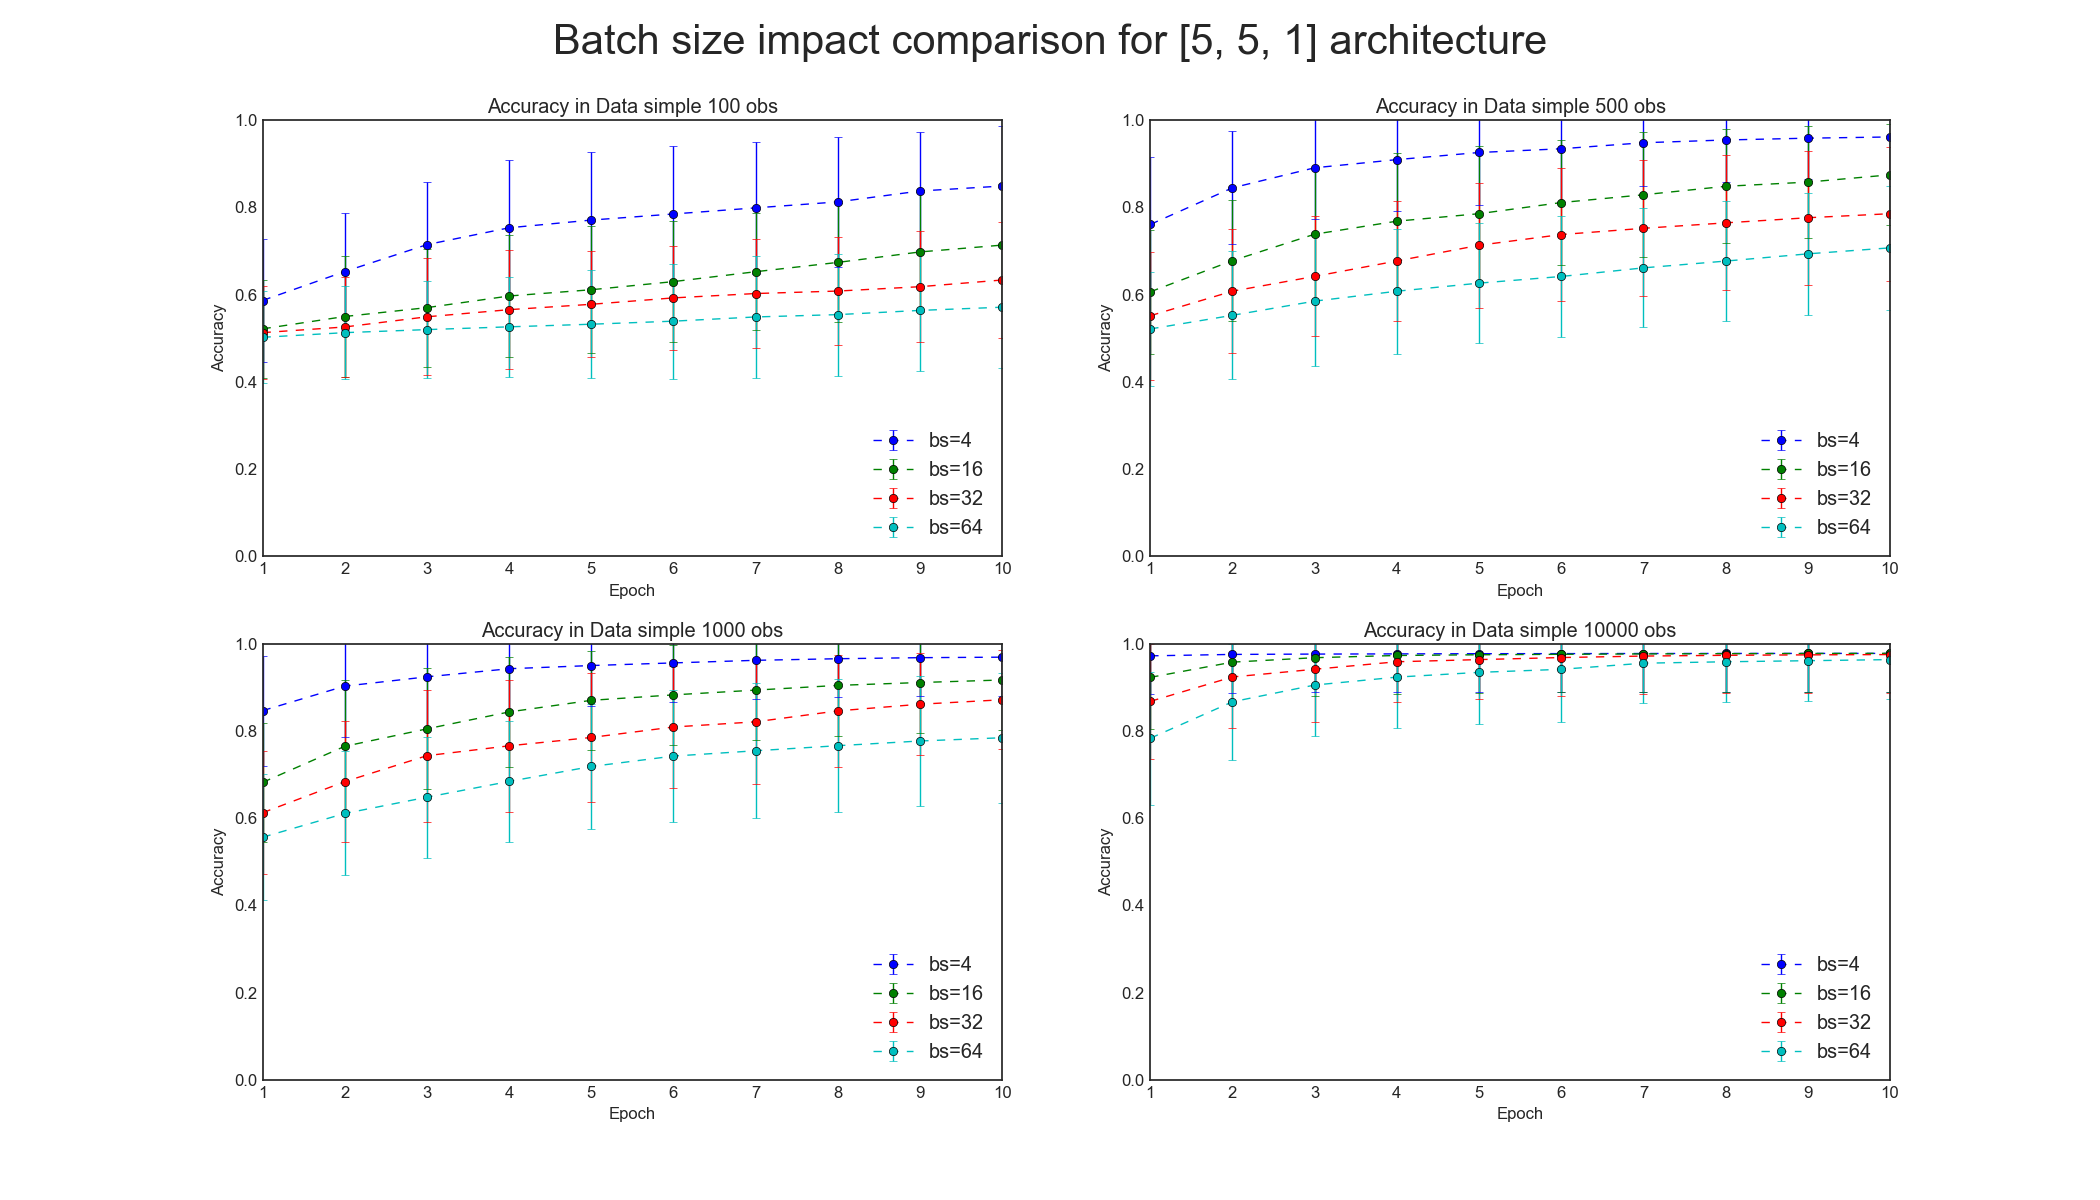
\includegraphics[width=1.4\textwidth]{results/classification/architecture-3/batch_size_data_simple_2020_03_24_02_49_47.png}}
   \caption{Mean accuracy achieved on the test set.}
\end{figure}

\centerline{
\begin{tabular}{lllll}
\hline
{} &          bs=4 &         bs=16 &         bs=32 &         bs=64 \\
\hline
Data simple 100 obs   &  0.85 +- 0.14 &  0.71 +- 0.14 &  0.63 +- 0.13 &  0.57 +- 0.14 \\
Data simple 500 obs   &  0.96 +- 0.09 &  0.87 +- 0.12 &  0.79 +- 0.15 &  0.71 +- 0.14 \\
Data simple 1000 obs  &  0.97 +- 0.09 &  0.92 +- 0.12 &  0.87 +- 0.11 &  0.78 +- 0.15 \\
Data simple 10000 obs &  0.98 +- 0.09 &  0.98 +- 0.09 &  0.97 +- 0.09 &  0.96 +- 0.09 \\
\hline
\end{tabular}
}

\newpage
\subsubsection{Architecture 4}
\[[10, 5]\]
Two hidden layers, first with 10 neurons, second with 5 neurons.

% ----------------- LR ACTIVATION DATA  -------------------------

\begin{figure}[!ht]
    \noindent\makebox[\textwidth]{%
   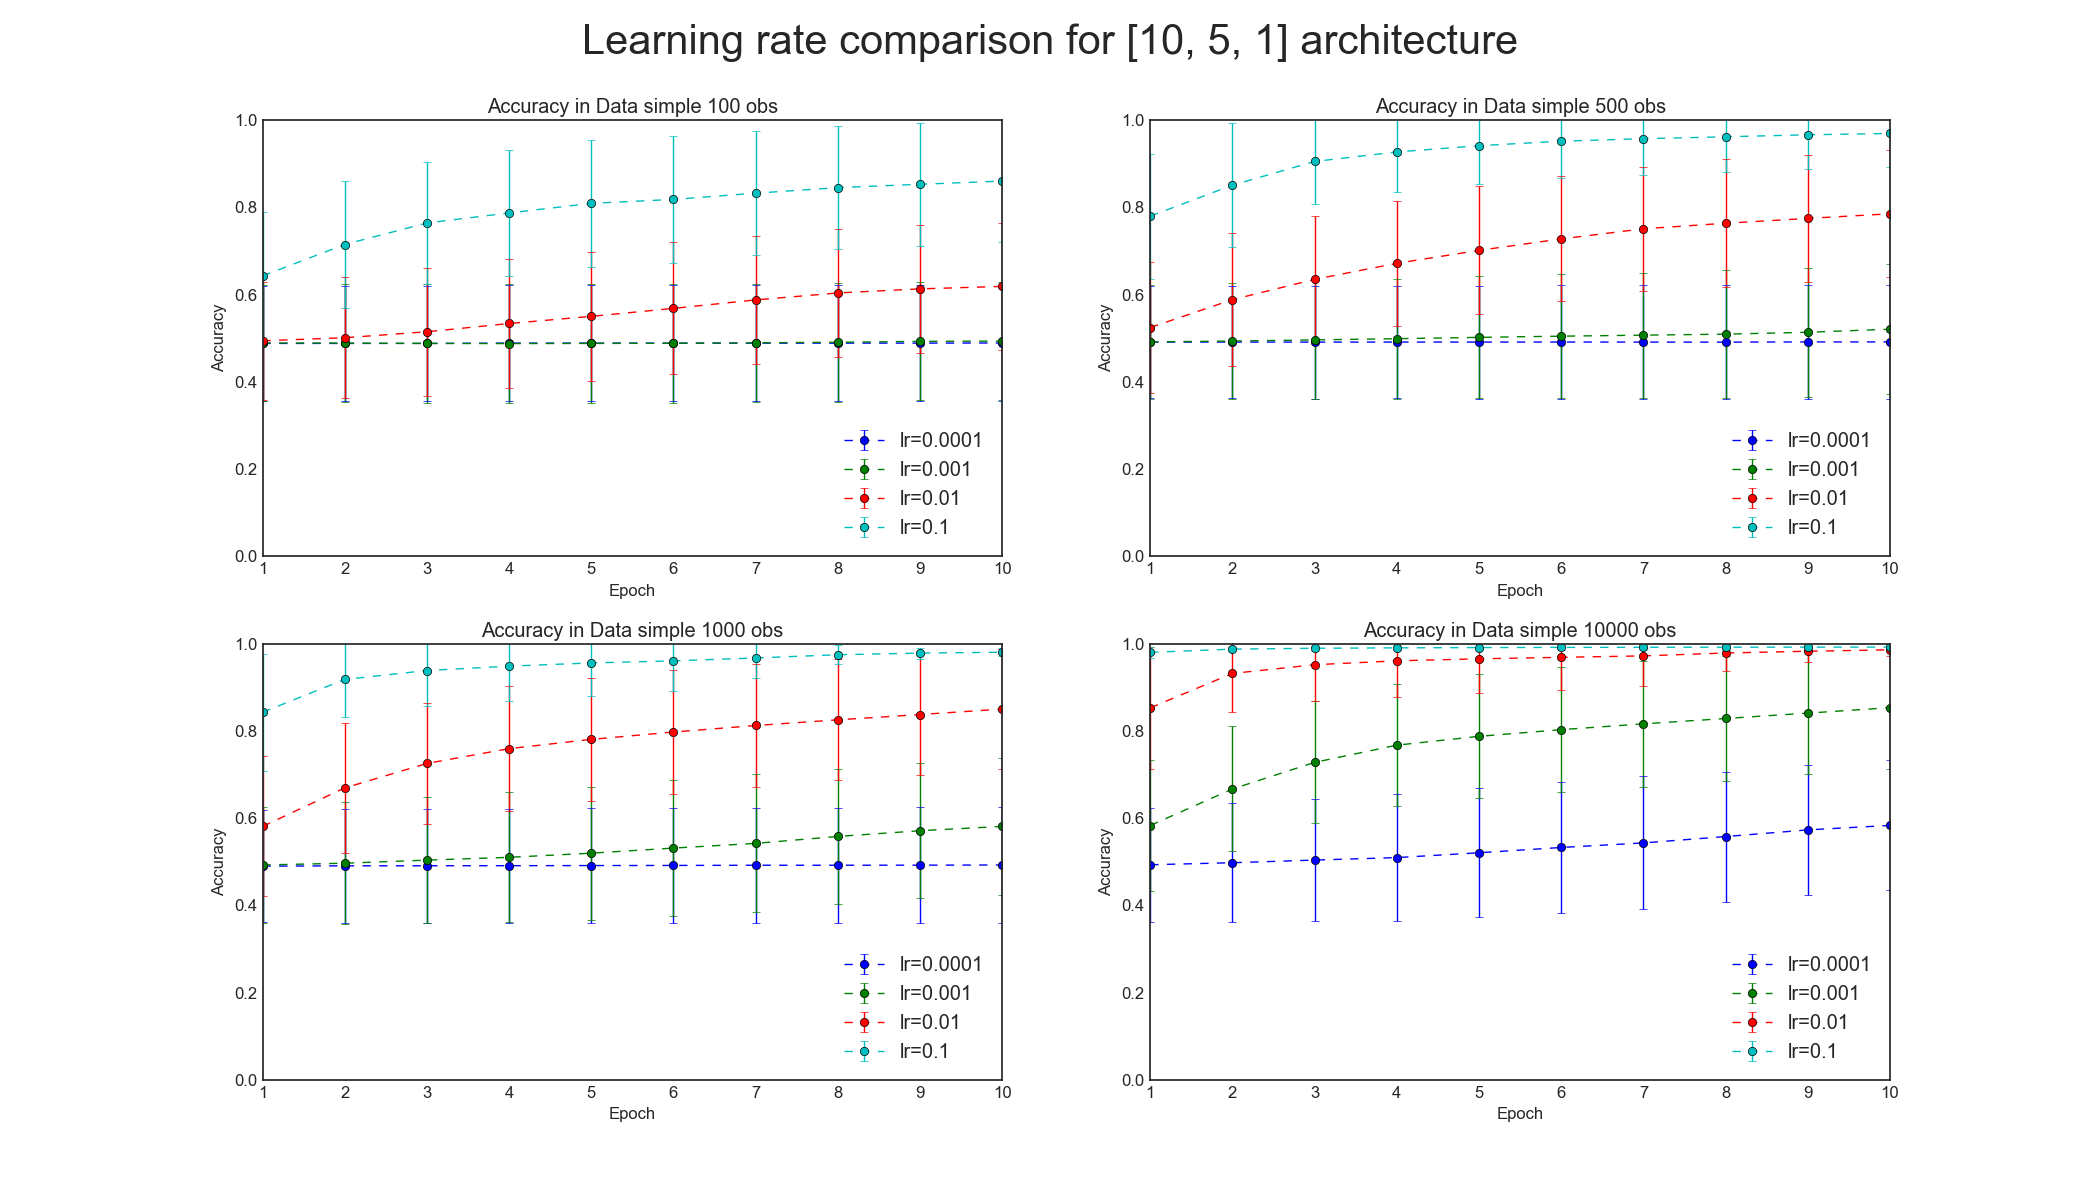
\includegraphics[width=1.4\textwidth]{results/classification/architecture-4/lr_data_simple_2020_03_24_02_57_46.png}}
   \caption{Mean accuracy achieved on the test set.}
\end{figure}

\centerline{
\begin{tabular}{lllll}
\hline
{} &     lr=0.0001 &      lr=0.001 &       lr=0.01 &        lr=0.1 \\
\hline
Data simple 100 obs   &  0.49 +- 0.13 &  0.49 +- 0.14 &  0.62 +- 0.15 &  0.86 +- 0.14 \\
Data simple 500 obs   &  0.49 +- 0.13 &  0.52 +- 0.15 &  0.79 +- 0.15 &  0.97 +- 0.08 \\
Data simple 1000 obs  &  0.49 +- 0.13 &  0.58 +- 0.16 &  0.85 +- 0.14 &  0.98 +- 0.01 \\
Data simple 10000 obs &  0.58 +- 0.15 &  0.85 +- 0.14 &  0.99 +- 0.01 &  0.99 +- 0.01 \\
\hline
\end{tabular}
}

\newpage
% ----------------- AF ACTIVATION DATA  -------------------------
\begin{figure}[!ht]
    \noindent\makebox[\textwidth]{%
   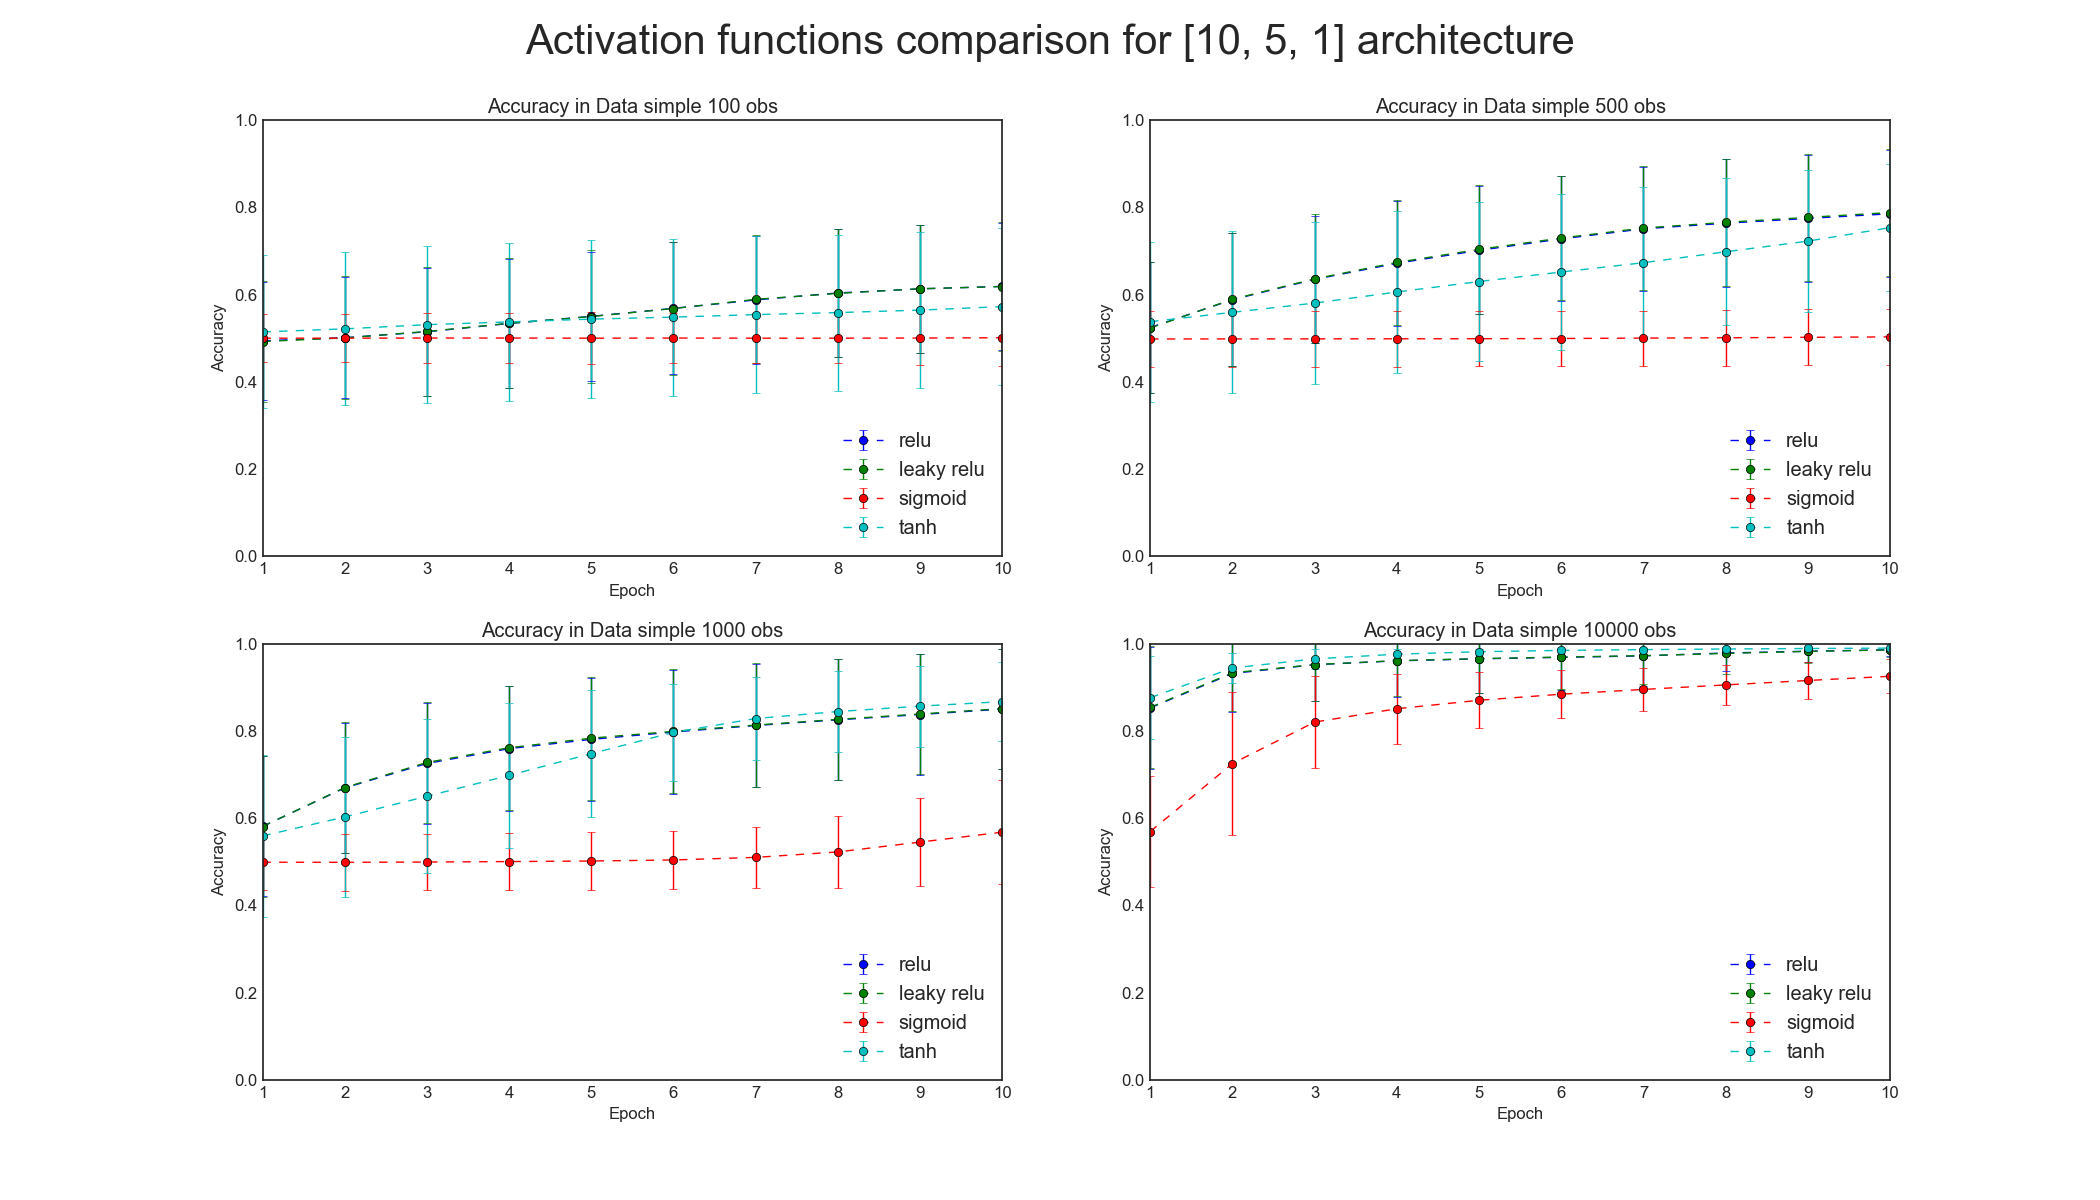
\includegraphics[width=1.4\textwidth]{results/classification/architecture-4/activation_function_data_simple_2020_03_24_02_57_46.png}}
   \caption{Mean accuracy achieved on the test set.}
\end{figure}


\centerline{
\begin{tabular}{lllll}
\hline
{} &          relu &    leaky relu &       sigmoid &          tanh \\
\hline
Data simple 100 obs   &  0.62 +- 0.15 &  0.62 +- 0.15 &  0.50 +- 0.07 &  0.57 +- 0.18 \\
Data simple 500 obs   &  0.79 +- 0.15 &  0.79 +- 0.14 &  0.50 +- 0.06 &  0.75 +- 0.15 \\
Data simple 1000 obs  &  0.85 +- 0.14 &  0.85 +- 0.14 &  0.57 +- 0.12 &  0.87 +- 0.09 \\
Data simple 10000 obs &  0.99 +- 0.01 &  0.99 +- 0.02 &  0.93 +- 0.04 &  0.99 +- 0.00 \\
\hline
\end{tabular}
}

\newpage
% ----------------- INERTIA ACTIVATION DATA  -------------------------
\begin{figure}[!ht]
    \noindent\makebox[\textwidth]{%
   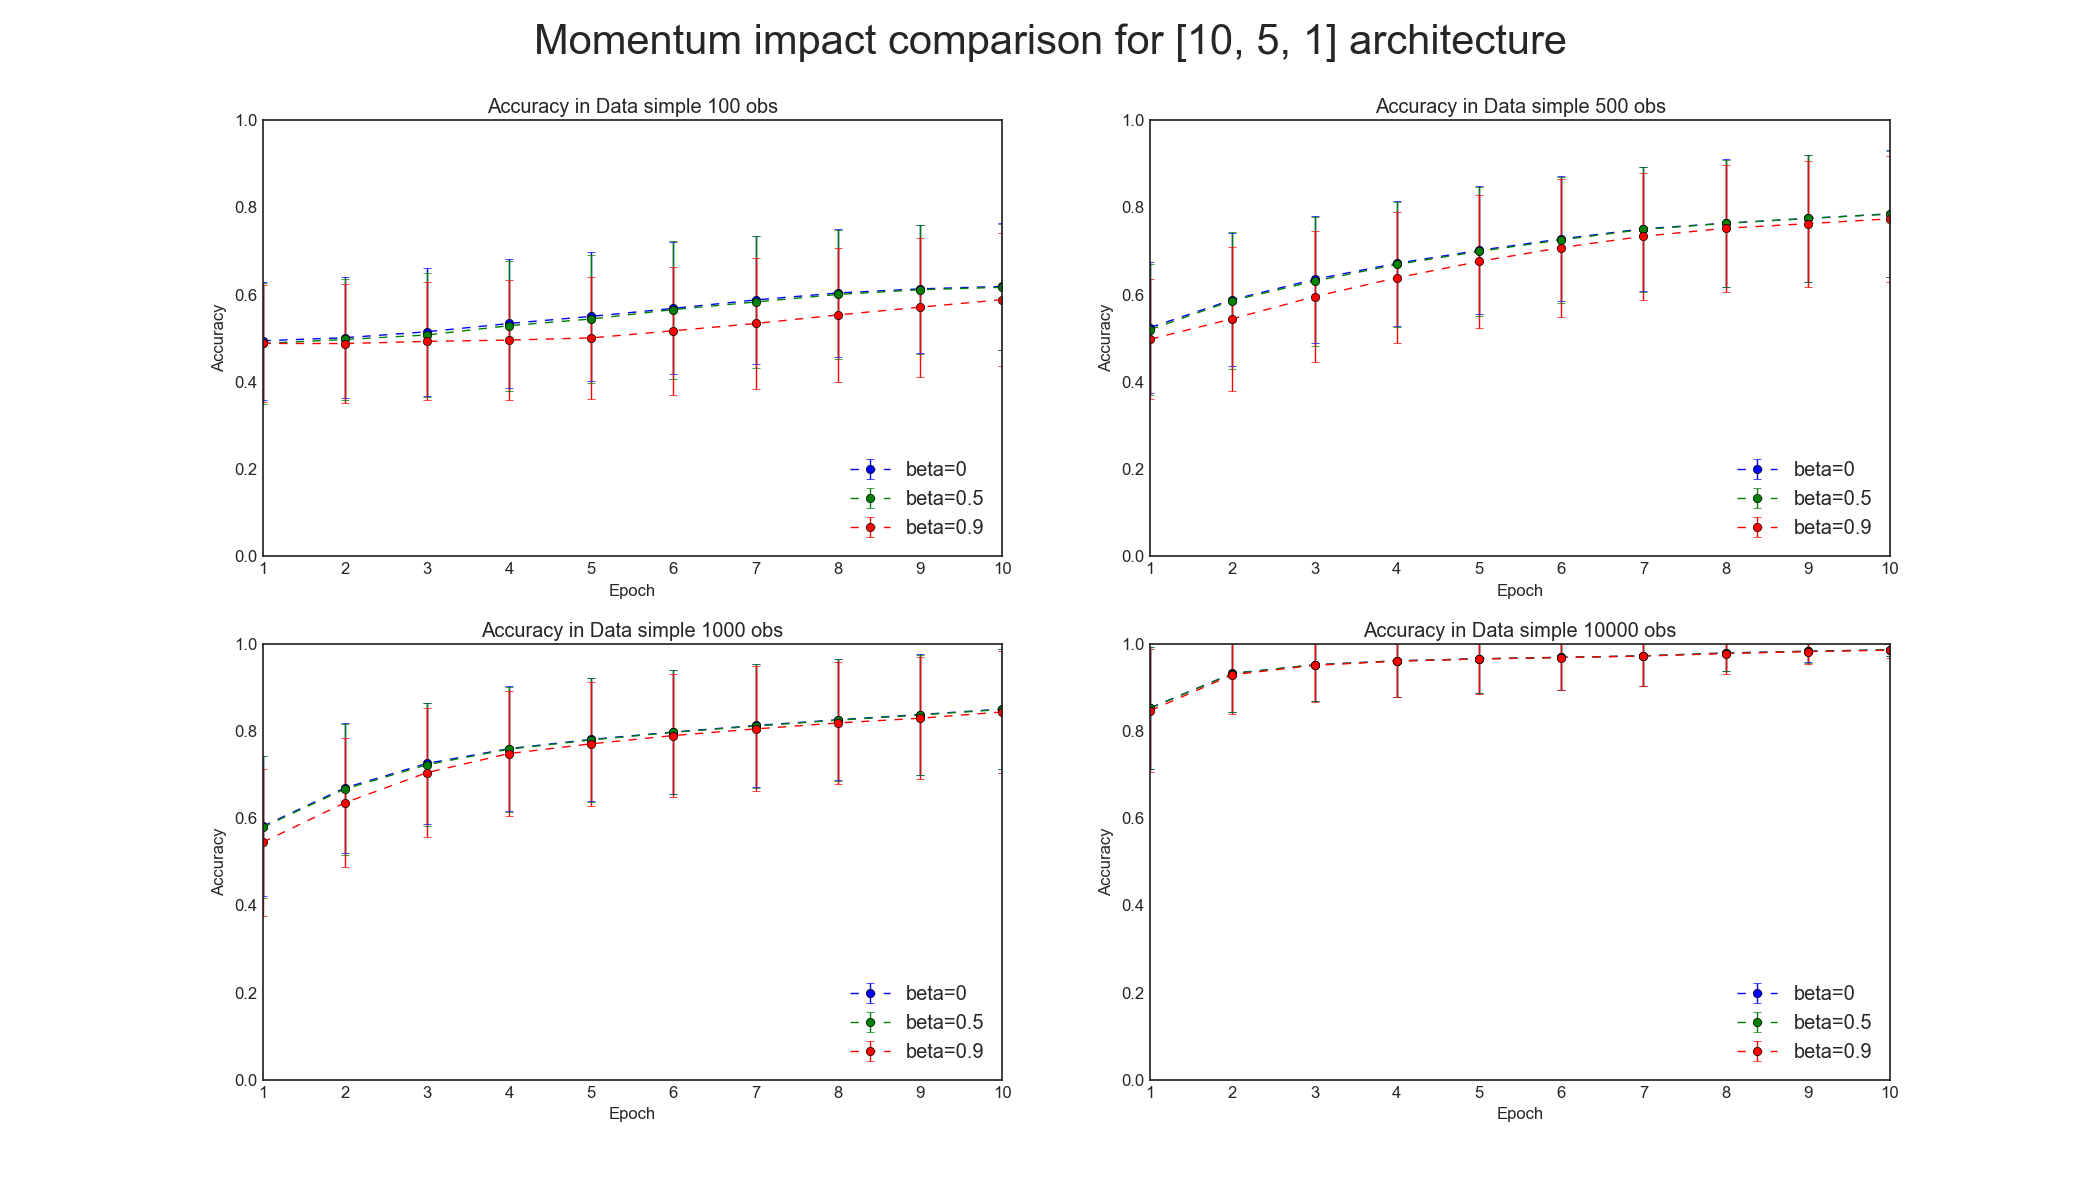
\includegraphics[width=1.4\textwidth]{results/classification/architecture-4/inertia_data_simple_2020_03_24_02_57_47.png}}
   \caption{Mean accuracy achieved on the test set.}
\end{figure}


\centerline{
\begin{tabular}{llll}
\hline
{} &        beta=0 &      beta=0.5 &      beta=0.9 \\
\hline
Data simple 100 obs   &  0.62 +- 0.15 &  0.62 +- 0.14 &  0.59 +- 0.15 \\
Data simple 500 obs   &  0.79 +- 0.15 &  0.78 +- 0.15 &  0.77 +- 0.14 \\
Data simple 1000 obs  &  0.85 +- 0.14 &  0.85 +- 0.14 &  0.84 +- 0.14 \\
Data simple 10000 obs &  0.99 +- 0.01 &  0.99 +- 0.01 &  0.98 +- 0.02 \\
\hline
\end{tabular}
}

\newpage
% ----------------- BS ACTIVATION DATA  -------------------------
\begin{figure}[!ht]
    \noindent\makebox[\textwidth]{%
   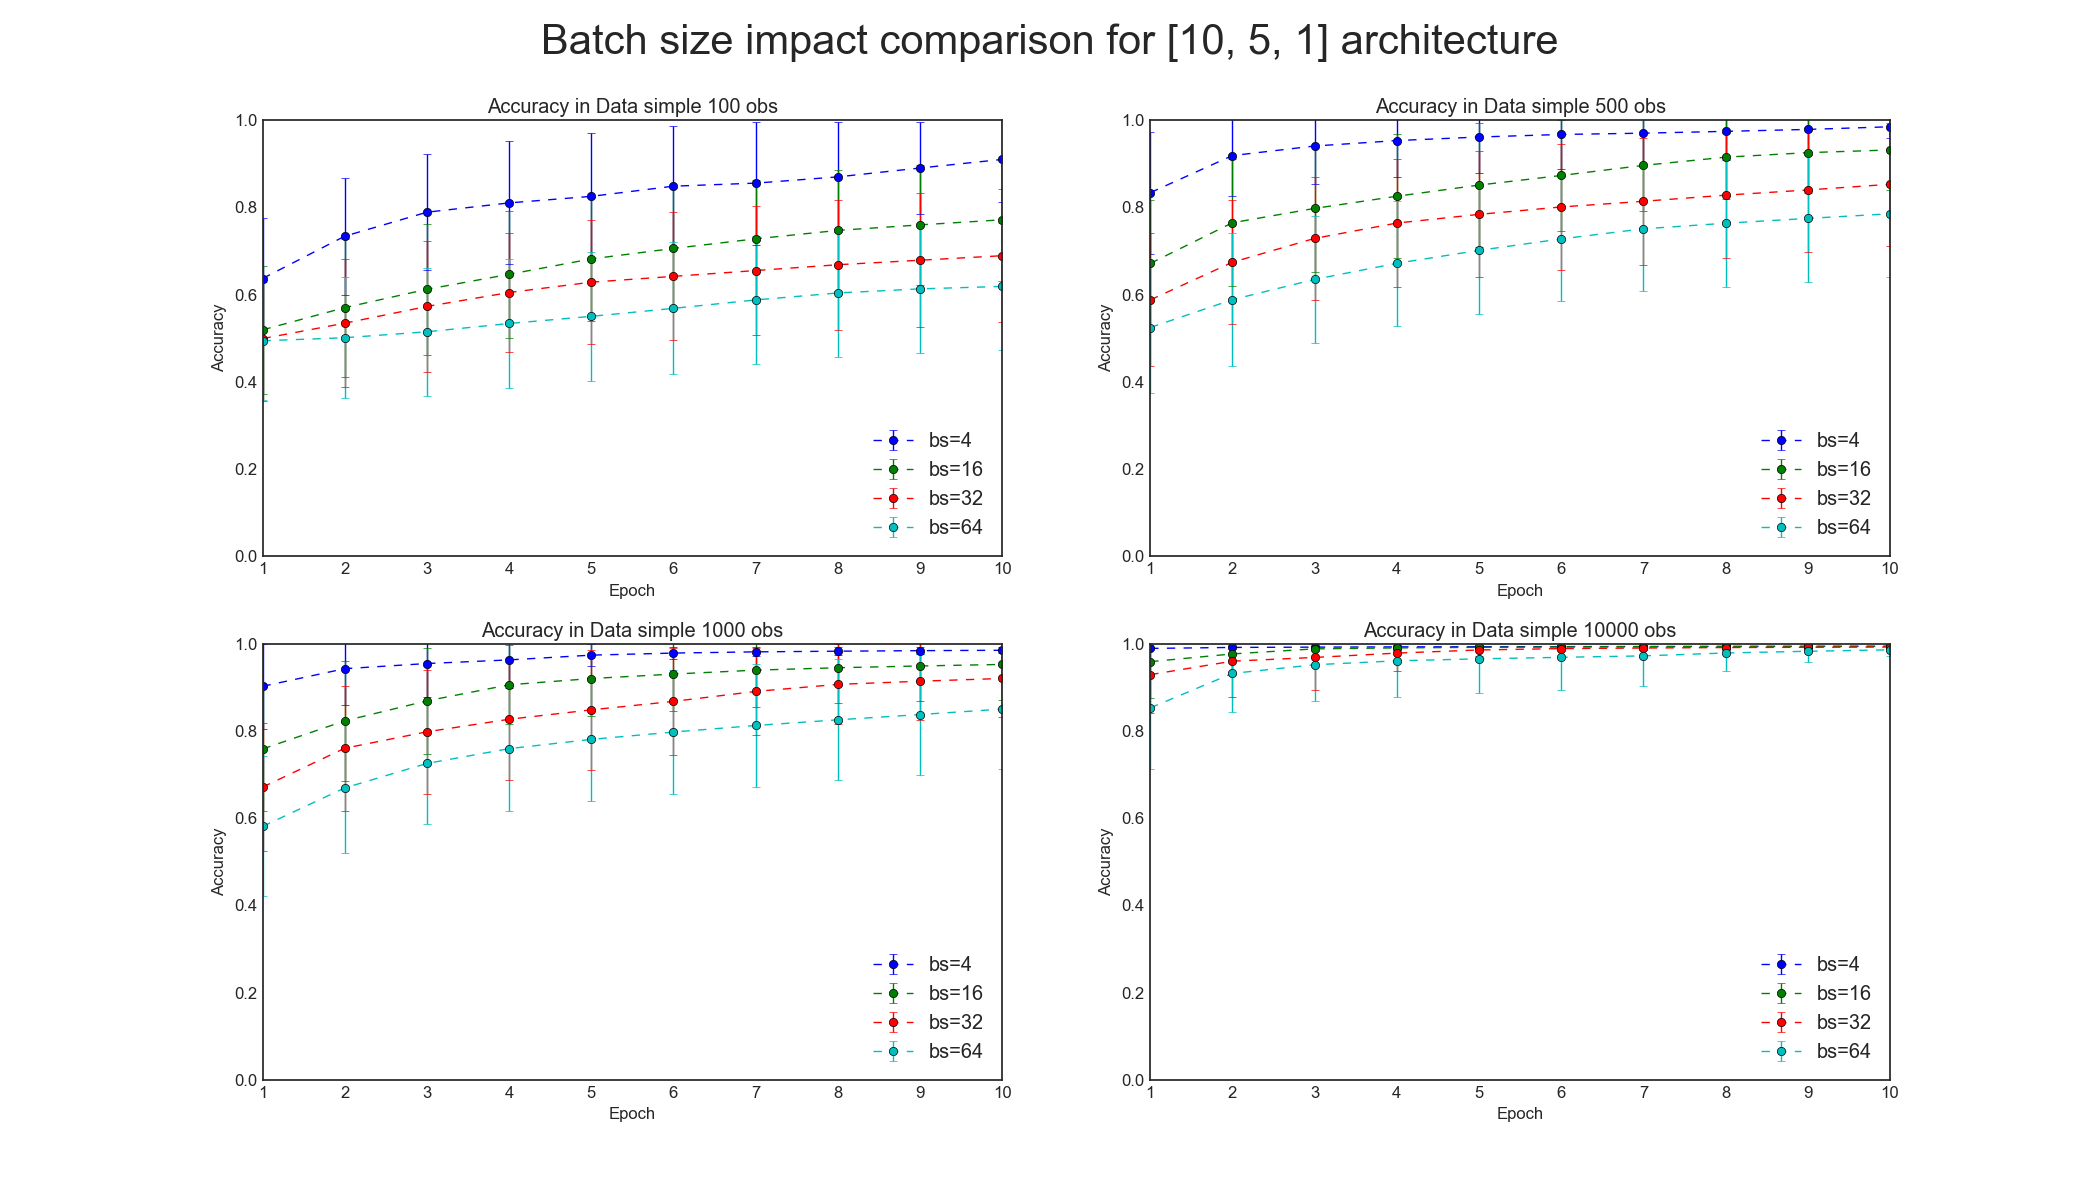
\includegraphics[width=1.4\textwidth]{results/classification/architecture-4/batch_size_data_simple_2020_03_24_02_57_47.png}}
   \caption{Mean accuracy achieved on the test set.}
\end{figure}

\centerline{
\begin{tabular}{lllll}
\hline
{} &          bs=4 &         bs=16 &         bs=32 &         bs=64 \\
\hline
Data simple 100 obs   &  0.91 +- 0.10 &  0.77 +- 0.14 &  0.69 +- 0.15 &  0.62 +- 0.15 \\
Data simple 500 obs   &  0.98 +- 0.03 &  0.93 +- 0.09 &  0.85 +- 0.14 &  0.79 +- 0.15 \\
Data simple 1000 obs  &  0.98 +- 0.01 &  0.95 +- 0.08 &  0.92 +- 0.09 &  0.85 +- 0.14 \\
Data simple 10000 obs &  0.99 +- 0.00 &  0.99 +- 0.00 &  0.99 +- 0.00 &  0.99 +- 0.01 \\
\hline
\end{tabular}
}

\newpage
\subsubsection{Architecture 5}
\[[5, 5, 5, 5]\]
Four hidden layers, each with 5 neurons.

% ----------------- LR ACTIVATION DATA  -------------------------

\begin{figure}[!ht]
    \noindent\makebox[\textwidth]{%
   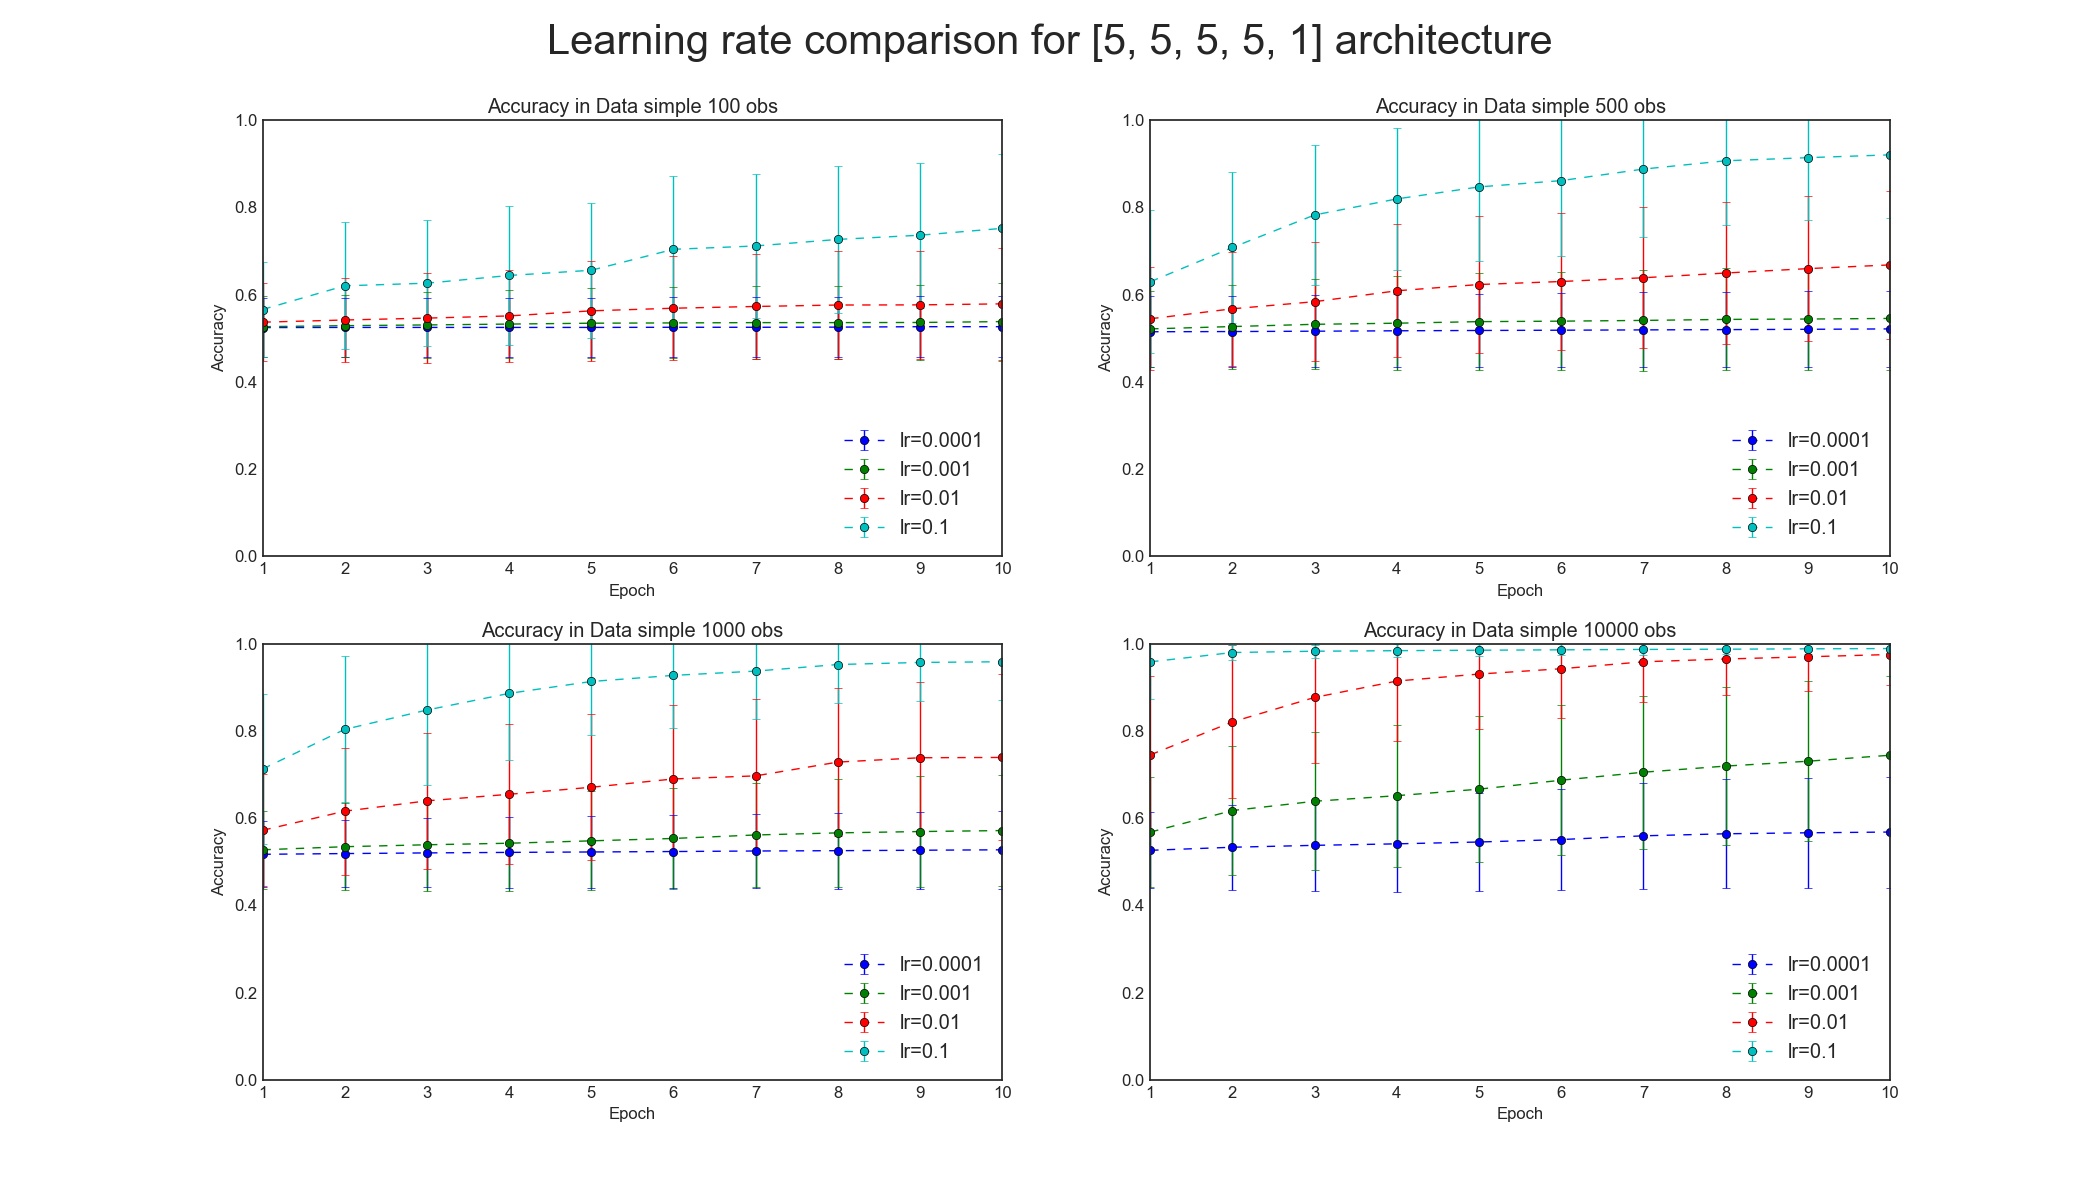
\includegraphics[width=1.4\textwidth]{results/classification/architecture-5/lr_data_simple_2020_03_24_03_07_28.png}}
   \caption{Mean accuracy achieved on the test set.}
\end{figure}

\centerline{
\begin{tabular}{lllll}
\hline
{} &     lr=0.0001 &      lr=0.001 &       lr=0.01 &        lr=0.1 \\
\hline
Data simple 100 obs   &  0.53 +- 0.07 &  0.54 +- 0.09 &  0.58 +- 0.13 &  0.75 +- 0.17 \\
Data simple 500 obs   &  0.52 +- 0.09 &  0.55 +- 0.12 &  0.67 +- 0.17 &  0.92 +- 0.14 \\
Data simple 1000 obs  &  0.53 +- 0.09 &  0.57 +- 0.13 &  0.74 +- 0.19 &  0.96 +- 0.09 \\
Data simple 10000 obs &  0.57 +- 0.13 &  0.74 +- 0.18 &  0.98 +- 0.07 &  0.99 +- 0.01 \\
\hline
\end{tabular}
}

\newpage
% ----------------- AF ACTIVATION DATA  -------------------------
\begin{figure}[!ht]
    \noindent\makebox[\textwidth]{%
   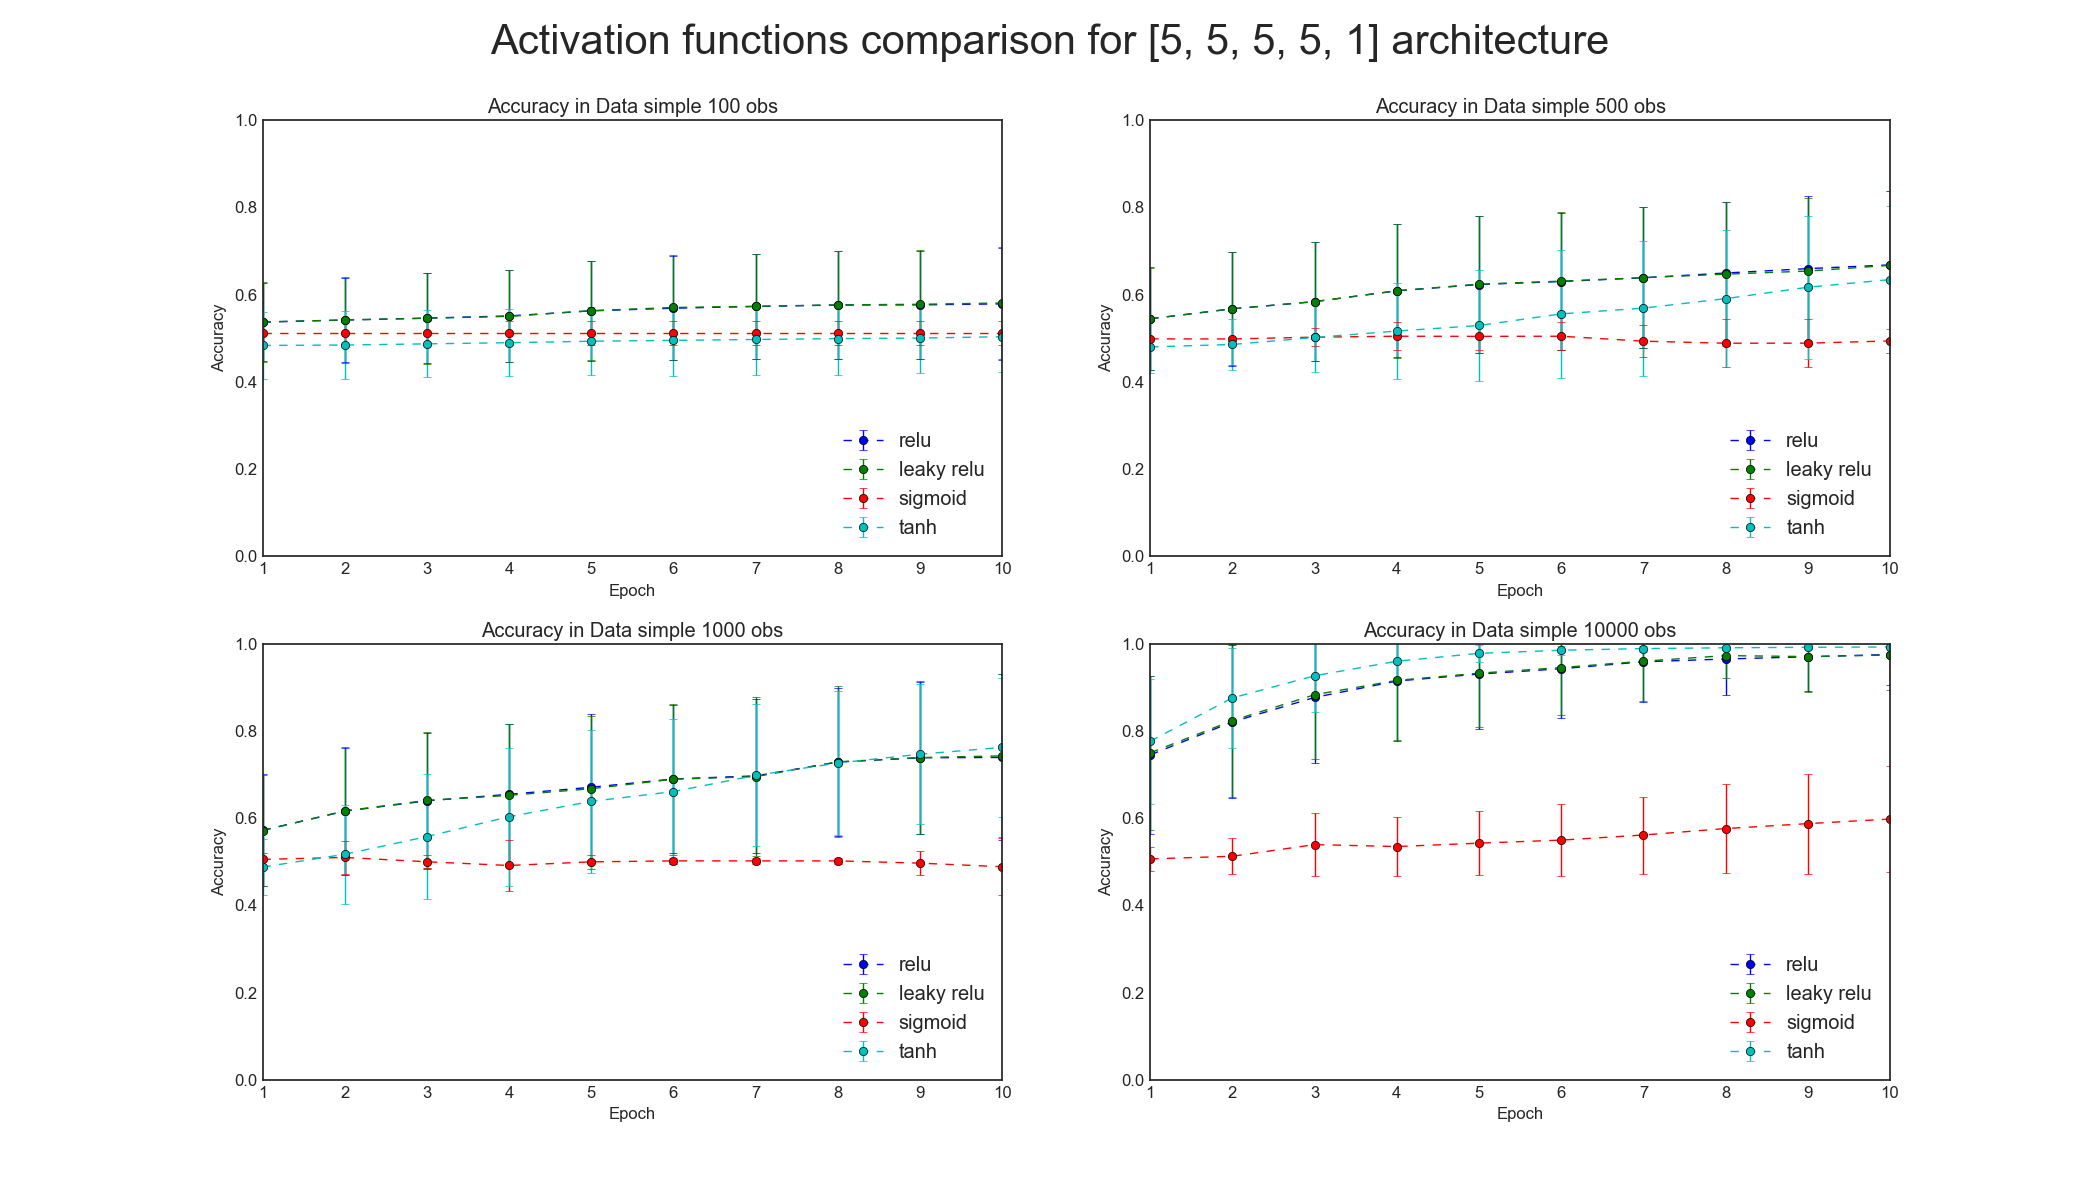
\includegraphics[width=1.4\textwidth]{results/classification/architecture-5/activation_function_data_simple_2020_03_24_03_07_28.png}}
   \caption{Mean accuracy achieved on the test set.}
\end{figure}


\centerline{
\begin{tabular}{lllll}
\hline
{} &          relu &    leaky relu &       sigmoid &          tanh \\
\hline
Data simple 100 obs   &  0.58 +- 0.13 &  0.58 +- 0.13 &  0.51 +- 0.03 &  0.50 +- 0.08 \\
Data simple 500 obs   &  0.67 +- 0.17 &  0.67 +- 0.17 &  0.50 +- 0.03 &  0.63 +- 0.17 \\
Data simple 1000 obs  &  0.74 +- 0.19 &  0.74 +- 0.19 &  0.51 +- 0.04 &  0.76 +- 0.16 \\
Data simple 10000 obs &  0.98 +- 0.07 &  0.97 +- 0.08 &  0.60 +- 0.12 &  0.99 +- 0.00 \\
\hline
\end{tabular}
}


\newpage
% ----------------- INERTIA ACTIVATION DATA  -------------------------
\begin{figure}[!ht]
    \noindent\makebox[\textwidth]{%
   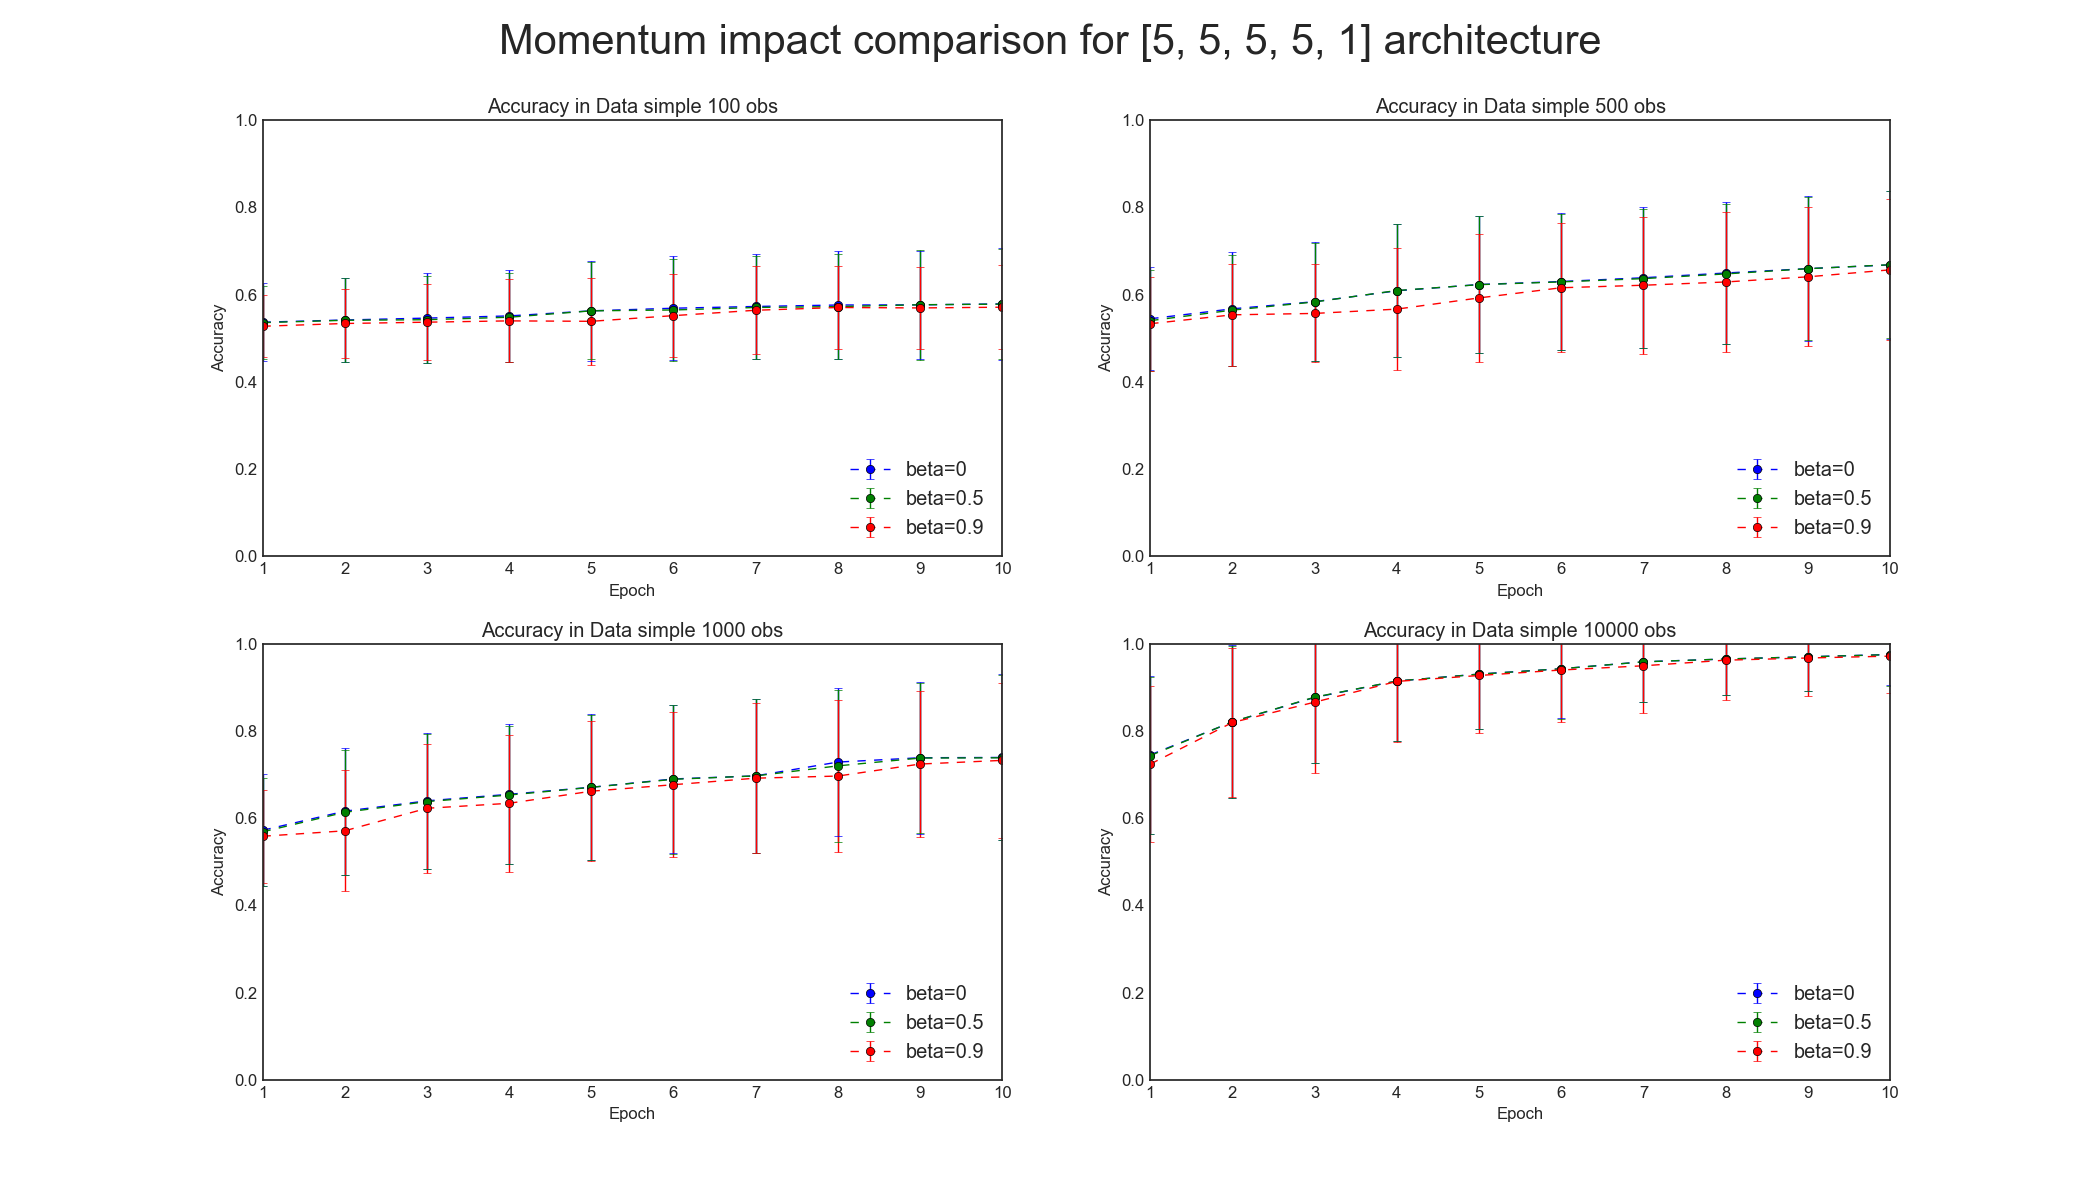
\includegraphics[width=1.4\textwidth]{results/classification/architecture-5/inertia_data_simple_2020_03_24_03_07_28.png}}
   \caption{Mean accuracy achieved on the test set.}
\end{figure}


\centerline{
\begin{tabular}{llll}
\hline
{} &        beta=0 &      beta=0.5 &      beta=0.9 \\
\hline
Data simple 100 obs   &  0.58 +- 0.13 &  0.58 +- 0.13 &  0.57 +- 0.10 \\
Data simple 500 obs   &  0.67 +- 0.17 &  0.67 +- 0.17 &  0.66 +- 0.16 \\
Data simple 1000 obs  &  0.74 +- 0.19 &  0.74 +- 0.19 &  0.73 +- 0.18 \\
Data simple 10000 obs &  0.98 +- 0.07 &  0.97 +- 0.07 &  0.97 +- 0.08 \\
\hline
\end{tabular}
}

\newpage
% ----------------- BS ACTIVATION DATA  -------------------------
\begin{figure}[!ht]
    \noindent\makebox[\textwidth]{%
   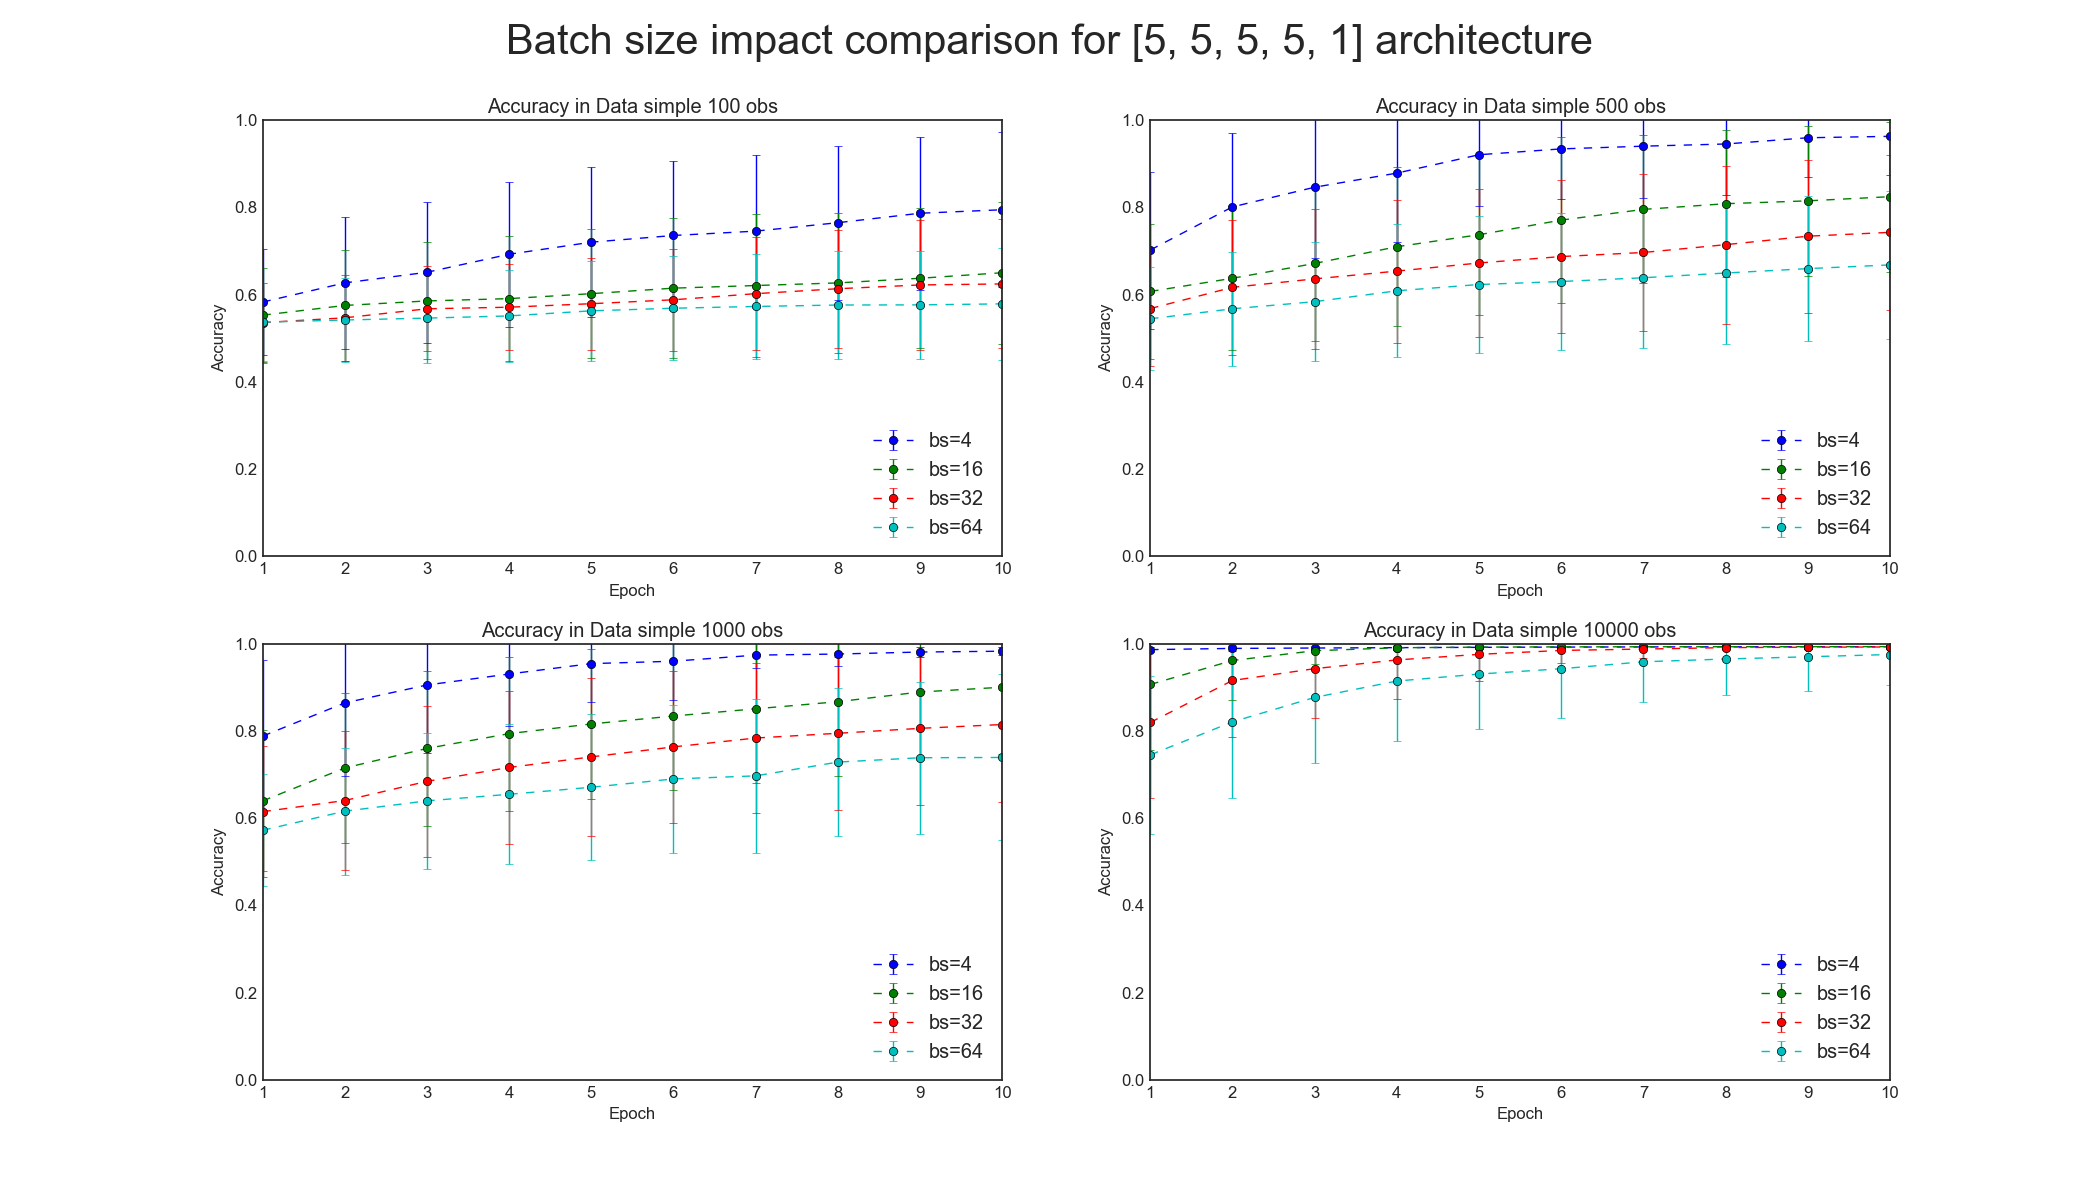
\includegraphics[width=1.4\textwidth]{results/classification/architecture-5/batch_size_data_simple_2020_03_24_03_07_29.png}}
   \caption{Mean accuracy achieved on the test set.}
\end{figure}

\centerline{
\begin{tabular}{lllll}
\hline
{} &          bs=4 &         bs=16 &         bs=32 &         bs=64 \\
\hline
Data simple 100 obs   &  0.79 +- 0.18 &  0.65 +- 0.16 &  0.62 +- 0.15 &  0.58 +- 0.13 \\
Data simple 500 obs   &  0.96 +- 0.09 &  0.82 +- 0.17 &  0.74 +- 0.18 &  0.67 +- 0.17 \\
Data simple 1000 obs  &  0.98 +- 0.01 &  0.90 +- 0.15 &  0.81 +- 0.18 &  0.74 +- 0.19 \\
Data simple 10000 obs &  0.99 +- 0.00 &  0.99 +- 0.00 &  0.99 +- 0.00 &  0.98 +- 0.07 \\
\hline
\end{tabular}
}

\newpage
\subsubsection{Architecture 6}
\[[10, 10, 5, 5]\]
Four hidden layers, first two with 10 neurons, second two with 5 neurons.

% ----------------- LR ACTIVATION DATA  -------------------------

\begin{figure}[!ht]
    \noindent\makebox[\textwidth]{%
   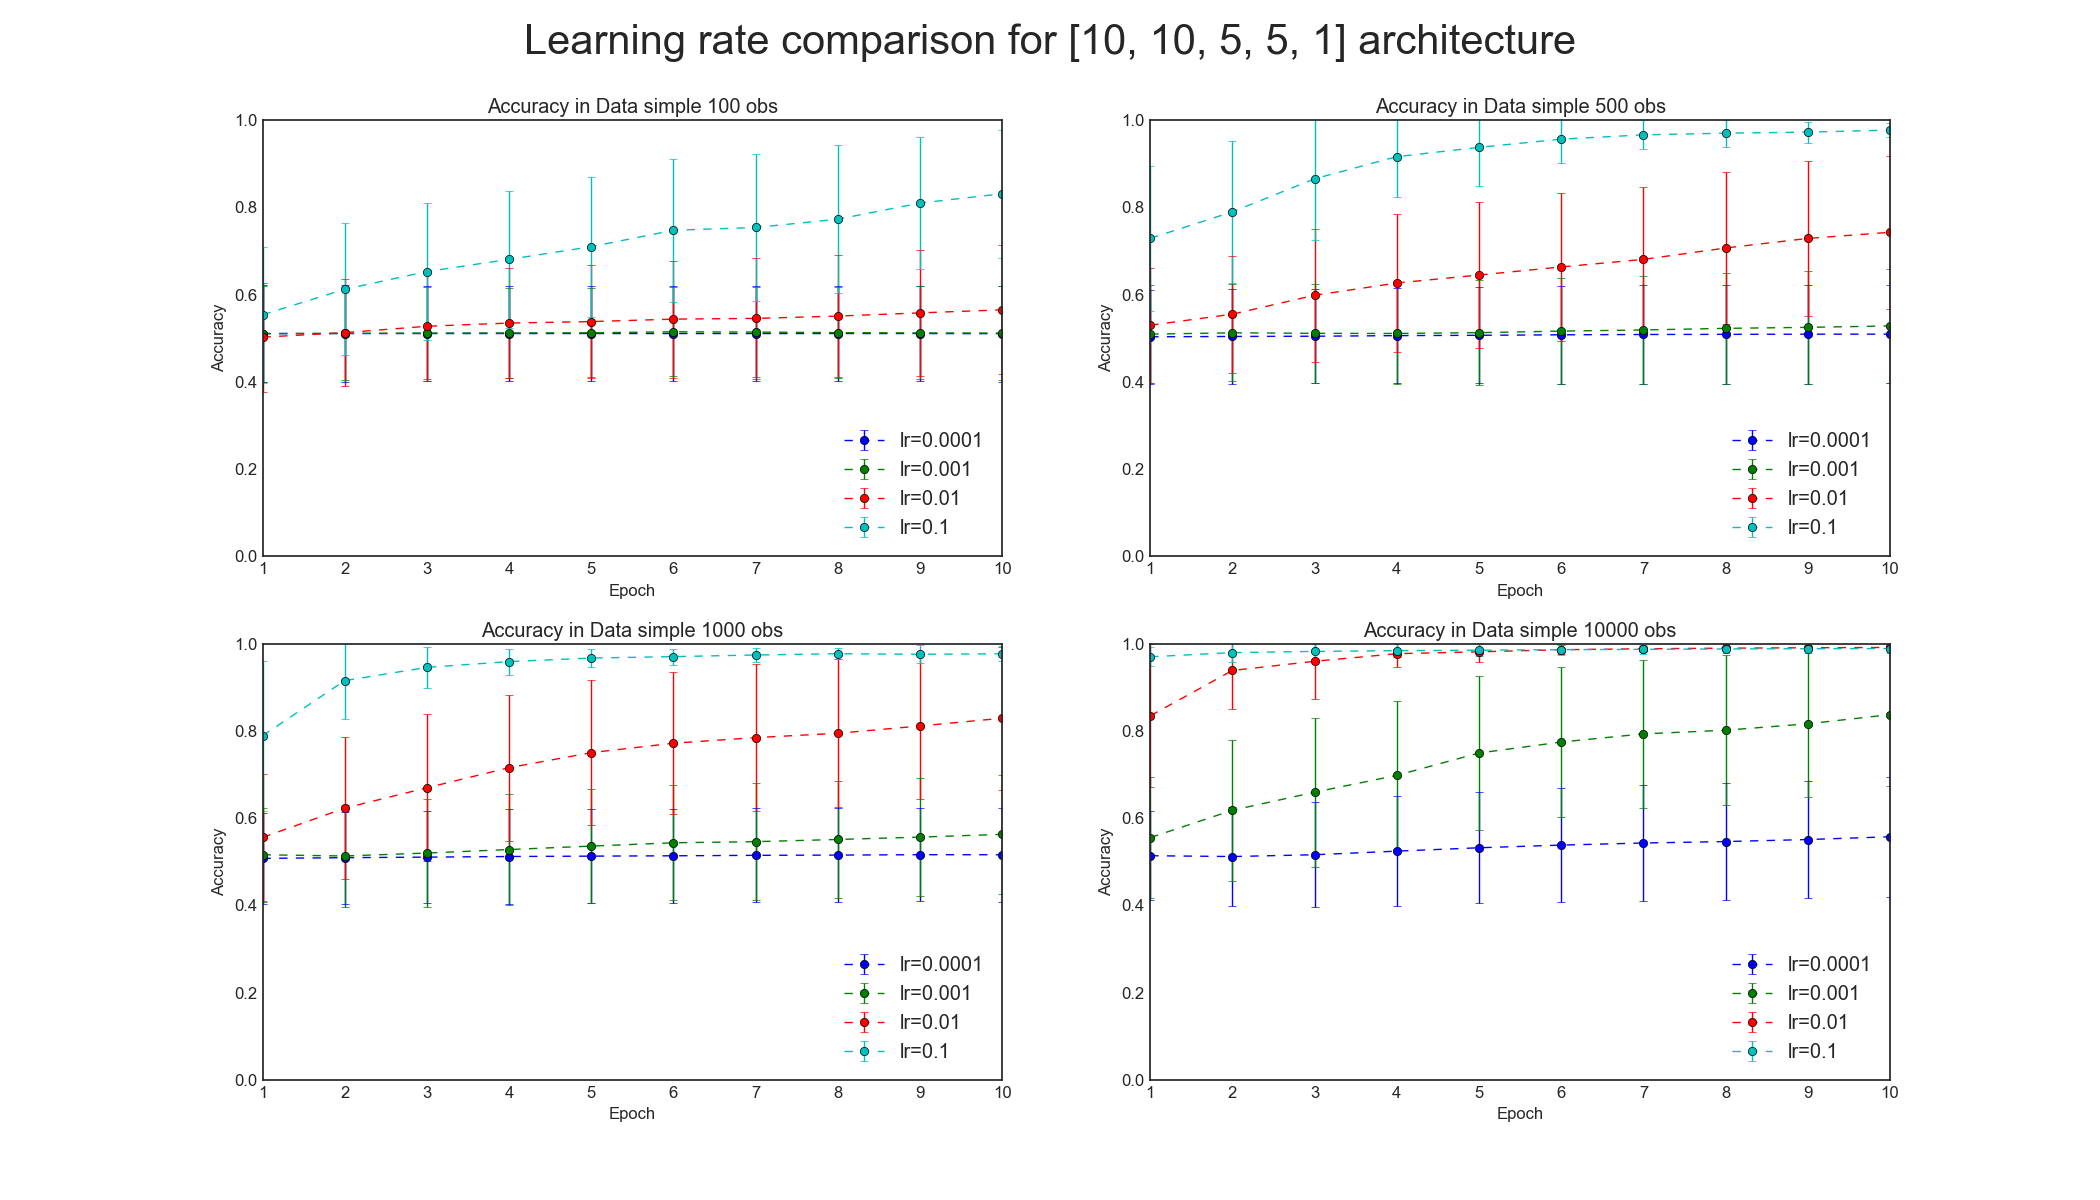
\includegraphics[width=1.4\textwidth]{results/classification/architecture-6/lr_data_simple_2020_03_24_03_17_18.png}}
   \caption{Mean accuracy achieved on the test set.}
\end{figure}

\centerline{
\begin{tabular}{lllll}
\hline
{} &     lr=0.0001 &      lr=0.001 &       lr=0.01 &        lr=0.1 \\
\hline
Data simple 100 obs   &  0.51 +- 0.11 &  0.51 +- 0.10 &  0.56 +- 0.15 &  0.83 +- 0.15 \\
Data simple 500 obs   &  0.51 +- 0.11 &  0.53 +- 0.13 &  0.74 +- 0.18 &  0.98 +- 0.02 \\
Data simple 1000 obs  &  0.52 +- 0.11 &  0.56 +- 0.14 &  0.83 +- 0.16 &  0.98 +- 0.01 \\
Data simple 10000 obs &  0.56 +- 0.14 &  0.84 +- 0.16 &  0.99 +- 0.00 &  0.99 +- 0.01 \\
\hline
\end{tabular}
}

\newpage
% ----------------- AF ACTIVATION DATA  -------------------------
\begin{figure}[!ht]
    \noindent\makebox[\textwidth]{%
   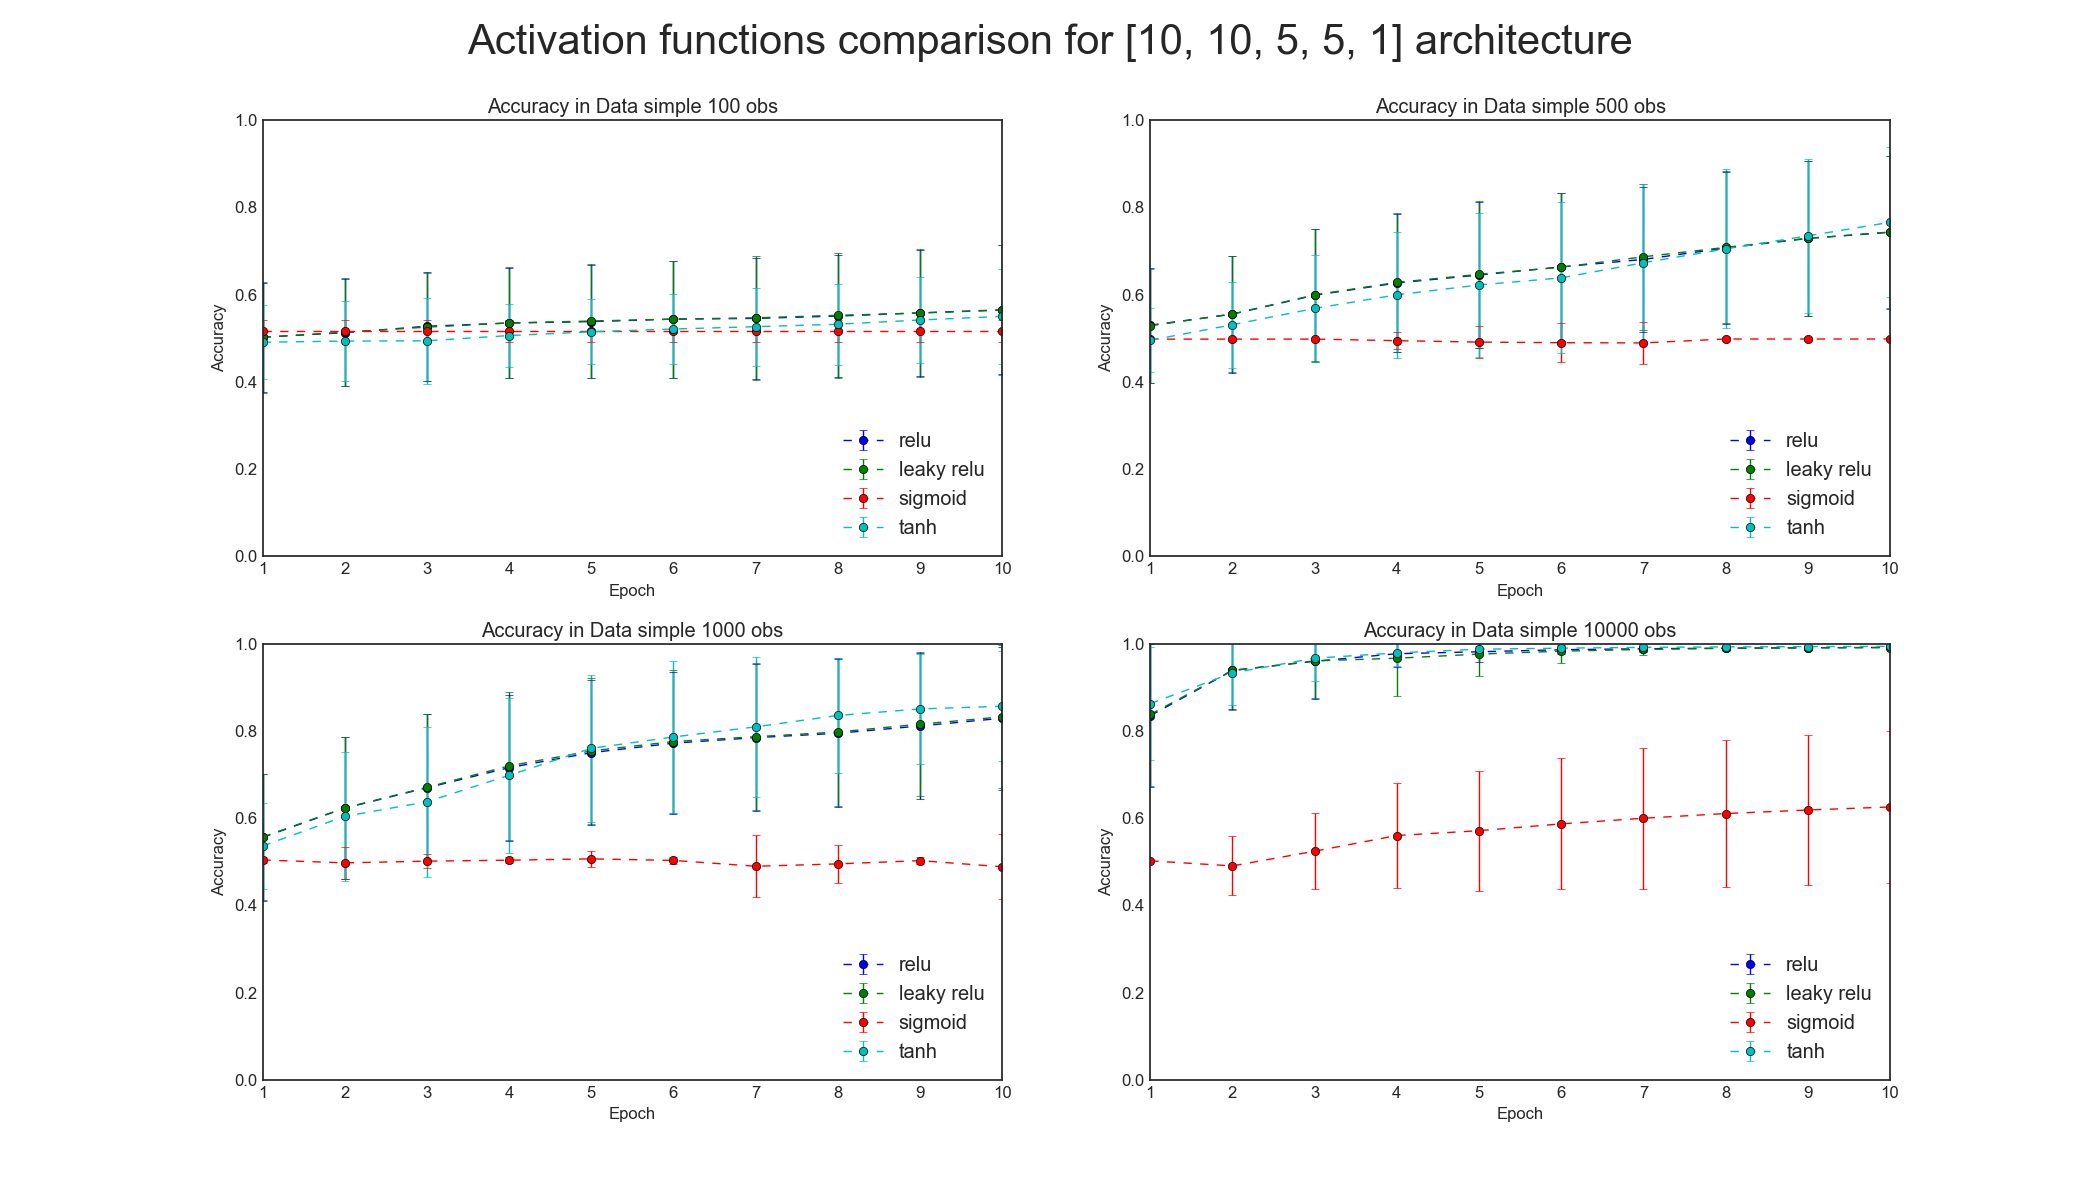
\includegraphics[width=1.4\textwidth]{results/classification/architecture-6/activation_function_data_simple_2020_03_24_03_17_19.png}}
   \caption{Mean accuracy achieved on the test set.}
\end{figure}


\centerline{
\begin{tabular}{lllll}
\hline
{} &          relu &    leaky relu &       sigmoid &          tanh \\
\hline
Data simple 100 obs   &  0.56 +- 0.15 &  0.56 +- 0.15 &  0.52 +- 0.03 &  0.55 +- 0.11 \\
Data simple 500 obs   &  0.74 +- 0.18 &  0.74 +- 0.17 &  0.50 +- 0.00 &  0.77 +- 0.17 \\
Data simple 1000 obs  &  0.83 +- 0.16 &  0.83 +- 0.16 &  0.51 +- 0.02 &  0.86 +- 0.13 \\
Data simple 10000 obs &  0.99 +- 0.00 &  0.99 +- 0.00 &  0.63 +- 0.17 &  0.99 +- 0.00 \\
\hline
\end{tabular}
}

\newpage
% ----------------- INERTIA ACTIVATION DATA  -------------------------
\begin{figure}[!ht]
    \noindent\makebox[\textwidth]{%
   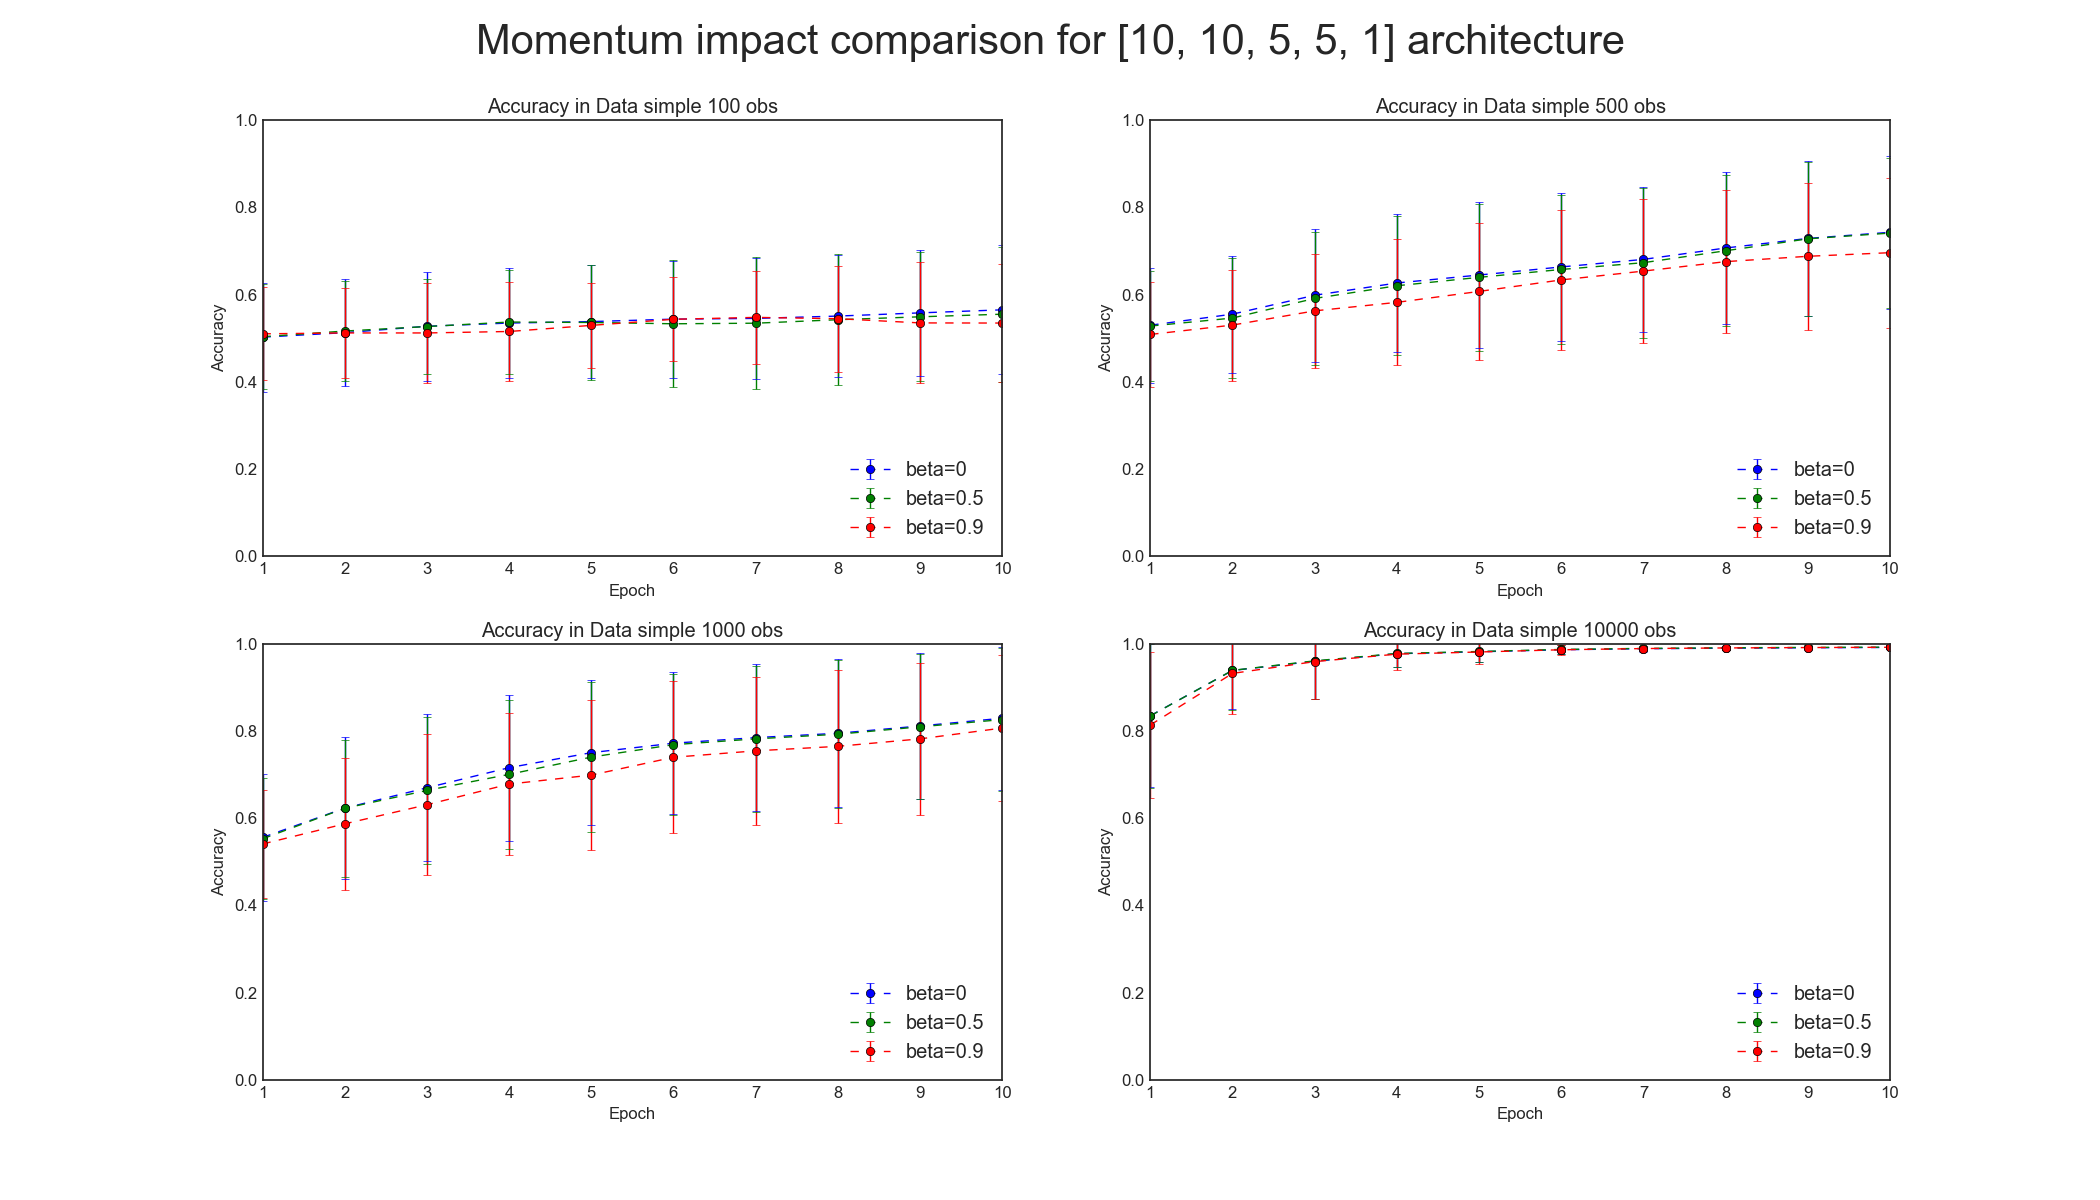
\includegraphics[width=1.4\textwidth]{results/classification/architecture-6/inertia_data_simple_2020_03_24_03_17_19.png}}
   \caption{Mean accuracy achieved on the test set.}
\end{figure}


\centerline{
\begin{tabular}{llll}
\hline
{} &        beta=0 &      beta=0.5 &      beta=0.9 \\
\hline
Data simple 100 obs   &  0.56 +- 0.15 &  0.55 +- 0.15 &  0.55 +- 0.11 \\
Data simple 500 obs   &  0.74 +- 0.18 &  0.74 +- 0.17 &  0.70 +- 0.17 \\
Data simple 1000 obs  &  0.83 +- 0.16 &  0.83 +- 0.16 &  0.81 +- 0.17 \\
Data simple 10000 obs &  0.99 +- 0.00 &  0.99 +- 0.00 &  0.99 +- 0.00 \\
\hline
\end{tabular}
}

\newpage
% ----------------- BS ACTIVATION DATA  -------------------------
\begin{figure}[!ht]
    \noindent\makebox[\textwidth]{%
   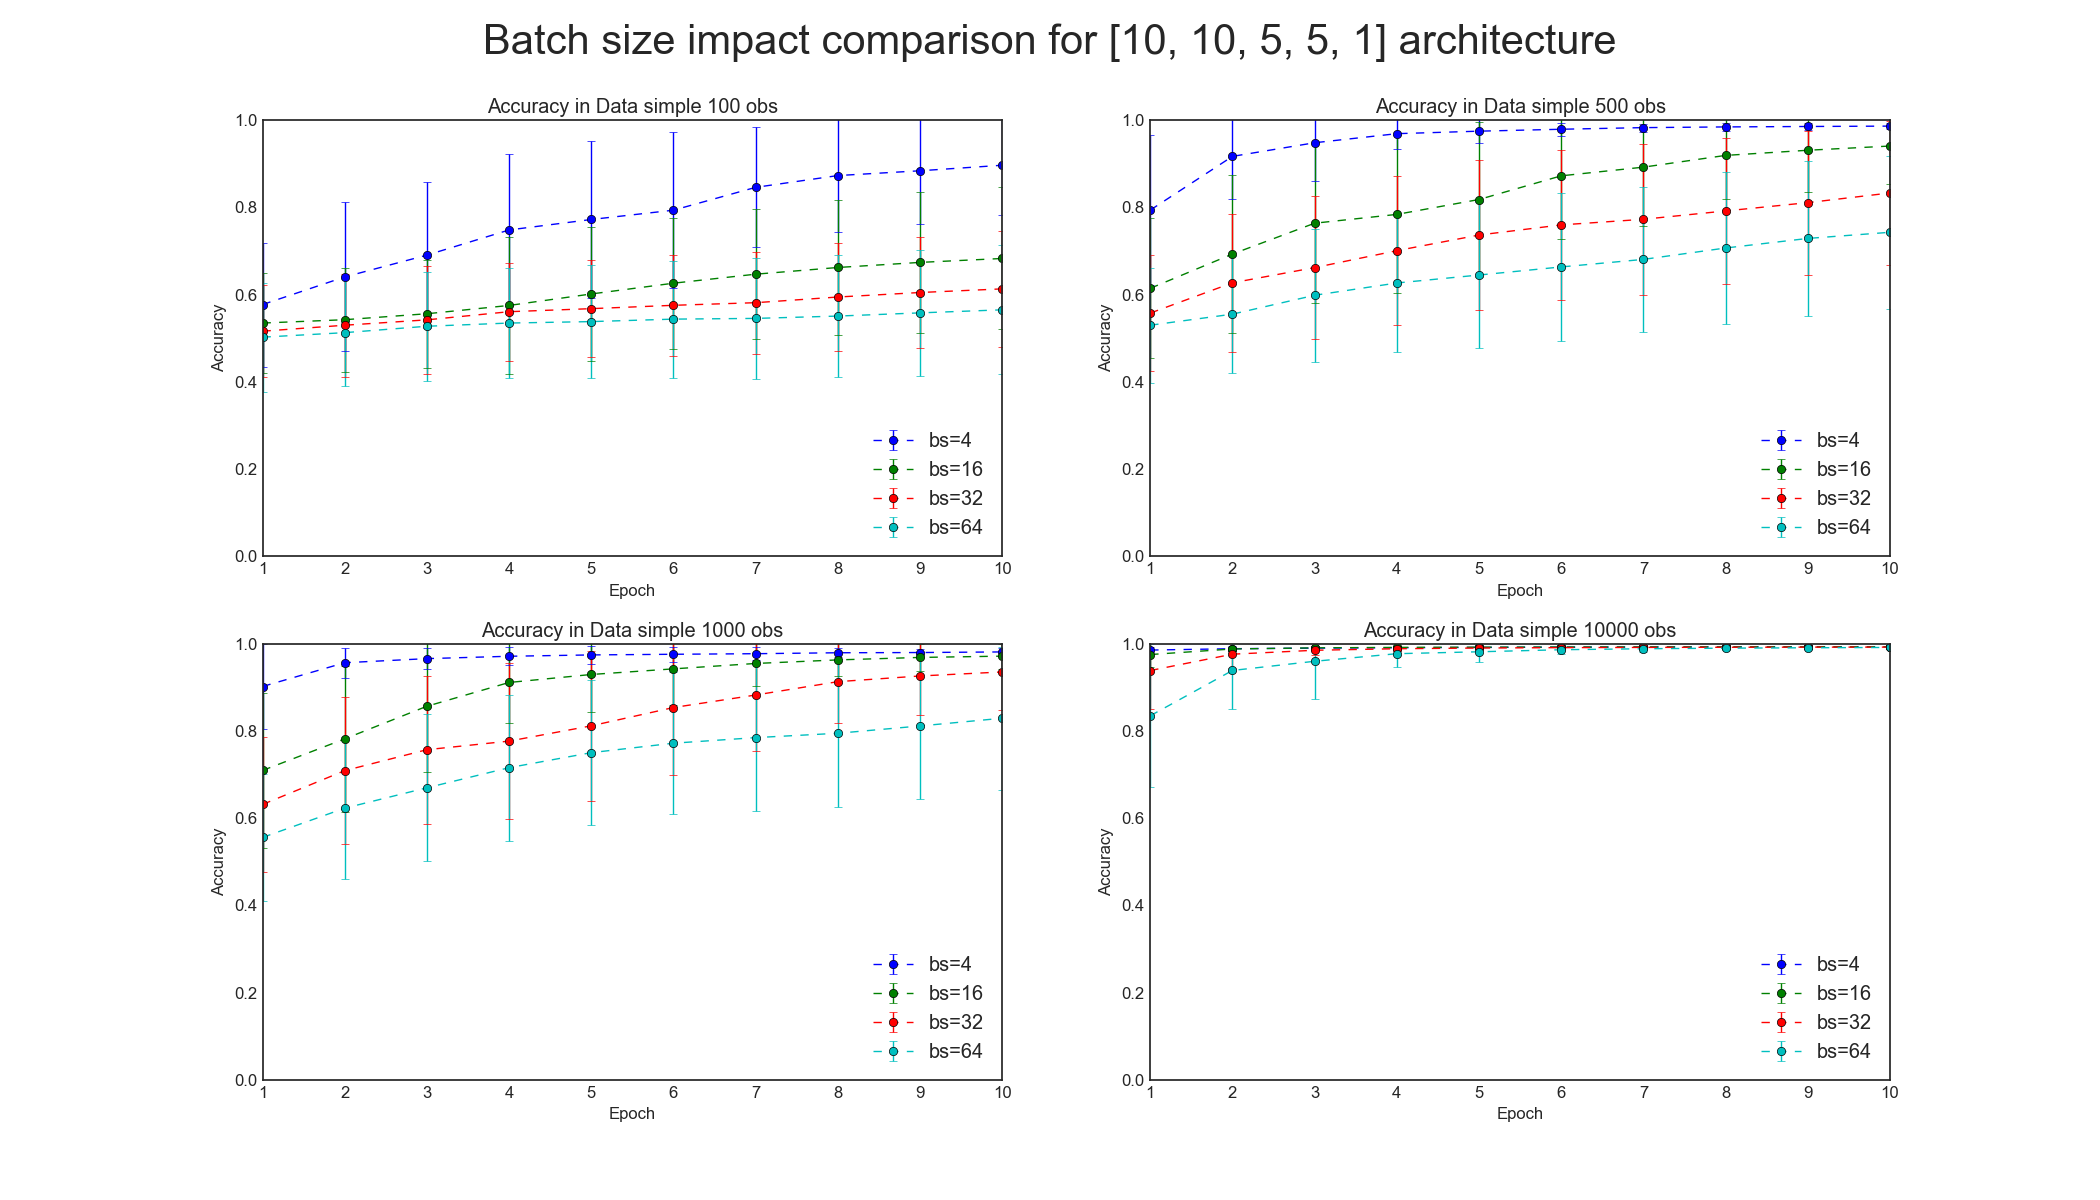
\includegraphics[width=1.4\textwidth]{results/classification/architecture-6/batch_size_data_simple_2020_03_24_03_17_20.png}}
   \caption{Mean accuracy achieved on the test set.}
\end{figure}

\centerline{
\begin{tabular}{lllll}
\hline
{} &          bs=4 &         bs=16 &         bs=32 &         bs=64 \\
\hline
Data simple 100 obs   &  0.90 +- 0.11 &  0.68 +- 0.16 &  0.61 +- 0.13 &  0.56 +- 0.15 \\
Data simple 500 obs   &  0.99 +- 0.01 &  0.94 +- 0.09 &  0.83 +- 0.17 &  0.74 +- 0.18 \\
Data simple 1000 obs  &  0.98 +- 0.01 &  0.97 +- 0.03 &  0.94 +- 0.09 &  0.83 +- 0.16 \\
Data simple 10000 obs &  0.99 +- 0.00 &  0.99 +- 0.00 &  0.99 +- 0.00 &  0.99 +- 0.00 \\
\hline
\end{tabular}
}


\newpage
\subsubsection{Conclusion}
Network converged on every tested combination of architecture and tested parameters. Impact of parameters on neural network performance was quite similar in every architecture: small learning rate made learning faster (we didn't have problems with exploding gradient), \texttt{leaky relu} and \texttt{tanh} were in most cases the best choice of activation functions, momentum value $\beta$ had really small impact on learning performance and small batch size made network converge faster. 

\newpage
\subsection{Three Gauss}
\subsubsection{Architecture 1}
\[[]\]
No hidden layers. 


% ----------------- LR ACTIVATION DATA  -------------------------

\begin{figure}[!ht]
    \noindent\makebox[\textwidth]{%
   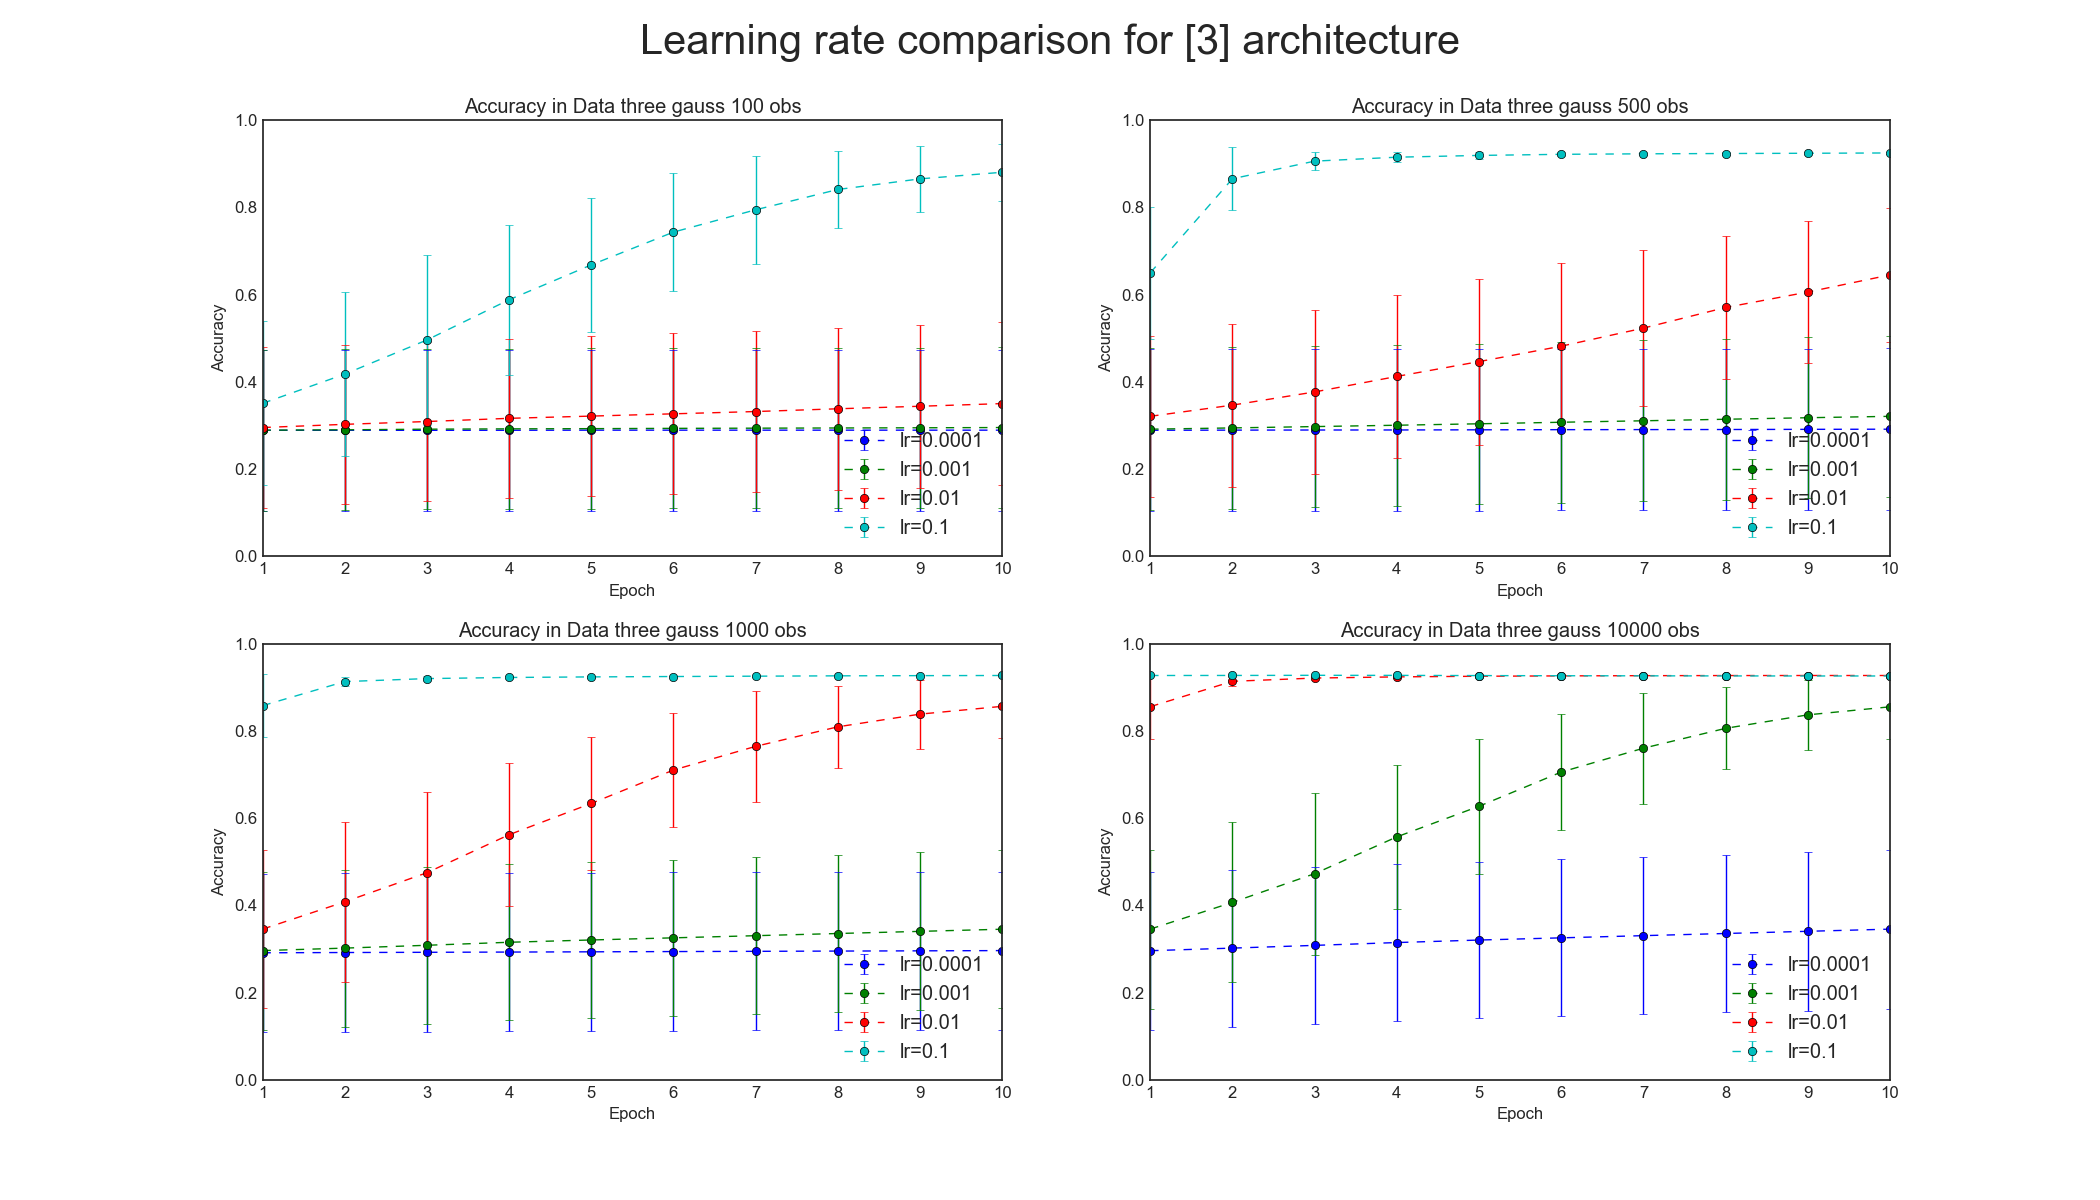
\includegraphics[width=1.4\textwidth]{results/classification/architecture-1/lr_data_gauss_2020_03_24_08_20_21.png}}
   \caption{Mean accuracy achieved on the test set.}
\end{figure}

\centerline{
\begin{tabular}{lllll}
\hline
{} &     lr=0.0001 &      lr=0.001 &       lr=0.01 &        lr=0.1 \\
\hline
Data three gauss 100 obs   &  0.29 +- 0.18 &  0.30 +- 0.18 &  0.35 +- 0.19 &  0.88 +- 0.07 \\
Data three gauss 500 obs   &  0.29 +- 0.18 &  0.32 +- 0.18 &  0.64 +- 0.15 &  0.92 +- 0.00 \\
Data three gauss 1000 obs  &  0.30 +- 0.18 &  0.35 +- 0.18 &  0.86 +- 0.07 &  0.93 +- 0.00 \\
Data three gauss 10000 obs &  0.35 +- 0.18 &  0.86 +- 0.07 &  0.93 +- 0.00 &  0.93 +- 0.00 \\
\hline
\end{tabular}
}

\newpage
% ----------------- AF ACTIVATION DATA  -------------------------
\begin{figure}[!ht]
    \noindent\makebox[\textwidth]{%
   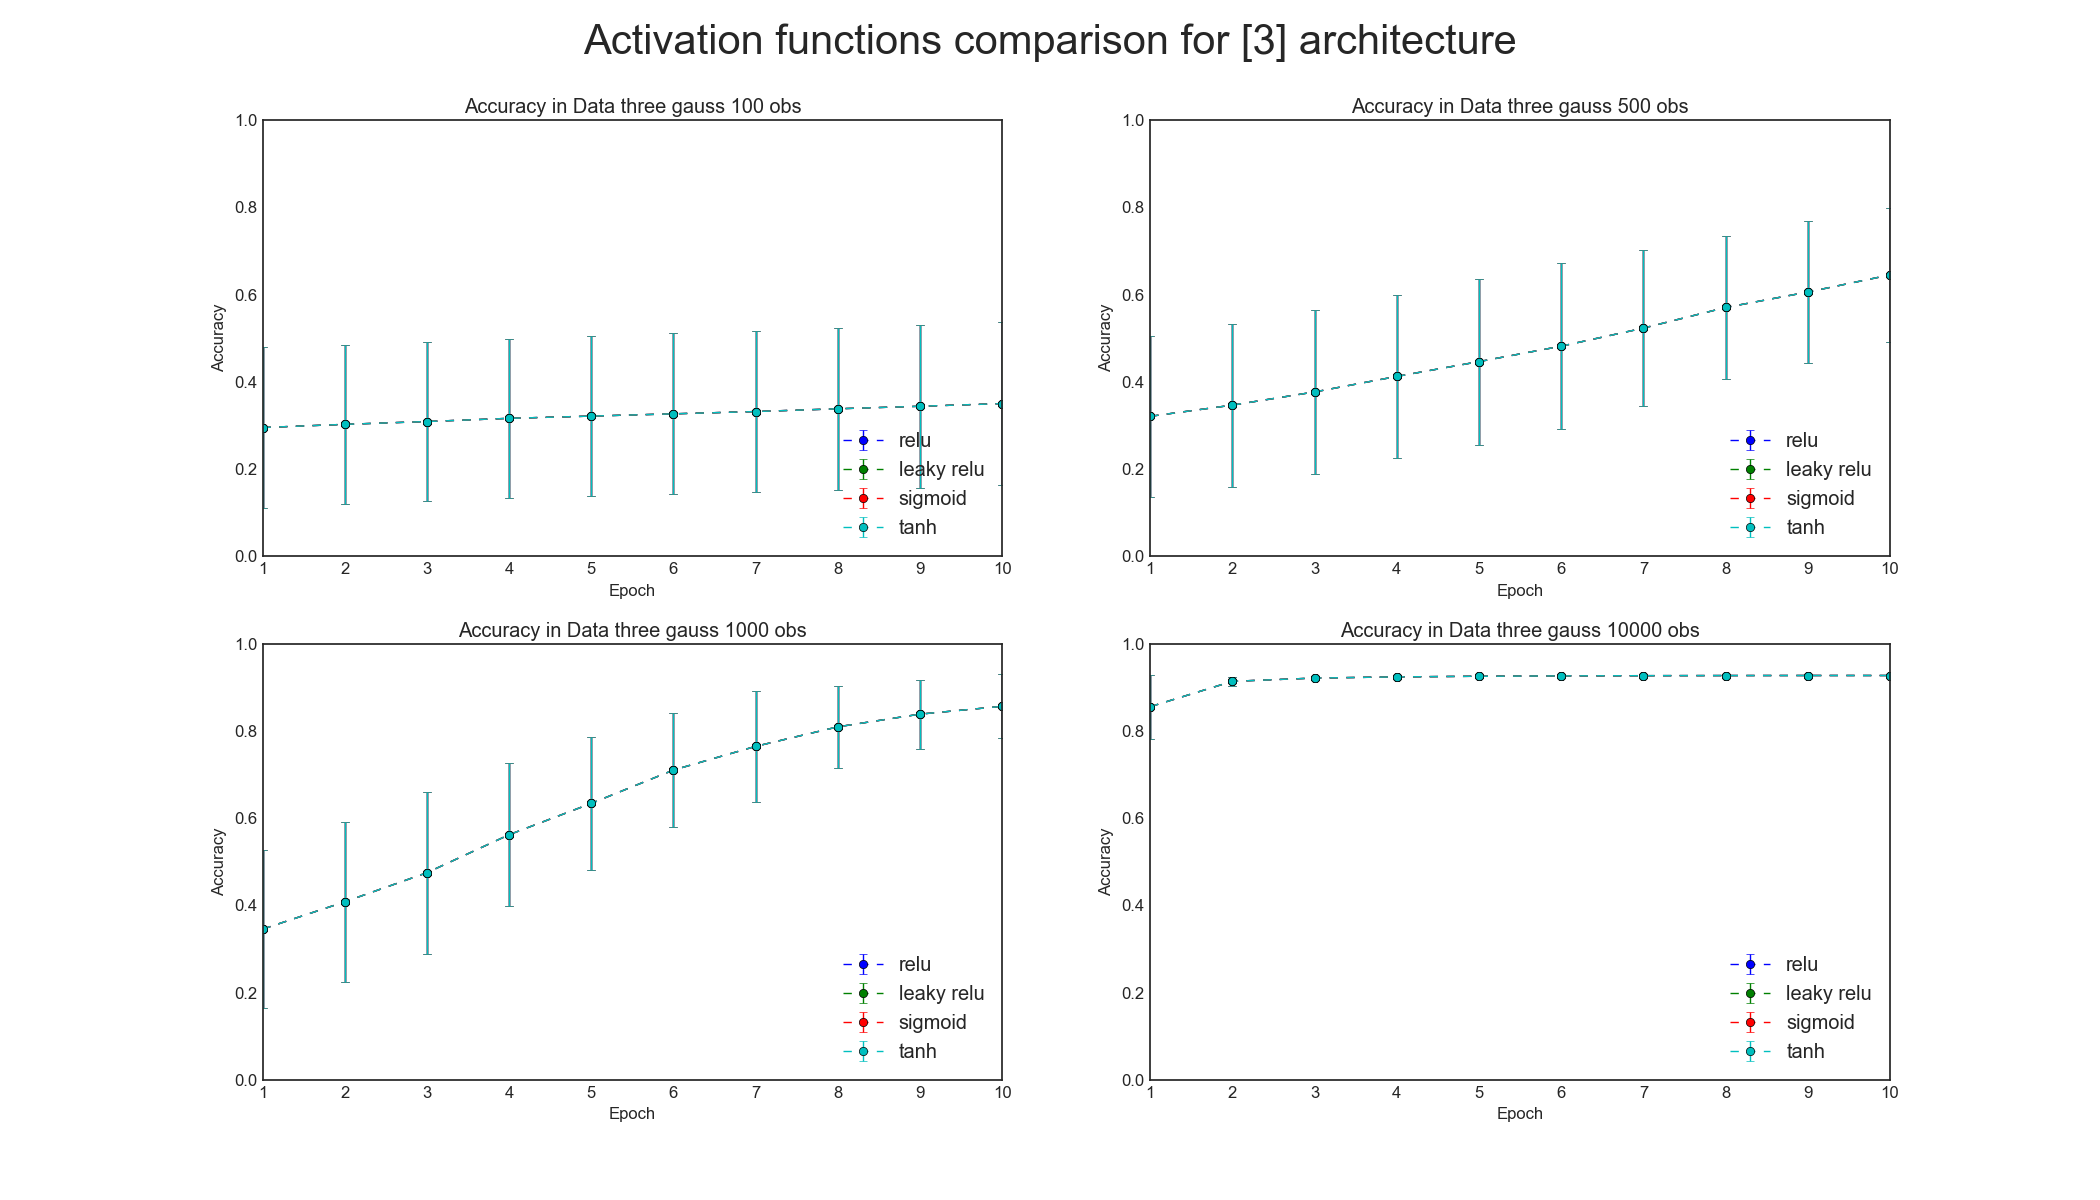
\includegraphics[width=1.4\textwidth]{results/classification/architecture-1/activation_function_data_gauss_2020_03_24_08_20_21.png}}
   \caption{Mean accuracy achieved on the test set.}
\end{figure}


\centerline{
\begin{tabular}{lllll}
\hline
{} &          relu &    leaky relu &       sigmoid &          tanh \\
\hline
Data three gauss 100 obs   &  0.35 +- 0.19 &  0.35 +- 0.19 &  0.35 +- 0.19 &  0.35 +- 0.19 \\
Data three gauss 500 obs   &  0.64 +- 0.15 &  0.64 +- 0.15 &  0.64 +- 0.15 &  0.64 +- 0.15 \\
Data three gauss 1000 obs  &  0.86 +- 0.07 &  0.86 +- 0.07 &  0.86 +- 0.07 &  0.86 +- 0.07 \\
Data three gauss 10000 obs &  0.93 +- 0.00 &  0.93 +- 0.00 &  0.93 +- 0.00 &  0.93 +- 0.00 \\
\hline
\end{tabular}
}

\newpage
% ----------------- INERTIA ACTIVATION DATA  -------------------------
\begin{figure}[!ht]
    \noindent\makebox[\textwidth]{%
   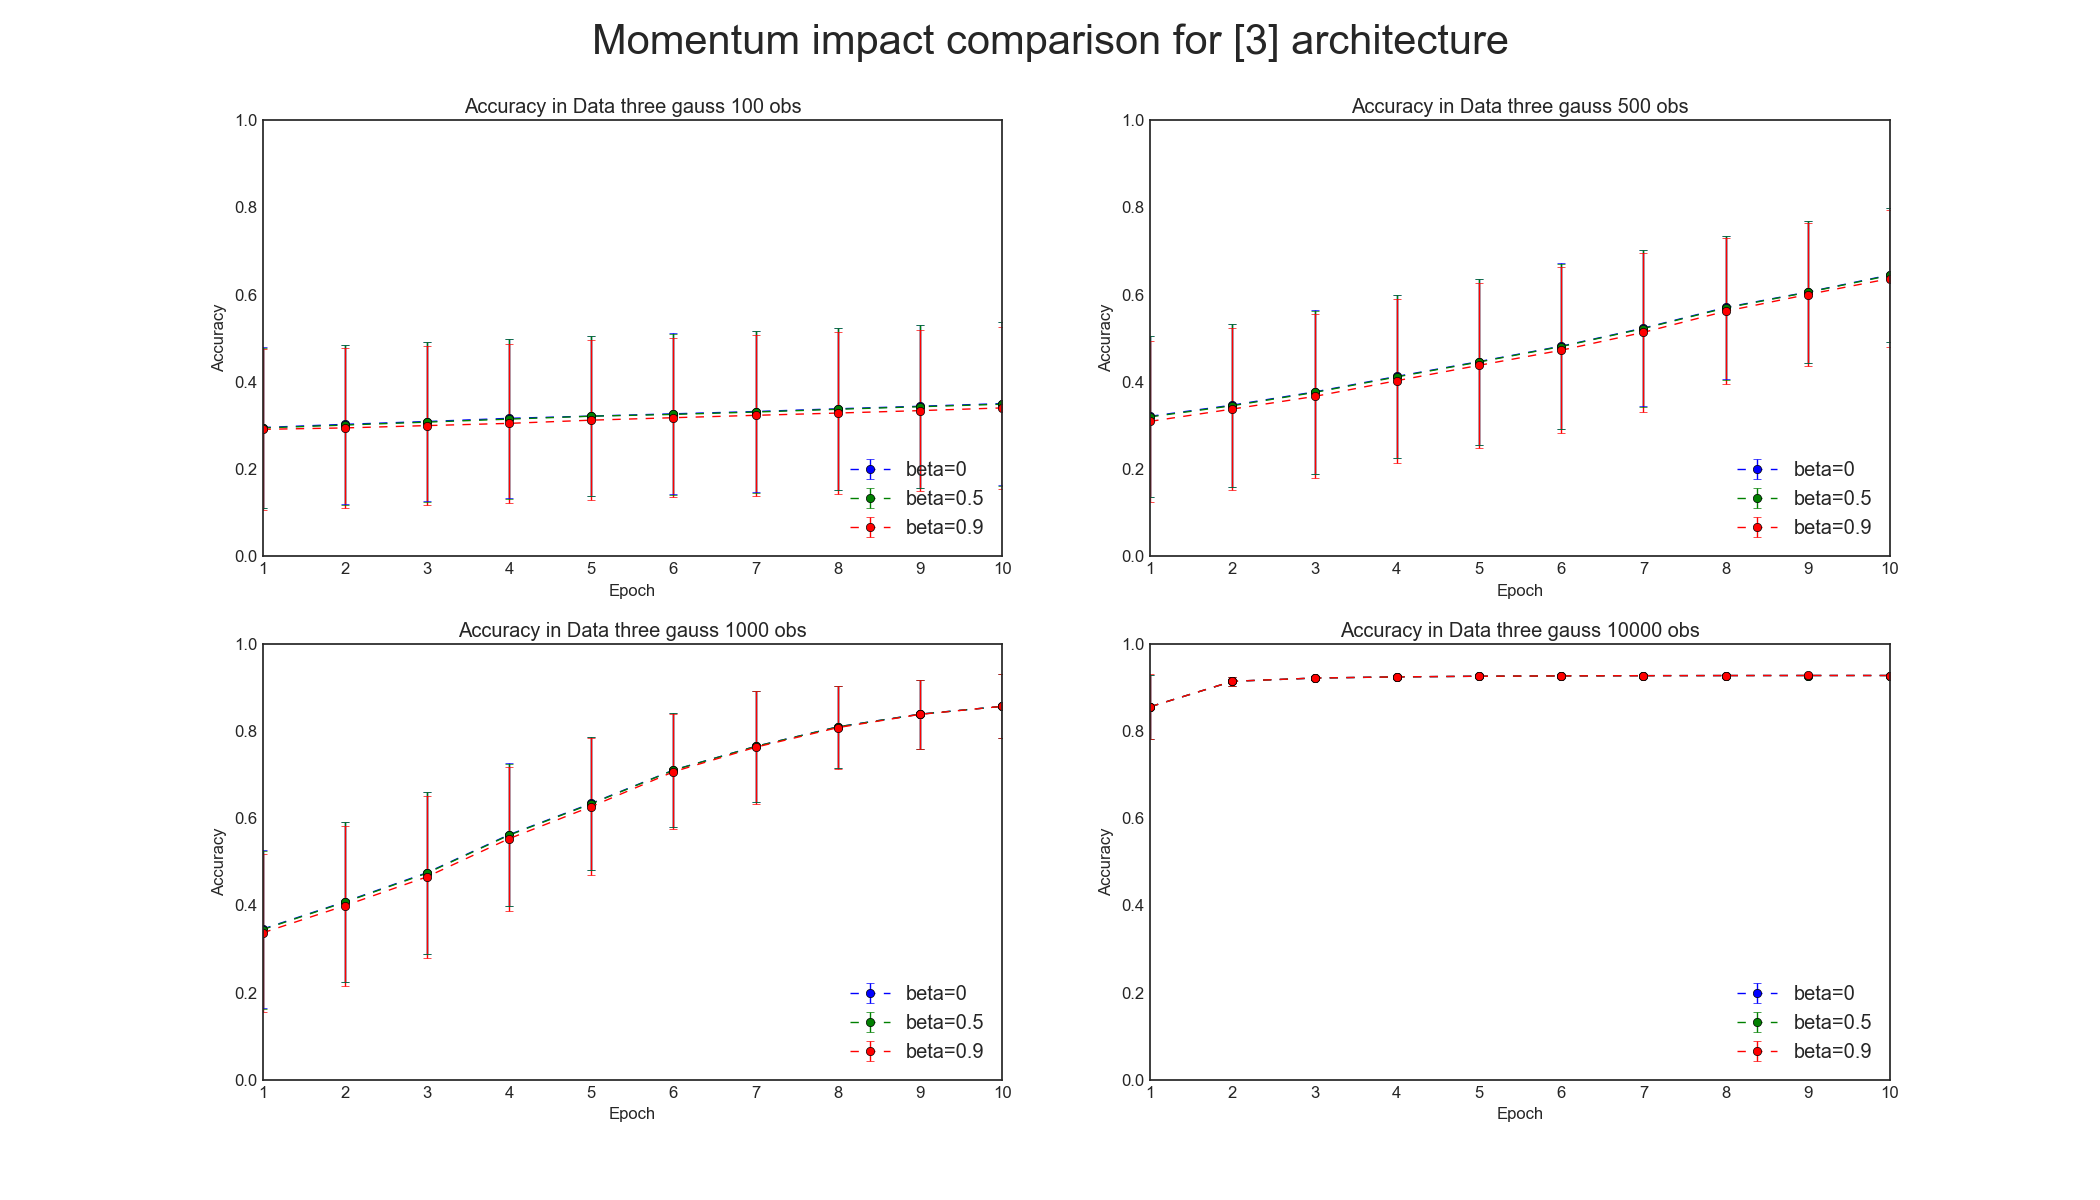
\includegraphics[width=1.4\textwidth]{results/classification/architecture-1/inertia_data_gauss_2020_03_24_08_20_22.png}}
   \caption{Mean accuracy achieved on the test set.}
\end{figure}


\centerline{
\begin{tabular}{llll}
\hline
{} &        beta=0 &      beta=0.5 &      beta=0.9 \\
\hline
Data three gauss 100 obs   &  0.35 +- 0.19 &  0.35 +- 0.19 &  0.34 +- 0.19 \\
Data three gauss 500 obs   &  0.64 +- 0.15 &  0.64 +- 0.15 &  0.64 +- 0.16 \\
Data three gauss 1000 obs  &  0.86 +- 0.07 &  0.86 +- 0.07 &  0.86 +- 0.07 \\
Data three gauss 10000 obs &  0.93 +- 0.00 &  0.93 +- 0.00 &  0.93 +- 0.00 \\
\hline
\end{tabular}
}

\newpage
% ----------------- BS ACTIVATION DATA  -------------------------
\begin{figure}[!ht]
    \noindent\makebox[\textwidth]{%
   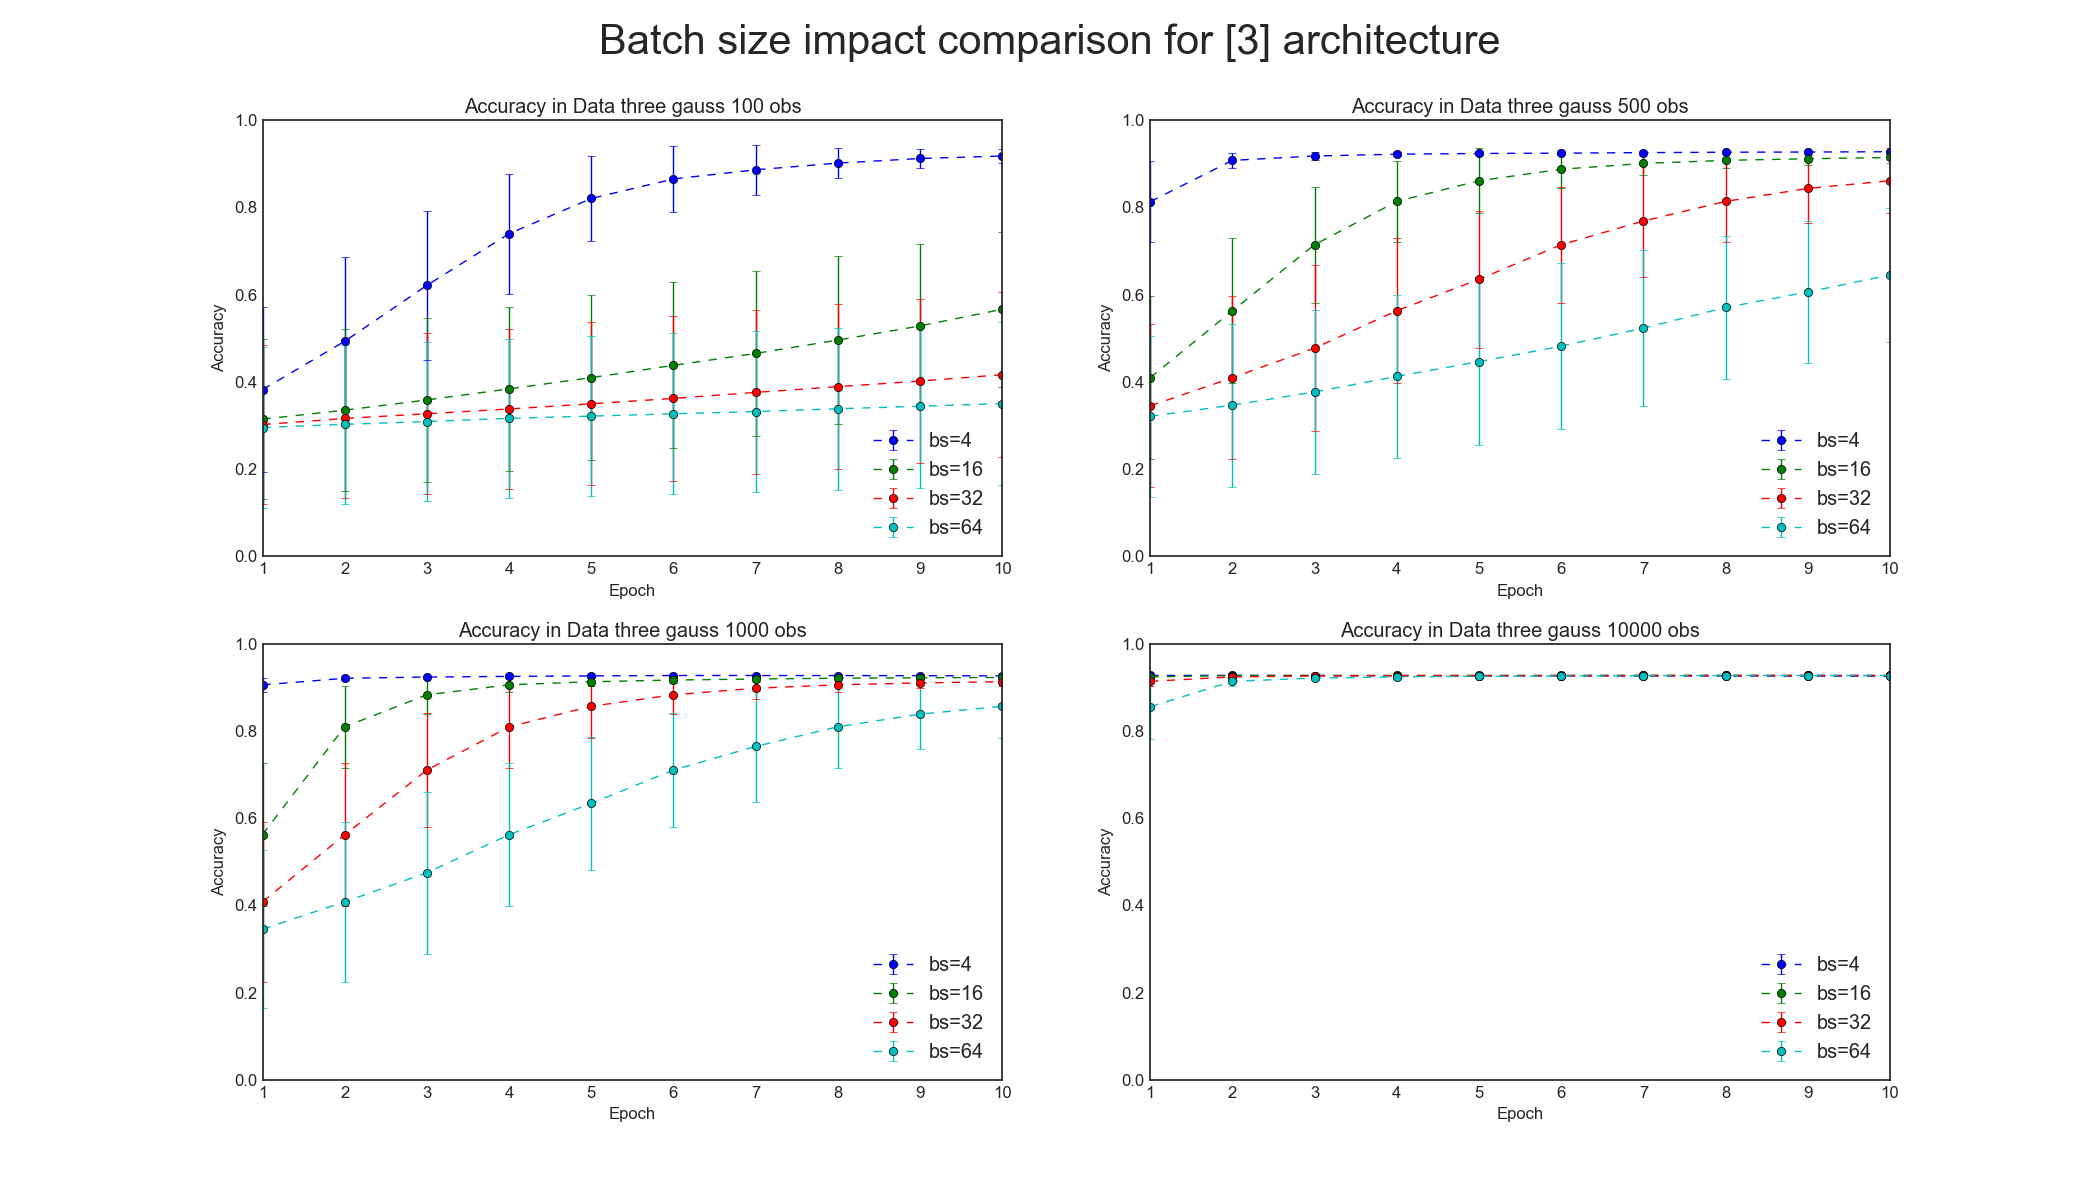
\includegraphics[width=1.4\textwidth]{results/classification/architecture-1/batch_size_data_gauss_2020_03_24_08_20_22.png}}
   \caption{Mean accuracy achieved on the test set.}
\end{figure}

\centerline{
\begin{tabular}{lllll}
\hline
{} &          bs=4 &         bs=16 &         bs=32 &         bs=64 \\
\hline
Data three gauss 100 obs   &  0.92 +- 0.02 &  0.57 +- 0.18 &  0.42 +- 0.19 &  0.35 +- 0.19 \\
Data three gauss 500 obs   &  0.93 +- 0.00 &  0.91 +- 0.01 &  0.86 +- 0.07 &  0.64 +- 0.15 \\
Data three gauss 1000 obs  &  0.93 +- 0.00 &  0.92 +- 0.00 &  0.91 +- 0.01 &  0.86 +- 0.07 \\
Data three gauss 10000 obs &  0.93 +- 0.00 &  0.93 +- 0.00 &  0.93 +- 0.00 &  0.93 +- 0.00 \\
\hline
\end{tabular}
}



\newpage
\subsubsection{Architecture 2}
\[[5]\]
One hidden layer with 5 neurons.

% ----------------- LR ACTIVATION DATA  -------------------------

\begin{figure}[!ht]
    \noindent\makebox[\textwidth]{%
   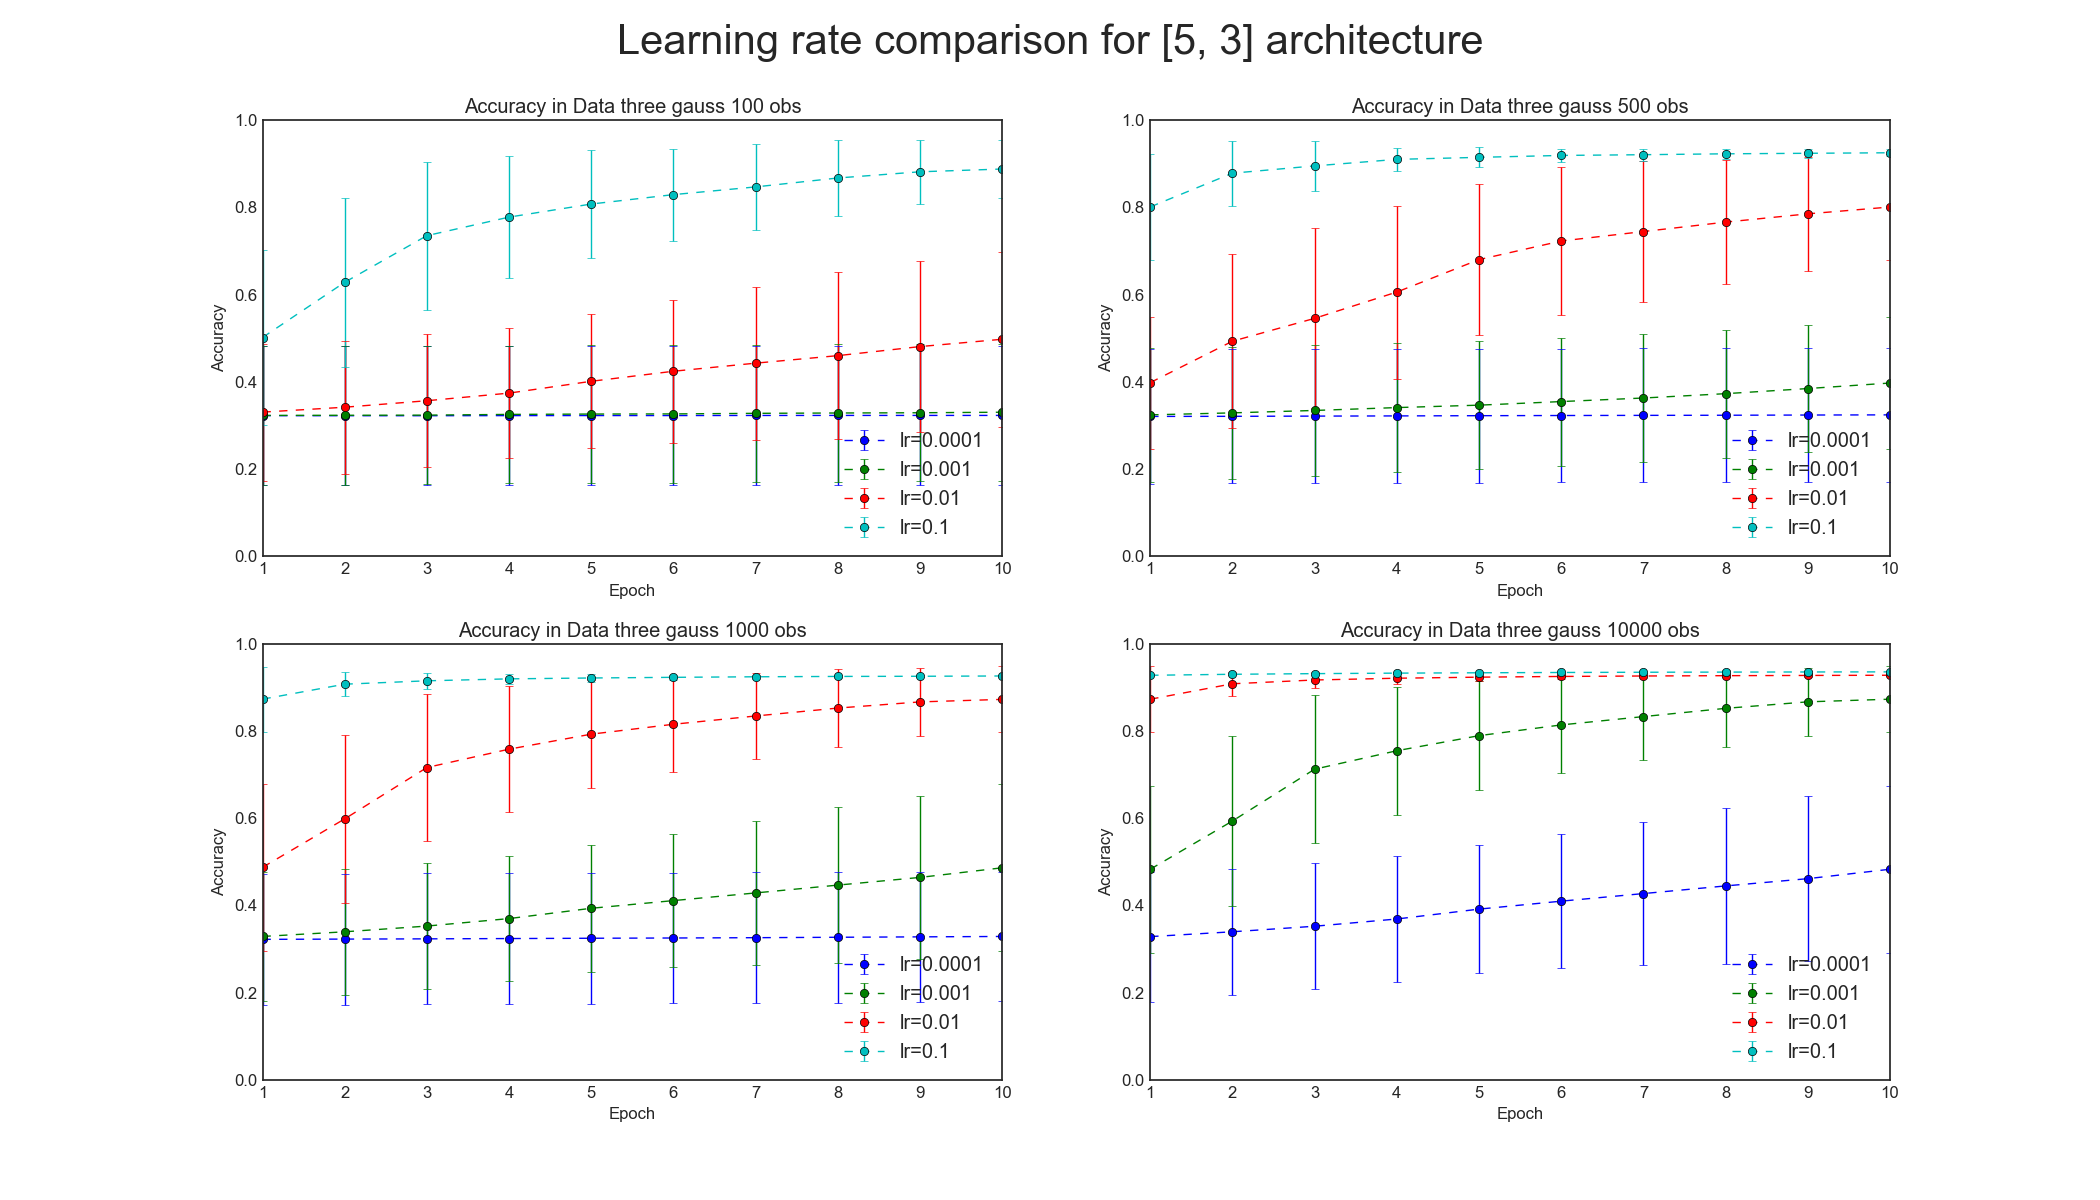
\includegraphics[width=1.4\textwidth]{results/classification/architecture-2/lr_data_gauss_2020_03_24_08_51_54.png}}
   \caption{Mean accuracy achieved on the test set.}
\end{figure}

\centerline{
\begin{tabular}{lllll}
\hline
{} &     lr=0.0001 &      lr=0.001 &       lr=0.01 &        lr=0.1 \\
\hline
Data three gauss 100 obs   &  0.32 +- 0.16 &  0.33 +- 0.16 &  0.50 +- 0.20 &  0.89 +- 0.07 \\
Data three gauss 500 obs   &  0.32 +- 0.15 &  0.40 +- 0.15 &  0.80 +- 0.12 &  0.92 +- 0.01 \\
Data three gauss 1000 obs  &  0.33 +- 0.15 &  0.49 +- 0.19 &  0.87 +- 0.08 &  0.93 +- 0.00 \\
Data three gauss 10000 obs &  0.48 +- 0.19 &  0.87 +- 0.08 &  0.93 +- 0.00 &  0.94 +- 0.00 \\
\hline
\end{tabular}
}

\newpage
% ----------------- AF ACTIVATION DATA  -------------------------
\begin{figure}[!ht]
    \noindent\makebox[\textwidth]{%
   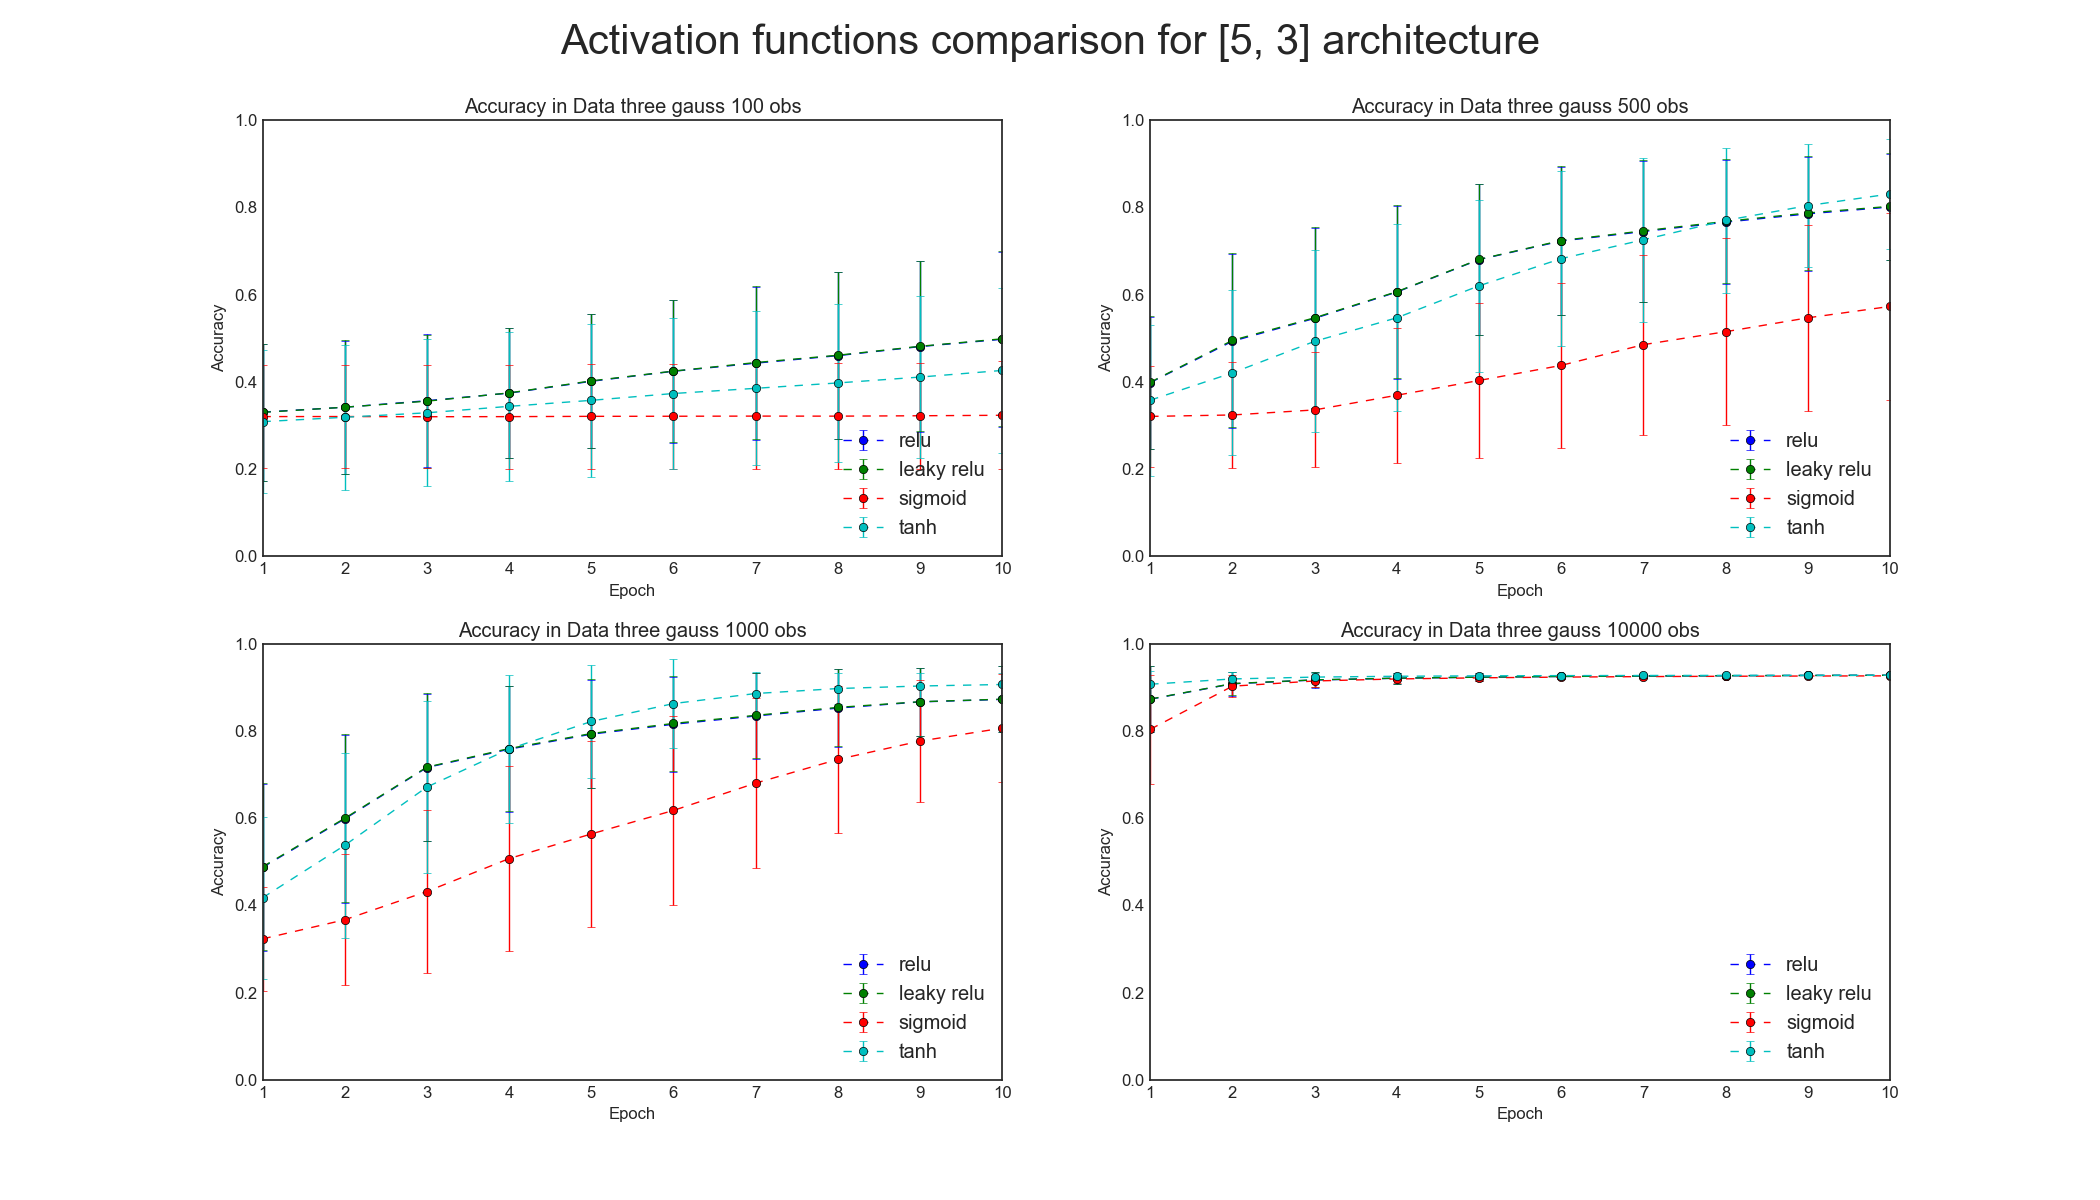
\includegraphics[width=1.4\textwidth]{results/classification/architecture-2/activation_function_data_gauss_2020_03_24_08_51_54.png}}
   \caption{Mean accuracy achieved on the test set.}
\end{figure}


\centerline{
\begin{tabular}{lllll}
\hline
{} &          relu &    leaky relu &       sigmoid &          tanh \\
\hline
Data three gauss 100 obs   &  0.50 +- 0.20 &  0.50 +- 0.20 &  0.32 +- 0.12 &  0.43 +- 0.19 \\
Data three gauss 500 obs   &  0.80 +- 0.12 &  0.80 +- 0.12 &  0.57 +- 0.21 &  0.83 +- 0.13 \\
Data three gauss 1000 obs  &  0.87 +- 0.08 &  0.87 +- 0.08 &  0.81 +- 0.12 &  0.91 +- 0.03 \\
Data three gauss 10000 obs &  0.93 +- 0.00 &  0.93 +- 0.00 &  0.93 +- 0.00 &  0.93 +- 0.00 \\
\hline
\end{tabular}
}

\newpage
% ----------------- INERTIA ACTIVATION DATA  -------------------------
\begin{figure}[!ht]
    \noindent\makebox[\textwidth]{%
   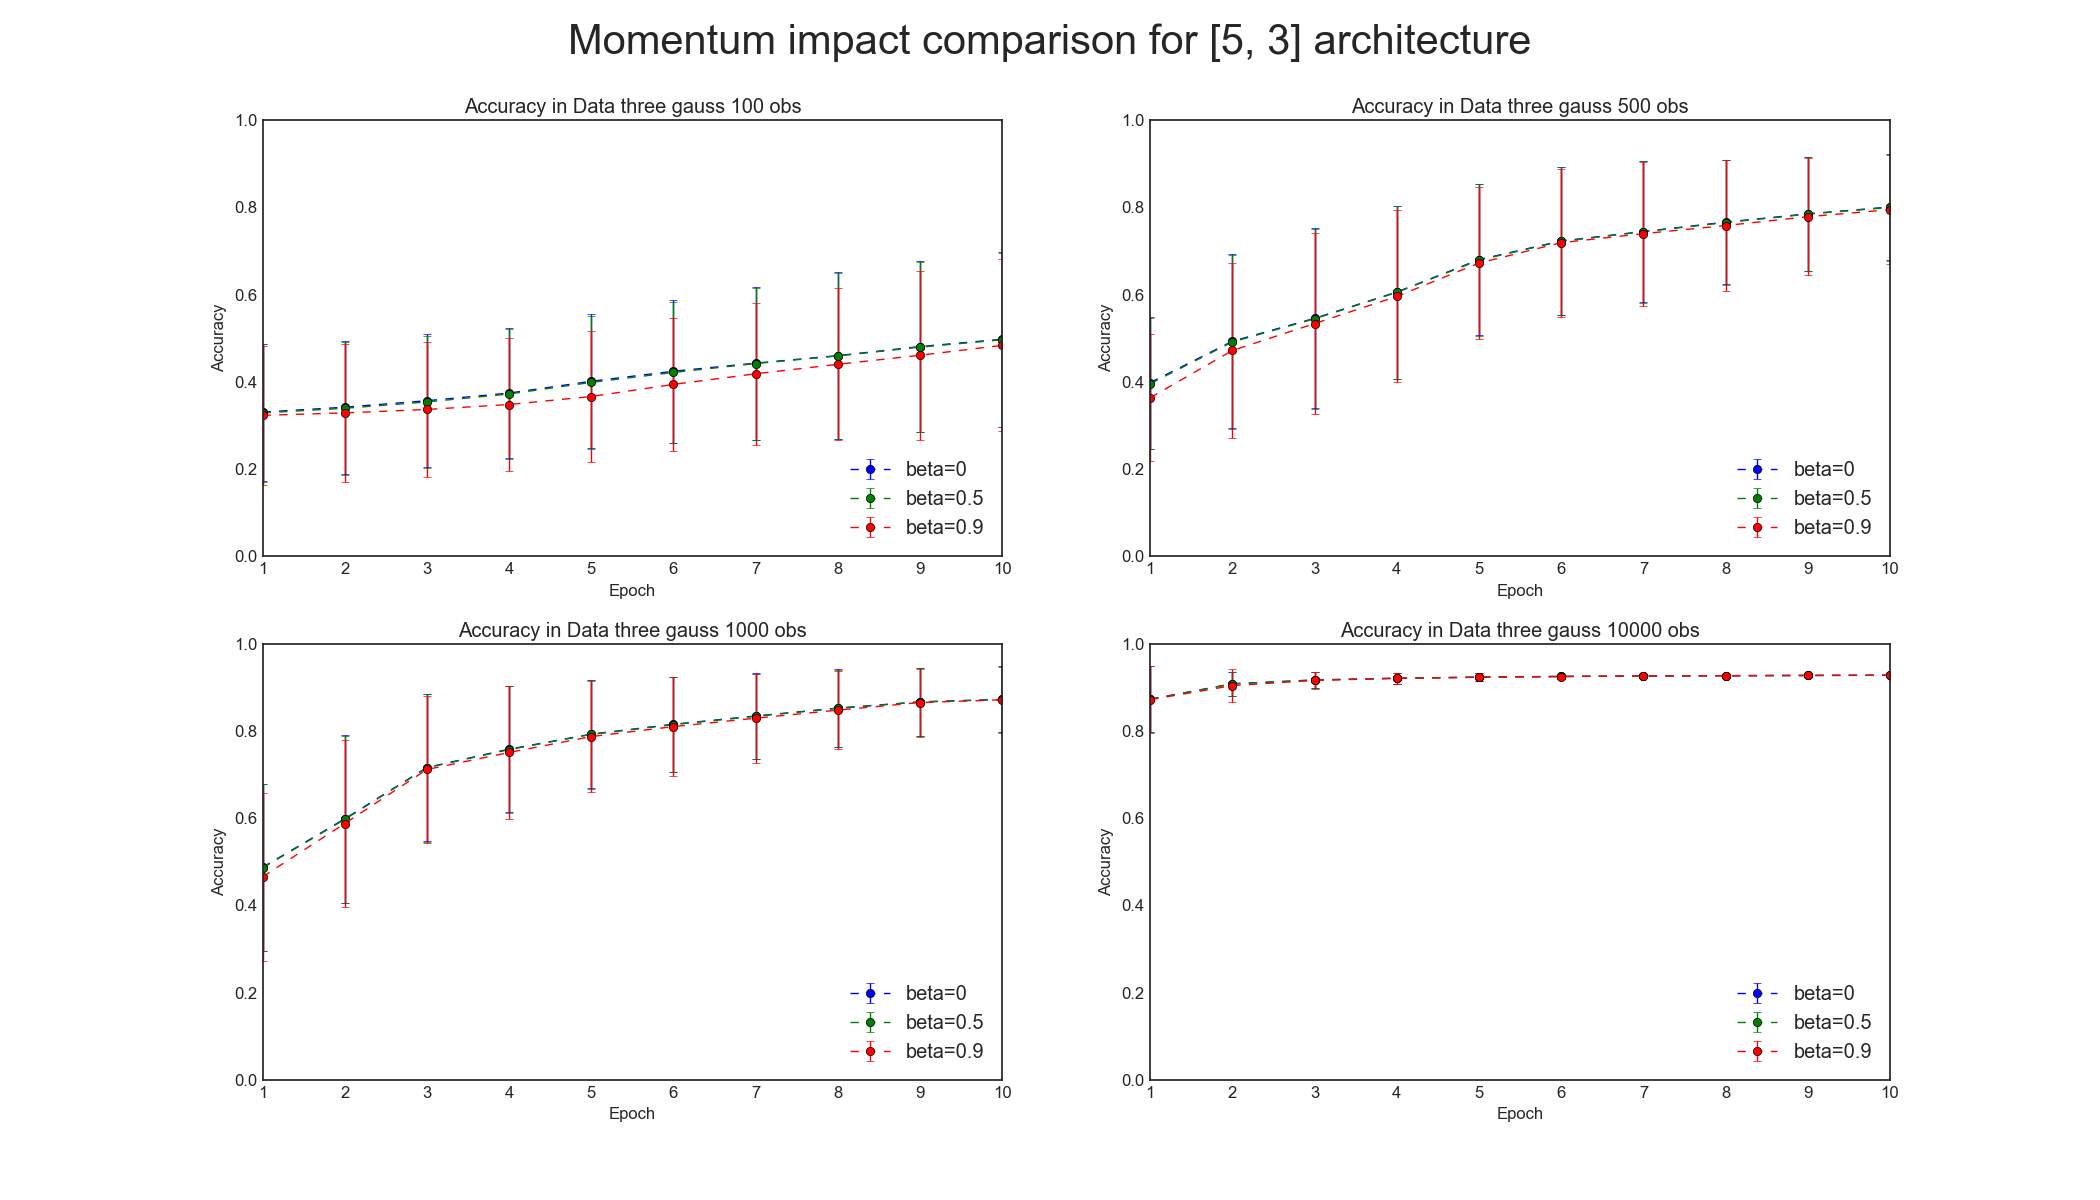
\includegraphics[width=1.4\textwidth]{results/classification/architecture-2/inertia_data_gauss_2020_03_24_08_51_54.png}}
   \caption{Mean accuracy achieved on the test set.}
\end{figure}


\centerline{
\begin{tabular}{llll}
\hline
{} &        beta=0 &      beta=0.5 &      beta=0.9 \\
\hline
Data three gauss 100 obs   &  0.50 +- 0.20 &  0.50 +- 0.20 &  0.48 +- 0.20 \\
Data three gauss 500 obs   &  0.80 +- 0.12 &  0.80 +- 0.12 &  0.79 +- 0.13 \\
Data three gauss 1000 obs  &  0.87 +- 0.08 &  0.87 +- 0.08 &  0.87 +- 0.08 \\
Data three gauss 10000 obs &  0.93 +- 0.00 &  0.93 +- 0.00 &  0.93 +- 0.00 \\
\hline
\end{tabular}
}

\newpage
% ----------------- BS ACTIVATION DATA  -------------------------
\begin{figure}[!ht]
    \noindent\makebox[\textwidth]{%
   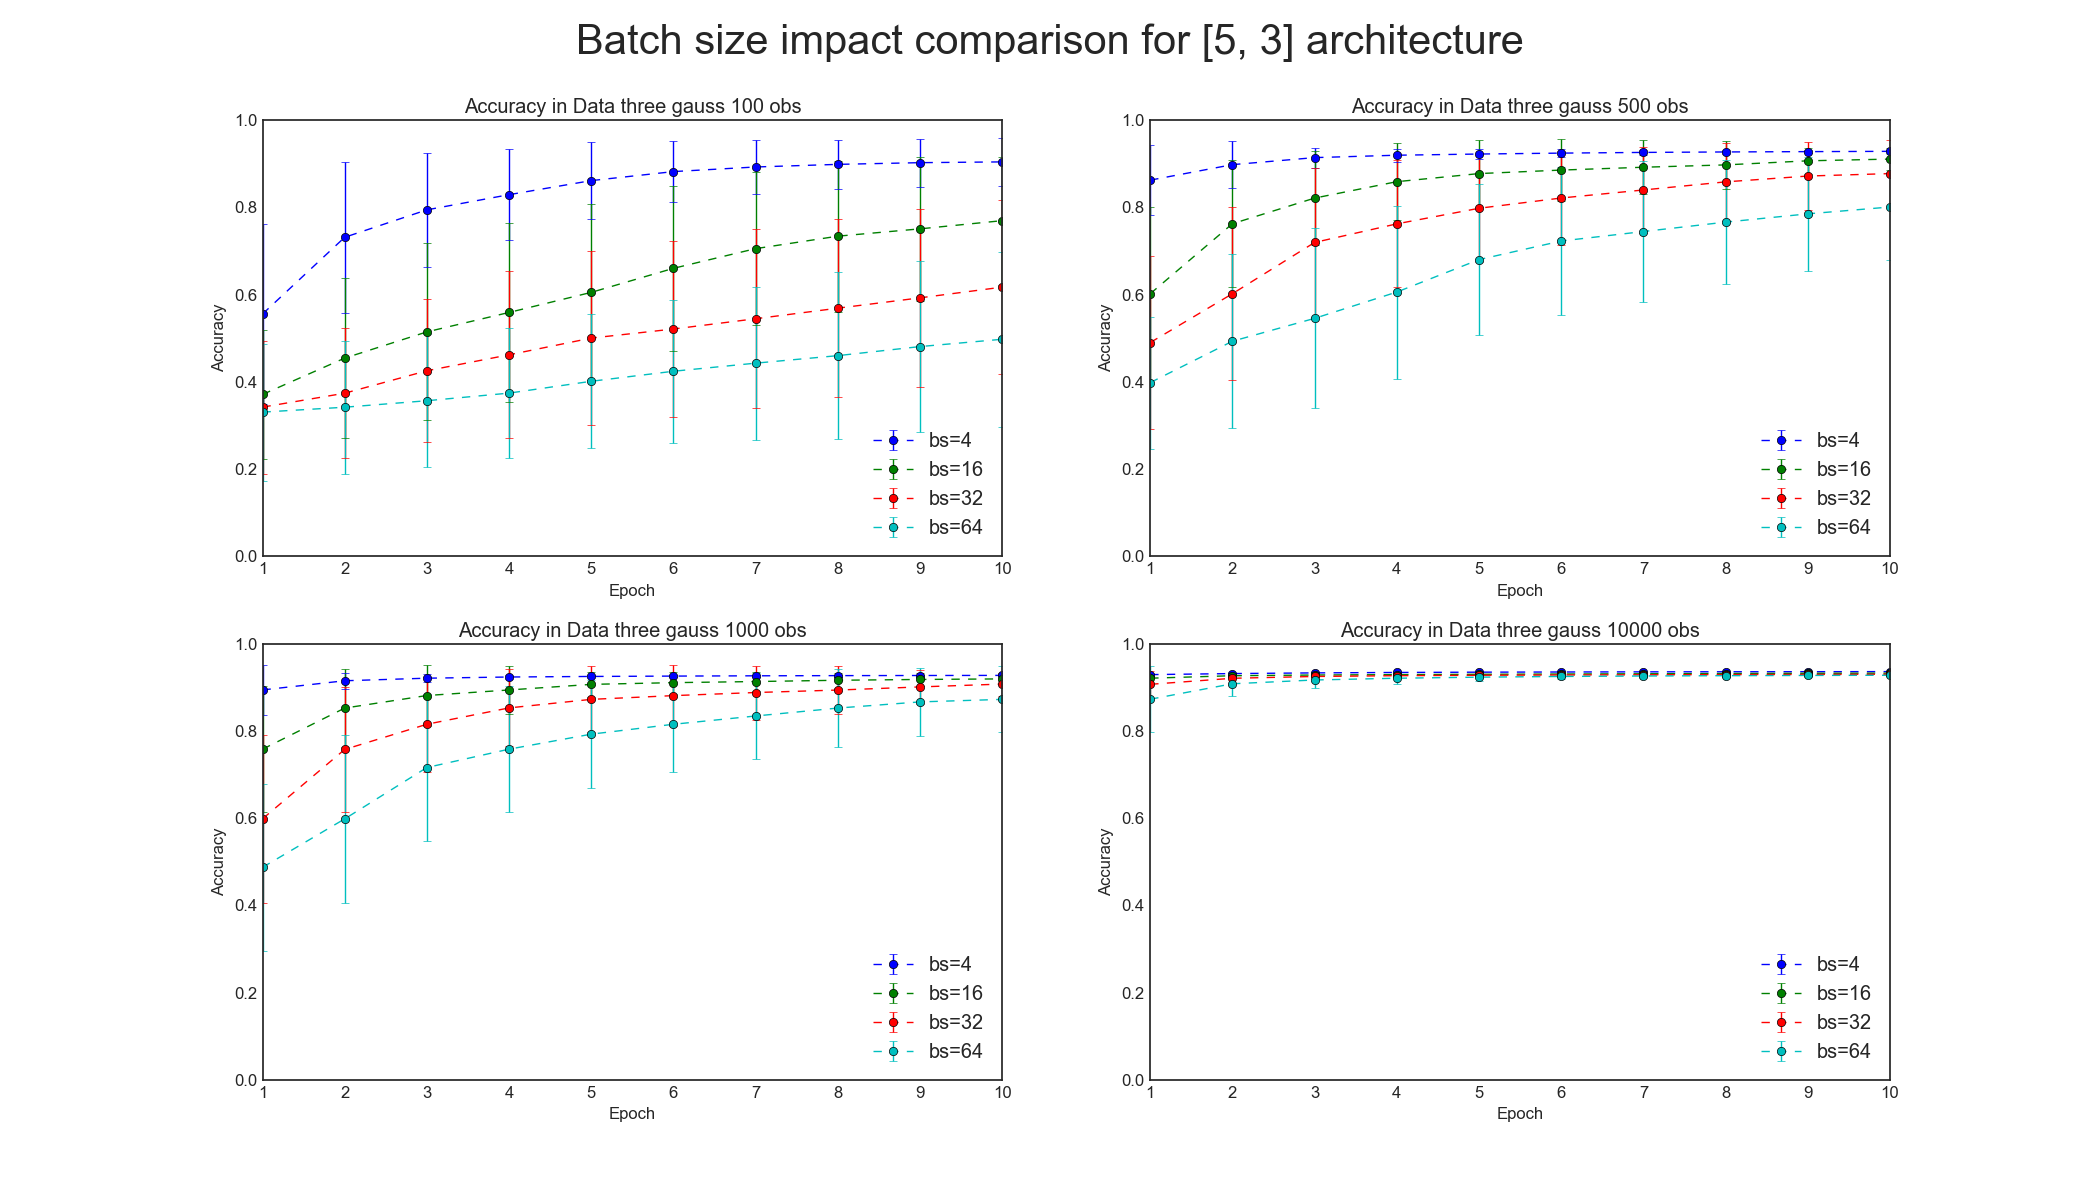
\includegraphics[width=1.4\textwidth]{results/classification/architecture-2/batch_size_data_gauss_2020_03_24_08_51_55.png}}
   \caption{Mean accuracy achieved on the test set.}
\end{figure}

\centerline{
\begin{tabular}{lllll}
\hline
{} &          bs=4 &         bs=16 &         bs=32 &         bs=64 \\
\hline
Data three gauss 100 obs   &  0.90 +- 0.05 &  0.77 +- 0.15 &  0.62 +- 0.20 &  0.50 +- 0.20 \\
Data three gauss 500 obs   &  0.93 +- 0.00 &  0.91 +- 0.03 &  0.88 +- 0.08 &  0.80 +- 0.12 \\
Data three gauss 1000 obs  &  0.93 +- 0.00 &  0.92 +- 0.01 &  0.91 +- 0.03 &  0.87 +- 0.08 \\
Data three gauss 10000 obs &  0.94 +- 0.00 &  0.93 +- 0.00 &  0.93 +- 0.00 &  0.93 +- 0.00 \\
\hline
\end{tabular}
}

\newpage
\subsubsection{Architecture 3}
\[[5, 5]\]
Two hidden layers, each with 5 neurons.

% ----------------- LR ACTIVATION DATA  -------------------------

\begin{figure}[!ht]
    \noindent\makebox[\textwidth]{%
   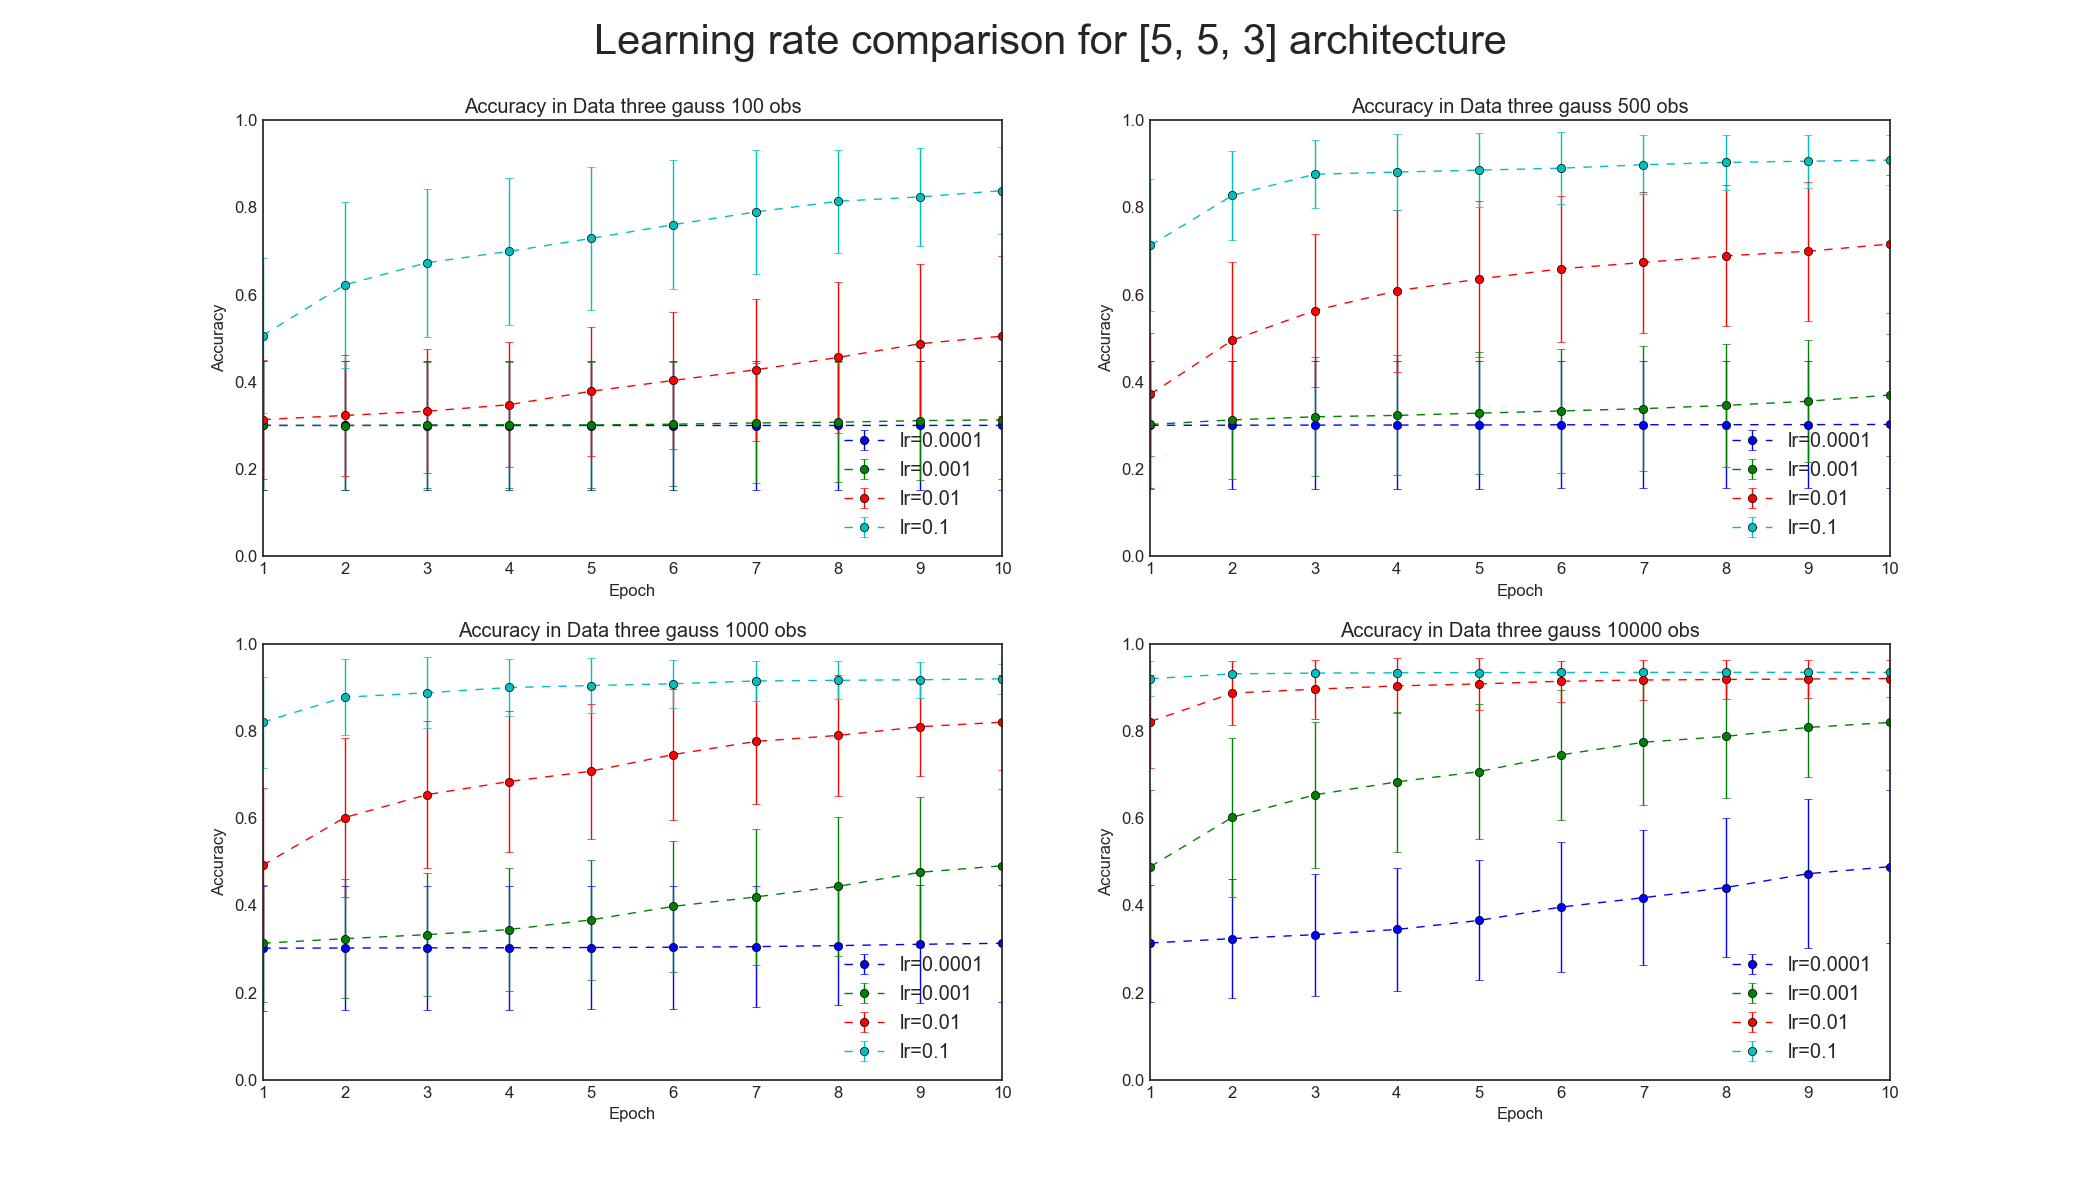
\includegraphics[width=1.4\textwidth]{results/classification/architecture-3/lr_data_gauss_2020_03_24_09_27_17.png}}
   \caption{Mean accuracy achieved on the test set.}
\end{figure}

\centerline{
\begin{tabular}{lllll}
\hline
{} &     lr=0.0001 &      lr=0.001 &       lr=0.01 &        lr=0.1 \\
\hline
Data three gauss 100 obs   &  0.30 +- 0.15 &  0.31 +- 0.14 &  0.50 +- 0.18 &  0.84 +- 0.10 \\
Data three gauss 500 obs   &  0.30 +- 0.14 &  0.37 +- 0.14 &  0.72 +- 0.16 &  0.91 +- 0.06 \\
Data three gauss 1000 obs  &  0.31 +- 0.13 &  0.49 +- 0.18 &  0.82 +- 0.11 &  0.92 +- 0.03 \\
Data three gauss 10000 obs &  0.49 +- 0.18 &  0.82 +- 0.11 &  0.92 +- 0.04 &  0.93 +- 0.00 \\
\hline
\end{tabular}
}

\newpage
% ----------------- AF ACTIVATION DATA  -------------------------
\begin{figure}[!ht]
    \noindent\makebox[\textwidth]{%
   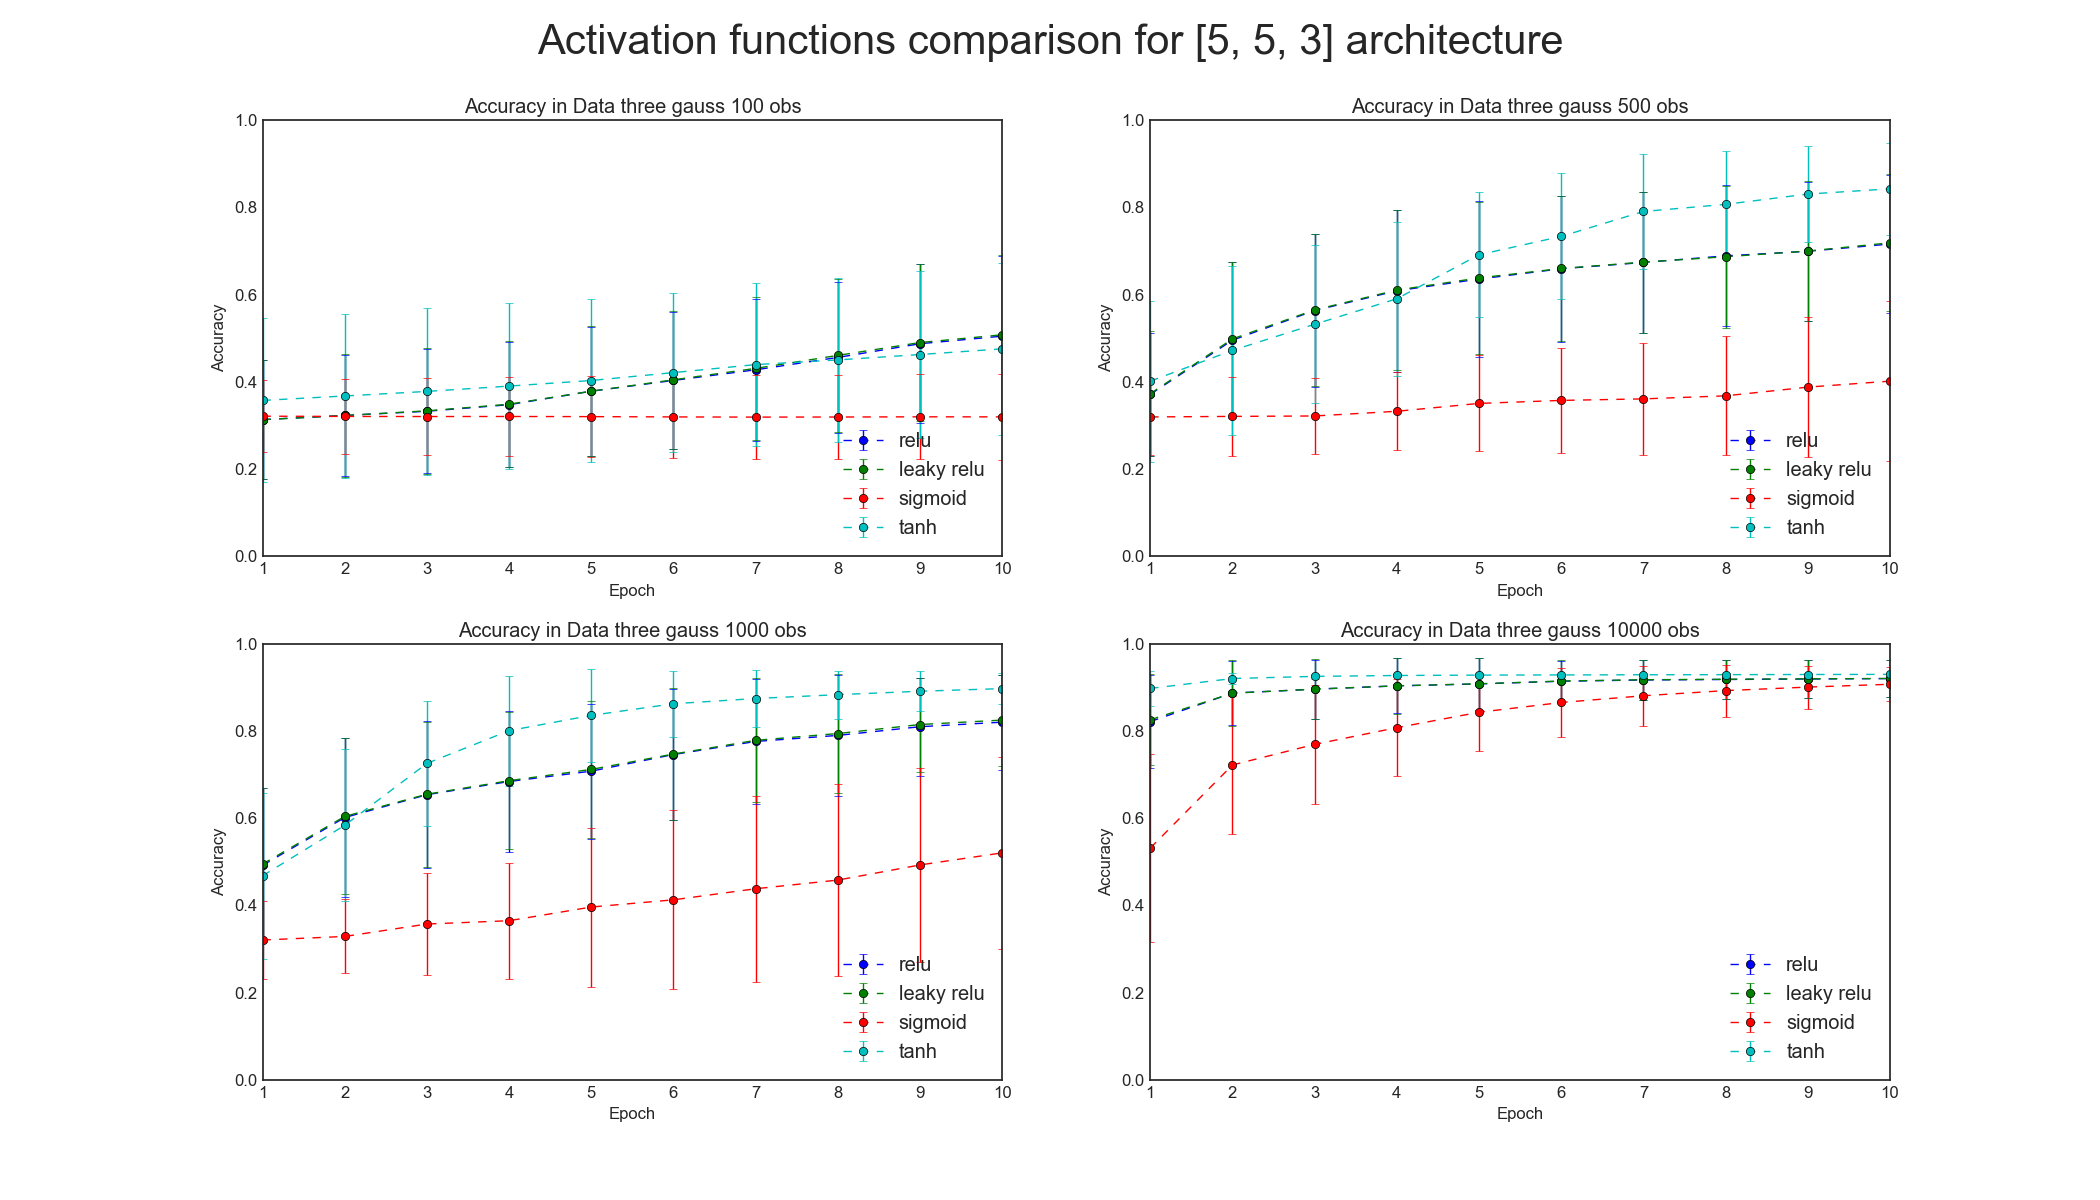
\includegraphics[width=1.4\textwidth]{results/classification/architecture-3/activation_function_data_gauss_2020_03_24_09_27_17.png}}
   \caption{Mean accuracy achieved on the test set.}
\end{figure}


\centerline{
\begin{tabular}{lllll}
\hline
{} &          relu &    leaky relu &       sigmoid &          tanh \\
\hline
Data three gauss 100 obs   &  0.50 +- 0.18 &  0.51 +- 0.18 &  0.32 +- 0.08 &  0.48 +- 0.20 \\
Data three gauss 500 obs   &  0.72 +- 0.16 &  0.72 +- 0.16 &  0.40 +- 0.18 &  0.84 +- 0.11 \\
Data three gauss 1000 obs  &  0.82 +- 0.11 &  0.82 +- 0.10 &  0.52 +- 0.22 &  0.90 +- 0.04 \\
Data three gauss 10000 obs &  0.92 +- 0.04 &  0.92 +- 0.04 &  0.91 +- 0.04 &  0.93 +- 0.00 \\
\hline
\end{tabular}
}

\newpage
% ----------------- INERTIA ACTIVATION DATA  -------------------------
\begin{figure}[!ht]
    \noindent\makebox[\textwidth]{%
   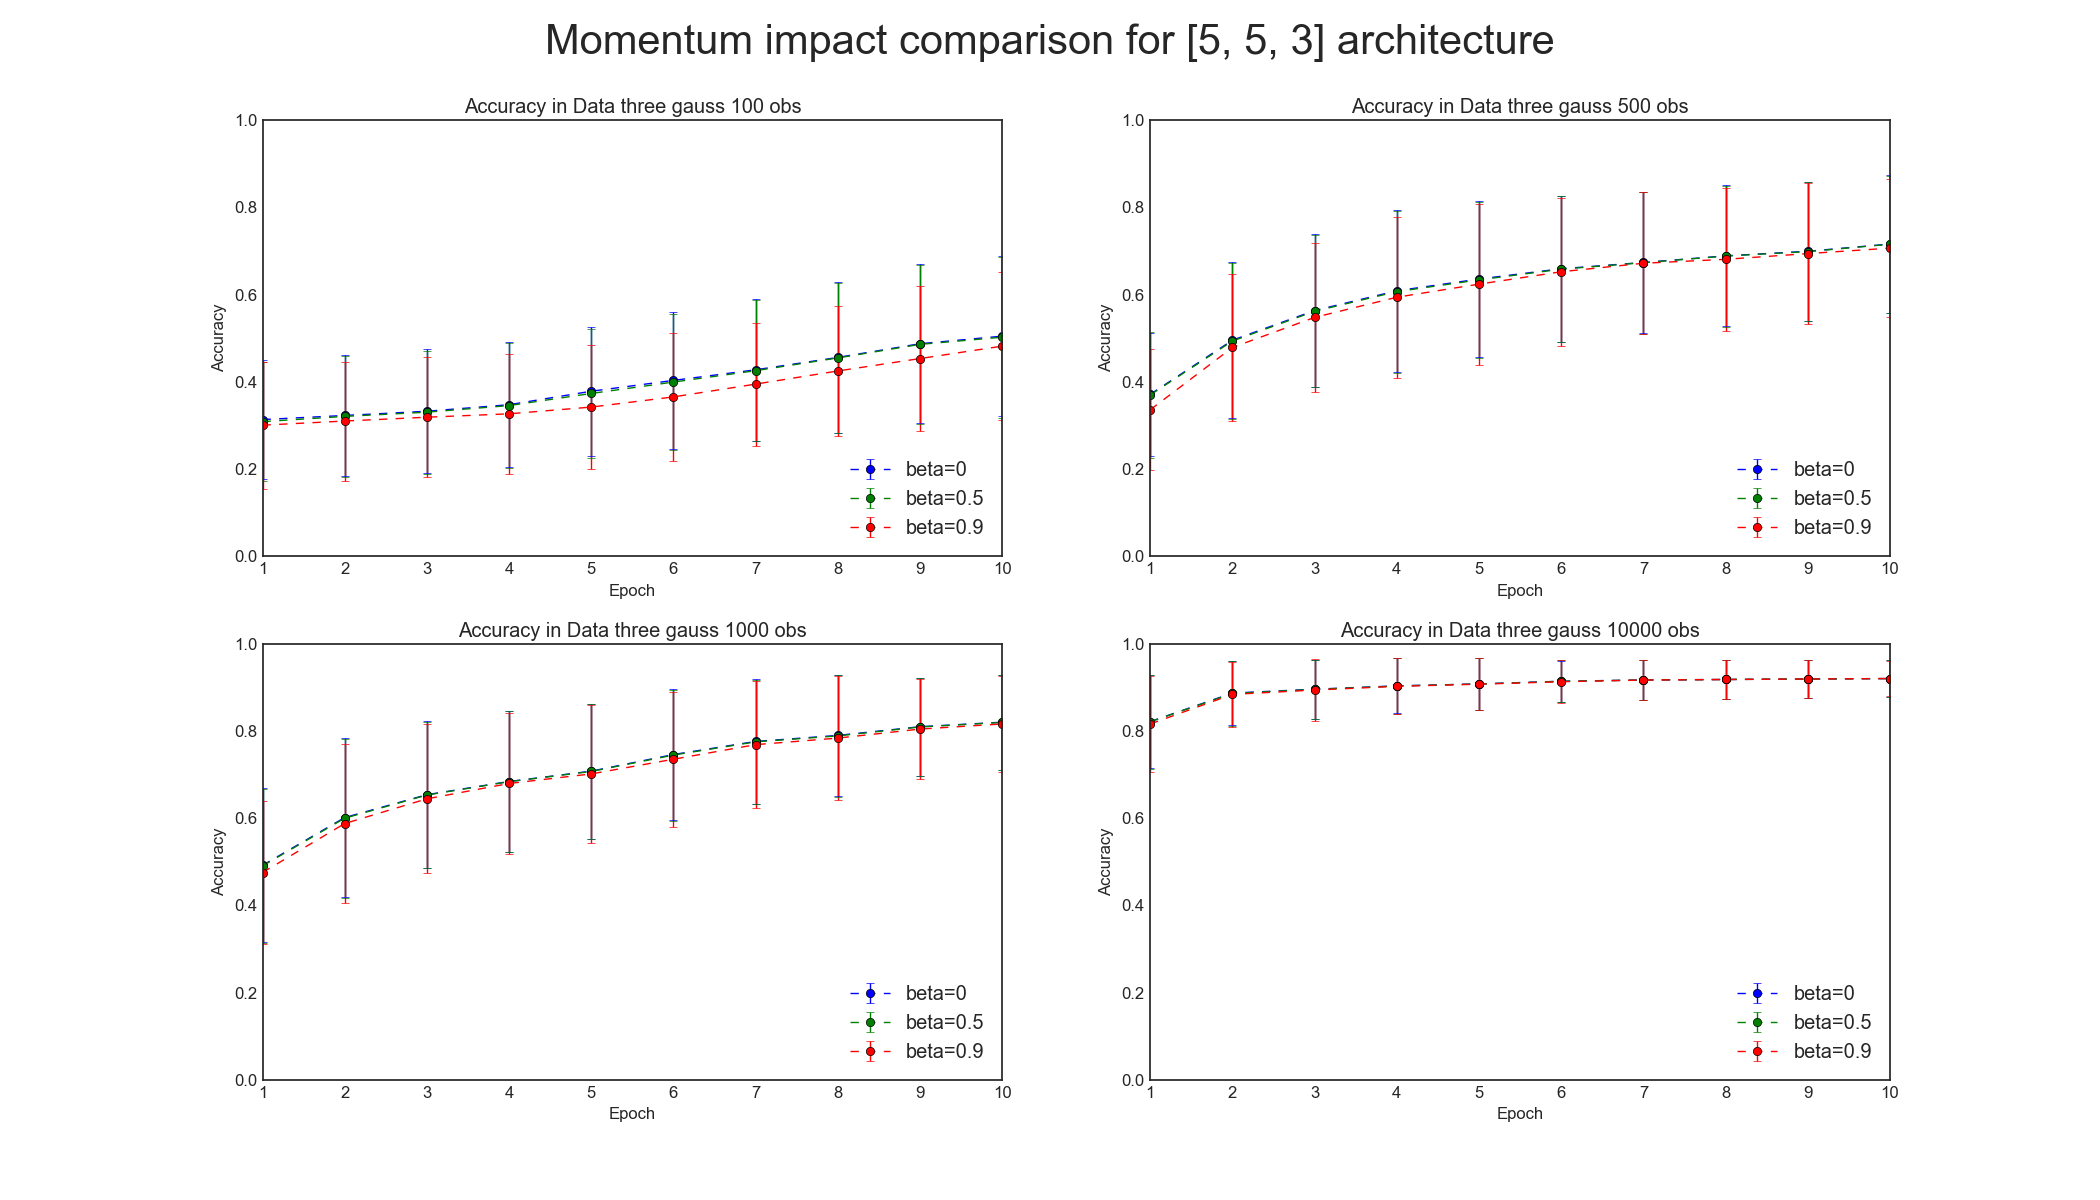
\includegraphics[width=1.4\textwidth]{results/classification/architecture-3/inertia_data_gauss_2020_03_24_09_27_18.png}}
   \caption{Mean accuracy achieved on the test set.}
\end{figure}


\centerline{
\begin{tabular}{llll}
\hline
{} &        beta=0 &      beta=0.5 &      beta=0.9 \\
\hline
Data three gauss 100 obs   &  0.50 +- 0.18 &  0.50 +- 0.18 &  0.48 +- 0.17 \\
Data three gauss 500 obs   &  0.72 +- 0.16 &  0.72 +- 0.16 &  0.71 +- 0.16 \\
Data three gauss 1000 obs  &  0.82 +- 0.11 &  0.82 +- 0.11 &  0.82 +- 0.11 \\
Data three gauss 10000 obs &  0.92 +- 0.04 &  0.92 +- 0.04 &  0.92 +- 0.04 \\
\hline
\end{tabular}
}

\newpage
% ----------------- BS ACTIVATION DATA  -------------------------
\begin{figure}[!ht]
    \noindent\makebox[\textwidth]{%
   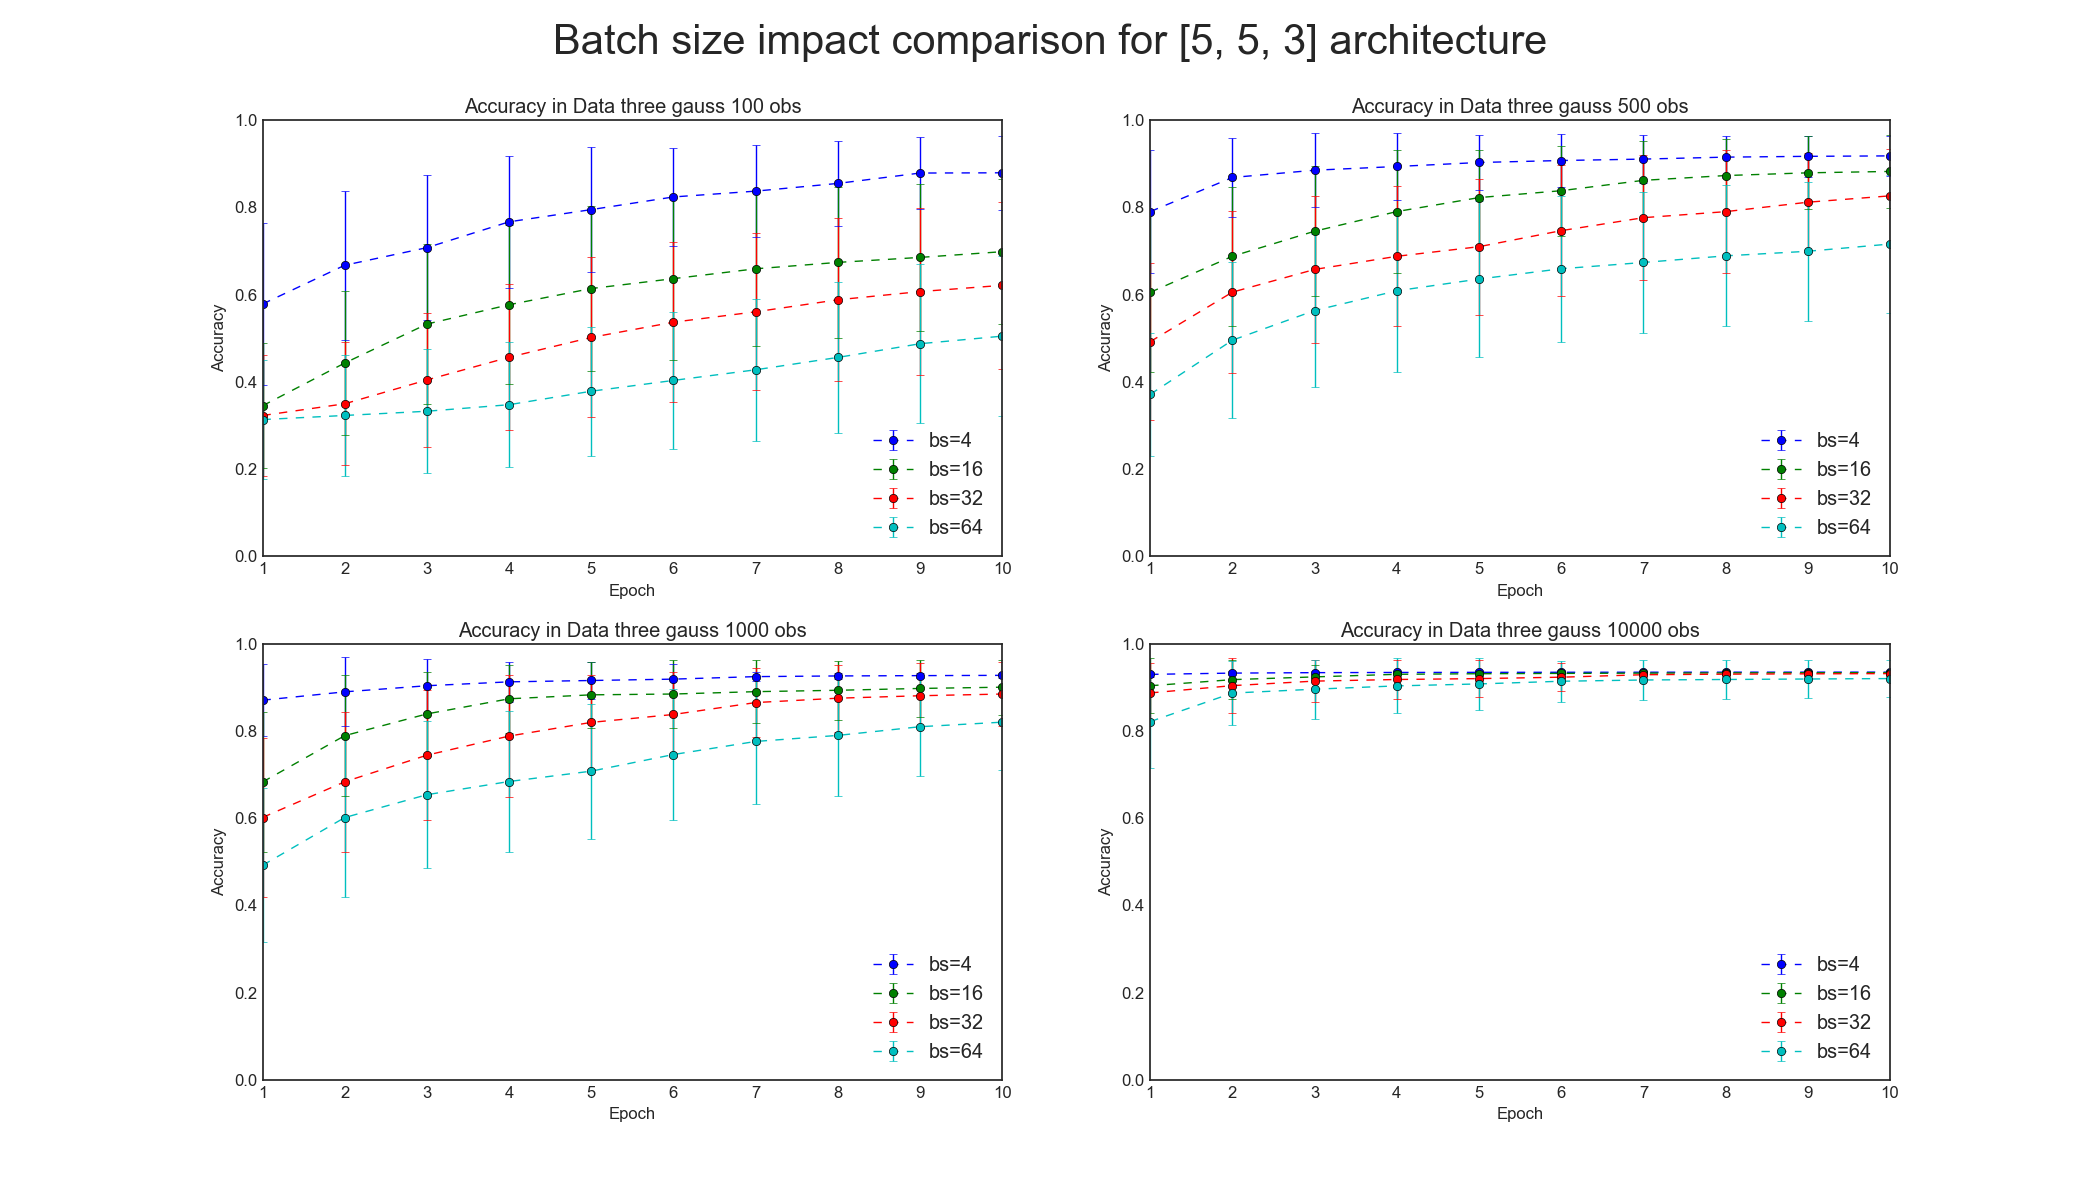
\includegraphics[width=1.4\textwidth]{results/classification/architecture-3/batch_size_data_gauss_2020_03_24_09_27_18.png}}
   \caption{Mean accuracy achieved on the test set.}
\end{figure}

\centerline{
\begin{tabular}{lllll}
\hline
{} &          bs=4 &         bs=16 &         bs=32 &         bs=64 \\
\hline
Data three gauss 100 obs   &  0.88 +- 0.08 &  0.70 +- 0.17 &  0.62 +- 0.19 &  0.50 +- 0.18 \\
Data three gauss 500 obs   &  0.92 +- 0.05 &  0.88 +- 0.08 &  0.83 +- 0.11 &  0.72 +- 0.16 \\
Data three gauss 1000 obs  &  0.93 +- 0.01 &  0.90 +- 0.06 &  0.88 +- 0.07 &  0.82 +- 0.11 \\
Data three gauss 10000 obs &  0.93 +- 0.00 &  0.93 +- 0.00 &  0.93 +- 0.01 &  0.92 +- 0.04 \\
\hline
\end{tabular}
}

\newpage
\subsubsection{Architecture 4}
\[[10, 5]\]
Two hidden layers, first with 10 neurons, second with 5 neurons.

% ----------------- LR ACTIVATION DATA  -------------------------

\begin{figure}[!ht]
    \noindent\makebox[\textwidth]{%
   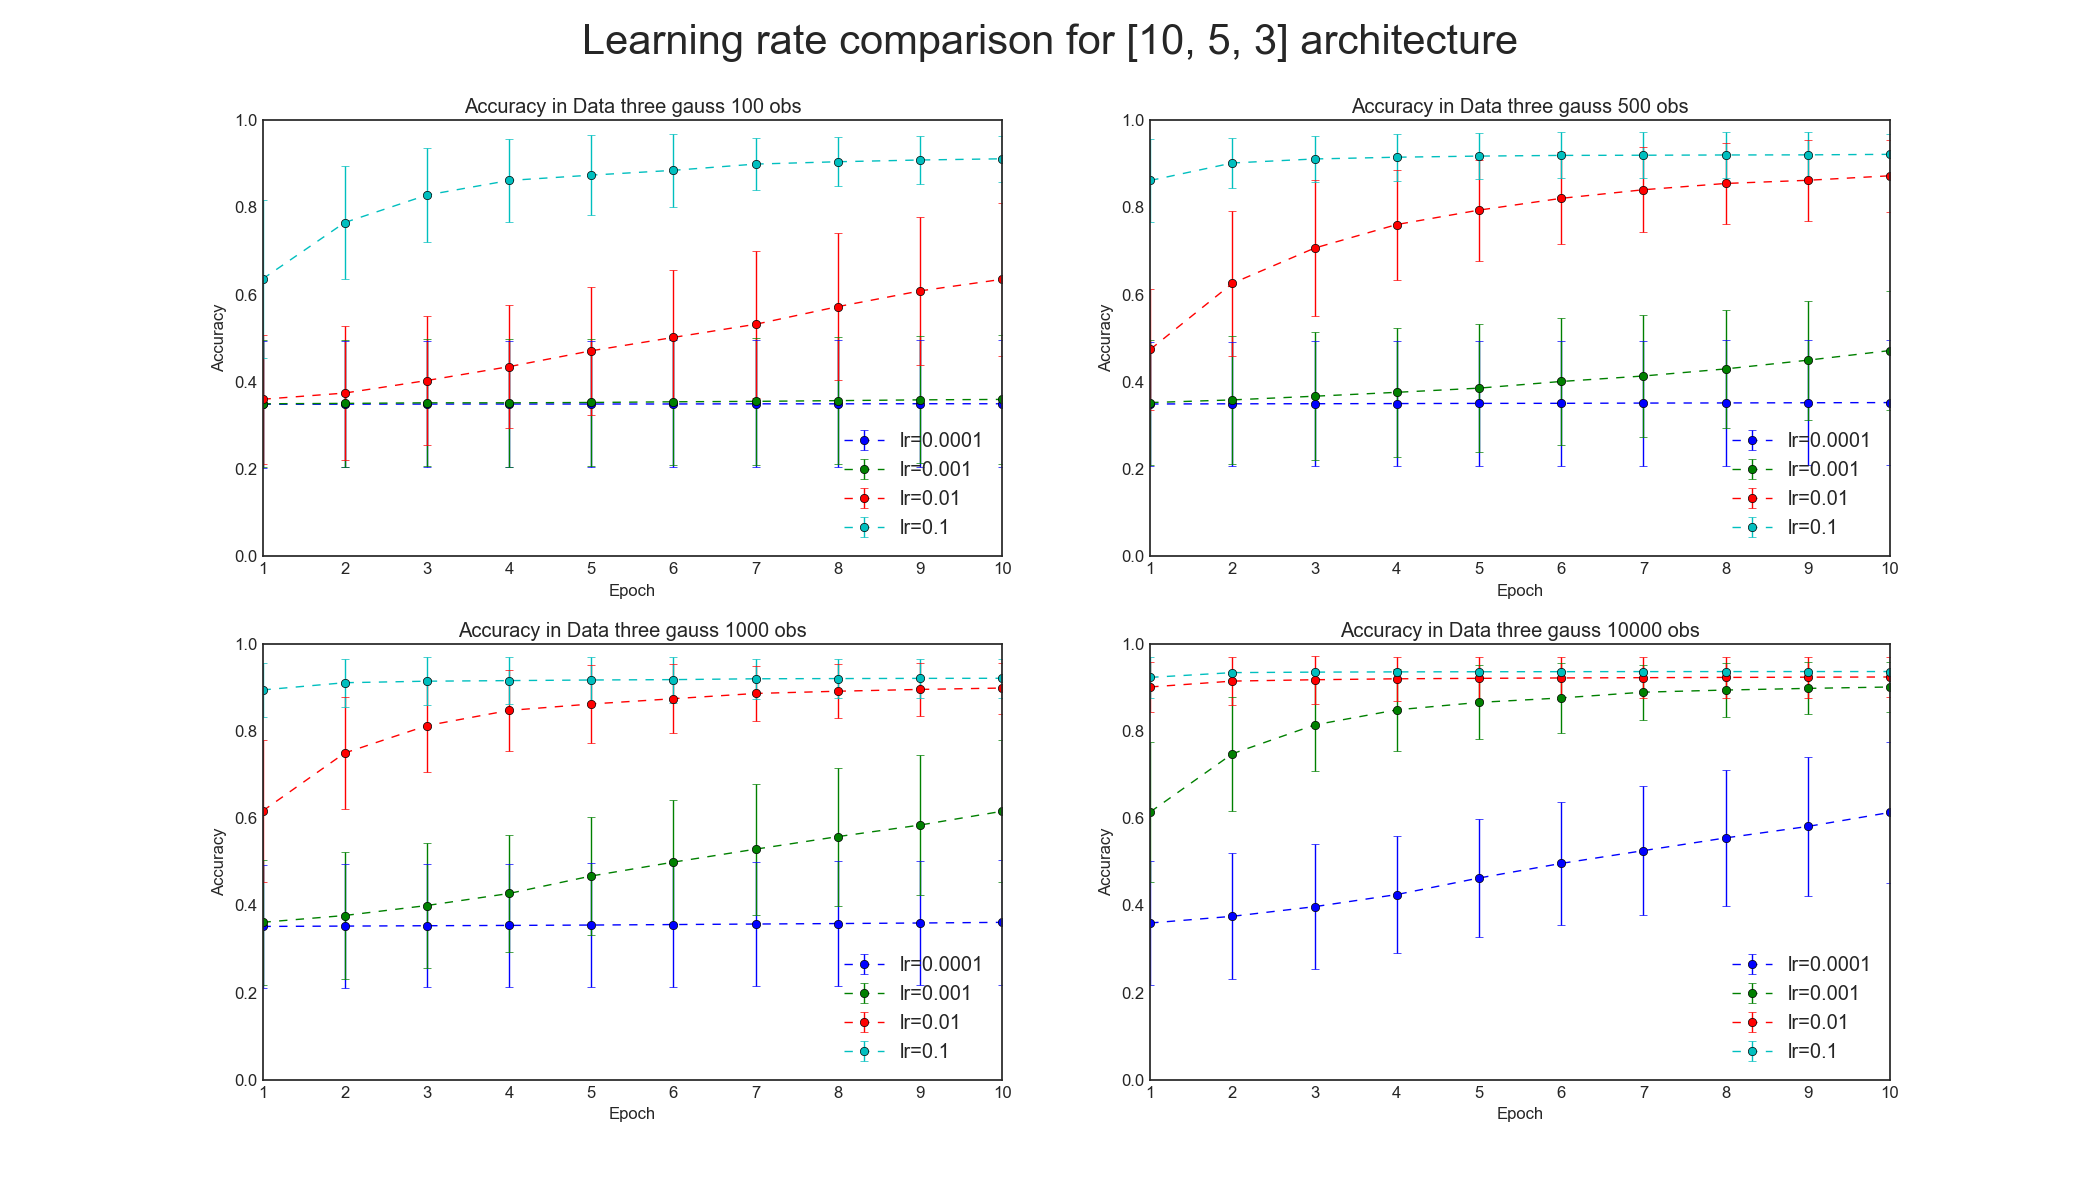
\includegraphics[width=1.4\textwidth]{results/classification/architecture-4/lr_data_gauss_2020_03_24_10_03_17.png}}
   \caption{Mean accuracy achieved on the test set.}
\end{figure}

\centerline{
\begin{tabular}{lllll}
\hline
{} &     lr=0.0001 &      lr=0.001 &       lr=0.01 &        lr=0.1 \\
\hline
Data three gauss 100 obs   &  0.35 +- 0.15 &  0.36 +- 0.15 &  0.64 +- 0.17 &  0.91 +- 0.05 \\
Data three gauss 500 obs   &  0.35 +- 0.14 &  0.47 +- 0.14 &  0.87 +- 0.08 &  0.92 +- 0.05 \\
Data three gauss 1000 obs  &  0.36 +- 0.14 &  0.62 +- 0.16 &  0.90 +- 0.06 &  0.92 +- 0.04 \\
Data three gauss 10000 obs &  0.61 +- 0.16 &  0.90 +- 0.06 &  0.92 +- 0.05 &  0.94 +- 0.00 \\
\hline
\end{tabular}
}

\newpage
% ----------------- AF ACTIVATION DATA  -------------------------
\begin{figure}[!ht]
    \noindent\makebox[\textwidth]{%
   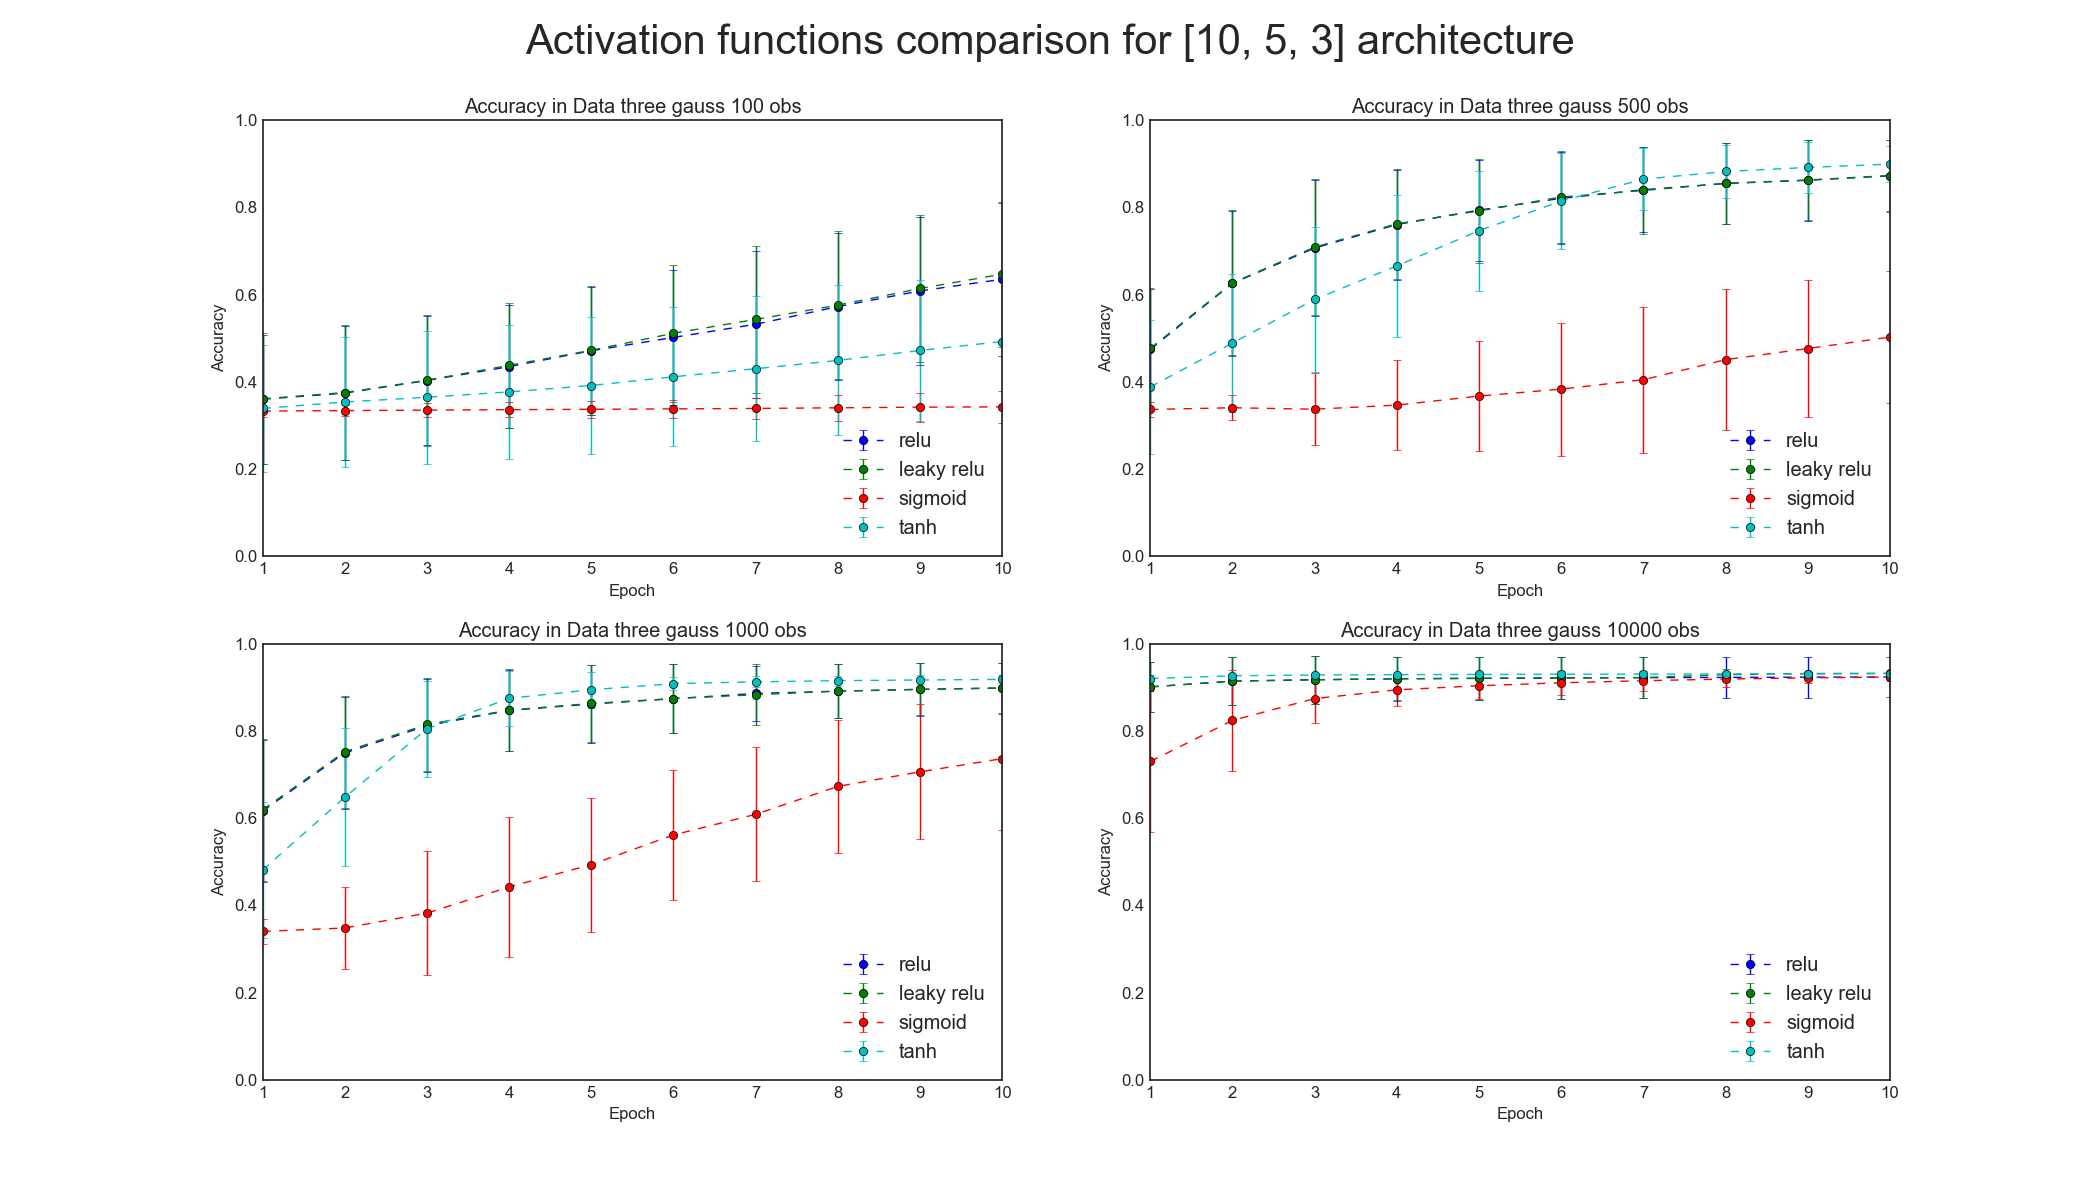
\includegraphics[width=1.4\textwidth]{results/classification/architecture-4/activation_function_data_gauss_2020_03_24_10_03_17.png}}
   \caption{Mean accuracy achieved on the test set.}
\end{figure}


\centerline{
\begin{tabular}{lllll}
\hline
{} &          relu &    leaky relu &       sigmoid &          tanh \\
\hline
Data three gauss 100 obs   &  0.64 +- 0.17 &  0.65 +- 0.17 &  0.34 +- 0.04 &  0.49 +- 0.16 \\
Data three gauss 500 obs   &  0.87 +- 0.08 &  0.87 +- 0.08 &  0.50 +- 0.15 &  0.90 +- 0.04 \\
Data three gauss 1000 obs  &  0.90 +- 0.06 &  0.90 +- 0.06 &  0.74 +- 0.16 &  0.92 +- 0.01 \\
Data three gauss 10000 obs &  0.92 +- 0.05 &  0.93 +- 0.00 &  0.92 +- 0.01 &  0.93 +- 0.00 \\
\hline
\end{tabular}
}

\newpage
% ----------------- INERTIA ACTIVATION DATA  -------------------------
\begin{figure}[!ht]
    \noindent\makebox[\textwidth]{%
   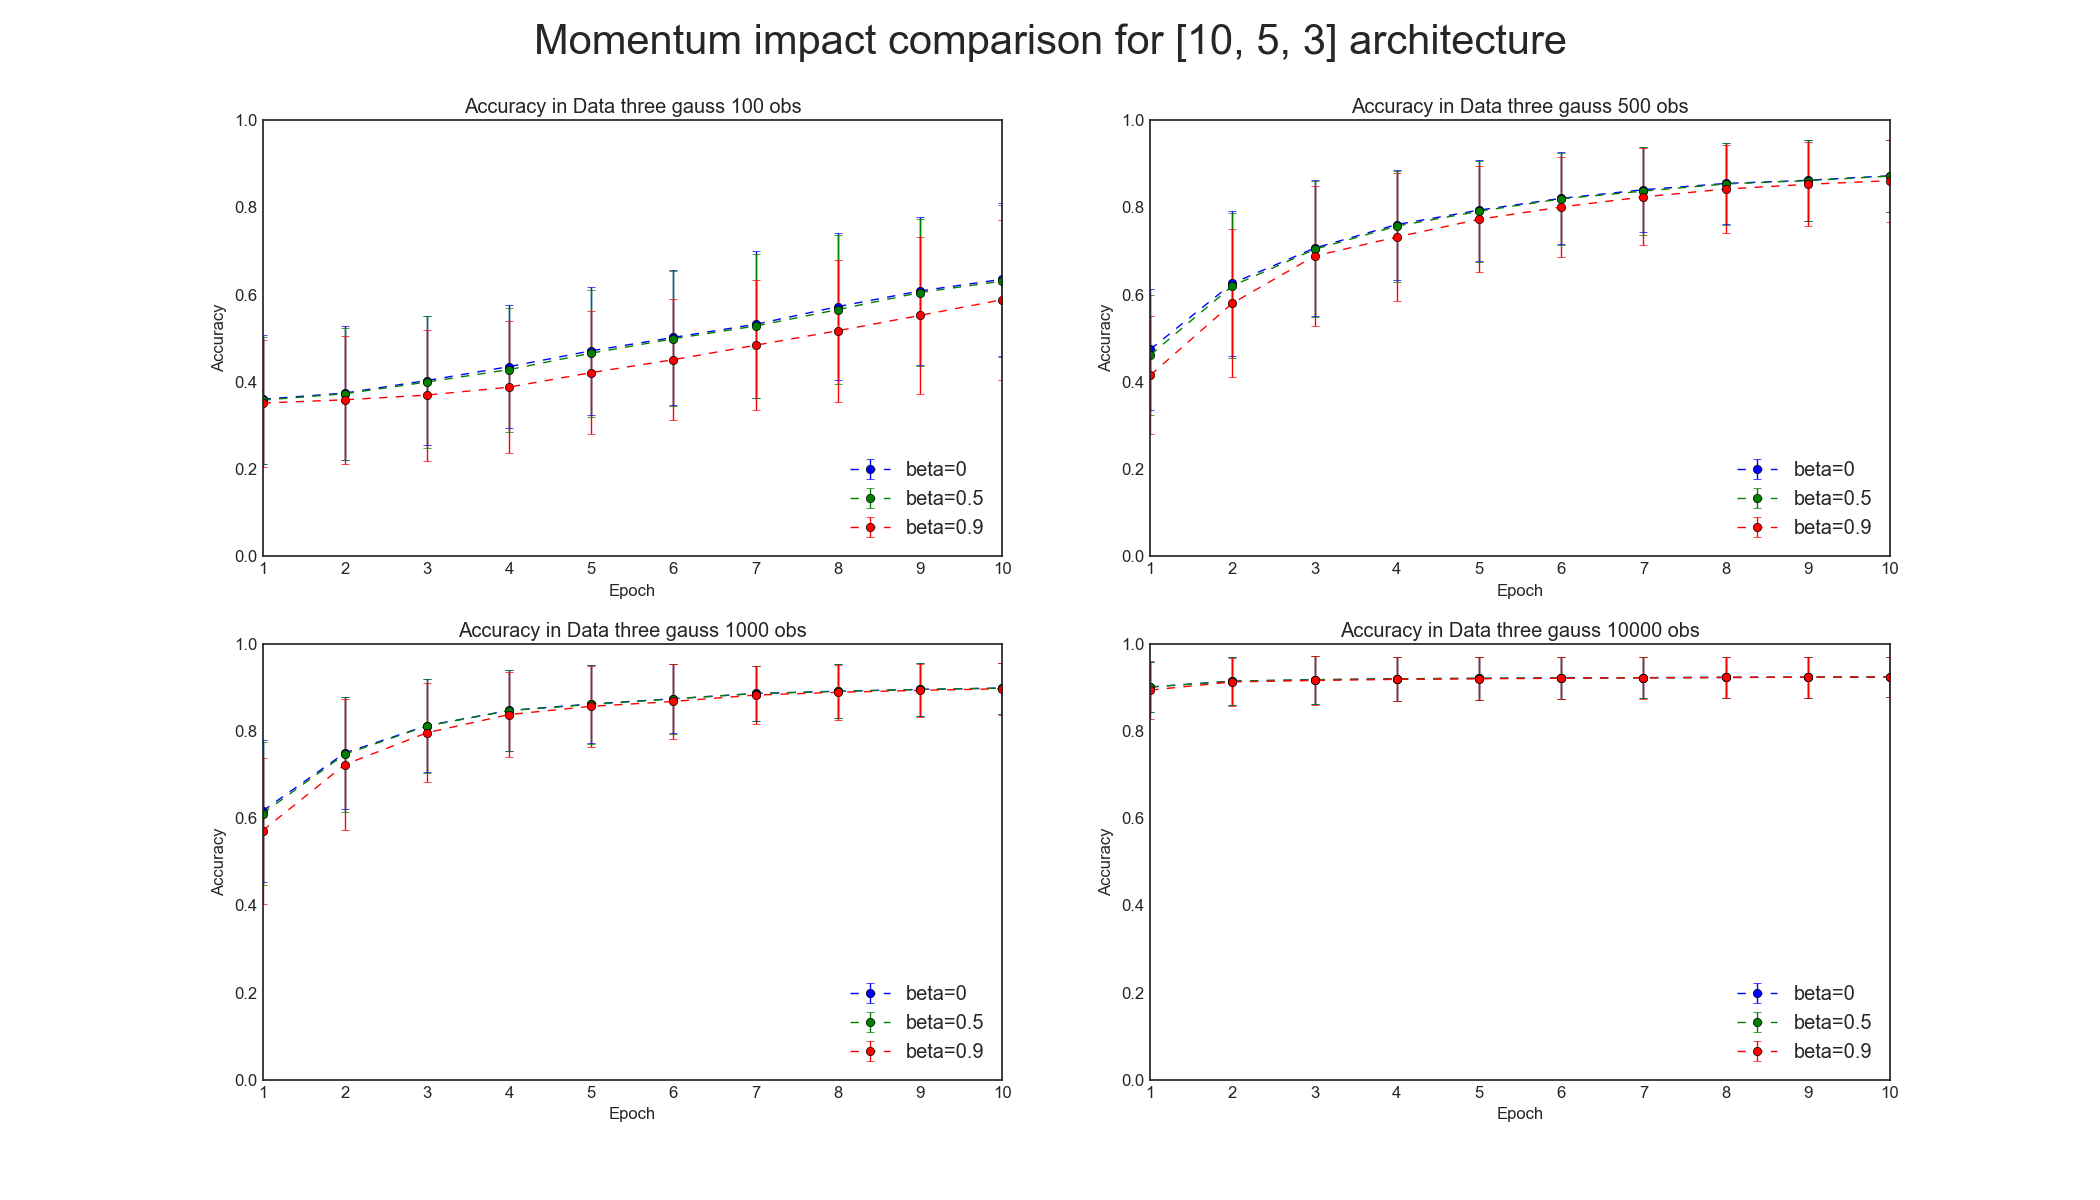
\includegraphics[width=1.4\textwidth]{results/classification/architecture-4/inertia_data_gauss_2020_03_24_10_03_18.png}}
   \caption{Mean accuracy achieved on the test set.}
\end{figure}


\centerline{
\begin{tabular}{llll}
\hline
{} &        beta=0 &      beta=0.5 &      beta=0.9 \\
\hline
Data three gauss 100 obs   &  0.64 +- 0.17 &  0.63 +- 0.17 &  0.59 +- 0.18 \\
Data three gauss 500 obs   &  0.87 +- 0.08 &  0.87 +- 0.08 &  0.86 +- 0.09 \\
Data three gauss 1000 obs  &  0.90 +- 0.06 &  0.90 +- 0.06 &  0.90 +- 0.06 \\
Data three gauss 10000 obs &  0.92 +- 0.05 &  0.92 +- 0.05 &  0.92 +- 0.05 \\
\hline
\end{tabular}
}

\newpage
% ----------------- BS ACTIVATION DATA  -------------------------
\begin{figure}[!ht]
    \noindent\makebox[\textwidth]{%
   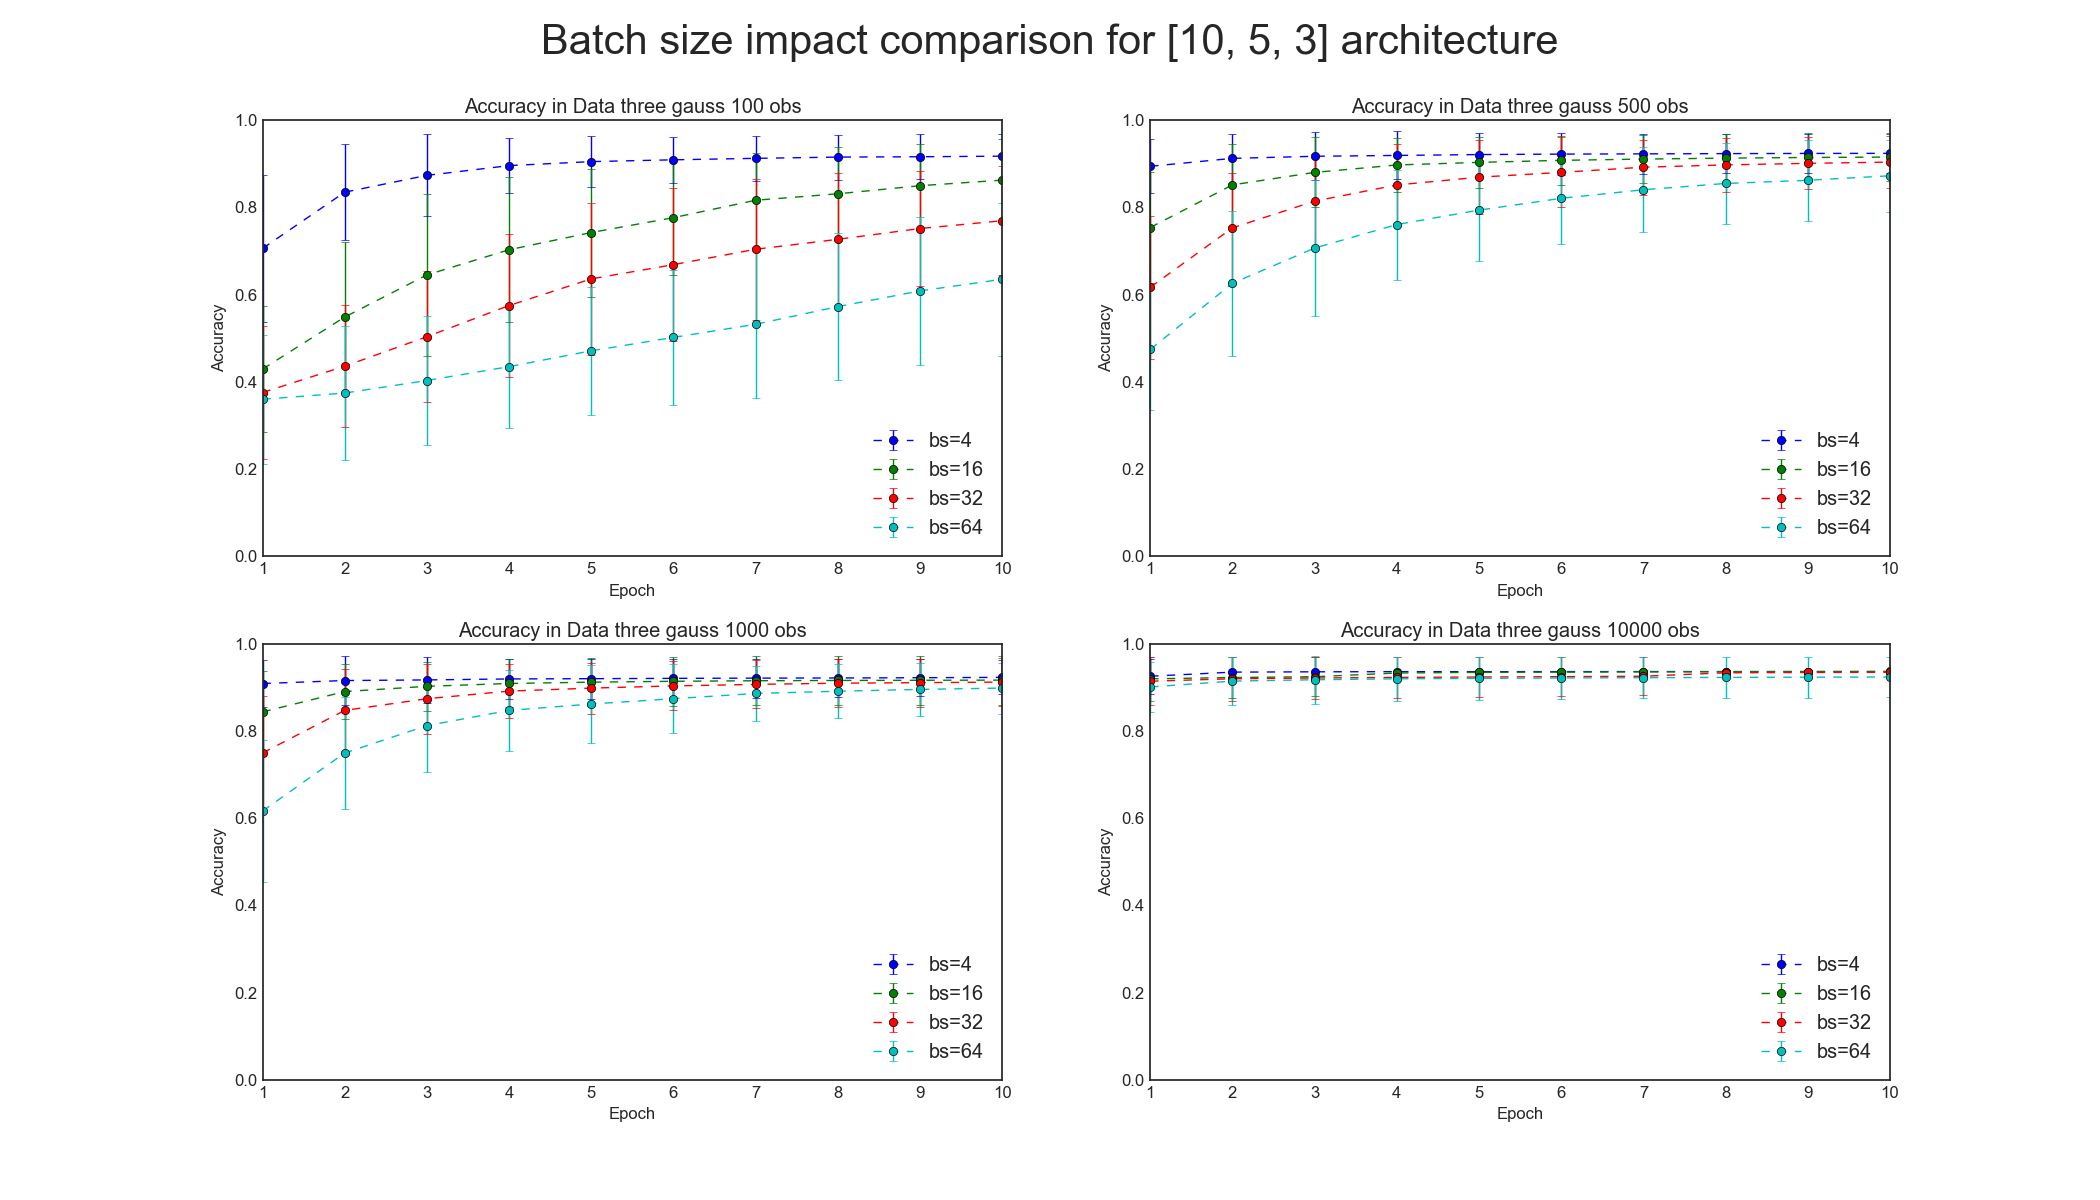
\includegraphics[width=1.4\textwidth]{results/classification/architecture-4/batch_size_data_gauss_2020_03_24_10_03_18.png}}
   \caption{Mean accuracy achieved on the test set.}
\end{figure}

\centerline{
\begin{tabular}{lllll}
\hline
{} &          bs=4 &         bs=16 &         bs=32 &         bs=64 \\
\hline
Data three gauss 100 obs   &  0.92 +- 0.05 &  0.86 +- 0.09 &  0.77 +- 0.12 &  0.64 +- 0.17 \\
Data three gauss 500 obs   &  0.92 +- 0.05 &  0.92 +- 0.06 &  0.90 +- 0.06 &  0.87 +- 0.08 \\
Data three gauss 1000 obs  &  0.92 +- 0.04 &  0.92 +- 0.06 &  0.91 +- 0.06 &  0.90 +- 0.06 \\
Data three gauss 10000 obs &  0.94 +- 0.00 &  0.94 +- 0.00 &  0.93 +- 0.00 &  0.92 +- 0.05 \\
\hline
\end{tabular}
}

\newpage
\subsubsection{Architecture 5}
\[[5, 5, 5, 5]\]
Four hidden layers, each with 5 neurons.

% ----------------- LR ACTIVATION DATA  -------------------------

\begin{figure}[!ht]
    \noindent\makebox[\textwidth]{%
   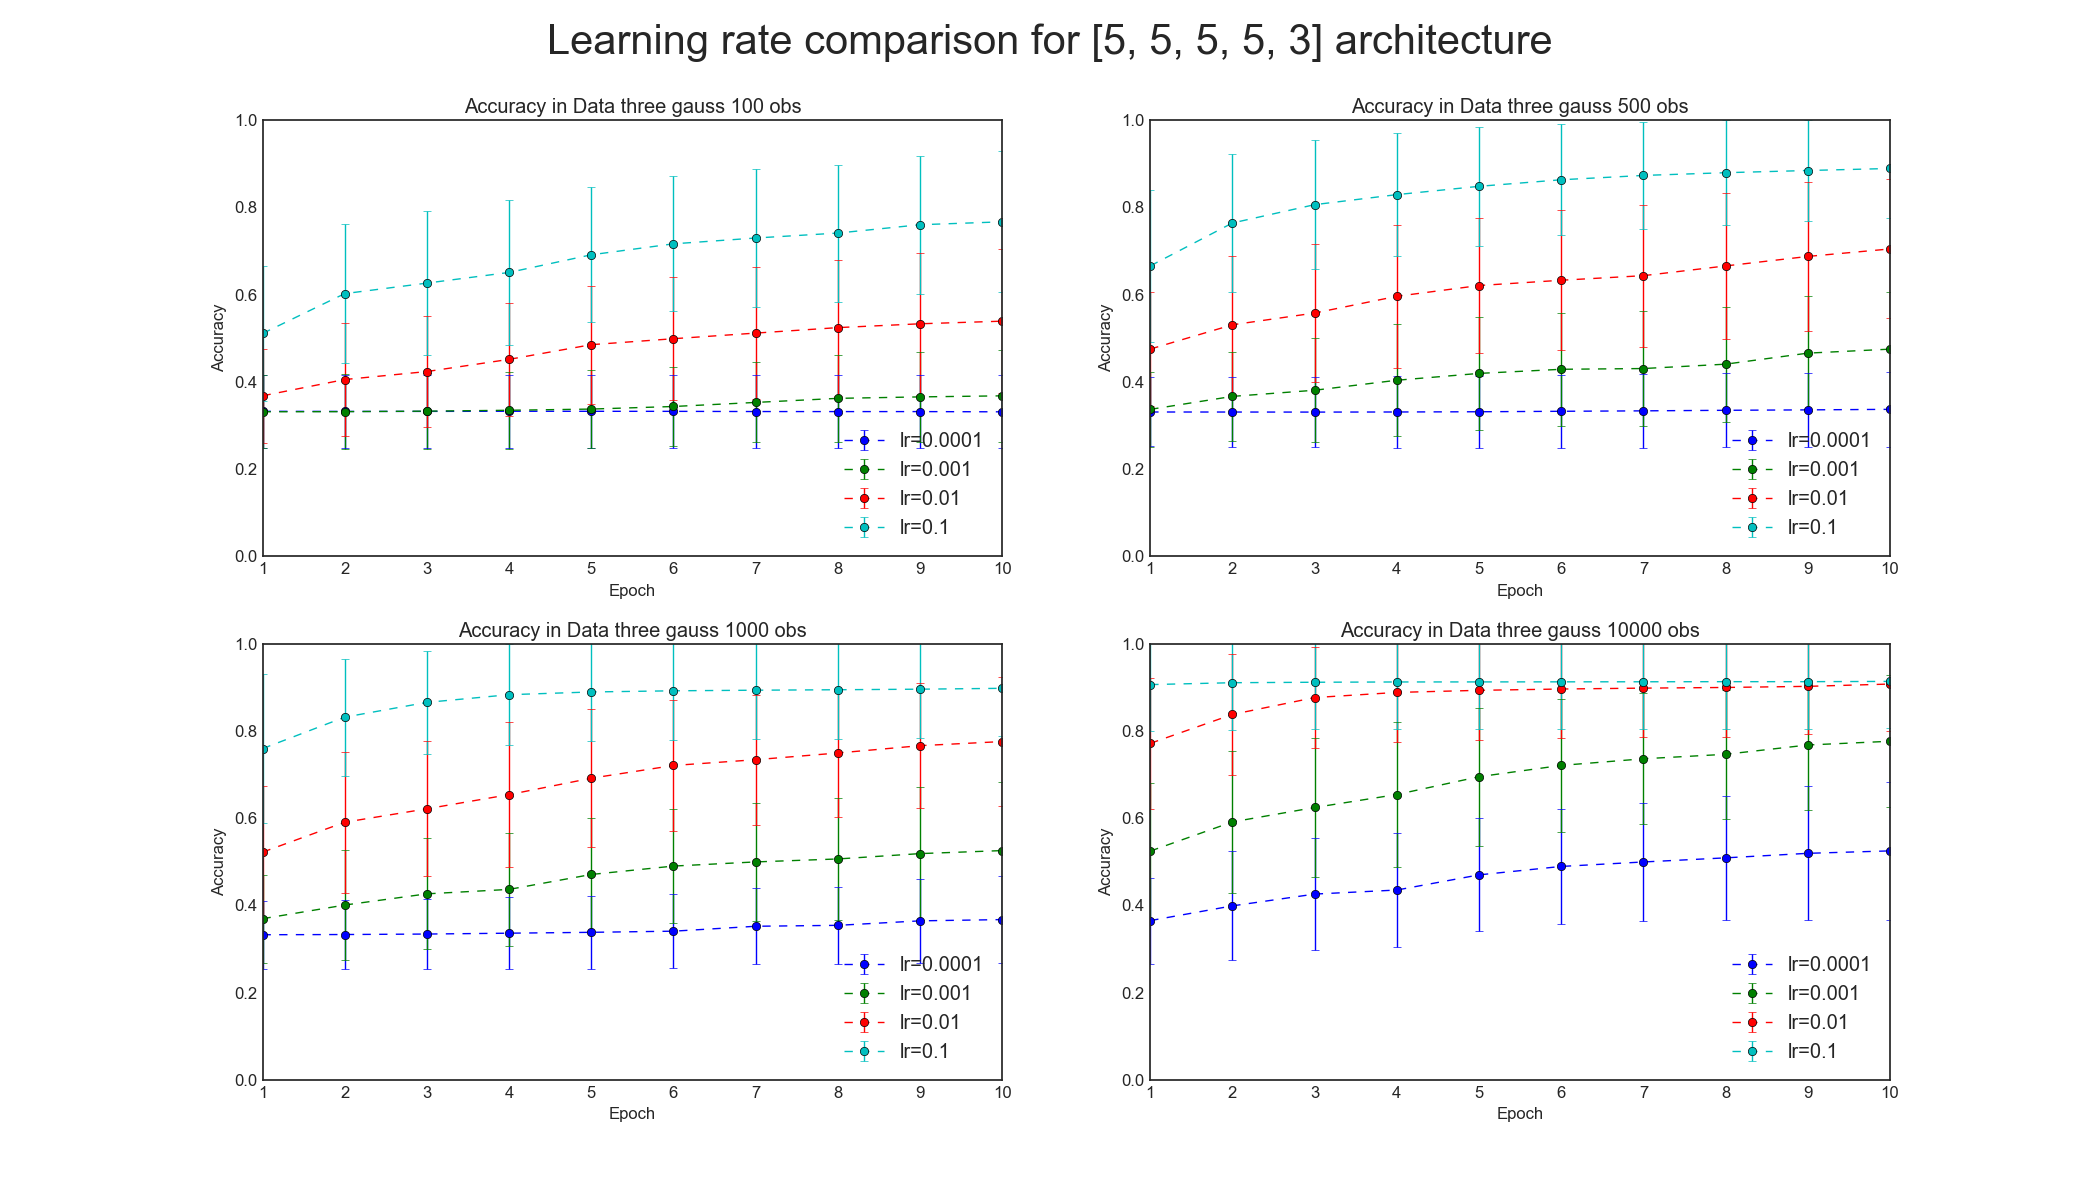
\includegraphics[width=1.4\textwidth]{results/classification/architecture-5/lr_data_gauss_2020_03_24_10_46_36.png}}
   \caption{Mean accuracy achieved on the test set.}
\end{figure}

\centerline{
\begin{tabular}{lllll}
\hline
{} &     lr=0.0001 &      lr=0.001 &       lr=0.01 &        lr=0.1 \\
\hline
Data three gauss 100 obs   &  0.33 +- 0.08 &  0.37 +- 0.11 &  0.54 +- 0.17 &  0.77 +- 0.16 \\
Data three gauss 500 obs   &  0.34 +- 0.09 &  0.47 +- 0.13 &  0.70 +- 0.16 &  0.89 +- 0.11 \\
Data three gauss 1000 obs  &  0.37 +- 0.10 &  0.53 +- 0.16 &  0.78 +- 0.15 &  0.90 +- 0.11 \\
Data three gauss 10000 obs &  0.53 +- 0.16 &  0.78 +- 0.15 &  0.91 +- 0.11 &  0.91 +- 0.11 \\
\hline
\end{tabular}
}

\newpage
% ----------------- AF ACTIVATION DATA  -------------------------
\begin{figure}[!ht]
    \noindent\makebox[\textwidth]{%
   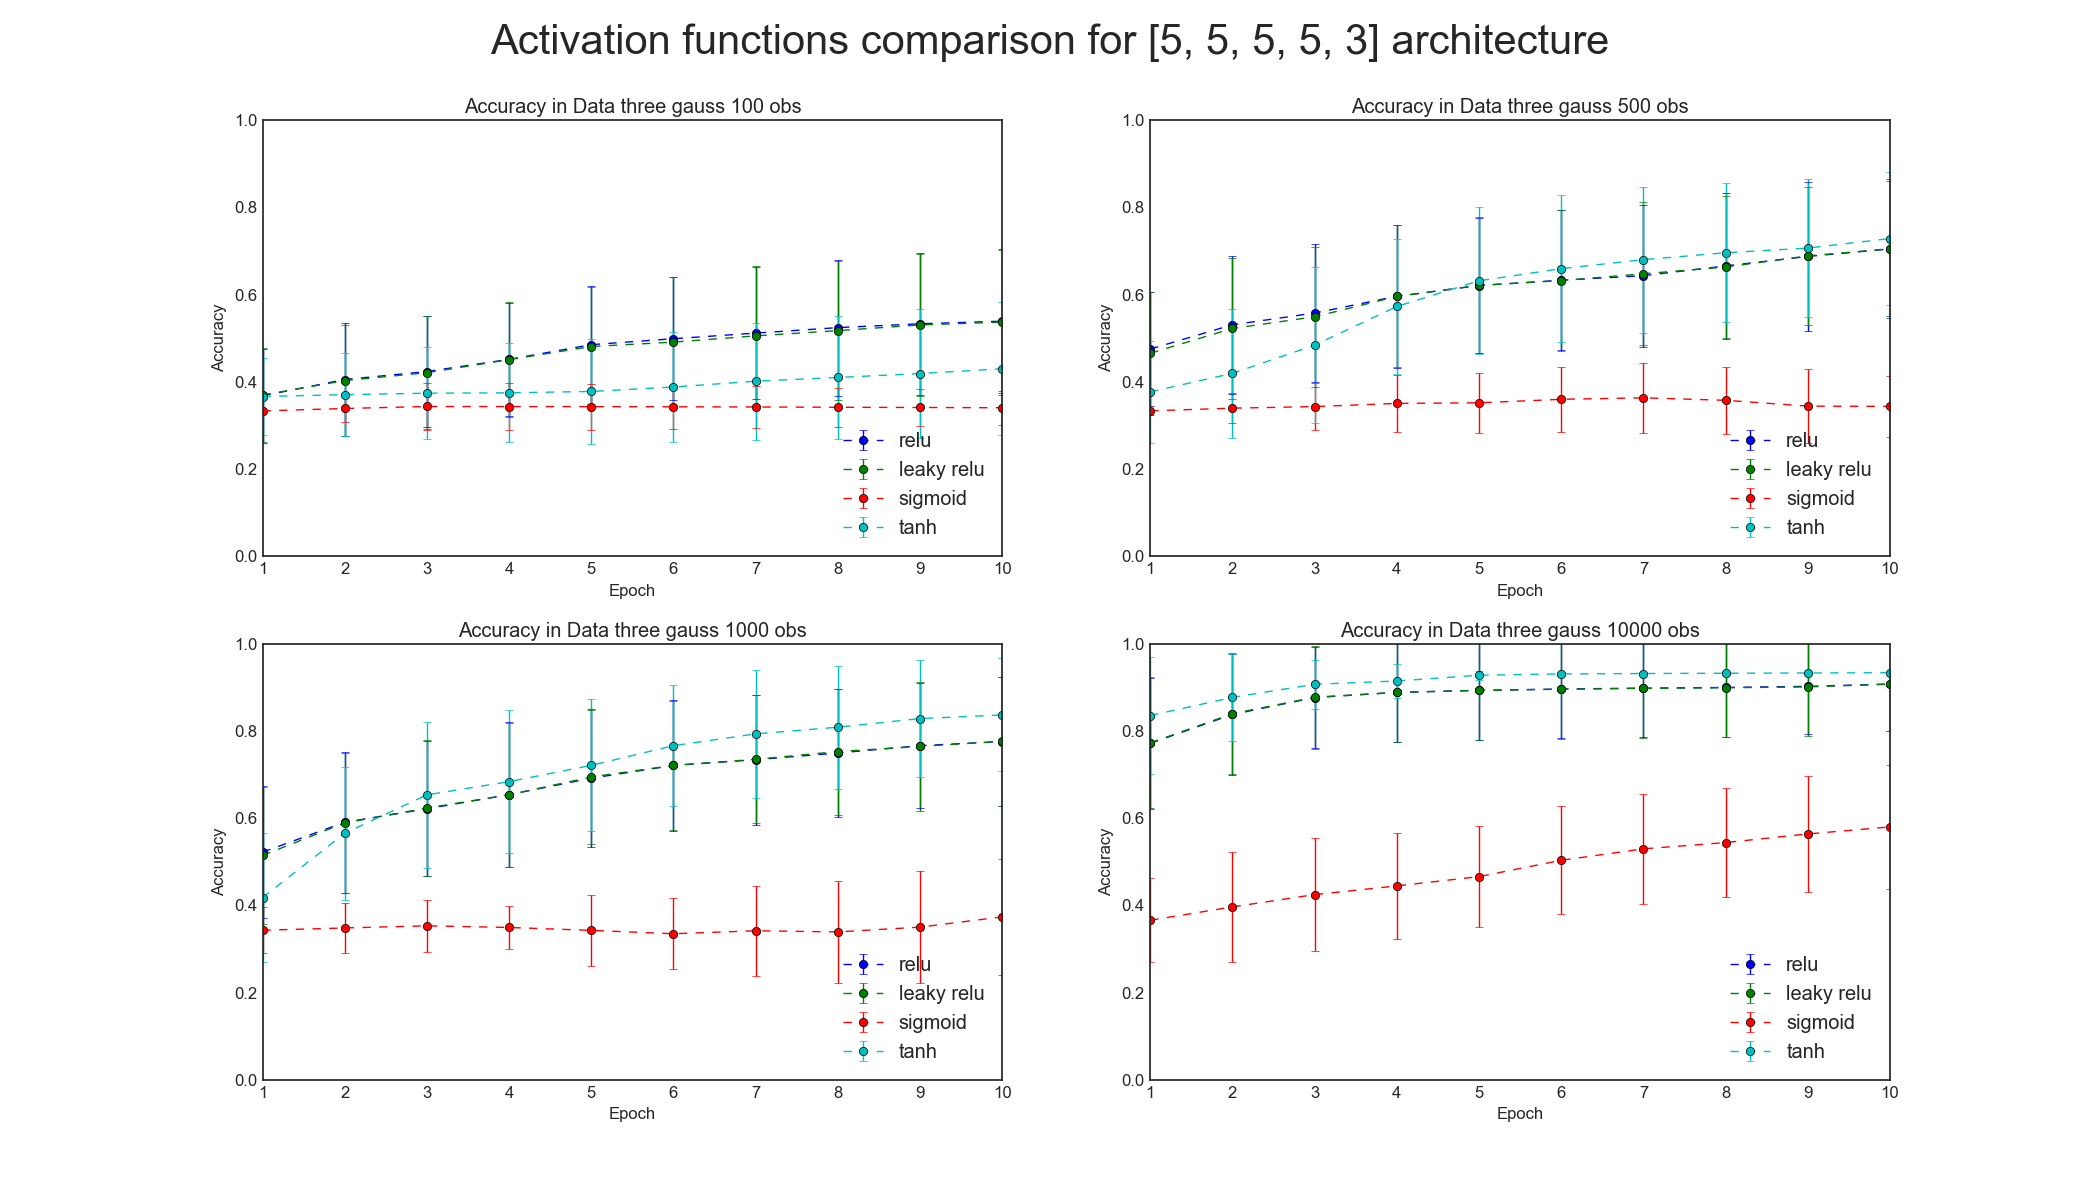
\includegraphics[width=1.4\textwidth]{results/classification/architecture-5/activation_function_data_gauss_2020_03_24_10_46_37.png}}
   \caption{Mean accuracy achieved on the test set.}
\end{figure}


\centerline{
\begin{tabular}{lllll}
\hline
{} &          relu &    leaky relu &       sigmoid &          tanh \\
\hline
Data three gauss 100 obs   &  0.54 +- 0.17 &  0.54 +- 0.17 &  0.34 +- 0.05 &  0.43 +- 0.15 \\
Data three gauss 500 obs   &  0.70 +- 0.16 &  0.70 +- 0.15 &  0.36 +- 0.08 &  0.73 +- 0.15 \\
Data three gauss 1000 obs  &  0.78 +- 0.15 &  0.78 +- 0.15 &  0.37 +- 0.13 &  0.84 +- 0.13 \\
Data three gauss 10000 obs &  0.91 +- 0.11 &  0.91 +- 0.11 &  0.58 +- 0.14 &  0.93 +- 0.00 \\
\hline
\end{tabular}
}


\newpage
% ----------------- INERTIA ACTIVATION DATA  -------------------------
\begin{figure}[!ht]
    \noindent\makebox[\textwidth]{%
   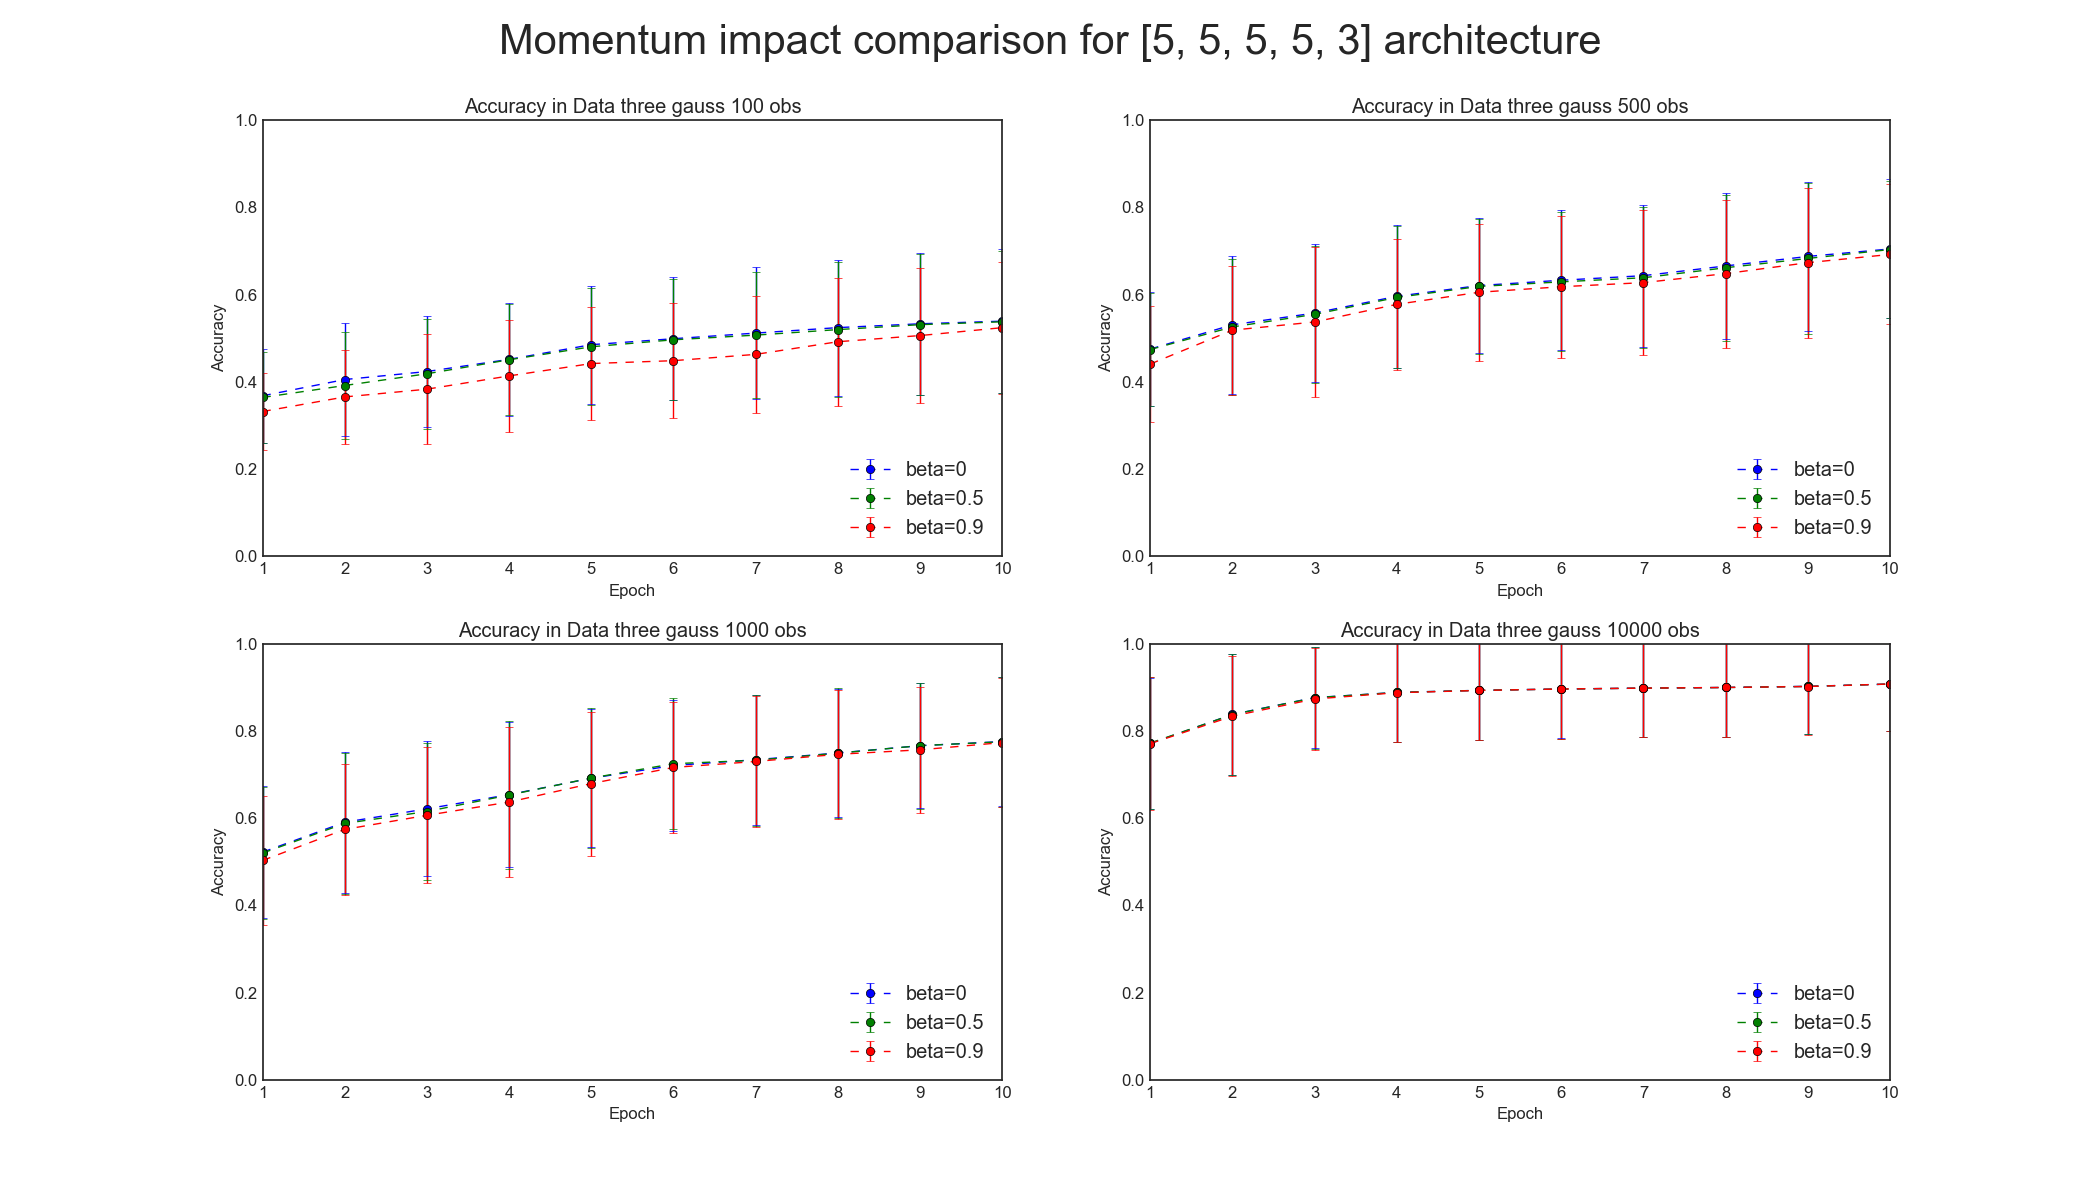
\includegraphics[width=1.4\textwidth]{results/classification/architecture-5/inertia_data_gauss_2020_03_24_10_46_37.png}}
   \caption{Mean accuracy achieved on the test set.}
\end{figure}


\centerline{
\begin{tabular}{llll}
\hline
{} &        beta=0 &      beta=0.5 &      beta=0.9 \\
\hline
Data three gauss 100 obs   &  0.54 +- 0.17 &  0.54 +- 0.16 &  0.52 +- 0.15 \\
Data three gauss 500 obs   &  0.70 +- 0.16 &  0.70 +- 0.16 &  0.69 +- 0.16 \\
Data three gauss 1000 obs  &  0.78 +- 0.15 &  0.78 +- 0.15 &  0.77 +- 0.15 \\
Data three gauss 10000 obs &  0.91 +- 0.11 &  0.91 +- 0.11 &  0.91 +- 0.11 \\
\hline
\end{tabular}
}

\newpage
% ----------------- BS ACTIVATION DATA  -------------------------
\begin{figure}[!ht]
    \noindent\makebox[\textwidth]{%
   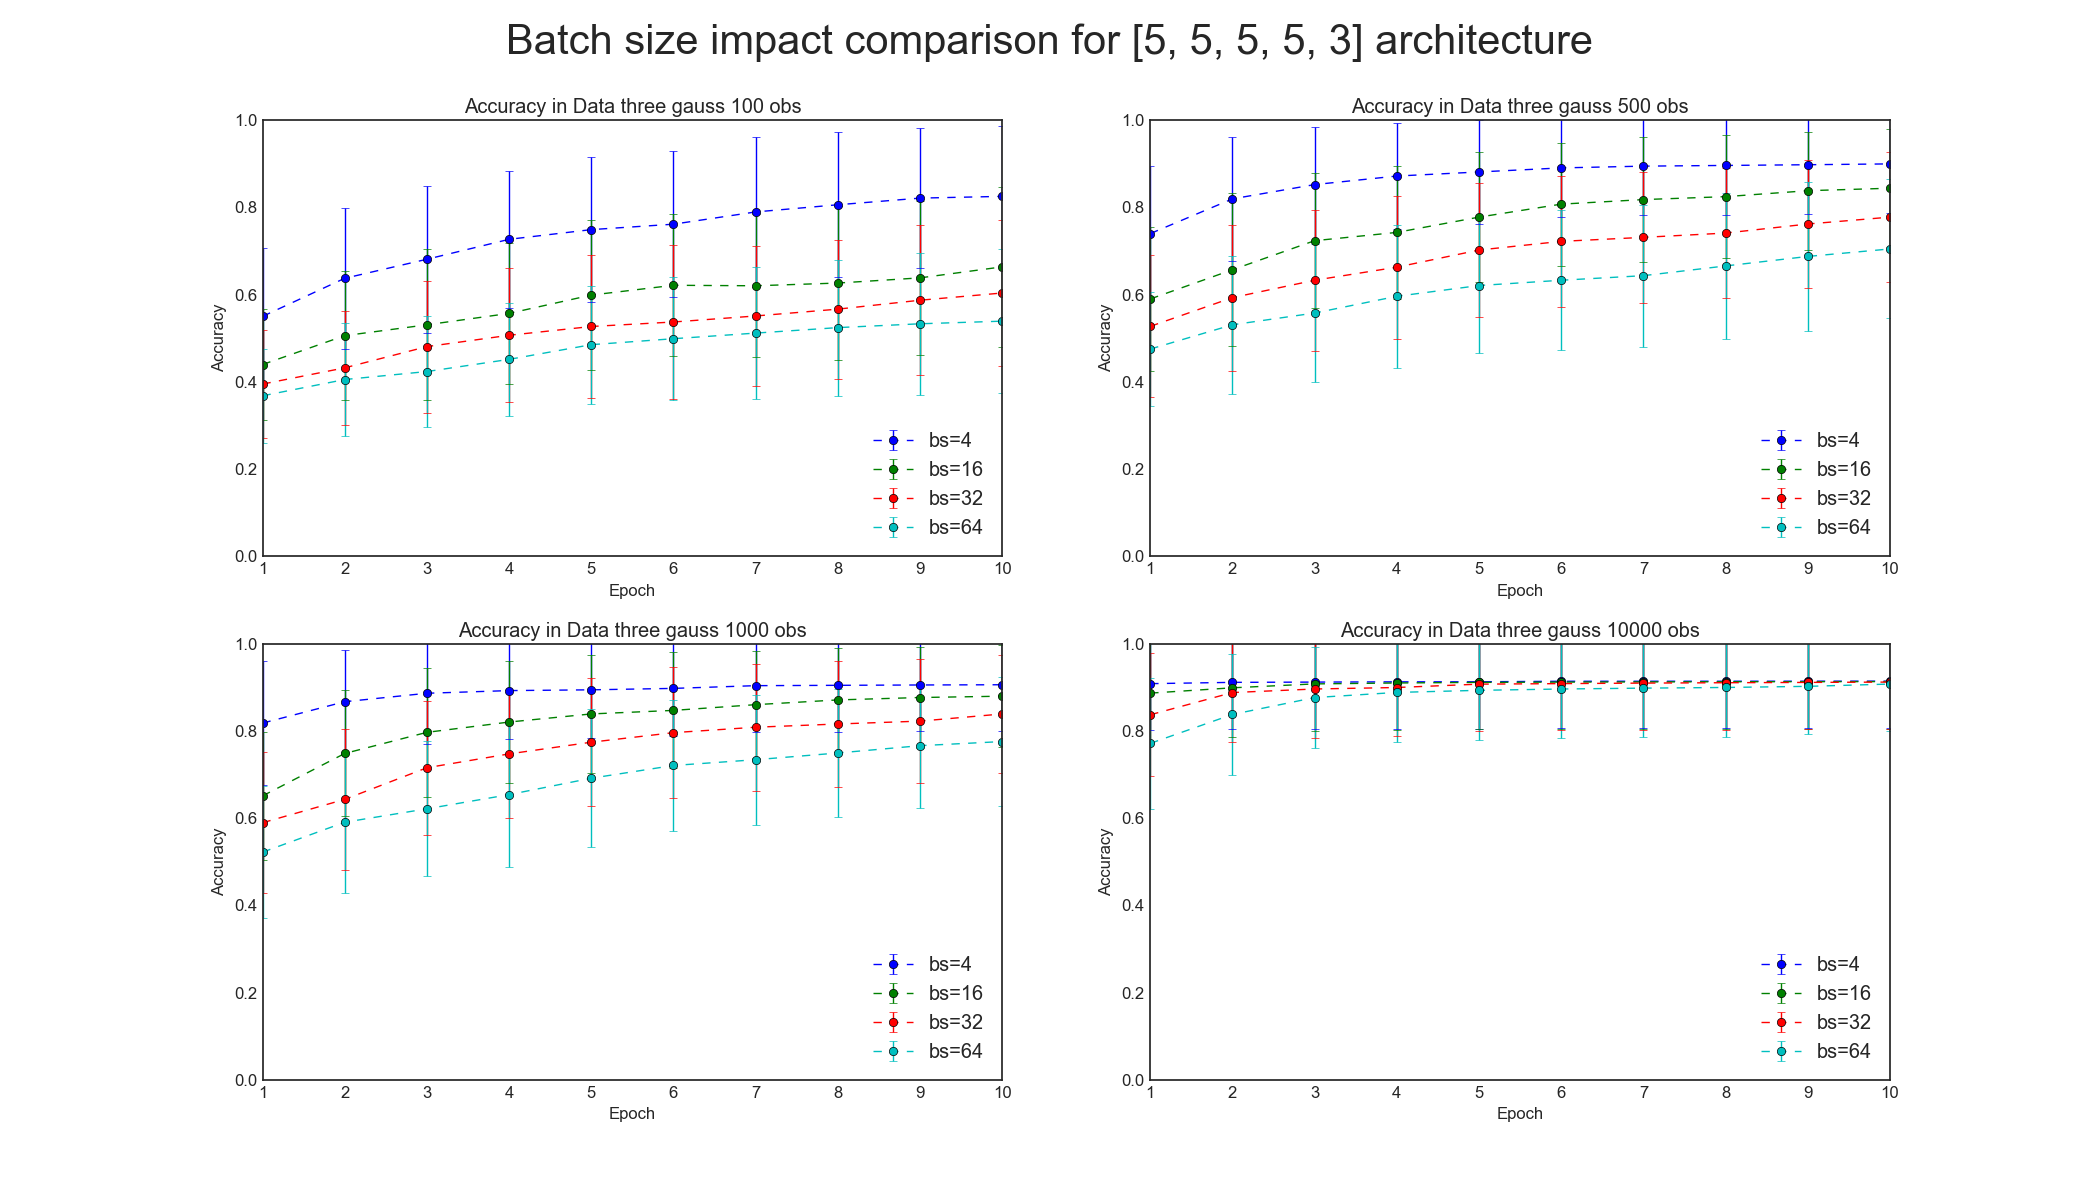
\includegraphics[width=1.4\textwidth]{results/classification/architecture-5/batch_size_data_gauss_2020_03_24_10_46_38.png}}
   \caption{Mean accuracy achieved on the test set.}
\end{figure}

\centerline{
\begin{tabular}{lllll}
\hline
{} &          bs=4 &         bs=16 &         bs=32 &         bs=64 \\
\hline
Data three gauss 100 obs   &  0.82 +- 0.16 &  0.66 +- 0.18 &  0.60 +- 0.17 &  0.54 +- 0.17 \\
Data three gauss 500 obs   &  0.90 +- 0.11 &  0.84 +- 0.13 &  0.78 +- 0.15 &  0.70 +- 0.16 \\
Data three gauss 1000 obs  &  0.91 +- 0.11 &  0.88 +- 0.12 &  0.84 +- 0.13 &  0.78 +- 0.15 \\
Data three gauss 10000 obs &  0.91 +- 0.11 &  0.91 +- 0.11 &  0.91 +- 0.11 &  0.91 +- 0.11 \\
\hline
\end{tabular}
}



\newpage
\subsubsection{Architecture 6}
\[[10, 10, 5, 5]\]
Four hidden layers, first two with 10 neurons each, next two with 5 neurons each.

% ----------------- LR ACTIVATION DATA  -------------------------

\begin{figure}[!ht]
    \noindent\makebox[\textwidth]{%
   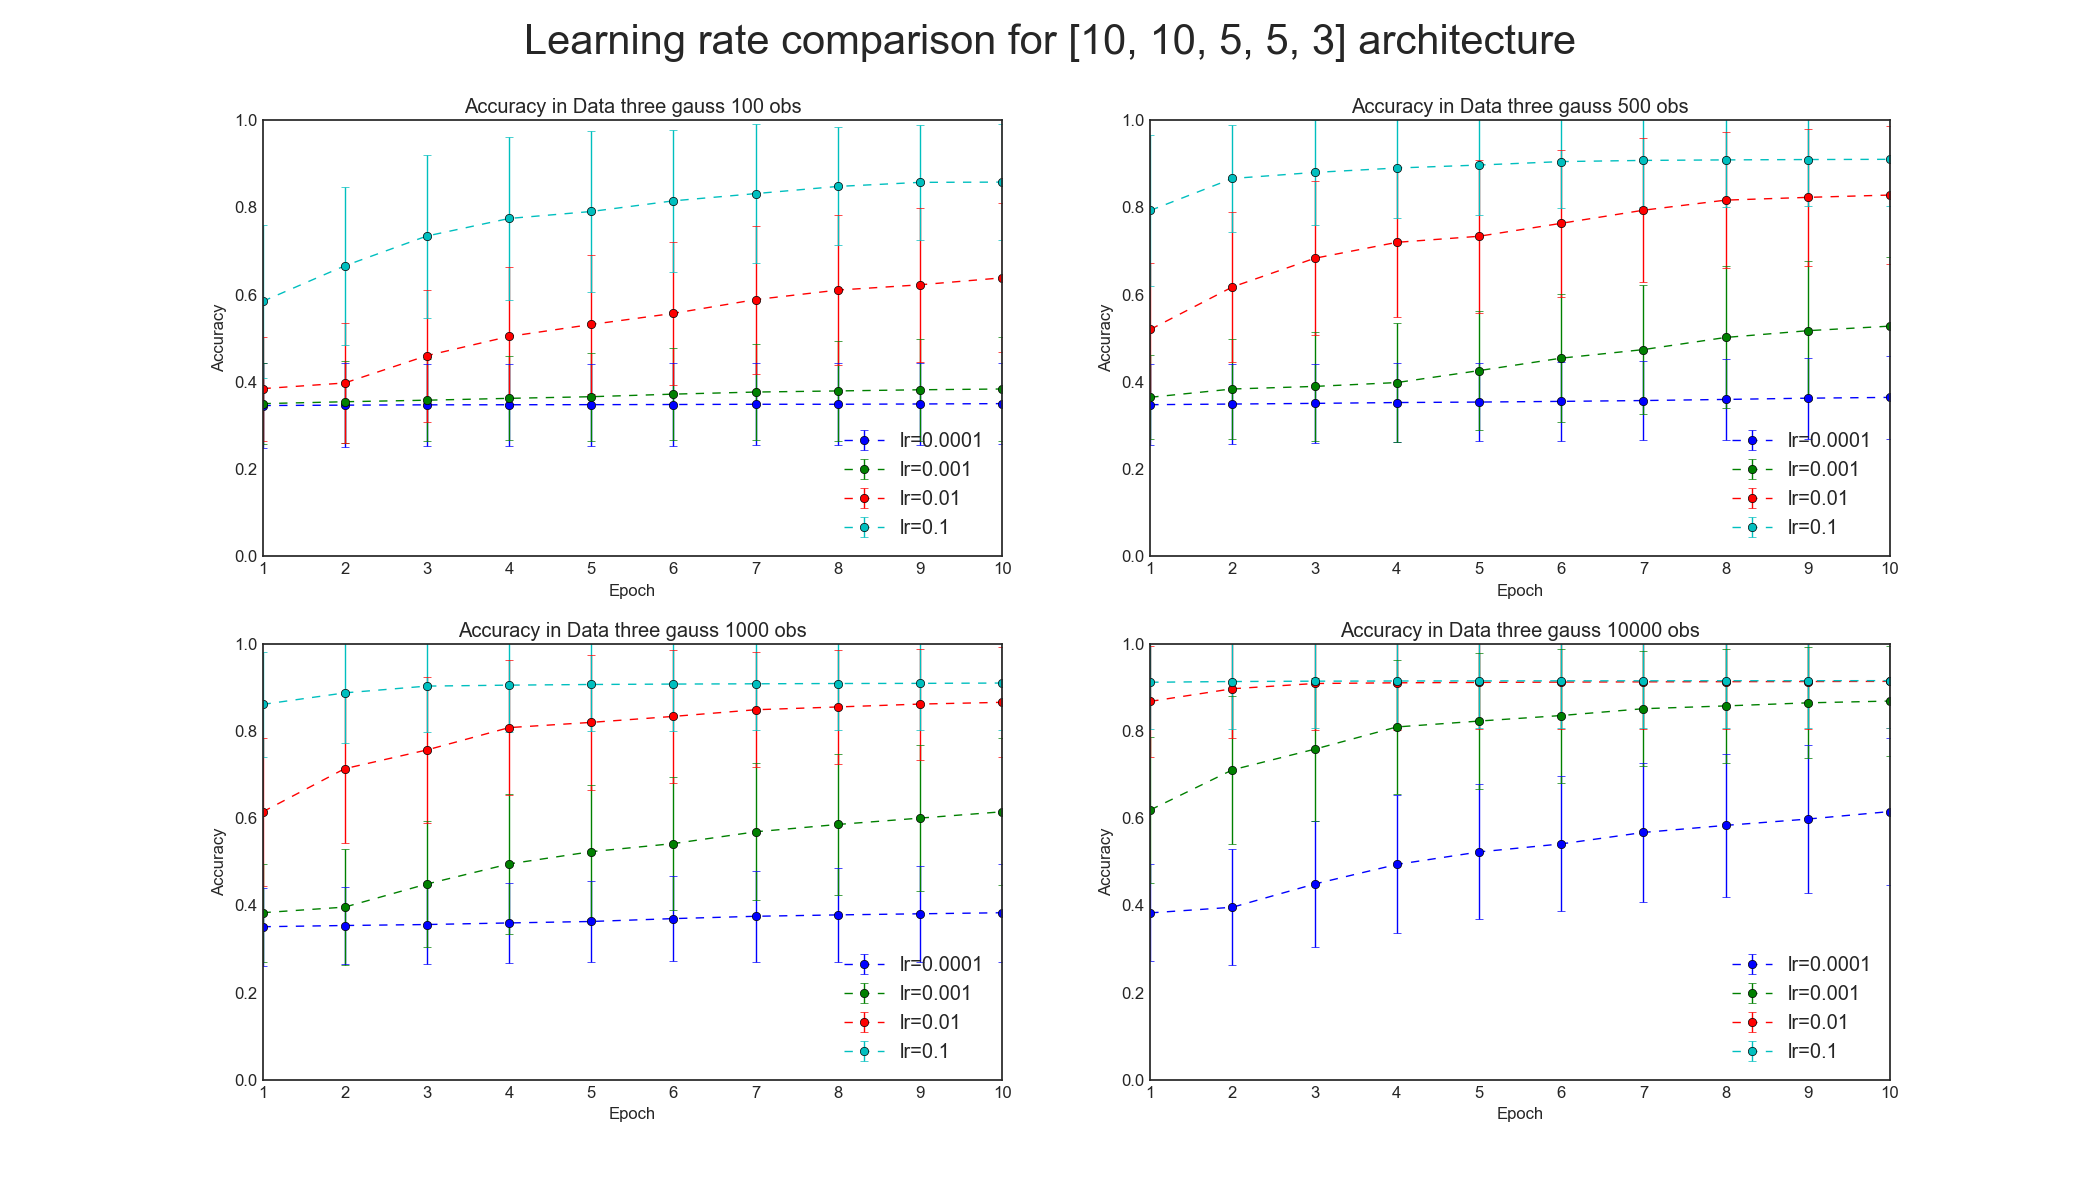
\includegraphics[width=1.4\textwidth]{results/classification/architecture-6/lr_data_gauss_2020_03_24_11_31_45.png}}
\end{figure}

\centerline{
\begin{tabular}{lllll}
\hline
{} &     lr=0.0001 &      lr=0.001 &       lr=0.01 &        lr=0.1 \\
\hline
Data three gauss 100 obs   &  0.35 +- 0.09 &  0.38 +- 0.12 &  0.64 +- 0.17 &  0.86 +- 0.13 \\
Data three gauss 500 obs   &  0.36 +- 0.10 &  0.53 +- 0.16 &  0.83 +- 0.16 &  0.91 +- 0.11 \\
Data three gauss 1000 obs  &  0.38 +- 0.11 &  0.61 +- 0.17 &  0.87 +- 0.13 &  0.91 +- 0.11 \\
Data three gauss 10000 obs &  0.62 +- 0.17 &  0.87 +- 0.13 &  0.91 +- 0.11 &  0.92 +- 0.11 \\
\hline
\end{tabular}
}

\newpage
% ----------------- AF ACTIVATION DATA  -------------------------
\begin{figure}[!ht]
    \noindent\makebox[\textwidth]{%
   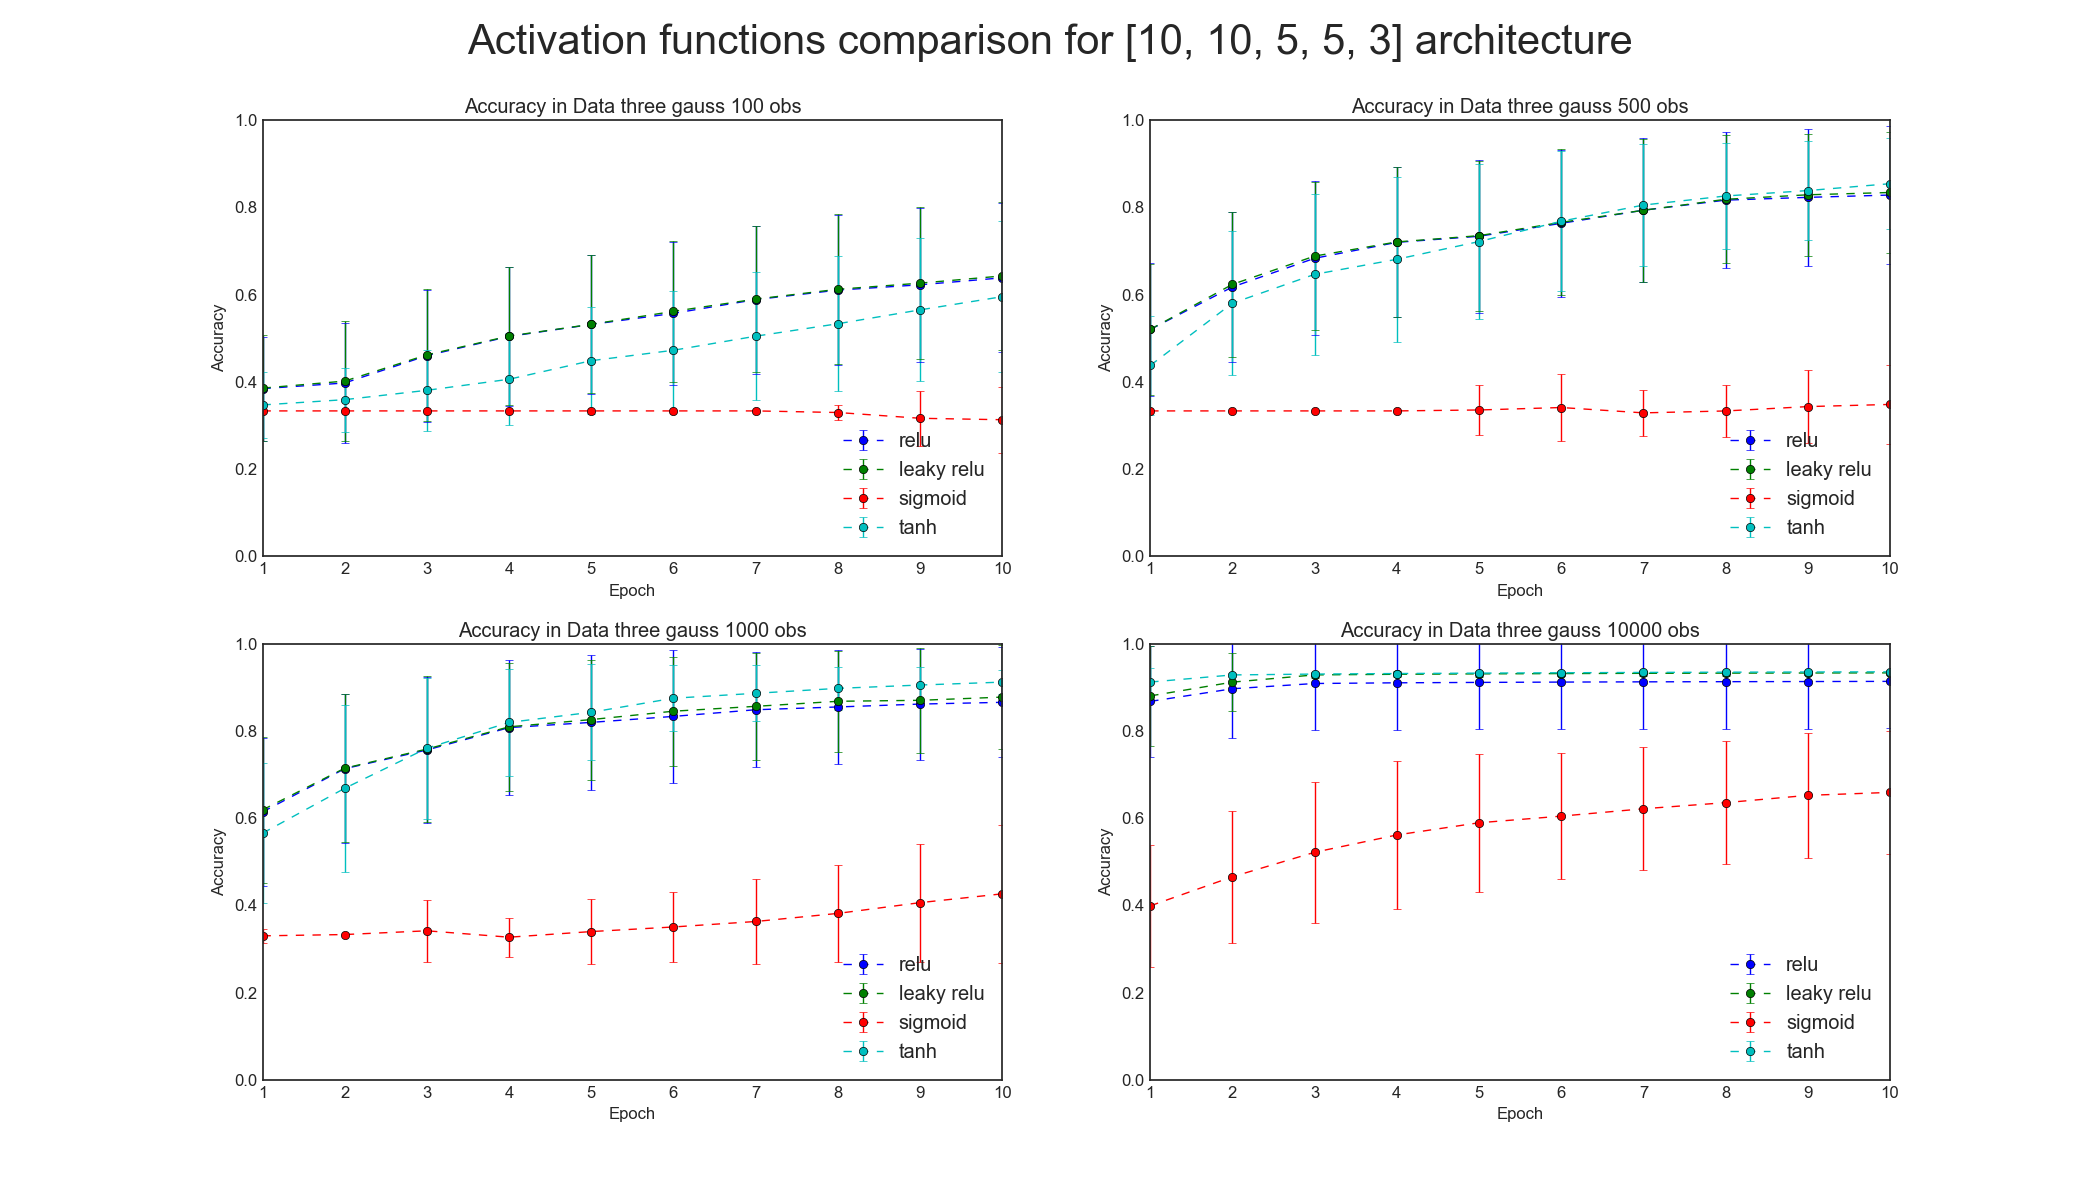
\includegraphics[width=1.4\textwidth]{results/classification/architecture-6/activation_function_data_gauss_2020_03_24_11_31_45.png}}
\end{figure}


\centerline{
\begin{tabular}{lllll}
\hline
{} &          relu &    leaky relu &       sigmoid &          tanh \\
\hline
Data three gauss 100 obs   &  0.64 +- 0.17 &  0.64 +- 0.17 &  0.33 +- 0.00 &  0.60 +- 0.17 \\
Data three gauss 500 obs   &  0.83 +- 0.16 &  0.83 +- 0.14 &  0.35 +- 0.09 &  0.85 +- 0.10 \\
Data three gauss 1000 obs  &  0.87 +- 0.13 &  0.88 +- 0.12 &  0.43 +- 0.16 &  0.91 +- 0.03 \\
Data three gauss 10000 obs &  0.91 +- 0.11 &  0.93 +- 0.01 &  0.66 +- 0.14 &  0.94 +- 0.00 \\
\hline
\end{tabular}
}

\newpage
% ----------------- INERTIA ACTIVATION DATA  -------------------------
\begin{figure}[!ht]
    \noindent\makebox[\textwidth]{%
   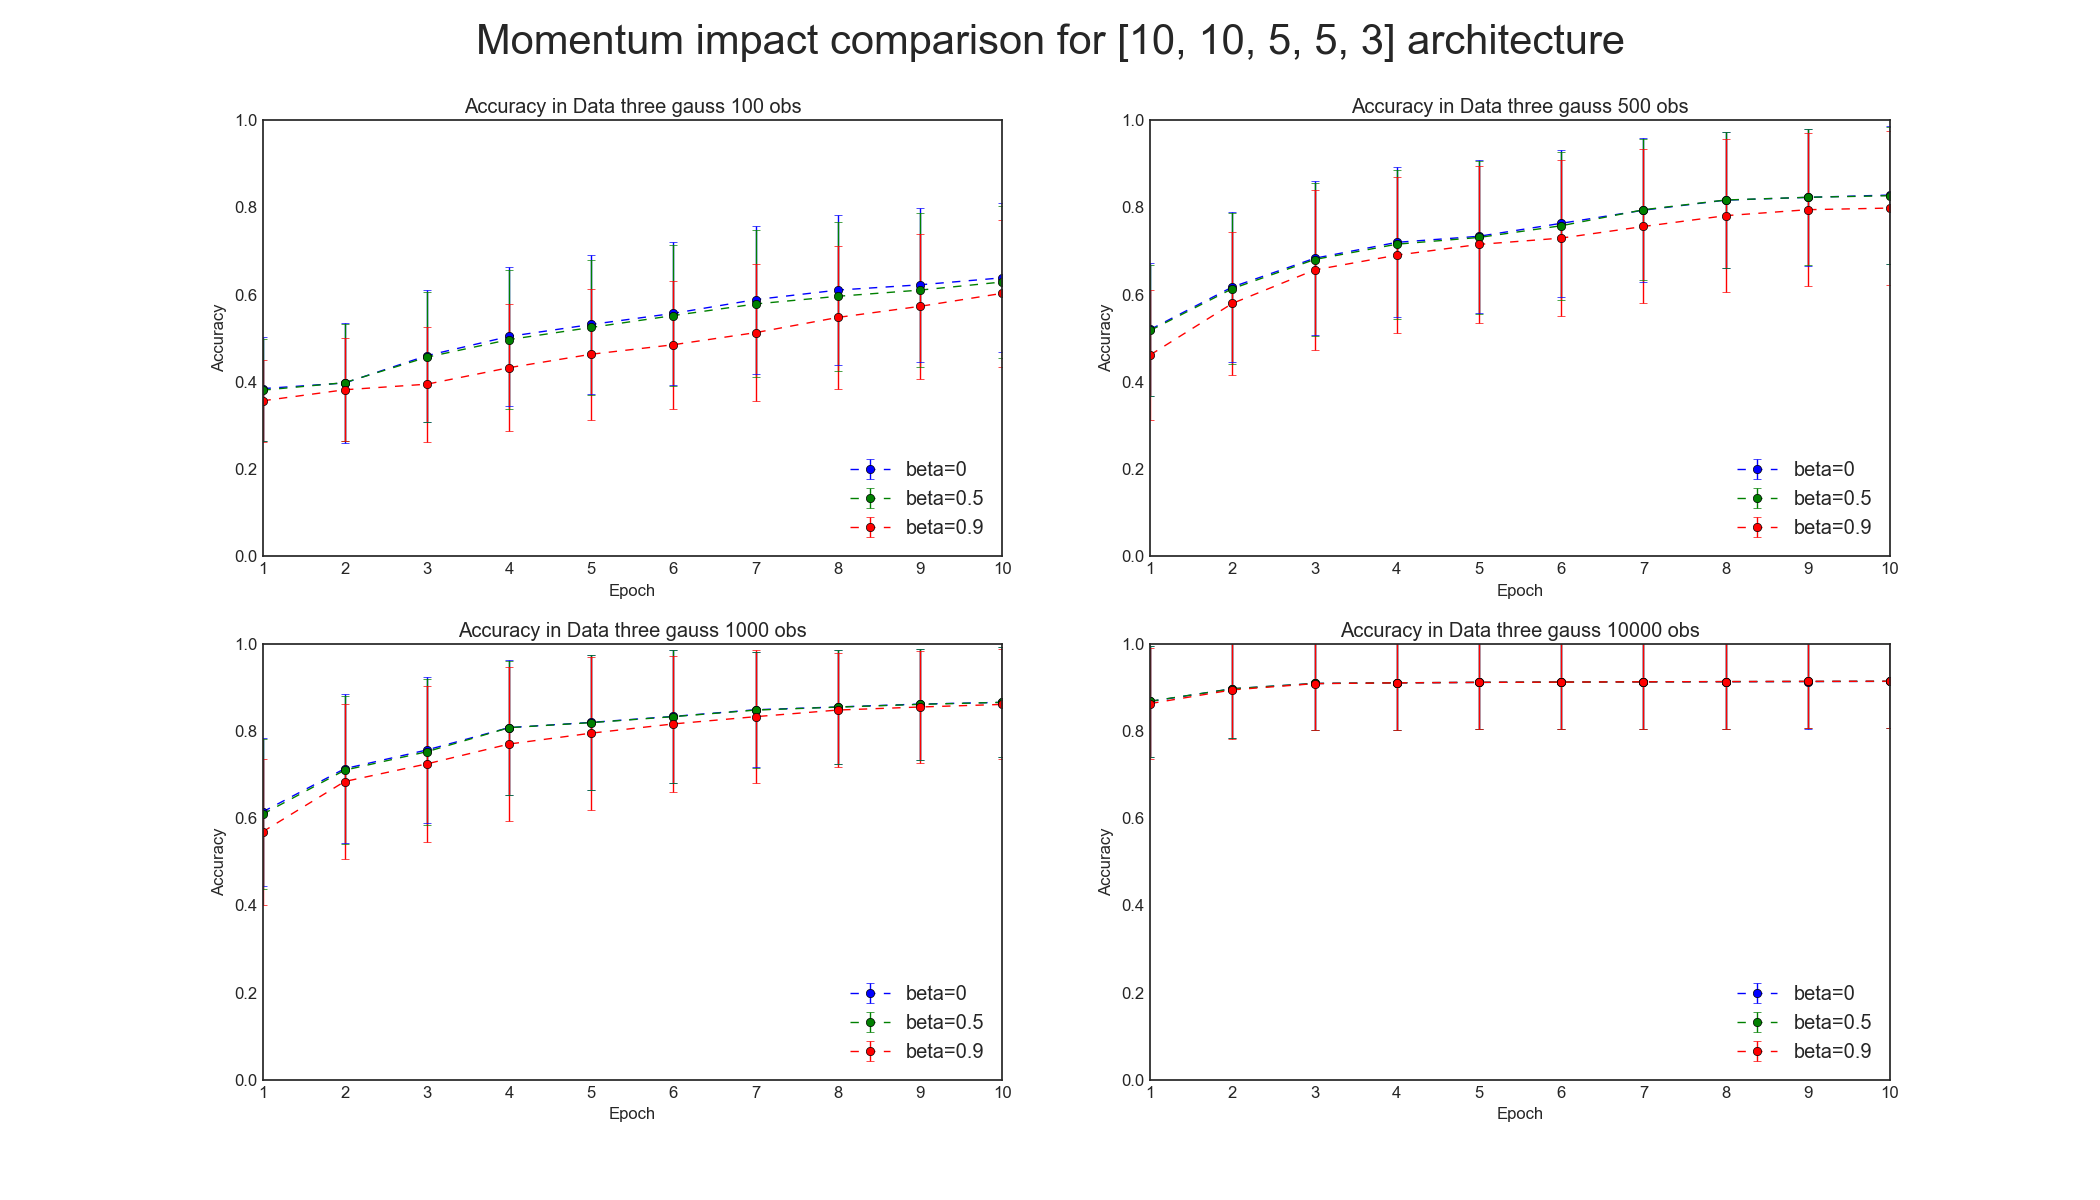
\includegraphics[width=1.4\textwidth]{results/classification/architecture-6/inertia_data_gauss_2020_03_24_11_31_46.png}}
\end{figure}


\centerline{
\begin{tabular}{llll}
\hline
{} &        beta=0 &      beta=0.5 &      beta=0.9 \\
\hline
Data three gauss 100 obs   &  0.64 +- 0.17 &  0.63 +- 0.17 &  0.60 +- 0.17 \\
Data three gauss 500 obs   &  0.83 +- 0.16 &  0.83 +- 0.16 &  0.80 +- 0.18 \\
Data three gauss 1000 obs  &  0.87 +- 0.13 &  0.87 +- 0.13 &  0.86 +- 0.13 \\
Data three gauss 10000 obs &  0.91 +- 0.11 &  0.91 +- 0.11 &  0.91 +- 0.11 \\
\hline
\end{tabular}
}

\newpage
% ----------------- BS ACTIVATION DATA  -------------------------
\begin{figure}[!ht]
    \noindent\makebox[\textwidth]{%
   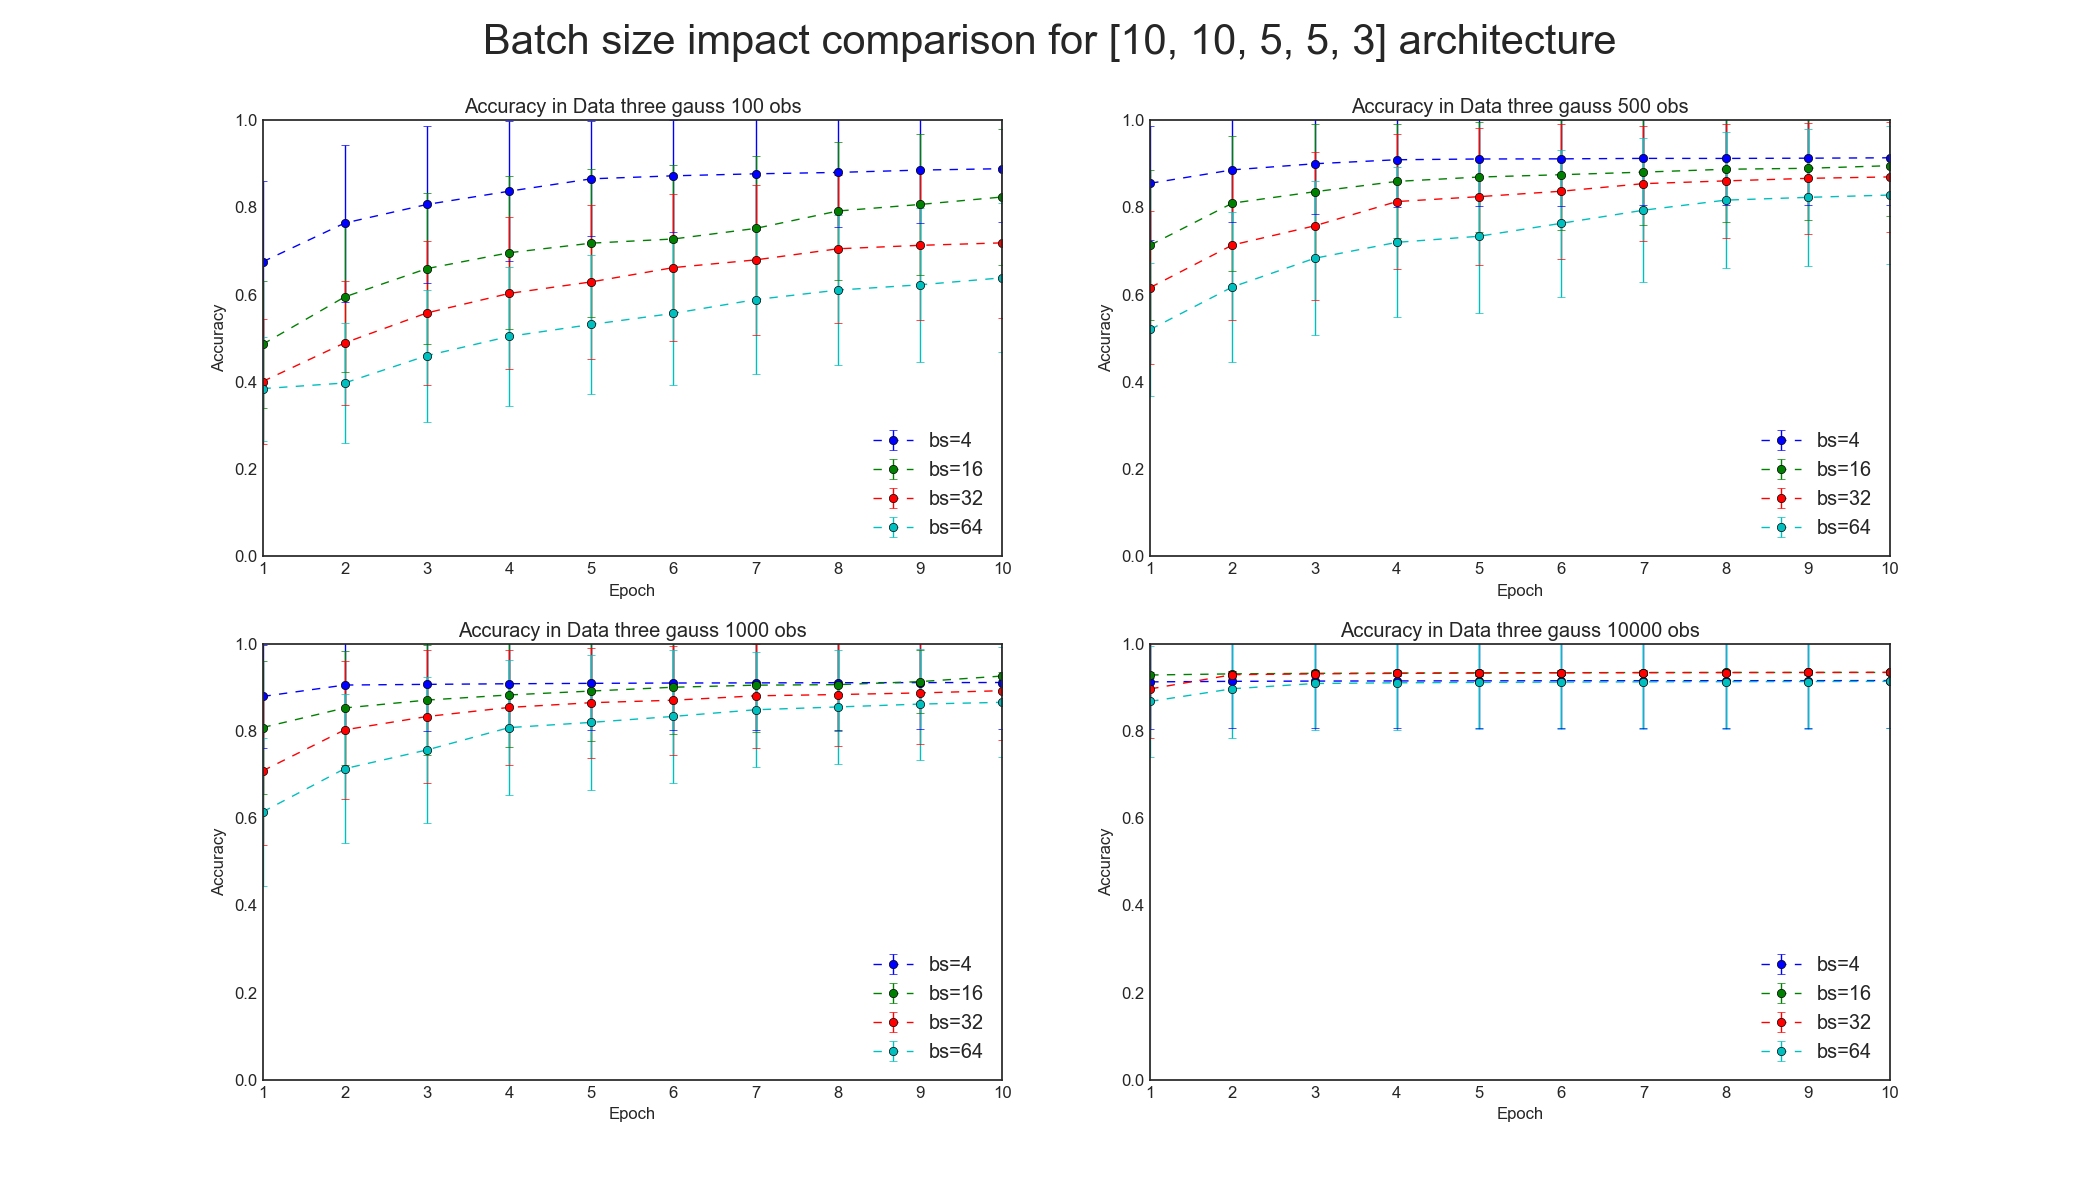
\includegraphics[width=1.4\textwidth]{results/classification/architecture-6/batch_size_data_gauss_2020_03_24_11_31_46.png}}
\end{figure}

\centerline{
\begin{tabular}{lllll}
\hline
{} &          bs=4 &         bs=16 &         bs=32 &         bs=64 \\
\hline
Data three gauss 100 obs   &  0.89 +- 0.12 &  0.82 +- 0.16 &  0.72 +- 0.17 &  0.64 +- 0.17 \\
Data three gauss 500 obs   &  0.91 +- 0.11 &  0.90 +- 0.11 &  0.87 +- 0.13 &  0.83 +- 0.16 \\
Data three gauss 1000 obs  &  0.91 +- 0.11 &  0.93 +- 0.01 &  0.89 +- 0.11 &  0.87 +- 0.13 \\
Data three gauss 10000 obs &  0.92 +- 0.11 &  0.93 +- 0.01 &  0.93 +- 0.01 &  0.91 +- 0.11 \\
\hline
\end{tabular}
}


\newpage
\subsubsection{Conclusion}
Similarly to Simple dataset, in Three Gauss dataset we've had no problems with exploding gradient during learning process. Learning rate and activation function experiment results were similar to those in Simple dataset. Momentum had a slightly bigger impact, especially in more complicated network architectures. Again, smaller batch size resulted in better learning accuracy (after fixed number of epochs).







\newpage
\section{Testing on regression datasets}
In all experiments we are using a ``default'' neural network with parameters:
\begin{itemize}
    \item \texttt{neuron\_numbers}: depending on architecture
    \item \texttt{activation\_functions}: depending on architecture,
    \item \texttt{loss\_function}: 'mean\_squared\_error',
    \item \texttt{batch\_size}: 64,
    \item \texttt{num\_epochs}: 10,
    \item \texttt{output\_activation}: 'linear'
    \item \texttt{learning\_rate}: 0.001.
\end{itemize}
In each experiments we are testing influence of changing one of the parameter on accuracy of the test set. Each experiment is repeated 30 times, and mean accuracy is displayed on the graph along with standard deviation. 

Parameters tested in experiments are presented in table below. 

\bgroup
\def\arraystretch{1.5}
\begin{table}[!h]
    \centering
    \begin{tabular}{ll}
        Parameter              & Tested values \\ \hline
        Learning rate $\alpha$ &    0.01, 0.001, 0.0001, 0.00001           \\
        Momentum $\beta$       &    0, 0.5, 0.9           \\
        Batch size             &    4, 16, 32, 64       
    \end{tabular}
    \caption{Parameters tested in experiments.}
\end{table}
\egroup

Since our empirical test showed, that activation function combination is much more important in regression than in classification problems, we decided that activation function will be now tested as part of architecture (instead of parameter, like in classification task). 

\newpage
\subsection{Activation}

\subsubsection{Architecture 1}
\[[]\]
No hidden layers. 


% ----------------- LR ACTIVATION DATA  -------------------------

\begin{figure}[!ht]
    \noindent\makebox[\textwidth]{%
   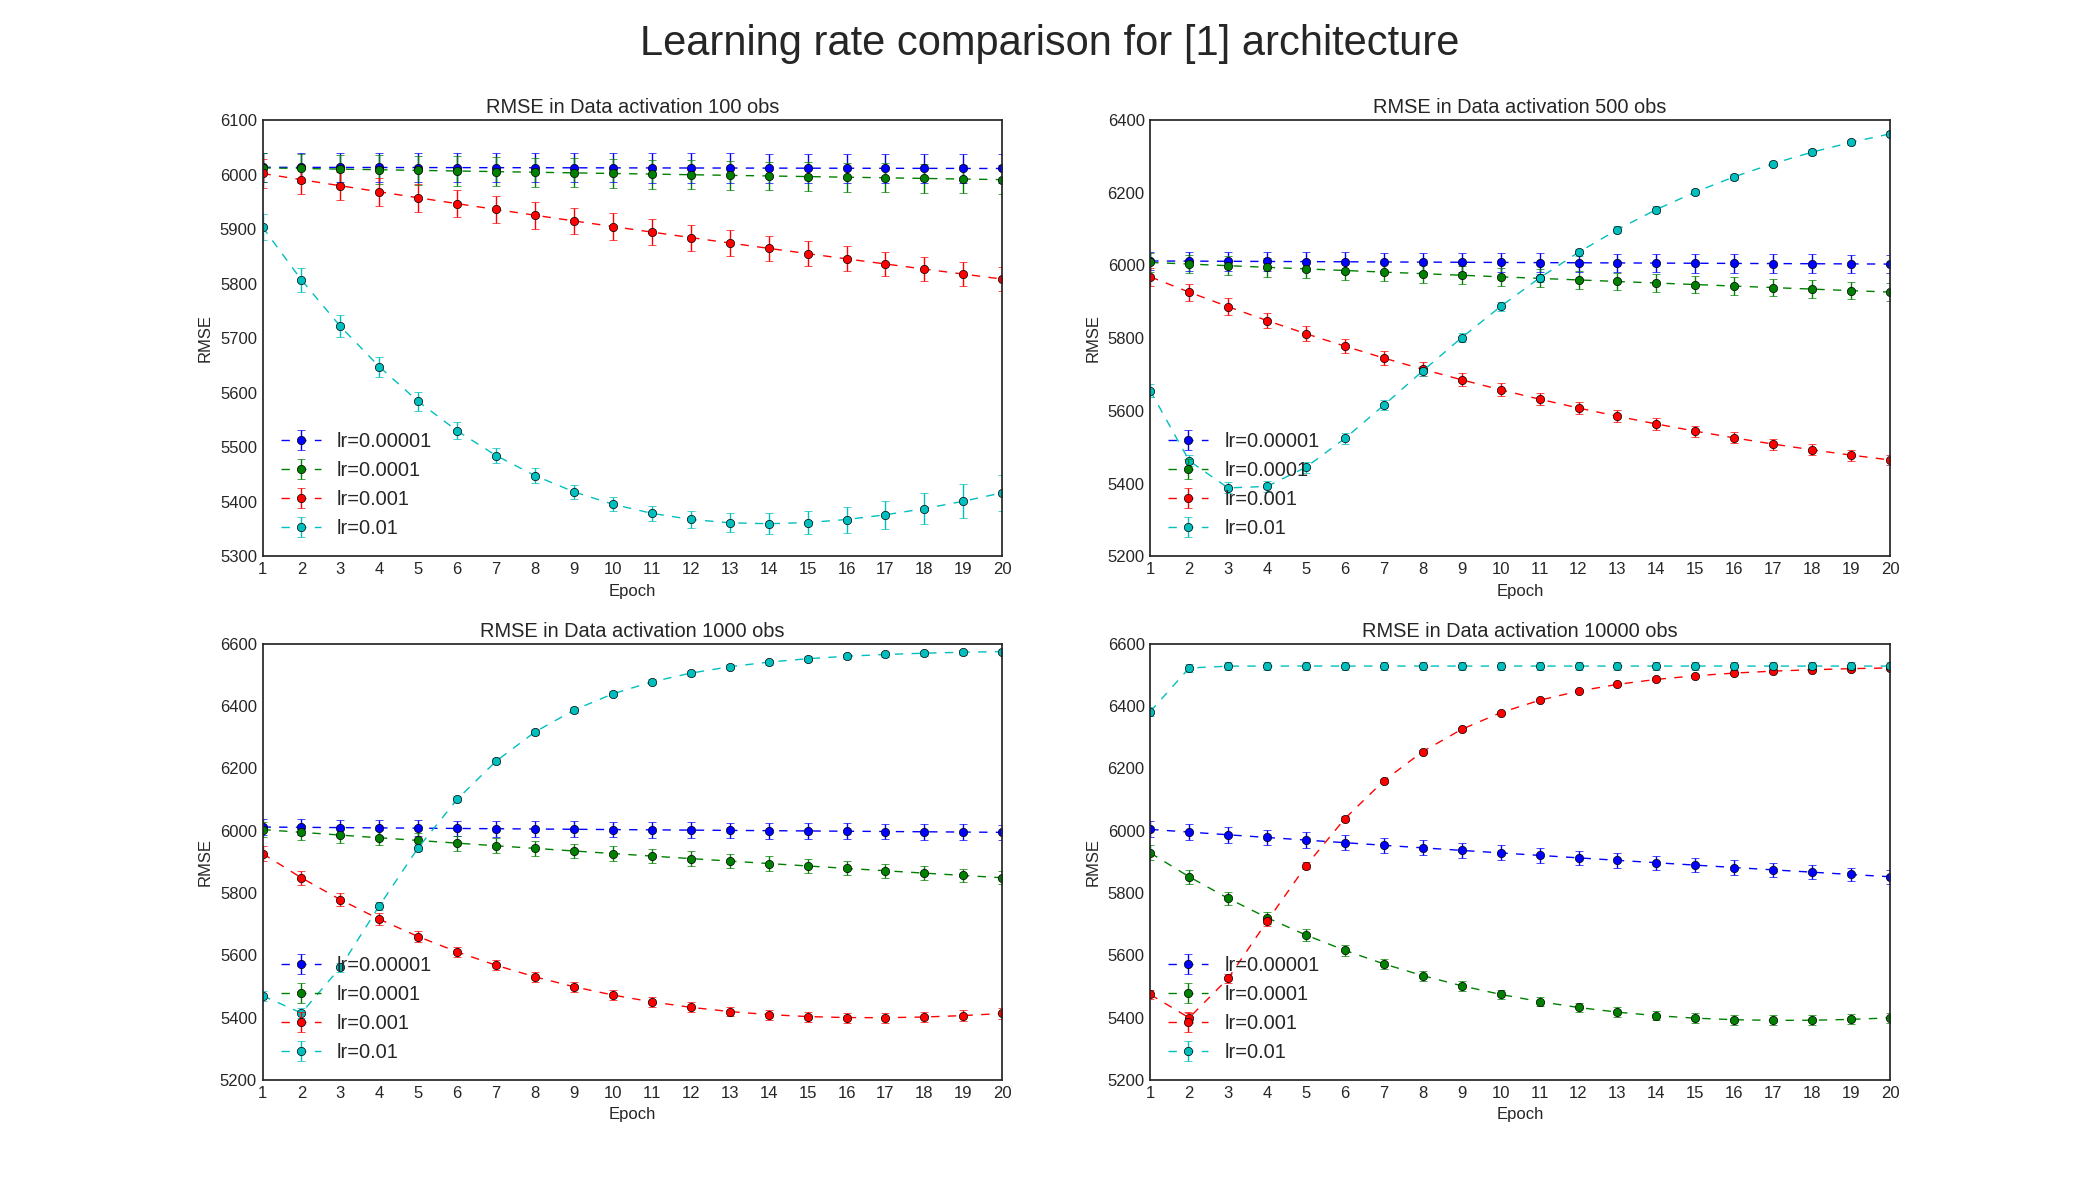
\includegraphics[width=1.4\textwidth]{results/regression/architecture-1/lr_data_activation_2020_03_24_03_12_00.png}}
\end{figure}

\centerline{
    \begin{tabular}{|l|llll|}
    \hline 
    {} &        lr=0.00001 &         lr=0.0001 &          lr=0.001 &           lr=0.01 \\
\hline
Data activation 100 obs   &  6011.09 +- 26.76 &  5990.64 +- 26.26 &  5808.39 +- 22.12 &  5359.81 +- 19.24 \\
Data activation 500 obs   &  6003.82 +- 25.71 &  5926.72 +- 23.72 &  5465.09 +- 14.83 &  5388.21 +- 15.22 \\
Data activation 1000 obs  &  5994.61 +- 25.04 &  5848.79 +- 21.50 &  5399.91 +- 16.18 &  5414.86 +- 16.42 \\
Data activation 10000 obs &  5852.03 +- 22.04 &  5391.29 +- 15.70 &  5399.41 +- 16.07 &  6382.07 +- 13.50 \\
\hline
\end{tabular}
}

\newpage
% ----------------- INERTIA ACTIVATION DATA  -------------------------
\begin{figure}[!ht]
    \noindent\makebox[\textwidth]{%
   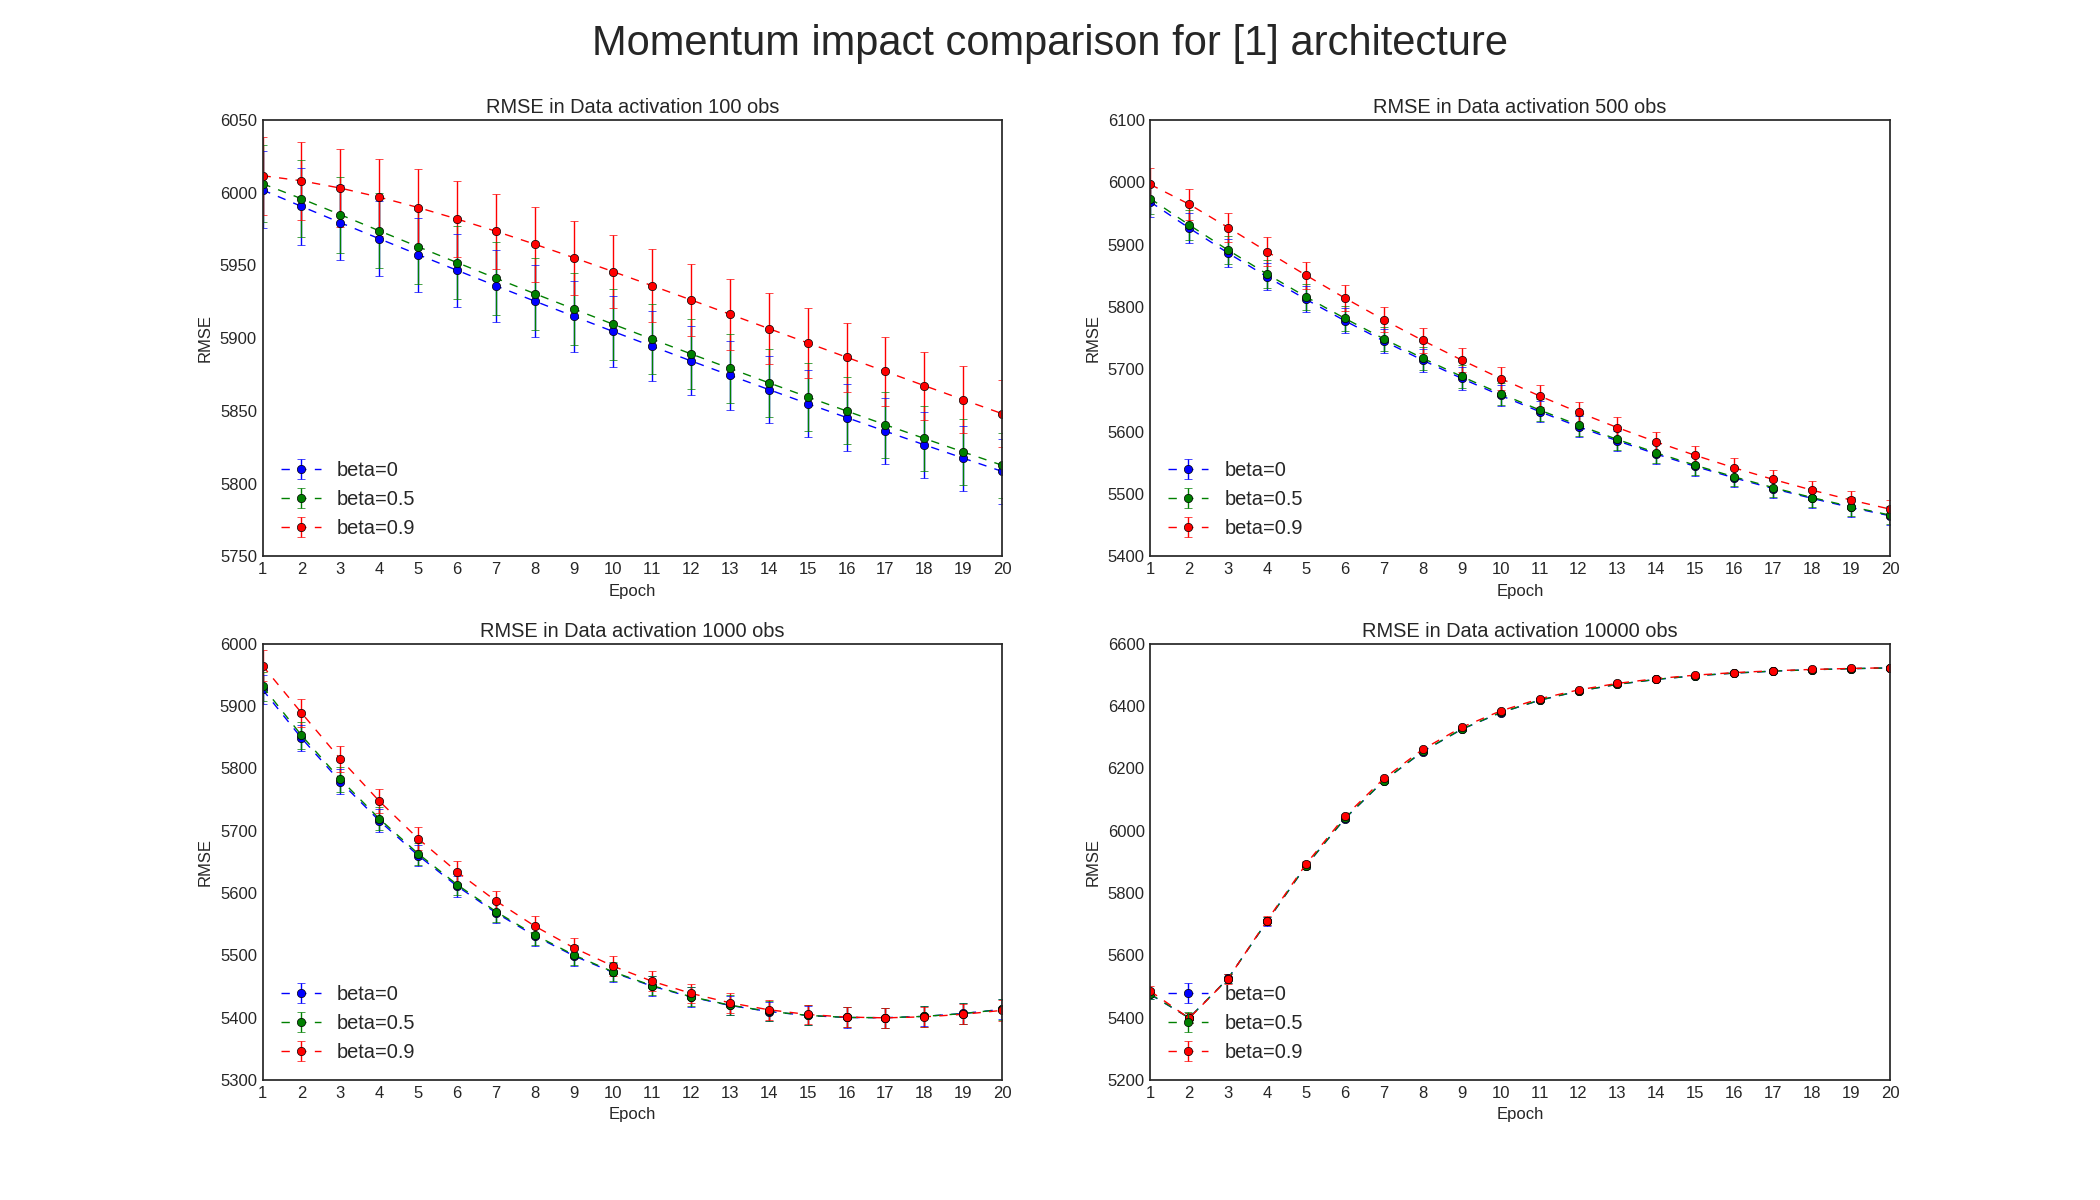
\includegraphics[width=1.4\textwidth]{results/regression/architecture-1/inertia_data_activation_2020_03_24_03_12_00.png}}
\end{figure}




\centerline{
\begin{tabular}{|l|lll|}
\hline
{} &            beta=0 &          beta=0.5 &          beta=0.9 \\
\hline
Data activation 100 obs   &  5808.39 +- 22.12 &  5812.60 +- 22.17 &  5848.07 +- 22.95 \\
Data activation 500 obs   &  5465.09 +- 14.83 &  5466.18 +- 14.85 &  5475.75 +- 14.88 \\
Data activation 1000 obs  &  5399.91 +- 16.18 &  5399.91 +- 16.17 &  5399.73 +- 16.12 \\
Data activation 10000 obs &  5399.41 +- 16.07 &  5399.20 +- 16.04 &  5398.03 +- 15.92 \\
\hline
\end{tabular}
}

\newpage
% ----------------- BS ACTIVATION DATA  -------------------------
\begin{figure}[!ht]
    \noindent\makebox[\textwidth]{%
   \includegraphics[width=1.4\textwidth]{results/regression/architecture-1/batch_size_data_activation_2020_03_24_03_12_01.png}}
\end{figure}

\centerline{
\begin{tabular}{|l|llll|}
\hline
{} &              bs=4 &             bs=16 &             bs=32 &             bs=64 \\
\hline
Data activation 100 obs   &  5357.69 +- 14.37 &  5488.17 +- 19.96 &  5654.60 +- 31.88 &  5808.39 +- 22.12 \\
Data activation 500 obs   &  5385.71 +- 15.27 &  5382.06 +- 15.53 &  5381.95 +- 16.06 &  5465.09 +- 14.83 \\
Data activation 1000 obs  &  5401.61 +- 15.77 &  5401.00 +- 16.08 &  5401.23 +- 16.44 &  5399.91 +- 16.18 \\
Data activation 10000 obs &  6501.88 +- 16.35 &  5705.04 +- 13.58 &  5398.56 +- 15.86 &  5399.41 +- 16.07 \\
\hline
\end{tabular}}

\newpage
\subsubsection{Architecture 2}
\[[5]\]
One hidden layer with 5 neurons and \texttt{tanh} activation function.

% ----------------- LR ACTIVATION DATA  -------------------------
\begin{figure}[!ht]
    \noindent\makebox[\textwidth]{%
   \includegraphics[width=1.4\textwidth]{results/regression/architecture-2/lr_data_activation_2020_03_24_03_33_33.png}}
\end{figure}

\centerline{
\begin{tabular}{|l|llll|}
\hline
{} &        lr=0.00001 &         lr=0.0001 &          lr=0.001 &           lr=0.01 \\
\hline
Data activation 100 obs   &   5983.99 +- 62.44 &  5732.90 +- 176.85 &  5332.89 +- 234.81 &  7104.08 +- 2190.67 \\
Data activation 500 obs   &   5920.93 +- 81.26 &  5281.19 +- 217.04 &  5350.26 +- 266.70 &          nan +- nan \\
Data activation 1000 obs  &  5804.73 +- 137.02 &  5303.54 +- 237.34 &  6086.08 +- 272.34 &          nan +- nan \\
Data activation 10000 obs &  5293.77 +- 208.54 &  6014.91 +- 253.48 &   6720.89 +- 30.26 &          nan +- nan \\
\hline
\end{tabular}}

\newpage
% ----------------- INERTIA ACTIVATION DATA  -------------------------
\begin{figure}[!ht]
    \noindent\makebox[\textwidth]{%
   \includegraphics[width=1.4\textwidth]{results/regression/architecture-2/inertia_data_activation_2020_03_24_03_33_34.png}}
\end{figure}

\centerline{
\begin{tabular}{|l|lll|}
\hline 
{} &            beta=0 &          beta=0.5 &          beta=0.9 \\
\hline
Data activation 100 obs   &  5332.89 +- 234.81 &  5342.46 +- 259.90 &  5359.03 +- 267.01 \\
Data activation 500 obs   &  5350.26 +- 266.70 &  5496.95 +- 266.97 &  5433.66 +- 280.52 \\
Data activation 1000 obs  &  6086.08 +- 272.34 &  6009.20 +- 489.68 &  5429.91 +- 280.96 \\
Data activation 10000 obs &   6720.89 +- 30.26 &   6718.34 +- 24.63 &   6718.77 +- 26.14 \\
\hline
\end{tabular}}

\newpage
% ----------------- BS ACTIVATION DATA  -------------------------
\begin{figure}[!ht]
    \noindent\makebox[\textwidth]{%
   \includegraphics[width=1.4\textwidth]{results/regression/architecture-2/batch_size_data_activation_2020_03_24_03_33_35.png}}
\end{figure}

\centerline{
\begin{tabular}{|l|llll|}
\hline
{} &              bs=4 &             bs=16 &             bs=32 &             bs=64 \\
\hline
Data activation 100 obs   &  6303.20 +- 167.11 &  5451.32 +- 275.05 &  5375.17 +- 253.04 &  5332.89 +- 234.81 \\
Data activation 500 obs   &   6668.57 +- 64.87 &  6387.09 +- 283.43 &  6012.97 +- 305.86 &  5350.26 +- 266.70 \\
Data activation 1000 obs  &   6751.67 +- 72.19 &   6663.50 +- 65.17 &  6455.68 +- 274.11 &  6086.08 +- 272.34 \\
Data activation 10000 obs &  6730.88 +- 194.59 &   6775.66 +- 45.66 &   6743.45 +- 51.77 &   6720.89 +- 30.26 \\
\hline 
\end{tabular}}


\newpage
\subsubsection{Architecture 3}
\[[5, 5]\]
Two hidden layers with 5 neurons each, $[\texttt{tanh}, \texttt{linear}]$ activation functions.

% ----------------- LR ACTIVATION DATA  -------------------------
\begin{figure}[!ht]
    \noindent\makebox[\textwidth]{%
   \includegraphics[width=1.4\textwidth]{results/regression/architecture-3/lr_data_activation_2020_03_24_03_58_53.png}}
\end{figure}


\centerline{
\begin{tabular}{|l|llll|}
\hline
{} &        lr=0.00001 &         lr=0.0001 &          lr=0.001 &           lr=0.01 \\
\hline
Data activation 100 obs   &   5989.44 +- 44.84 &  5535.86 +- 421.40 &  5639.58 +- 790.70 &               253360.62 +- 308602.59 \\
Data activation 500 obs   &  5826.83 +- 170.57 &  5599.17 +- 455.75 &  5411.55 +- 454.91 &            2884109.96 +- 14720152.73 \\
Data activation 1000 obs  &  5524.36 +- 442.25 &  5643.51 +- 466.91 &  5516.16 +- 494.07 &  268587542066.87 +- 1433085108303.57 \\
Data activation 10000 obs &  5598.23 +- 448.36 &  6558.38 +- 321.73 &  5383.36 +- 552.76 &                      4332.07 +- 9.49 \\
\hline
\end{tabular}}

\newpage
% ----------------- INERTIA ACTIVATION DATA  -------------------------
\begin{figure}[!ht]
    \noindent\makebox[\textwidth]{%
   \includegraphics[width=1.4\textwidth]{results/regression/architecture-3/inertia_data_activation_2020_03_24_03_58_54.png}}
\end{figure}


\centerline{
\begin{tabular}{|l|lll|}
\hline 
{} &            beta=0 &          beta=0.5 &          beta=0.9 \\
\hline
Data activation 100 obs   &  5639.58 +- 790.70 &   5663.01 +- 281.83 &  5595.67 +- 643.14 \\
Data activation 500 obs   &  5411.55 +- 454.91 &  6224.53 +- 1189.41 &  5727.13 +- 228.64 \\
Data activation 1000 obs  &  5516.16 +- 494.07 &   6558.11 +- 578.34 &  6523.97 +- 850.98 \\
Data activation 10000 obs &  5383.36 +- 552.76 &   6656.16 +- 314.49 &  6698.74 +- 301.72 \\
\hline
\end{tabular}}

\newpage
% ----------------- BS ACTIVATION DATA  -------------------------
\begin{figure}[!ht]
    \noindent\makebox[\textwidth]{%
   \includegraphics[width=1.4\textwidth]{results/regression/architecture-3/batch_size_data_activation_2020_03_24_03_58_54.png}}
\end{figure}


\centerline{
\begin{tabular}{|l|llll|}
\hline
{} &              bs=4 &             bs=16 &             bs=32 &             bs=64 \\
\hline
Data activation 100 obs   &  5088.57 +- 255.78 &  5345.65 +- 395.72 &  5409.40 +- 459.54 &  5639.58 +- 790.70 \\
Data activation 500 obs   &  4791.65 +- 422.23 &  5235.80 +- 338.63 &  5434.64 +- 558.29 &  5411.55 +- 454.91 \\
Data activation 1000 obs  &  4694.47 +- 394.48 &  5263.16 +- 405.86 &  5277.10 +- 469.62 &  5516.16 +- 494.07 \\
Data activation 10000 obs &  4503.40 +- 412.34 &  5121.94 +- 606.30 &  5350.60 +- 539.34 &  5383.36 +- 552.76 \\
\hline 
\end{tabular}}


\newpage
\subsubsection{Architecture 4}
\[[5, 5]\]
Two hidden layers with 5 neurons each, $[\texttt{tanh}, \texttt{tanh}]$ activation functions.

% ----------------- LR ACTIVATION DATA  -------------------------
\begin{figure}[!ht]
    \noindent\makebox[\textwidth]{%
   \includegraphics[width=1.4\textwidth]{results/regression/architecture-4/lr_data_activation_2020_03_24_04_24_10.png}}
\end{figure}


\centerline{
\begin{tabular}{|l|llll|}
\hline
{} &        lr=0.00001 &         lr=0.0001 &          lr=0.001 &           lr=0.01 \\
\hline
Data activation 100 obs   &   5989.44 +- 44.84 &  5535.86 +- 421.40 &  5639.58 +- 790.70 &               253360.62 +- 308602.59 \\
Data activation 500 obs   &  5826.83 +- 170.57 &  5599.17 +- 455.75 &  5411.55 +- 454.91 &            2884109.96 +- 14720152.73 \\
Data activation 1000 obs  &  5524.36 +- 442.25 &  5643.51 +- 466.91 &  5516.16 +- 494.07 &  268587542066.87 +- 1433085108303.57 \\
Data activation 10000 obs &  5598.23 +- 448.36 &  6558.38 +- 321.73 &  5383.36 +- 552.76 &                      4332.07 +- 9.49 \\
\hline
\end{tabular}}

\newpage
% ----------------- INERTIA ACTIVATION DATA  -------------------------
\begin{figure}[!ht]
    \noindent\makebox[\textwidth]{%
   \includegraphics[width=1.4\textwidth]{results/regression/architecture-4/inertia_data_activation_2020_03_24_04_24_10.png}}
\end{figure}


\centerline{
\begin{tabular}{|l|lll|}
\hline 
{} &            beta=0 &          beta=0.5 &          beta=0.9 \\
\hline
Data activation 100 obs   &  5639.58 +- 790.70 &   5663.01 +- 281.83 &  5595.67 +- 643.14 \\
Data activation 500 obs   &  5411.55 +- 454.91 &  6224.53 +- 1189.41 &  5727.13 +- 228.64 \\
Data activation 1000 obs  &  5516.16 +- 494.07 &   6558.11 +- 578.34 &  6523.97 +- 850.98 \\
Data activation 10000 obs &  5383.36 +- 552.76 &   6656.16 +- 314.49 &  6698.74 +- 301.72 \\
\hline
\end{tabular}}

\newpage
% ----------------- BS ACTIVATION DATA  -------------------------
\begin{figure}[!ht]
    \noindent\makebox[\textwidth]{%
   \includegraphics[width=1.4\textwidth]{results/regression/architecture-4/batch_size_data_activation_2020_03_24_04_24_11.png}}
\end{figure}


\centerline{
\begin{tabular}{|l|llll|}
\hline
{} &              bs=4 &             bs=16 &             bs=32 &             bs=64 \\
\hline
Data activation 100 obs   &  5088.57 +- 255.78 &  5345.65 +- 395.72 &  5409.40 +- 459.54 &  5639.58 +- 790.70 \\
Data activation 500 obs   &  4791.65 +- 422.23 &  5235.80 +- 338.63 &  5434.64 +- 558.29 &  5411.55 +- 454.91 \\
Data activation 1000 obs  &  4694.47 +- 394.48 &  5263.16 +- 405.86 &  5277.10 +- 469.62 &  5516.16 +- 494.07 \\
Data activation 10000 obs &  4503.40 +- 412.34 &  5121.94 +- 606.30 &  5350.60 +- 539.34 &  5383.36 +- 552.76 \\
\hline 
\end{tabular}}

\newpage
\subsubsection{Architecture 5}
\[[5, 5, 5, 5]\]
Four hidden layers with 5 neurons each, $[\texttt{tanh}, \texttt{tanh}, texttt{tanh}, \texttt{tanh}]$ activation functions.
% ----------------- LR ACTIVATION DATA  -------------------------
\begin{figure}[!ht]
    \noindent\makebox[\textwidth]{%
   \includegraphics[width=1.4\textwidth]{results/regression/architecture-5/lr_data_activation_2020_03_24_04_56_25.png}}
\end{figure}



\centerline{
\begin{tabular}{|l|llll|}
\hline
{} &        lr=0.00001 &         lr=0.0001 &          lr=0.001 &           lr=0.01 \\
\hline
Data activation 100 obs   &  5846.75 +- 310.63 &  5873.25 +- 270.74 &                               23628.63 +- 52913.76 &  nan +- nan \\
Data activation 500 obs   &  5818.22 +- 393.04 &  5841.13 +- 424.54 &                          4619004.82 +- 24695226.62 &  nan +- nan \\
Data activation 1000 obs  &  5822.36 +- 402.72 &  6040.81 +- 605.40 &                    9785475766.02 +- 51945187413.74 &  nan +- nan \\
Data activation 10000 obs &  5994.99 +- 367.36 &  6398.52 +- 530.68 &  8e21.00 +- 4e16 &  nan +- nan \\
\hline
\end{tabular}}

\newpage
% ----------------- INERTIA ACTIVATION DATA  -------------------------
\begin{figure}[!ht]
    \noindent\makebox[\textwidth]{%
   \includegraphics[width=1.4\textwidth]{results/regression/architecture-5/inertia_data_activation_2020_03_24_04_56_26.png}}
\end{figure}


\centerline{
\begin{tabular}{|l|lll|}
\hline 
{} &            beta=0 &          beta=0.5 &          beta=0.9 \\
\hline
Data activation 100 obs   &                               23628.63 +- 52913.76 &    5378.28 +- 646.00 &  5368.43 +- 570.03 \\
Data activation 500 obs   &                          4619004.82 +- 24695226.62 &    5205.86 +- 520.61 &  5241.32 +- 631.35 \\
Data activation 1000 obs  &                    9785475766.02 +- 51945187413.74 &  9196.12 +- 16485.11 &  5185.46 +- 508.40 \\
Data activation 10000 obs &  8e22.00 +- 43583919932154918... &    4438.96 +- 243.61 &  4859.72 +- 696.73 \\
\hline
\end{tabular}}

\newpage
% ----------------- BS ACTIVATION DATA  -------------------------
\begin{figure}[!ht]
    \noindent\makebox[\textwidth]{%
   \includegraphics[width=1.4\textwidth]{results/regression/architecture-5/batch_size_data_activation_2020_03_24_04_56_26.png}}
\end{figure}


\centerline{
\begin{tabular}{|l|llll|}
\hline
{} &              bs=4 &             bs=16 &             bs=32 &             bs=64 \\
\hline
Data activation 100 obs   &                      3e8 +- 1.8e9 &                      232362.17 +- 1179235.42 &         1e6 +- 4.6e6 &                               23628.63 +- 52913.76 \\
Data activation 500 obs   &                                  4366.57 +- 112.70 &  2.9e14.00 +- 1.5e16.00 &  3e12 +- 1.6e10 &                          4619004.82 +- 2e7 \\
Data activation 1000 obs  &  1e37.00 +- 73... &                        26112.91 +- 116771.34 &            8e4 +- 404360.55 &                    9785475766.02 +- 5e10 \\
Data activation 10000 obs &  6e38.00 +- ... &                             4340.35 +- 73.05 &          4e5 +- 2185766.81 &  8e21.00 +- 4e16... \\
\hline 
\end{tabular}}

\newpage
\subsubsection{Architecture 6}
\[[5, 5, 5, 5]\]
Four hidden layers with 5 neurons each, $[\texttt{relu}, \texttt{tanh}, \texttt{tanh}, \texttt{linear}]$ activation functions.

% ----------------- LR ACTIVATION DATA  -------------------------
\begin{figure}[!ht]
    \noindent\makebox[\textwidth]{%
   \includegraphics[width=1.4\textwidth]{results/regression/architecture-6/lr_data_activation_2020_03_24_05_28_31.png}}
\end{figure}


\centerline{
\begin{tabular}{|l|llll|}
\hline
{} &        lr=0.00001 &         lr=0.0001 &          lr=0.001 &           lr=0.01 \\
\hline
Data activation 100 obs   &  5846.75 +- 310.63 &  5873.25 +- 270.74 &                               23628.63 +- 52913.76 &  nan +- nan \\
Data activation 500 obs   &  5818.22 +- 393.04 &  5841.13 +- 424.54 &                          4619004.82 +- 24695226.62 &  nan +- nan \\
Data activation 1000 obs  &  5822.36 +- 402.72 &  6040.81 +- 605.40 &                    9785475766.02 +- 51945187413.74 &  nan +- nan \\
Data activation 10000 obs &  5994.99 +- 367.36 &  6398.52 +- 530.68 &  8e21 +- 4e16 &  nan +- nan \\
\hline
\end{tabular}}

\newpage
% ----------------- INERTIA ACTIVATION DATA  -------------------------

\begin{figure}[!ht]
    \noindent\makebox[\textwidth]{%
   \includegraphics[width=1.4\textwidth]{results/regression/architecture-6/inertia_data_activation_2020_03_24_05_28_32.png}}
\end{figure}


\centerline{
\begin{tabular}{|l|lll|}
\hline 
{} &            beta=0 &          beta=0.5 &          beta=0.9 \\
\hline
Data activation 100 obs   &                               23628.63 +- 52913.76 &    5378.28 +- 646.00 &  5368.43 +- 570.03 \\
Data activation 500 obs   &                          4619004.82 +- 24695226.62 &    5205.86 +- 520.61 &  5241.32 +- 631.35 \\
Data activation 1000 obs  &                    9785475766.02 +- 51945187413.74 &  9196.12 +- 16485.11 &  5185.46 +- 508.40 \\
Data activation 10000 obs &  8093330750883057631232.00 +- 43583919932154918... &    4438.96 +- 243.61 &  4859.72 +- 696.73 \\
\hline
\end{tabular}}

\newpage
% ----------------- BS ACTIVATION DATA  -------------------------
\begin{figure}[!ht]
    \noindent\makebox[\textwidth]{%
   \includegraphics[width=1.4\textwidth]{results/regression/architecture-6/batch_size_data_activation_2020_03_24_05_28_33.png}}
\end{figure}


\centerline{
\begin{tabular}{|l|llll|}
\hline
{} &              bs=4 &             bs=16 &             bs=32 &             bs=64 \\
\hline
Data activation 100 obs   &                      3e9 +- 1e8 &                      232362.17 +- 1179235.42 &         1021183.80 +- 4627293.46 &                               23628.63 +- 52913.76 \\
Data activation 500 obs   &                                  4366.57 +- 112.70 &  2.9e15 +- 1e16 &  3e9 +- 1.6e10 &                          4619004.82 +- 24695226.62 \\
Data activation 1000 obs  &  1e36 +- 7e22 &                        26112.91 +- 116771.34 &            81247.69 +- 404360.55 &                    9e9 +- 51945187413.74 \\
Data activation 10000 obs &  6e38 +- 4e23 &                             4340.35 +- 73.05 &          410239.39 +- 2185766.81 &  8e21 +- 4e19 \\
\hline 
\end{tabular}}


\newpage
\subsection{Cube}

\subsubsection{Architecture 1}
\[[]\]
No hidden layers. 

% ----------------- LR CUBE DATA  -------------------------
\begin{figure}[!ht]
    \noindent\makebox[\textwidth]{%
   \includegraphics[width=1.4\textwidth]{results/regression/architecture-1/lr_data_cube_2020_03_24_05_41_36.png}}
\end{figure}


\centerline{
\begin{tabular}{|l|llll|}
\hline
{} &         lr=0.00001 &          lr=0.0001 &           lr=0.001 &           lr=0.01 \\
\hline
Data cube 100 obs   &  12819.09 +- 12.13 &  12816.80 +- 12.02 &  12796.18 +- 11.08 &  12728.48 +- 7.41 \\
Data cube 500 obs   &  12818.35 +- 12.32 &  12808.37 +- 11.66 &   12745.55 +- 7.25 &  12724.06 +- 4.45 \\
Data cube 1000 obs  &  12817.51 +- 12.03 &  12802.18 +- 10.85 &   12741.54 +- 5.09 &  12741.51 +- 5.03 \\
Data cube 10000 obs &  12801.33 +- 10.82 &   12737.81 +- 5.29 &   12737.82 +- 5.30 &  12794.34 +- 2.98 \\
\hline
\end{tabular}}

\newpage
% ----------------- INERTIA CUBE DATA  -------------------------
\begin{figure}[!ht]
    \noindent\makebox[\textwidth]{%
   \includegraphics[width=1.4\textwidth]{results/regression/architecture-1/inertia_data_cube_2020_03_24_05_41_36.png}}
\end{figure}

\centerline{
\begin{tabular}{llll}
\hline
{} &             beta=0 &           beta=0.5 &           beta=0.9 \\
\hline
Data cube 100 obs   &  12796.18 +- 11.08 &  12796.65 +- 11.08 &  12800.68 +- 11.25 \\
Data cube 500 obs   &   12745.55 +- 7.25 &   12745.72 +- 7.26 &   12747.23 +- 7.37 \\
Data cube 1000 obs  &   12741.54 +- 5.09 &   12741.55 +- 5.10 &   12741.66 +- 5.14 \\
Data cube 10000 obs &   12737.82 +- 5.30 &   12737.83 +- 5.28 &   12737.96 +- 5.30 \\
\hline
\end{tabular}}

\newpage
% ----------------- BS CUBE DATA  -------------------------
\begin{figure}[!ht]
    \noindent\makebox[\textwidth]{%
   \includegraphics[width=1.4\textwidth]{results/regression/architecture-1/batch_size_data_cube_2020_03_24_05_41_37.png}}
\end{figure}

\centerline{
\begin{tabular}{lllll}
\hline
{} &              bs=4 &              bs=16 &              bs=32 &              bs=64 \\
\hline
Data cube 100 obs   &  12727.80 +- 4.47 &  12756.25 +- 11.74 &  12778.67 +- 12.91 &  12796.18 +- 11.08 \\
Data cube 500 obs   &  12723.59 +- 4.47 &   12724.21 +- 5.18 &   12724.64 +- 5.16 &   12745.55 +- 7.25 \\
Data cube 1000 obs  &  12743.07 +- 3.82 &   12740.34 +- 4.62 &   12740.33 +- 4.91 &   12741.54 +- 5.09 \\
Data cube 10000 obs &  12802.67 +- 2.92 &   12747.78 +- 3.36 &   12737.90 +- 5.31 &   12737.82 +- 5.30 \\
\hline
\end{tabular}}


\newpage
\subsubsection{Architecture 2}
\[[5]\]
One hidden layer with 5 neurons and \texttt{tanh} activation function.

% ----------------- LR CUBE DATA  -------------------------
\begin{figure}[!ht]
    \noindent\makebox[\textwidth]{%
   \includegraphics[width=1.4\textwidth]{results/regression/architecture-2/lr_data_cube_2020_03_24_06_03_07.png}}
\end{figure}

\centerline{
\begin{tabular}{|l|llll|}
\hline
{} &        lr=0.00001 &         lr=0.0001 &          lr=0.001 &           lr=0.01 \\
\hline
Data cube 100 obs   &  12812.47 +- 29.00 &  12789.08 +- 34.27 &  12539.04 +- 68.30 &   12555.07 +- 79.93 \\
Data cube 500 obs   &  12804.22 +- 29.13 &  12656.79 +- 85.26 &  12535.03 +- 76.15 &  12662.14 +- 102.67 \\
Data cube 1000 obs  &  12796.69 +- 31.45 &  12570.39 +- 75.93 &  12560.58 +- 75.15 &  12747.41 +- 100.00 \\
Data cube 10000 obs &  12557.72 +- 74.44 &  12556.65 +- 73.29 &  12766.49 +- 64.66 &  13398.74 +- 332.10 \\
\hline
\end{tabular}}

\newpage
% ----------------- INERTIA CUBE DATA  -------------------------
\begin{figure}[!ht]
    \noindent\makebox[\textwidth]{%
   \includegraphics[width=1.4\textwidth]{results/regression/architecture-2/inertia_data_cube_2020_03_24_06_03_08.png}}
\end{figure}

\centerline{
\begin{tabular}{|l|lll|}
\hline 
{} &            beta=0 &          beta=0.5 &          beta=0.9 \\
\hline
Data cube 100 obs   &  12539.04 +- 68.30 &  12538.20 +- 69.92 &  12572.08 +- 98.35 \\
Data cube 500 obs   &  12535.03 +- 76.15 &  12535.23 +- 75.87 &  12532.04 +- 85.23 \\
Data cube 1000 obs  &  12560.58 +- 75.15 &  12557.37 +- 75.01 &  12557.60 +- 88.93 \\
Data cube 10000 obs &  12766.49 +- 64.66 &  12764.50 +- 64.62 &  12753.48 +- 69.24 \\
\hline
\end{tabular}}

\newpage
% ----------------- BS CUBE DATA  -------------------------
\begin{figure}[!ht]
    \noindent\makebox[\textwidth]{%
   \includegraphics[width=1.4\textwidth]{results/regression/architecture-2/batch_size_data_cube_2020_03_24_06_03_09.png}}
\end{figure}

\centerline{
\begin{tabular}{|l|llll|}
\hline
{} &              bs=4 &             bs=16 &             bs=32 &             bs=64 \\
\hline
Data cube 100 obs   &   12551.40 +- 69.07 &  12541.20 +- 64.69 &  12557.20 +- 77.67 &  12539.04 +- 68.30 \\
Data cube 500 obs   &   12740.05 +- 82.43 &  12540.72 +- 76.47 &  12536.50 +- 77.17 &  12535.03 +- 76.15 \\
Data cube 1000 obs  &   12847.40 +- 65.02 &  12590.92 +- 80.20 &  12571.67 +- 80.03 &  12560.58 +- 75.15 \\
Data cube 10000 obs &  13662.14 +- 190.62 &  13241.55 +- 92.83 &  12980.91 +- 67.91 &  12766.49 +- 64.66 \\
\hline 
\end{tabular}}


\newpage
\subsubsection{Architecture 3}
\[[5, 5]\]
Two hidden layers with 5 neurons each, $[\texttt{tanh}, \texttt{linear}]$ activation functions.

% ----------------- LR CUBE DATA  -------------------------
\begin{figure}[!ht]
    \noindent\makebox[\textwidth]{%
   \includegraphics[width=1.4\textwidth]{results/regression/architecture-3/lr_data_cube_2020_03_24_06_28_20.png}}
\end{figure}

\centerline{
\begin{tabular}{|l|llll|}
\hline
{} &        lr=0.00001 &         lr=0.0001 &          lr=0.001 &           lr=0.01 \\
\hline
Data cube 100 obs   &   12818.55 +- 20.34 &   12778.24 +- 47.39 &  12577.20 +- 121.36 &   12722.12 +- 85.23 \\
Data cube 500 obs   &   12807.09 +- 23.87 &  12567.47 +- 126.48 &  12576.46 +- 120.87 &  12630.75 +- 106.71 \\
Data cube 1000 obs  &   12794.52 +- 35.41 &  12583.30 +- 118.72 &  12584.90 +- 121.37 &   12654.91 +- 63.45 \\
Data cube 10000 obs &  12577.54 +- 121.14 &  12579.68 +- 118.72 &  13173.59 +- 219.32 &   12626.20 +- 78.68 \\
\hline
\end{tabular}}

\newpage
% ----------------- INERTIA CUBE DATA  -------------------------
\begin{figure}[!ht]
    \noindent\makebox[\textwidth]{%
   \includegraphics[width=1.4\textwidth]{results/regression/architecture-3/inertia_data_cube_2020_03_24_06_28_21.png}}
\end{figure}


\centerline{
\begin{tabular}{|l|lll|}
\hline 
{} &            beta=0 &          beta=0.5 &          beta=0.9 \\
\hline
Data cube 100 obs   &  12577.20 +- 121.36 &  12572.06 +- 124.38 &  12571.77 +- 131.39 \\
Data cube 500 obs   &  12576.46 +- 120.87 &  12568.52 +- 129.12 &  12582.05 +- 130.85 \\
Data cube 1000 obs  &  12584.90 +- 121.37 &  12590.61 +- 121.54 &  12587.47 +- 126.45 \\
Data cube 10000 obs &  13173.59 +- 219.32 &  13239.28 +- 191.76 &  13226.31 +- 175.77 \\
\hline
\end{tabular}}

\newpage
% ----------------- BS CUBE DATA  -------------------------
\begin{figure}[!ht]
    \noindent\makebox[\textwidth]{%
   \includegraphics[width=1.4\textwidth]{results/regression/architecture-3/batch_size_data_cube_2020_03_24_06_28_22.png}}
\end{figure}


\centerline{
\begin{tabular}{|l|llll|}
\hline
{} &              bs=4 &             bs=16 &             bs=32 &             bs=64 \\
\hline
Data cube 100 obs   &  12667.06 +- 121.86 &  12654.56 +- 197.36 &  12597.23 +- 116.76 &  12577.20 +- 121.36 \\
Data cube 500 obs   &  12803.49 +- 314.45 &  12758.77 +- 192.56 &  12588.35 +- 124.02 &  12576.46 +- 120.87 \\
Data cube 1000 obs  &  12945.12 +- 465.95 &  12864.10 +- 118.25 &  12706.37 +- 144.06 &  12584.90 +- 121.37 \\
Data cube 10000 obs &  12639.13 +- 186.70 &  13487.83 +- 335.26 &  13326.94 +- 298.97 &  13173.59 +- 219.32 \\
\hline 
\end{tabular}}

\newpage
\subsubsection{Architecture 4}
\[[5, 5]\]
Two hidden layers with 5 neurons each, $[\texttt{tanh}, \texttt{tanh}]$ activation functions.

% ----------------- LR CUBE DATA  -------------------------
\begin{figure}[!ht]
    \noindent\makebox[\textwidth]{%
   \includegraphics[width=1.4\textwidth]{results/regression/architecture-4/lr_data_cube_2020_03_24_06_55_48.png}}
\end{figure}

\centerline{
\begin{tabular}{|l|llll|}
\hline
{} &        lr=0.00001 &         lr=0.0001 &          lr=0.001 &           lr=0.01 \\
\hline
Data cube 100 obs   &   12818.55 +- 20.34 &   12778.24 +- 47.39 &  12577.20 +- 121.36 &   12722.12 +- 85.23 \\
Data cube 500 obs   &   12807.09 +- 23.87 &  12567.47 +- 126.48 &  12576.46 +- 120.87 &  12630.75 +- 106.71 \\
Data cube 1000 obs  &   12794.52 +- 35.41 &  12583.30 +- 118.72 &  12584.90 +- 121.37 &   12654.91 +- 63.45 \\
Data cube 10000 obs &  12577.54 +- 121.14 &  12579.68 +- 118.72 &  13173.59 +- 219.32 &   12626.20 +- 78.68 \\
\hline
\end{tabular}}

\newpage
% ----------------- INERTIA CUBE DATA  -------------------------
\begin{figure}[!ht]
    \noindent\makebox[\textwidth]{%
   \includegraphics[width=1.4\textwidth]{results/regression/architecture-4/inertia_data_cube_2020_03_24_06_55_49.png}}
\end{figure}

\centerline{
\begin{tabular}{|l|lll|}
\hline 
{} &            beta=0 &          beta=0.5 &          beta=0.9 \\
\hline
Data cube 100 obs   &  12577.20 +- 121.36 &  12572.06 +- 124.38 &  12571.77 +- 131.39 \\
Data cube 500 obs   &  12576.46 +- 120.87 &  12568.52 +- 129.12 &  12582.05 +- 130.85 \\
Data cube 1000 obs  &  12584.90 +- 121.37 &  12590.61 +- 121.54 &  12587.47 +- 126.45 \\
Data cube 10000 obs &  13173.59 +- 219.32 &  13239.28 +- 191.76 &  13226.31 +- 175.77 \\
\hline
\end{tabular}}

\newpage
% ----------------- BS CUBE DATA  -------------------------
\begin{figure}[!ht]
    \noindent\makebox[\textwidth]{%
   \includegraphics[width=1.4\textwidth]{results/regression/architecture-4/batch_size_data_cube_2020_03_24_06_55_50.png}}
\end{figure}

\centerline{
\begin{tabular}{|l|llll|}
\hline
{} &              bs=4 &             bs=16 &             bs=32 &             bs=64 \\
\hline
Data cube 100 obs   &  12667.06 +- 121.86 &  12654.56 +- 197.36 &  12597.23 +- 116.76 &  12577.20 +- 121.36 \\
Data cube 500 obs   &  12803.49 +- 314.45 &  12758.77 +- 192.56 &  12588.35 +- 124.02 &  12576.46 +- 120.87 \\
Data cube 1000 obs  &  12945.12 +- 465.95 &  12864.10 +- 118.25 &  12706.37 +- 144.06 &  12584.90 +- 121.37 \\
Data cube 10000 obs &  12639.13 +- 186.70 &  13487.83 +- 335.26 &  13326.94 +- 298.97 &  13173.59 +- 219.32 \\
\hline 
\end{tabular}}

\newpage
\subsubsection{Architecture 5}
\[[5, 5, 5, 5]\]
Four hidden layers with 5 neurons each, $[\texttt{tanh}, \texttt{tanh}, \texttt{tanh}, \texttt{tanh}]$ activation functions.
% ----------------- LR CUBE DATA  -------------------------
\begin{figure}[!ht]
    \noindent\makebox[\textwidth]{%
   \includegraphics[width=1.4\textwidth]{results/regression/architecture-5/lr_data_cube_2020_03_24_07_33_52.png}}
\end{figure}

\centerline{
\begin{tabular}{|l|llll|}
\hline
{} &        lr=0.00001 &         lr=0.0001 &          lr=0.001 &           lr=0.01 \\
\hline
Data cube 100 obs   &   12807.93 +- 31.80 &  12715.21 +- 133.66 &  12761.27 +- 112.88 &                             154267.23 +- 439111.07 \\
Data cube 500 obs   &  12746.10 +- 129.75 &  12671.88 +- 152.49 &  12756.98 +- 169.50 &                                         nan +- nan \\
Data cube 1000 obs  &  12733.85 +- 127.17 &  12673.81 +- 149.26 &  12759.24 +- 185.85 &                  19505775091.49 +- 105005501335.61 \\
Data cube 10000 obs &  12679.54 +- 146.08 &  12798.84 +- 152.83 &  12657.29 +- 104.28 &  1e30 +- 9e10 \\
\hline
\end{tabular}}

\newpage
% ----------------- INERTIA CUBE DATA  -------------------------
\begin{figure}[!ht]
    \noindent\makebox[\textwidth]{%
   \includegraphics[width=1.4\textwidth]{results/regression/architecture-5/inertia_data_cube_2020_03_24_07_33_53.png}}
\end{figure}


\centerline{
\begin{tabular}{|l|lll|}
\hline 
{} &            beta=0 &          beta=0.5 &          beta=0.9 \\
\hline
Data cube 100 obs   &  12761.27 +- 112.88 &  12669.74 +- 151.82 &  12674.85 +- 139.89 \\
Data cube 500 obs   &  12756.98 +- 169.50 &  12747.11 +- 181.52 &  12685.24 +- 155.66 \\
Data cube 1000 obs  &  12759.24 +- 185.85 &  12717.32 +- 162.02 &  12696.03 +- 145.55 \\
Data cube 10000 obs &  12657.29 +- 104.28 &  12719.41 +- 178.89 &  13244.42 +- 347.24 \\
\hline
\end{tabular}}

\newpage
% ----------------- BS CUBE DATA  -------------------------
\begin{figure}[!ht]
    \noindent\makebox[\textwidth]{%
   \includegraphics[width=1.4\textwidth]{results/regression/architecture-5/batch_size_data_cube_2020_03_24_07_33_54.png}}
\end{figure}

\centerline{
\begin{tabular}{|l|llll|}
\hline
{} &              bs=4 &             bs=16 &             bs=32 &             bs=64 \\
\hline
Data cube 100 obs   &  12682.53 +- 59.51 &  12743.45 +- 125.54 &  12745.58 +- 130.07 &  12761.27 +- 112.88 \\
Data cube 500 obs   &  12647.97 +- 69.57 &  12666.18 +- 112.94 &  12721.08 +- 139.31 &  12756.98 +- 169.50 \\
Data cube 1000 obs  &  12661.04 +- 46.97 &  12685.36 +- 121.11 &  12690.42 +- 176.30 &  12759.24 +- 185.85 \\
Data cube 10000 obs &  12643.97 +- 11.67 &   12622.54 +- 43.78 &   12625.33 +- 93.24 &  12657.29 +- 104.28 \\
\hline 
\end{tabular}}

\newpage
\subsubsection{Architecture 6}
\[[5, 5, 5, 5]\]
Four hidden layers with 5 neurons each, $[\texttt{relu}, \texttt{tanh}, \texttt{tanh}, \texttt{linear}]$ activation functions.

% ----------------- LR CUBE DATA  -------------------------
\begin{figure}[!ht]
    \noindent\makebox[\textwidth]{%
   \includegraphics[width=1.4\textwidth]{results/regression/architecture-6/lr_data_cube_2020_03_24_08_15_11.png}}
\end{figure}

\centerline{
\begin{tabular}{|l|llll|}
\hline
{} &        lr=0.00001 &         lr=0.0001 &          lr=0.001 &           lr=0.01 \\
\hline
Data cube 100 obs   &   12807.93 +- 31.80 &  12715.21 +- 133.66 &  12761.27 +- 112.88 &                             154267.23 +- 439111.07 \\
Data cube 500 obs   &  12746.10 +- 129.75 &  12671.88 +- 152.49 &  12756.98 +- 169.50 &                                         nan +- nan \\
Data cube 1000 obs  &  12733.85 +- 127.17 &  12673.81 +- 149.26 &  12759.24 +- 185.85 &                  19505775091.49 +- 105005501335.61 \\
Data cube 10000 obs &  12679.54 +- 146.08 &  12798.84 +- 152.83 &  12657.29 +- 104.28 &  1e30 +- 9e10 \\
\hline
\end{tabular}}

\newpage
% ----------------- INERTIA CUBE DATA  -------------------------
\begin{figure}[!ht]
    \noindent\makebox[\textwidth]{%
   \includegraphics[width=1.4\textwidth]{results/regression/architecture-6/inertia_data_cube_2020_03_24_08_15_12.png}}
\end{figure}

\centerline{
\begin{tabular}{|l|lll|}
\hline 
{} &            beta=0 &          beta=0.5 &          beta=0.9 \\
\hline
Data cube 100 obs   &  12761.27 +- 112.88 &  12669.74 +- 151.82 &  12674.85 +- 139.89 \\
Data cube 500 obs   &  12756.98 +- 169.50 &  12747.11 +- 181.52 &  12685.24 +- 155.66 \\
Data cube 1000 obs  &  12759.24 +- 185.85 &  12717.32 +- 162.02 &  12696.03 +- 145.55 \\
Data cube 10000 obs &  12657.29 +- 104.28 &  12719.41 +- 178.89 &  13244.42 +- 347.24 \\
\hline
\end{tabular}}

\newpage

% ----------------- BS CUBE DATA  -------------------------
\begin{figure}[!ht]
    \noindent\makebox[\textwidth]{%
   \includegraphics[width=1.4\textwidth]{results/regression/architecture-6/inertia_data_cube_2020_03_24_08_15_12.png}}
\end{figure}

\centerline{
\begin{tabular}{|l|llll|}
\hline
{} &              bs=4 &             bs=16 &             bs=32 &             bs=64 \\
\hline
Data cube 100 obs   &  12682.53 +- 59.51 &  12743.45 +- 125.54 &  12745.58 +- 130.07 &  12761.27 +- 112.88 \\
Data cube 500 obs   &  12647.97 +- 69.57 &  12666.18 +- 112.94 &  12721.08 +- 139.31 &  12756.98 +- 169.50 \\
Data cube 1000 obs  &  12661.04 +- 46.97 &  12685.36 +- 121.11 &  12690.42 +- 176.30 &  12759.24 +- 185.85 \\
Data cube 10000 obs &  12643.97 +- 11.67 &   12622.54 +- 43.78 &   12625.33 +- 93.24 &  12657.29 +- 104.28 \\
\hline 
\end{tabular}}

\newpage
\subsection{Conclusion}
Both Data Activation and Data Cube are simple regression task with only one independent variable.  For this reason, the more complex a network architecture is, the bigger problems with convergence arise. For a simple network with no hidden layers,  training procedure seems to be stable. But even with  such plain architecture, setting up proper hyperparameters is crucial – it is still very likely that network will not converge. 

The problem is even more apparent as networks grows. For the majority of our regression experiments, neural networks fail to converge and as a result, we end up with a extremely high loss. 

Summing up, creating very complex networks makes no sense when we lack of data to train. Simple shallow network seems to be the best choice for the examined datasets.

\newpage
\section{Digit recognition Kaggle competition}
We have decided to use a network architecture with 4 relu hidden layers with a softmax output on top of that. Setting up high both small learning rate and high momentum rate allowed us to create stable learning pipeline for a MNIST dataset. After few iterations, we have managed to reach $94.47\%$ accuracy on the hold-out test set.
Results are presented here:\\
\begin{center}
	\href{https://www.kaggle.com/jakubkala/mgu-mnist}{https://www.kaggle.com/jakubkala/mgu-mnist}
\end{center}


\end{document}